\documentclass[12pt]{article}
\usepackage{KUstyle}
\usepackage[margin=0.8in]{geometry} 
\usepackage{setspace} 
\usepackage{float}
\usepackage{amsmath}
\usepackage{tabularx} 
\usepackage{booktabs}
\usepackage{adjustbox}
\usepackage{longtable}
\usepackage{pdflscape}
\usepackage{threeparttable} 
\usepackage{array}
\usepackage{multirow}
\usepackage{natbib}
\usepackage{amsfonts}
\usepackage{enumitem}
\usepackage{graphicx}
\usepackage{pdfpages}
\setlist[itemize,1]{label=\textcolor{black}{\tiny $\bullet$}}
\setlist[itemize,2]{label=\textcolor{black}{\tiny $\bullet$}}
\setlist[itemize,3]{label=\textcolor{black}{\tiny $\bullet$}}
\usepackage{fix-cm}
\usepackage[T1]{fontenc}
\usepackage{lmodern}
\onehalfspacing
\usepackage{tcolorbox}
\tcbuselibrary{skins, breakable}

\setlength{\parindent}{0pt}
\setlength{\parskip}{6pt}

\ptype{Master Thesis in Agricultural Economics}
\author{}
\title{Mapping Agricultural Profits and Environmental Costs at the Field-Level}
%Estimating Field-Level Profitability}
\subtitle{}
\date{Date: {June 1, 2026}}
\advisor{Advisors: {Mette Asmild, Arne Henningsen and Jakob Vesterlund Olsen}}


\renewcommand{\contentsname}{Table of content}

\begin{document}



\maketitle


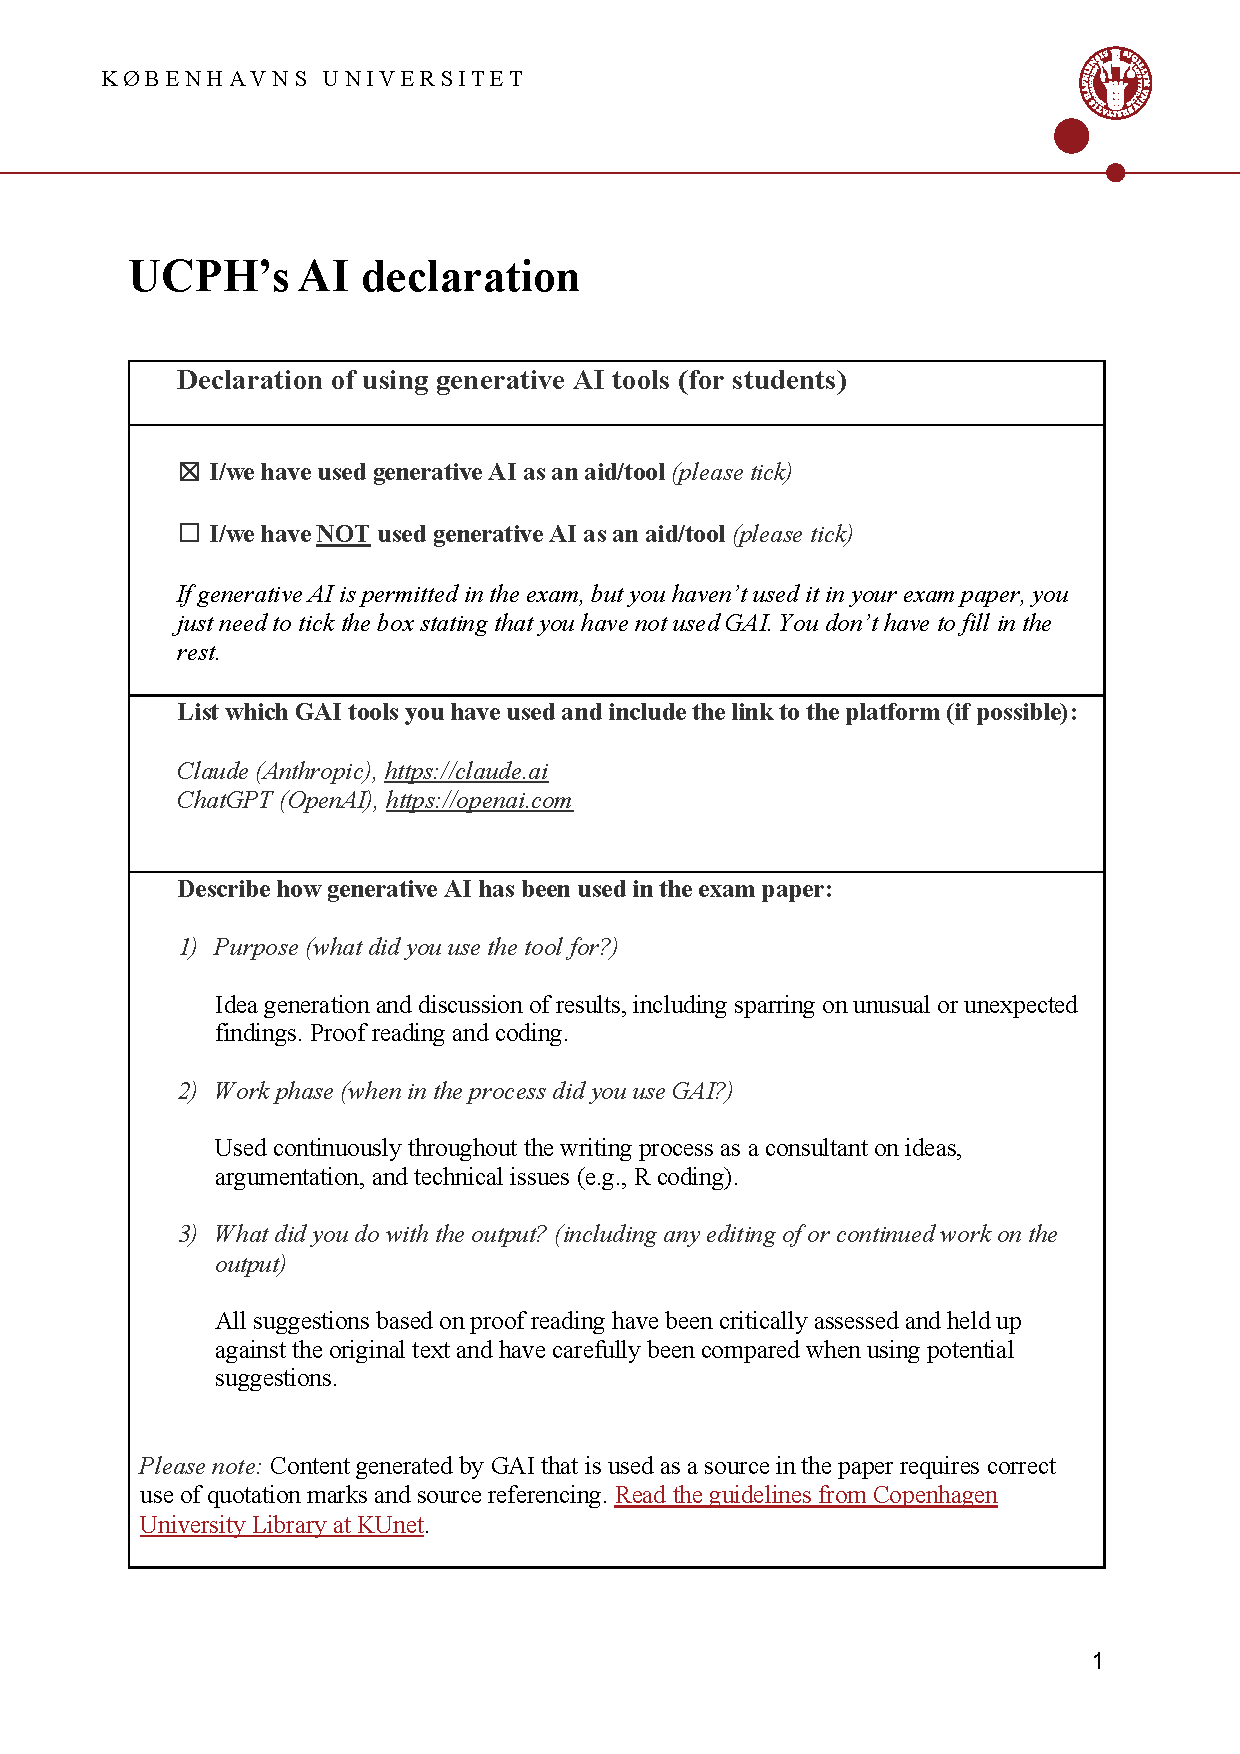
\includepdf[pages=-]{AI_declaration.pdf}


\newpage

\section*{Acknowledgements}

We would like to express our sincere gratitude to our supervisors, Mette Asmild, Arne Henningsen and Jakob Vesterlund Olsen, for their guidance, constructive feedback, and for their confidence in the project throughout the process.

We are also grateful to Arne Henningsen for granting access to necessary information from IFRO/DST production branch statistics, and to Jakob Vesterlund Olsen for providing the nitrogen leaching maps and for his assistance in obtaining and understanding the data. 
Finally, we thank SEGES for providing access to the farm accountancy data. 
In particular, we thank Jacob Sørensen for his technical assistance with Databricks, and for answering questions regarding the data set throughout the project.


\begin{table}[h]
\def\arraystretch{1.5}
\begin{tabularx}{\textwidth}{l X}
Faculty: & {The Faculty of Natural and Life Sciences}  \\
Department & {Department of Food and Resource Economics (IFRO)} \\
Authors: & {Helle Dahlgren Berlin (rns300) and William Louis Reingaard Vissing (vhs376)} \\
Title: & {Mapping Agricultural Profits and Environmental Costs at the Field-Level} \\
Advisors: & {Mette Asmild, Arne Henningsen, and Jakob Vesterlund Olsen} \\
Date: & {June 1, 2026}
\end{tabularx}
\end{table}


\newpage


\section*{Abstract}
This thesis develops and evaluates a pilot method for estimating field-level agricultural profitability incorporating both private economic returns and environmental costs of agricultural production. 
The model is based on farm accounting data from 894 Danish conventional farms in the year 2024 (SEGES) and builds on Danish production branch statistics developed by IFRO and Statistics Denmark. 
Farm-level accountancy data is disaggregated to field level by combining field data with spatial information on nitrogen leaching, retention, and damage costs, producing a spatially explicit data set linking economic returns and environmental impacts at field level.
A key innovation is that field-level profitability is estimated from observed farm accountancy data as gross margin II (DBII), rather than from standardised budget calculations. 
This provides a data-driven measure of spatial variation in agricultural profitability across geographical locations, crops, and soil types.

From society's perspective, the model extends DBII by incorporating estimated environmental damages from nitrogen leaching to coastal waters using both uniform and spatially differentiated damage cost estimates. 
A central methodological feature is the use of a standardised reference scenario, where all fields are evaluated under identical management conditions (continuous winter wheat under regulatory fertilisation norms). This isolates underlying biophysical vulnerability, including soil type, nitrogen retention capacity, and proximity to vulnerable coastal waters.

The results show substantial spatial variation in both economic returns and environmental costs across fields and catchments in 2024. Winter wheat exhibits a pronounced west-–east profitability gradient, while spring barley displays weaker spatial patterns and generally negative DBII across catchments. Incorporating environmental damages alters the spatial distribution of field-level profitability, highlighting considerable heterogeneity in the trade-offs between agricultural production and environmental impacts.

Overall, the thesis demonstrates the feasibility of constructing a spatially explicit, data-driven method for supporting agri-environmental policy design and land-use planning. The results suggest that combining field-level economic and environmental data may improve spatial targeting of land retirement and future agri-environmental regulation.



\newpage


\tableofcontents


\newpage



\section{Introduction}
\label{sec:introduction}

Denmark is one of the most intensively cultivated countries in Europe, with agriculture accounting for approximately 60 percent of total land area. 
Increasing demands on agricultural land to deliver not only food production but also broader environmental objectives such as climate change mitigation, nutrient reduction, biodiversity restoration, and groundwater protection have intensified competition over land use. 
These pressures are reflected in the Green Tripartite Agreement \citep{regeringen2024groentdanmark}, which aims to retire approximately 390,000 hectares of agricultural land, primarily through afforestation and wetland restoration \citep{regeringen2024groentdanmark}.

The dynamics reflect a broader European shift. Under the Common Agricultural Policy (CAP), biodiversity, clean water, and climate regulation are increasingly framed as public goods that markets systematically underprovide, thereby justifying a stronger focus on agri-environmental schemes  (AES) and a policy design that increasingly promotes performance- and result-oriented approaches within the CAP framework \citep{eu_ndm, eurochoices2025}.

This raises a central policy challenge: how to ensure that the most productive agricultural land remains in production, while environmental policies are targeted towards areas where social benefits are highest and economic costs are lowest. 
Addressing this challenge requires more spatially disaggregated information on both the productive value of agricultural land and the environmental impacts of cultivation.

A growing number of geospatial models and high-resolution gridded data sets are currently being developed to support such policy objectives. These include, among others, nitrogen retention maps \citep{Borgesen2020}, biodiversity maps \citep{petersen2024mere}, and groundwater voulnerability assessments currently under development \citep{miljostyrelsen_sgo}. However, few operational economic models exist that estimate profitability of agricultural production at the field level. 
This gap obscures the economic and environmental trade-offs involved in, for example, land retirement under the Green Tripartite Agreement.

The purpose of this thesis is to investigate the feasibility of developing an econometric model capable of estimating field-level profitability using 
farm-level accountancy data for 894 conventional farms 
in the year 2024 \citep{seges2025}. This thesis is conceived as a pilot study aimed at assessing whether existing data sources and econometric methods can support the development of a field level framework for land-use planning and environmental regulation.
More specifically, the thesis builds upon the methodology currently used by IFRO in the production branch statistics \citep{dst2025a,henningsen2026}, where accounting data from Danish farms is used to allocate input use from farm level to production branch level. 
In this thesis, the methodology is adapted with the purpose of allocating economic results from farm level to field level. 

The thesis examines profitability from both the farmer's and society's perspective. 
From the farmer's perspective, profitability is defined as field-level revenues minus production costs referred to throughout the thesis as DBII \footnote{DBII corresponds to “dækningsbidrag II” (gross margin II) in Danish agricultural accounting, defined as revenues minus variable and fixed production costs.}. From society's perspective, the profitability measure is extended to include the valuation of environmental externalities associated with agricultural production.
In principle, a fully developed model should incorporate the broad range of externalities linked to agricultural land use, including impacts on climate, biodiversity, groundwater quality, air pollution, ecosystem services, and human health. 

Given the scope of this pilot study, the analysis focuses specifically on damages arising from nitrogen leaching to coastal waters --- an externality of particular relevance in Denmark given its extensive coastline.

The broader ambition of this pilot study is to contribute to the development of a framework capable of supporting more cost-effective and spatially differentiated land-use regulation. If fully developed, such a framework could identify areas where agricultural production generates high economic value at relatively low environmental cost, as well as areas where the environmental benefits of land retirement are comparatively large relative to the forgone agricultural value. 
We argue that such a framework could play an important role both in the implementation of land retirement initiatives under the Green Tripartite Agreement and in the future design of more environmentally targeted agri-environmental schemes under the CAP. 

The thesis is structured as follows. Section~(\ref{sec:background}) reviews related literature and background information. 
Section~(\ref{sec:welfare-economic-framework}) describes the welfare economic framework adapted in the thesis.
Section~(\ref{sec:data}) describes the data which the empirical analysis is based on.
Section~(\ref{sec:methodology}) presents the empirical method.
Section~(\ref{sec:results}) presents and evaluate the results.
Section~(\ref{sec:Limitations}) discusses the limitations of the analysis.
Section~(\ref{sec:discussion}) discusses the results and their implications in light of the identified limitations.
Section~(\ref{sec:conclusion}) concludes on the main findings. 


\newpage


\section{Background}
\label{sec:background}
This section situates the thesis within the existing literature and provides context for the empirical analysis. It begins by reviewing Danish studies on the economic assessment of agricultural land use, before turning to the role of field-level profitability in spatial optimisation and nitrogen regulation. 
Furthermore, some of the conditions for the crop production economy in 2024 are viewed to contextualise the field-level estimates presented in the thesis.

\subsection{Economic Assessment of Agricultural Land Use}
A few Danish studies have sought to map the economic contribution of agricultural production at a spatially disaggregated level. \cite{Jensen2010}~takes an early step in this direction by combining the General Agricultural Register and the Central Livestock Register  - which together provide structural information on land use, crop composition, and livestock holdings - with farm accounting data on costs and revenues. Since economic data are available only for a limited sample of farms, \cite{Jensen2010}~applies an approximation method assuming that farms with similar structural characteristics have similar economic outcomes. This enables geographical mapping of farm-level production and net income, highlighting how economic activity is distributed across regions. 

Building on this, \cite{Pedersen2022}~develops an approach to map cultivation values for Danish agricultural land at a 100$\times$100 m spatial resolution, calculating DB II based on crop-specific budget calculations adjusted for soil type, field size, and livestock density. A 12-year cultivation history is used to account for crop rotations and reflect farmers' production choices. While this budget-based approach represents an important methodological advance, it relies on standardised assumptions regarding crop prices, revenues, and costs rather than observed farm-level data. \cite{Pedersen2022}~acknowledges this as a key limitation, noting that estimates based on observed farm accountancy data differentiated by crops and soil types would constitute a more empirically grounded alternative. 

While~\citet{Jensen2010} provides economic detail without field-level resolution and~\citet{Pedersen2022} achieves spatial resolution without observed economic data, neither approach combines field-level spatial resolution with empirically grounded profitability estimates. This thesis addresses this gap by integrating both elements within a single framework.



\subsection{Spatial Optimisation and Nitrogen Regulation}

Estimating field-level profitability is highly relevant in the context of nitrogen regulation, where cost-effective targeting requires information on both the environmental burden and the economic value of individual fields. A central challenge in designing such regulation is the need to account for spatial 
heterogeneity in both the environmental impacts of nitrogen losses and the economic value of agricultural production. 
Two recent contributions are particularly relevant to this thesis.

\cite{Termansen2023}~develop a spatial optimisation model, building on the cost-minimisation framework of TargetEconN~\citep{Hansen2019}, to identify where land-use changes --- such as afforestation, wetland restoration, and buffer zones --- can achieve environmental goals related to water quality, climate, biodiversity, and recreation at the lowest cost. The model incorporates opportunity costs of agricultural production based on crop--specific budget calculations, spatially differentiated retention and leaching data, and biodiversity indices, enabling scenario analyses that account for synergies and trade-offs across multiple environmental objectives~\citep{Termansen2023}.

\cite{Olsen2026}~analyse the cost-efficiency and distributional effects of a framework for discharge-based nitrogen quota regulation developed as part of the NUAR project (Ny Udledningsbaseret ArealRegulering), initiated under the 2021 Danish Agricultural Agreement. The project represents a shift from reduction-based to discharge-based regulation, using field-level estimates of nitrogen leaching to improve spatial targeting in relation to Water Framework Directive targets. The economic analysis in NUAR is based on Kalkule Mark~\citep{Hvid2023}, a budgeting tool based on standardised crop prices and fertilisation norms rather than observed farm accounting data.
 
Together, these studies highlight a central gap in the literature: while spatial environmental models and regulatory design analyses are increasingly sophisticated, the economic valuation of agricultural production at the field level -- based on observed farm accountancy data rather than budget calculations -- remains underexplored in a Danish context. 
 
This thesis addresses this gap by estimating field-level profitability directly from observed farm accounts, providing an empirically grounded measure of agricultural value. It does so, by building on the production branch statistics methodology~\citep{henningsen2026}, which IFRO carries out annually on behalf of Statistics Denmark and the Ministry of Food, Agriculture and Fisheries, allocating costs from farm level to production branches. We extend this framework one step further by allocating both inputs and outputs to individual fields using observed farm accounting data. This extension enables us to capture actual variation in field-level profitability across farms, soil types, and crops, rather than approximating it through standardised budget calculations. By integrating nitrogen damage cost estimates, the framework further extends this measure to a societal perspective, capturing the trade-off between agricultural production and environmental externalities at the field level (see Section~\ref{sec:estimating-damage-costs}). \\[0.25cm]


\subsection{Crop Production Economy in 2024}

The economic conditions for Danish crop producers in 2024 provide important context for interpreting the field-level profitability estimates in this thesis. Drawing on \cite{bramsen2024}, this subsection summarises the key production and price conditions for the main crops considered.
  

\subsubsection{Weather Conditions}
\label{sec:Weather Conditions}
The 2024 growing season was characterised by exceptionally high precipitation. Total rainfall from October 2023 to October 2024 reached 1,106 mm, approximately 50 percent above the climatological normal of 759 mm~\citep{dmi2026}. 
Waterlogged soils delayed field operations in spring, postponed fertiliser application on winter crops, and pushed establishment of spring crops well beyond optimal sowing dates~\citep{bramsen2024}.

\begin{figure}[H]
\centering
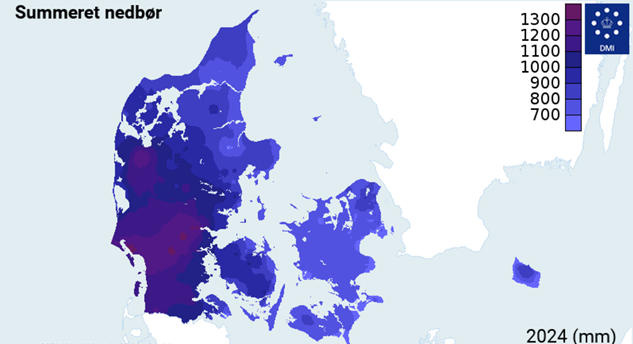
\includegraphics[width=0.95\textwidth]{figures/Nedbør.png}
\caption{Total annual precipitation (mm) in Denmark in 2024. Source:~\citet{DMI2025}.}
\label{fig:dmi_nedbor}
\end{figure}

As shown in Figure~\ref{fig:dmi_nedbor}, rainfall was spatially uneven, ranging from 738 mm in 
western and southern Zealand to 1,146 mm in southern Jutland~\citep{DMI2025}. 
Southern and central Jutland were particularly affected by excess water, while eastern Denmark experienced comparatively drier conditions~\citep{bramsen2024}.
This spatial variation translated into substantial variation in farm-level economic outcomes, with some regions reporting near-normal harvests while others suffered severe losses. 

%For large arable farms with at least two full-time employees, the average operating 
%result before remuneration of the farm family was projected to fall from 
%approximately DKK 890{,}000 in 2023 to DKK 220{,}000 in 2024~\citep{bramsen2024}. 


\subsubsection{Selected Crops}
\label{sec:SelectedCrops}


Figure~\ref{fig:yield-development} shows that yields (hkg/ha) fell below normal levels\footnote{\cite{bramsen2024} calculate normal yield levels as Olympic averages of the last five years -- that is, the average over five years, with highest and lowest yielding years removed.} across all major cash crops in Denmark. The yield shortfalls, together with the broader market conditions, are summarised below for the crops most relevant to this thesis: spring barley and winter wheat.

\begin{figure}[H]
    \centering
    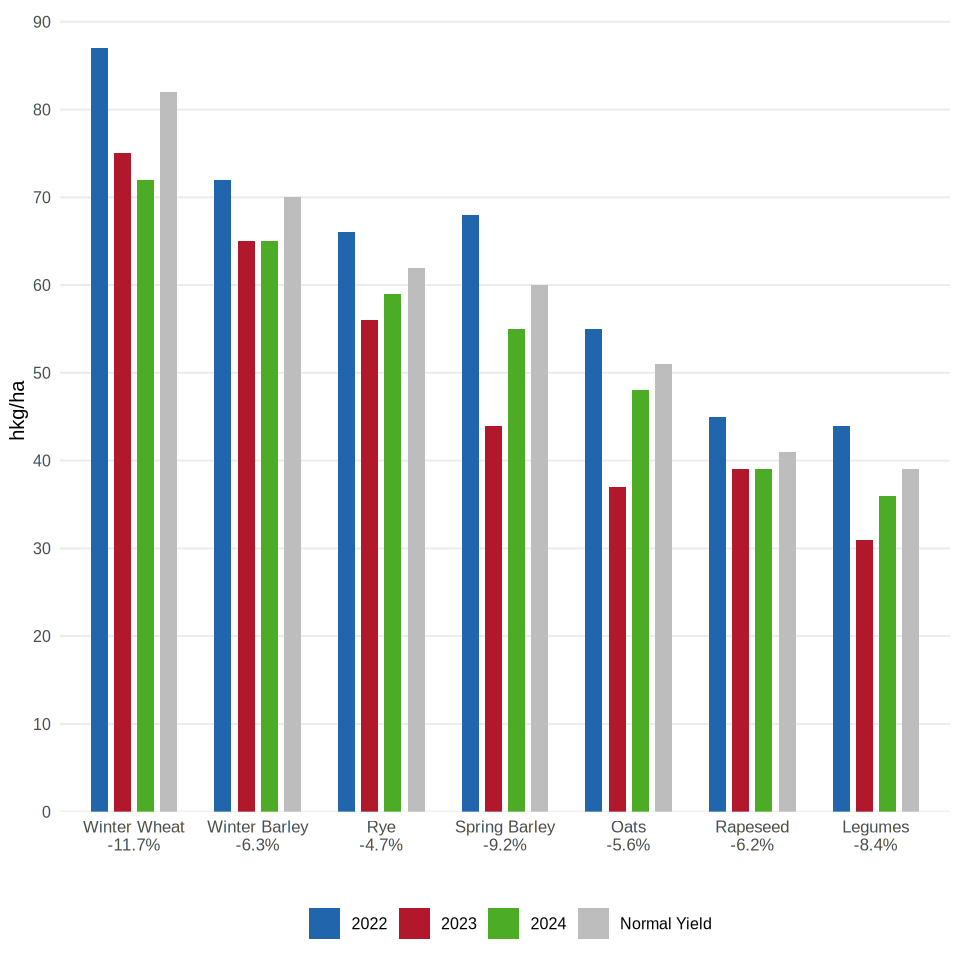
\includegraphics[width=0.7\textwidth, height=0.5\textheight, keepaspectratio]{figures/hist_yield_development.png}
    \caption{Yield per hectare (hkg/ha) for selected crops \citep{dst2026}}
    \label{fig:yield-development}
\end{figure}

\paragraph{Spring barley} is the largest crop by area in Denmark, covering approximately 512,000 hectares, but is generally among the least profitable crops in the rotation. In 2024, yields were 9.2 percent below normal. Combined with lower grain prices --— fully reflected in revenues for the first time since the 2021–-2022 price spike --- and higher interest costs, this resulted in particularly weak economic outcomes for spring barley producers \citep{bramsen2024}.

\paragraph{Winter wheat}
is the second largest crop by area with approximately 
465{,}000 hectares, and experienced the largest decline in yields among the major 
crops in 2024, at 11.7 percent below normal. 
As the dominant high-yielding cash crop in Danish agriculture, this reduction in yield carried substantial weight in the aggregate economic outcome for arable 
farms. 
Lower market prices passed fully through to revenues in 2024, amplifying 
the impact of the poor harvest  \citep{bramsen2024}.

%\paragraph{Rapeseed, Potatoes, and Other Crops.}
%Beyond the major cereals, rapeseed yields were approximately 6.2 percent
%below normal in 2024 \citep{bramsen2024}, though the crop continued to
%provide relatively attractive returns compared to cereals.
%Sugar beet experienced both lower yields and lower prices, while grass
%seed production was affected by reduced area and lower prices.
%Fodder crops, grown primarily for internal use in livestock production,
%are valued at internal transfer prices rather than market prices, which
%limits the direct interpretability of their profitability and motivates
%the cautious treatment of these crops in our analysis.

\subsubsection{Potential Implications for the Empirical Analysis}
Two features of 2024 are particularly relevant for interpreting the
field-level profitability estimated in this thesis.
First, the below-normal yields across all major cereals --- including
winter wheat and spring barley --- imply that our field-level estimates of
profitability for these crops should be regarded as conservative relative
to a long-run average.
Second, the geographic variation in weather conditions implies that part
of observed spatial variation in field-level profitability across coastal
catchment areas may reflect the specific weather conditions of 2024,
in addition to underlying differences in soil productivity.


\section{Welfare Economic Framework}
\label{sec:welfare-economic-framework}

From a welfare economic perspective, agricultural land use should be evaluated in terms of its contribution to social welfare, defined as the difference between social benefits and social costs. This requires accounting for both the private value of agricultural production and the value of any associated externalities.

In this thesis, the relevant externality is nitrogen leaching from agricultural fields to coastal waters. Although nitrogen use is regulated through policy instruments such as fertiliser norms and mandatory catch crops, these mechanisms do not fully internalise the associated environmental damages. As a result, a wedge remains between private and societal profitability.




%Agricultural production generates both private returns and broader social costs and benefits that are not fully captured by market prices.
%This thesis adopts a welfare economic framework that underpins the 
%empirical analysis, drawing on the theory of production externalities to 
%motivate the inclusion of environmental damages.

%\subsection{Profitability from Farmer's Perspective}
%From the farmer's perspective, the decision to cultivate a given field is governed by private profitability --- the difference between revenues from agricultural output and the costs of production inputs.
%A rational farmer will continue to cultivate a field as long as the private return is non-negative, taking input and output prices as given.
%However, some agricultural production is associated with environmental externalities --- costs that are generated by third parties and not fully reflected in the farmer's production plans.

%A common textbook example is a firm that produces a desirable output alongside an undesirable by-product that imposes costs on others.
%The profit-maximising firm will produce the by-product up to the point where its own marginal cost of generating an additional unit equals zero, since it faces no price for the environmental damage it causes.
%From a social perspective, however, the optimal level requires equating the marginal private benefit of the polluting activity with the marginal social cost, which includes the damages imposed on affected parties.
%The divergence between private and social costs leads the unregulated market to overproduce the externality relative to the social optimum.

%In the context of this thesis, the relevant externality is nitrogen leaching from agricultural fields to coastal waters.
%Nitrogen applied to fields as fertiliser is only partially taken up by crops, and the residual leaches into waterways, eventually reaching coastal ecosystems where it contributes to eutrophication and associated ecological damages.
%These damages represent a social cost of agricultural production that the farmer has no private incentive to internalise, absent regulation or a tax set equal to the marginal external damage.

%\subsection{Profitability from Society's Perspective}
%Following the welfare economic framework, the socially optimal allocation of land between agricultural production and alternative uses --- such as wetland restoration or afforestation --- requires comparing the social benefits and social costs of cultivation at each location.
%The social benefit of cultivating a given field is the private value of agricultural production, while the social cost includes both the private production costs and the external environmental damages associated with nitrogen leaching.

%This framework provides the economic rationale for spatially targeted agri-environmental policy: rather than applying uniform regulations or payments across all agricultural land, policy instruments should ideally be directed towards fields where the ratio of environmental damage to private value is highest --- that is, where the net social gain from land-use change is largest.

\subsection{Definition of DBII}
\label{sec:dbii-definition}

To operationalise these concepts, two profitability measures are used in the empirical analysis. Private profitability is measured by field-level profitability from the farmer's perspective ($\mathrm{DBII^{farmer}}$), defined as revenues minus production costs. 
Social profitability is measured by field-level profitability from society's ($\mathrm{DBII^{society}}$) perspective extended by subtracting environmental damages from nitrogen leaching:
\begin{equation}
\begin{aligned}
    \label{eq:def-dbii}
    \text{DBII}^{\text{farmer}} &= \text{Revenues} - \text{Costs} \\
    \text{DBII}^{\text{society}} &= \text{Revenues} - \text{Costs} - \text{Social Damage Costs}
\end{aligned}
\end{equation}


The definition of DBII follows the production branch statistics at 
Statistics Denmark \citep{dst2025a}, extended in line with SEGES' conventions 
to include semi-variable and fixed costs alongside variable costs 
\citep{seges2022}.
Environmental subsidies are excluded, as they 
reflect policy transfers rather than production-related value, and would otherwise conflate private economic returns with public compensation.

The empirical construction of the farmer's revenues, costs, and social costs is described in Section~\ref{sec:methodology} and detailed in 
Appendices~\ref{sec:gross-margin-ii}--\ref{sec:revenues}, while the modelling of nitrogen leaching and social damage costs are described in 
Section~\ref{sec:estimating-damage-costs}.

\section{Estimating Nitrogen Damage Costs}
\label{sec:est-nitrogen-damage-costs}

Nitrogen pollution from agriculture is associated with substantial environmental damages in aquatic ecosystems, including eutrophication and deterioration of coastal water quality. These damages may further affect ecosystem services and non-market values such as recreational opportunities and aesthetic quality \citep{Keeler2016,brink2011}.

%Nitrogen pollution from agriculture is associated with substantial environmental damage, including eutrophication, biodiversity loss, algal blooms, oxygen depletion, and ecosystem degradation in marine environments \citep{Keeler2016}. Nitrogen pollution also impair landscape aesthetics and reduce ecosystem services such as recreational opportunities \citep{brink2011}. 



Both nitrogen losses and resulting environmental damages vary substantially across locations due to factors such as soil characteristics, climate, hydrology, farming practices and proximity to vulnerable coastal ecosystems. Consequently, the social cost associated with nitrogen pollution is inherently spatial and may differ substantially between otherwise similar fields.



The purpose of this section is to establish the process by which a quantity of nitrogen leached from individual fields, ultimately reaches coastal waters and to translate these losses into monetary damage costs. % These environmental costs are subsequently incorporated into field-level profitability estimates in order to derive a proxy for the societal profitability of agricultural production at the field level.  



%The analysis is based on a standardised reference scenario assuming continuous winter wheat production under standardised regulatory fertilisation norms. This reference scenario is combined with spatially explicit models of nitrogen leaching and retention. Consequently, estimated outcomes should be interpreted as potential nitrogen losses under a common management regime rather than realised field-level emissions. While this assumption is necessary to ensure comparability across fields, it abstracts from heterogeneity in observed crop rotations, mitigation measures, and farm-level management practices.



The following sections introduce the concepts of nitrogen leaching and retention and describe the underlying spatial modelling framework. Subsequently, the economic valuation literature used to derive nitrogen damage cost estimates is presented.

\subsection{Nitrogen Leaching from the Field}
Nitrogen leaching is defined as the fraction of nitrogen that moves below the root zone where it is no longer available for plant uptake and is considered a loss from the field. It is primarily driven by the cropping system, with crop choice, fertiliser application rate and timing, soil type, precipitation, cover crops, and drainage all influencing the magnitude of losses. Leaching is considered to be the dominant pathway of nitrogen (N) losses from agriculture, and is typically estimated using empirical models such as NLES5 and Daisy \citep{Borgesen2020}.

\subsubsection{Leaching Maps for Winter Wheat and Spring Barley}
\label{Leaching Map for Continuous Winter Wheat and Spring Barley}

We employ a nitrogen leaching map for winter wheat following winter wheat as a reference \citep{Olsen2026}  and spring barley with catch crops following spring barley \citep[unpublished]{OlsenNd} as a robustness analysis. Both maps are kindly made available for this thesis by Jakob Vesterlund Olsen. The maps are based on the NLES5 model as described in \cite{Borgesen2020} and quantifies estimated leaching in kg N per hectare.

NLES5 predicts annual nitrate leaching (April--March) as a function of crop choice, crop rotation, catch crops, fertiliser level, soil type (clay content in topsoil), and water percolation. Although leaching occurs primarily during autumn and winter, the model captures hydrological conditions through percolation measures both within and outside the growing season, and explicitly accounts for the effects of both main crops and winter vegetation in the current and preceding year \citep{Borgesen2020}. The model further distinguishes between spring- and autumn-applied nitrogen, reflecting their different leaching risks. Nitrogen inputs include mineral and organic fertilisers, manure, grazing, and biological fixation, and are considered for both the current year and as an average over previous years, allowing the model to capture both immediate and lagged effects of nitrogen application \citep{Borgesen2020}.

NLES5 is a statistical model estimated on experimental and monitoring data, primarily from Denmark, and is designed to capture spatial variation in leaching driven by differences in soil properties and climatic conditions, making it well suited for generating spatially explicit leaching maps \citep{Borgesen2020}. 

By applying the winter wheat leaching map we assume a uniform cropping system applied on a national scale. Additionally, the leaching maps are based on regulatory fertiliser norms, thereby abstracting from actual fertilisation rates. As spatially detailed leaching maps for alternative crop rotations are not yet available for our purpose, the winter wheat map serves as a reference for all fields in the data set. We apply the spring barley with a catch crop following spring barley as a sensitivity analysis to evaluate how robust the reference scenario is to the choice of refererence crop. However, the spatial resolution of the two maps differs. The winter wheat leaching map quantifies estimated leaching in kg N per hectare at a spatial resolution of 1 ha (100 $\times$ 100 m) (Børgesen et. al., 2020) whereas the spring barley map is more aggregated and based on a spatial resolution following the ID44, which represents a coarser regional zoning. As a consequence, the two maps are not directly comparable in spatial detail.


\subsection{Nitrogen Retention}
When nitrogen is leached from the root zone, it is transported via groundwater or drainage systems to surface waters (streams, lakes, and wetlands) and ultimately to the sea. During this transport, part of the nitrogen---primarily as nitrate---is converted to gaseous nitrogen through denitrification (nitrogen retention) and released to the atmosphere. This process occurs under low-oxygen to anoxic conditions in both groundwater and surface water systems. Due to spatial variation in geology, hydrology, redox conditions, and drainage placement relative to the redox zone, nitrogen retention varies considerably across locations 
\citep{Hojberg2025}.

\subsubsection{Retention Map}
The transport of nitrogen from the root zone to coastal waters is modelled using the updated national nitrogen model (NKMv2025), developed by GEUS and Aarhus University and calibrated against the NOVANA monitoring programme \citep{Hojberg2025}. The model describes the transport and transformation---including denitrification---of nitrogen from the root zone to the coast. Retention is calculated on a 100 $\times$ 100 m grid and reported as the percentage of nitrogen retained relative to the amount leached from the field. Compared to previous versions, the map is significantly more spatially detailed, reflecting a policy ambition to enable farm-level regulation of nitrogen losses 
\citep{Hojberg2025}.

Nitrogen leaching from agricultural land is estimated using the NLES5 model. Water balance and monthly runoff are simulated using the Daisy model based on DMI data \citep{Hojberg2025}. Land use is represented through GIS-based field maps, crop reporting, and fertiliser accounts, allowing farming practices and mitigation measures (e.g.\ catch crops and wetlands) to be 
incorporated at field level. The model reflects agricultural practices up to 2021, including reduced fertiliser use and increased adoption of catch crops \citep{Hojberg2025}.

Nitrogen transport and transformation in groundwater and surface water are modelled by coupling the NKM to the national hydrological model (DK model; Stisen et al., 2019) and the hydrostratigraphic model (FOHM; Miljøstyrelsen), which describe flow pathways and geological conditions. 
Retention is thus modelled across three components: (1) retention/leaching from the root zone, (2) retention in groundwater, and (3) retention 
in surface water \citep{Hojberg2025}.

% The updated retention map applied here provides a more spatially precise basis for targeting than earlier catchment-based approaches, such as ID15 averages \citep{Hojberg2025}.

%Retention is calculated on a 100 $\times$ 100 m grid and reports rentention as a percentage of the nitrogen leached form the field. The updated retention map applied here provides a more spatially precise basis for targeting than earlier catchment-based approaches such as ID15 averages \citep{Hojberg2025}. 

%Due to data limitations results are aggregated using a region-growing method, grouping adjacent areas with similar retention values into regions of at least 50 hectares---providing a more spatially precise basis for targeting than earlier catchment-based approaches such as ID15 averages \citep{Hojberg2025}. 

Uncertainty in the retention map is assessed using Monte Carlo simulations and comparisons between observed and modelled nitrogen transport. For monitored catchments, uncertainty is reduced through calibration to observations, whereas unmonitored areas are corrected at a 
more aggregated level. Overall uncertainty is estimated at below 10 percentage points for 90 percent of observations, though this is assumed to be an underestimation in areas distant from monitoring stations or with complex hydrogeological conditions \citep{Hojberg2025}.

\subsection{Estimating Nitrogen Damage Costs}
\label{sec:estimating-damage-costs}

This section describes how nitrogen damage costs are estimated at the field level. Two valuation approaches are applied. The first uses catchment-specific damage cost 
estimates derived from \citet{andersen2019}, available for six of the eleven catchments included in the analysis. The second applies a uniform EU-average damage 
cost estimate derived from the European Nitrogen Assessment \citep{brink2011}, which is applied across all eleven catchments. The two approaches differ in scope 
and are not directly comparable, but together allow for an assessment of how sensitive the spatial distribution of estimated damage costs is to the choice of 
valuation method. The catchments covered by each approach are illustrated in Figure~\ref{fig:catchments}.

\begin{figure}[H]
\label{fig:catchments}
\centering
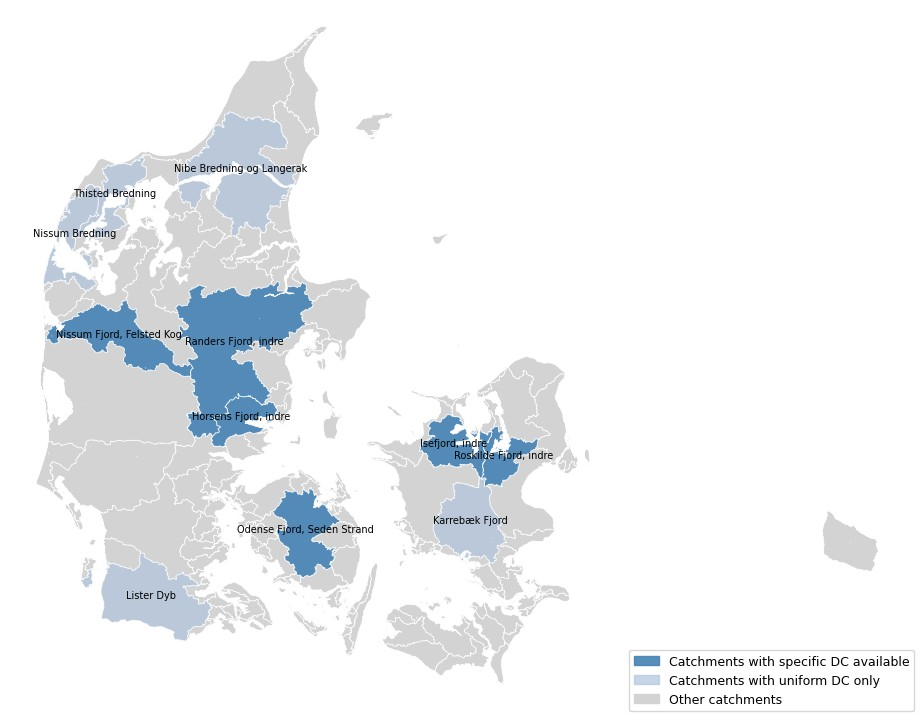
\includegraphics[width=0.95\textwidth]{figures/catchment1.jpg}
\caption{Catchments included in the empirical analysis. Dark blue catchments 
have location-specific damage cost estimates available; light blue catchments 
are covered by the uniform approach only.}

\end{figure}

\subsubsection{The Specific Valuation Approach}

\label{sec:specific-valuation-approach}

For six out of the eleven catchments included in this thesis, location-specific estimates from \citet{andersen2019} are used as proxies for damage cost per kilogram of nitrogen reaching coastal waters. These estimates reflect welfare effects through changes in recreational and amenity values as well as property prices, and should therefore be interpreted as partial estimates of total damages.

\cite{andersen2019} does not directly estimate marginal damage costs. Instead, they derive economic benefits of reducing nitrogen pollution under a specific policy scenario. More specifically, the authors compare a baseline scenario (reflecting observed nitrogen loads around 2010) with a policy scenario involving a 35\% reduction in agricultural nitrogen leaching needed to comply with the Water Framework Directive (WFD) on “good ecological status” \citep{andersen2019}. This reduction leads to improvements in water quality, measured as increased water clarity (Secchi depth), which in turn generates economic benefits \citep{andersen2019}.




To estimate these benefits, \cite{andersen2019} apply an impact pathway approach linking (1) nitrogen loads from catchments, (2) nitrogen concentrations in estuaries, (3) water clarity (Secchi depth), and (4) economic valuation of improved water quality through property prices and recreational use via benefit transfer.

%\begin{enumerate}
%    \item nitrogen loads from catchments,
%    \item nitrogen concentrations in estuaries,
%    \item water clarity (Secchi depth), and
%    \item economic valuation of improved water quality through property prices and recreational use via benefit transfer.
%\end{enumerate}


The key element for the present analysis is how the aggregate benefits are converted into a per-unit value. Assuming proportionality, the total estimated welfare gain from the policy scenario is divided by the corresponding reduction in nitrogen loads. This yields an average benefit per kilogram of nitrogen reduced, which we interpret as a proxy for the damage cost per kilogram of nitrogen:
\begin{align*}
    \text{Social damage cost} \approx \frac{\text{Total welfare gain}}{\text{Total nitrogen reduction}}
\end{align*}

The use of these estimates as per unit damage costs is not without limitations. They are derived from a specific policy scenario -- a 35\% reduction relative to the 2010 baseline -- and do not reflect current regulatory conditions. If nitrogen loads to coastal waters have declined since 2010 as a result of continued regulation, the damage cost per kg N at current pollution levels may differ from the estimates derived under the 2010 baseline scenario.




Nevertheless, eutrophication in fjords and coastal waters remains a significant issue. Importantly, the estimates provide valuable information on relative differences in damage costs across locations. Such spatial variation is critical, as substantial heterogeneity exists across catchment areas. Differences in nutrient loads, hydrological conditions, and baseline ecological status imply that identical reductions in nitrogen can lead to different improvements in water clarity and associated welfare gains \citep{andersen2019}.



These estimates should be interpreted as lower-bound damage costs. \cite{andersen2019} focus on recreational benefits and property values because these can be directly linked to observable changes in water clarity and supported by empirical willingness-to-pay estimates \citep{andersen2019}. Other impacts such as biodiversity improvements are not included, partly due to limited empirical evidence and partly because such benefits tend to materialize over longer time horizons and are typically low when discounted to present values \citep{andersen2019}.



Other sources of uncertainty should be acknowledged. These include uncertainties in the ecological relationships between nitrogen concentrations and water clarity, the transferability of valuation estimates across contexts (benefit transfer), and the assumption of constant damage over the range of nitrogen reductions considered. Despite these limitations, the estimates are considered the most suitable available for capturing location-specific damage costs. Applied damage cost estimates are presented in Table \ref{tab:damage-costs}, reported in 2024 prices. 

\begin{table}[htbp]
\centering
\small
\caption{Damage Cost Estimates}
\label{tab:damage-costs}
\begin{threeparttable}
\begin{tabular}{lrr}
\toprule
ID15 Coastal Catchment & Code & DKK/kg N \\
\midrule
Roskilde Fjord, indre   & 2   & 74.34  \\
Odense Fjord, Seden Str.& 93  & 44.04  \\
Horsens Fjord, indre    & 128 & 87.80  \\
Nissum Fjord, Felsted Kog& 131 & 11.99  \\
Randers Fjord, indre    & 136 & 21.93  \\
Isefjord, indre         & 165 & 69.34  \\
\midrule
Uniform$^{a}$           &  $-$  & 130.76 \\
\bottomrule
\end{tabular}
\begin{tablenotes}
\footnotesize
\item \textit{Notes:} Damage cost estimates are derived from 
\cite{andersen2019}. \\
$^{a}$ Mean value of the bounds [52.30--209.21] DKK per kg N., based on the European Nitrogen Assessment 
\citep{brink2011}. Table reflects 2024 prices (Appendix \ref{fig:DC_calc}).
\end{tablenotes}
\end{threeparttable}
\end{table}

\subsubsection{The Uniform Valuation Approach}

We apply the social damage cost of nitrogen pollution to surface waters from the European Nitrogen Assessment (ENA) \citep{brink2011}. Although these estimates are from 2011, they represent the most comprehensive Europe-wide assessment of nitrogen damage costs currently available. In the absence of more recent alternatives, they provide the most appropriate basis for a uniform per-unit valuation of nitrogen damage costs in this thesis.

The unit damage costs for the loss of ecosystem services due to nitrogen (N) in \cite{brink2011} are based on a synthesis of multiple studies rather than a single integrated model, and it is therefore important to understand their derivation and limitations. The authors compile and convert results from a range of valuation studies into per-kilogram costs of reactive nitrogen (Nr). These include freshwater eutrophication costs (e.g., Pretty et al., 2003), where total damages to recreational use, property values, and drinking water production translate to a low unit cost of around 0.3 EUR per kg N (in 2005 prices). Willingness-to-pay studies for improved water quality in the Baltic Sea (Söderqvist and Hasselström, 2008) produce higher average unit damage costs of approximately 12 EUR per kg N, with substantial regional variation. Restoration costs for biodiversity losses, as estimated in the NEEDS project, provide lower-bound estimates of roughly 2--2.5 EUR per kg N. Overall, \cite{brink2011} combine cost-based and willingness-to-pay approaches to produce broad, average estimates of nitrogen-related damage costs, which should be interpreted as indicative and subject to extensive uncertainty.



Notably, the WTP study for a clean Baltic Sea showed higher willingness-to-pay values for Nordic households compared to households in the Baltic states, highlighting a key limitation: applying uniform damage cost estimates across the EU oversimplifies spatial variation. Unlike location-specific estimates such as those in \cite{andersen2019}, uniform values do not account for local ecological and socio-economic conditions. Nevertheless, by including these estimates, we assess how the application of specific versus uniform damage costs influences the total damage cost for a given catchment. 



Within the limits of a master's thesis, we consider these estimates to be among the best available. \cite{brink2011} report upper and lower bound values for marginal damage costs of N pollution of surface waters. In this analysis we apply the mean value of these bounds in 2024 prices (Tabel~\ref{tab:damage-costs}).




\section{The Winter Wheat Reference Scenario}

\label{sec:The Winter Wheat Reference Scenario}

While we estimate profitability at the field level for multiple crops, detailed nitrogen leaching estimates are currently only available for stylised cropping systems. Consequently this study applies a winter wheat reference scenario to assess leaching potential across all fields on a consistent and comparable basis. Consequently, all fields are treated as if cultivated under continous winter wheat.

% combining it with average DBII for winter wheat differentiated by soil type and catchment. All fields are treated as if cultivated under continuous winter wheat. 
  



The choice of winter wheat is motivated by its status as the second most cultivated crop in Denmark in terms of area as well as its status as the dominant hight-yielding cash crop in Danish agriculture \citep{bramsen2024}. additionally Winter wheat is also used as reference crop within the NUAR framework \citep{Eriksen2024}. The reference scenario assumes fertilisation according to regulatory norms for winter wheat, differentiated by soil type. Consequently, all fields are treated as if managed under standardised regulatory conditions, independent of observed crop rotations and farm-level management practices. 

While this abstraction may overstate leaching in fields with mitigation measures such as catch crops, or reduced fertilisation, it provides a consistent baseline for spatial comparison across fields and avoids confounding from endogenous management choices. Combined with retention modelling, the approach enables identification of fields that (potentially) contribute disproportionately to nitrogen loads at the catchment level, rather than prediction of farm-specific outcomes.



Damage costs are subsequently applied to translate nitrogen losses into monetary terms. To assess the profitability of cultivating a given field under the standardised reference scenario, we estimate the average field-level profitability for winter wheat in 2024, calculated for each soil type within each catchment area (section \ref{sec:farmer-profitability}). This mean value is interpreted as an approximate measure of average field-level profitability from the farmer's perspective for winter wheat cultivation and is assigned to all fields according to their predominant soil type and catchment belonging. 
Estimated nitrogen damage costs are then subtracted to derive a proxy for net profitability from society's perspective under the reference scenario.

The analysis applies both uniform and location-specific nitrogen damage cost estimates, allowing for comparison and assessment of sensitivity to spatial variation. However, the framework does not explicitly capture potential non-linearities in damage functions and relies on damage cost estimates that are subject to considerable uncertainty. In addition, the use of a single-year average DBII for winter wheat introduces sensitivity to annual fluctuations in prices and yields; a multi-year average would likely provide a more robust representation of the reference scenario.

Despite these limitations, the approach combines estimates of nitrogen leaching from the root zone and its transport to coastal waters with economic valuation in a consistent way across all fields. This allows field-level profitability to be assessed from society's perspective in a comparable manner. The aim is not to predict farm-level behaviour, but to support spatial comparison and policy-relevant assessment of environmental impacts.





We replicate the main analysis using spring barley with a subsequent catch crop as an alternative reference scenario. Spring barley is the most cultivated crop in Denmark by area \citep{bramsen2024} and therefore provides a relevant robustness check on the choice of reference crop. The inclusion of a catch crop reflects common mitigation practice and allows for assessment of how sensitive the estimated spatial patterns in nitrogen leaching and associated economic outcomes are to alternative but agronomically plausible management assumptions. This comparison provides insight into the extent to which results are driven by the choice of reference crop versus underlying biophysical and spatial characteristics.

Strengths and limitations in the use of a winter wheat reference scenario is discussed in section~\ref{The Use of Average DBII Estimates}


\section{Data}
\label{sec:data}
The primary data source consist of farm-level accountancy data provided by SEGES and covers farms located within the eleven ID15 coastal catchments shown in figure~\ref{fig:catchments} \citep{seges2025}. 
The initial selection of catchments was determined by SEGES and included Lister Dyb, Randers Fjord (inner), Nibe Bredning og Langerak, Nissum Bredning, Thisted Bredning, Isefjord (inner), and Karrebæk Fjord. 
Access was subsequently expanded to four additional catchments --- Odense Fjord, Seden Strand, Horsens Fjord (inner), and Roskilde Fjord (inner) --- in order to improve geographical representation and align the sample with  catchments for which catchment-specific damage cost estimates were available.



Only farms with accountancy data approved for statistical purposes and with a registered CVR address within the relevant catchment area are included. To ensure representativeness, the approved accounts are weighted by SEGES in collaboration with Statistics Denmark based on four strata: full-time versus part-time farming, conventional versus organic production, farm type, and farm size measured by turnover. 

 
Table~\ref{tab:sample-restrictions} illustrates how the initial farm-level sample size of 1,077 farms is progressively restricted to the final analytical sample. 
Farm and fertiliser accounts are merged to include nitrogen variables in the estimation of input use.
Moreover, we exclude farms with zero crop production share in total production, and farms with a noteable horticultural production\footnote{See the distribution of the share of horticultural production in total production in Appendix~\ref{sec:data-prep-figures}.}, as their input structures differ substantially from those of conventional crop producers. 
Farms unsuitable for analyses have missing values or values equal to zero for inputs, revenues and field areas, as well as all farms with no fields in any of the eleven ID15 coastal catchments.
The final sample therefore consists of 894 conventional farms cultivating 23,336 fields.

\begin{table}[H]
\centering
\caption{Sample Restrictions and Farms Removed}
\label{tab:sample-restrictions}
\begin{threeparttable}
\begin{tabular}{lrr}
\toprule
\textbf{Restriction criterion} & \textbf{Removed} & \textbf{Remaining} \\
\midrule
Initial sample size                             &     & 1,077 \\
Merge with fertiliser accounts               & 19  & 1,058 \\
Zero crop production in total production     & 19 & 1039   \\
Horticultural production                & 15 & 1024   \\
Organic farms                                & 134 & 905   \\
Unsuitable for analyses
    & 11 & 894   \\
\midrule
\textbf{Final sample size}                   &     &  \\
\text{Number of Farms}                   &     & \text{894} \\
\text{Number of Fields}                   &     & \text{23,336} \\
\bottomrule
\end{tabular}
\end{threeparttable}
\end{table}


\subsection{Data Specification}
\label{Data Specification}
The empirical analysis is based on a field-level data set covering 23,336 fields cultivated by 894 conventional Danish farms in the year 2024. 
The data set combines several farm-- and field--level data sources; a detailed overview is provided in Appendix~\ref{sec:data-sources}.
The resulting field-level data set includes the following variables:
\begin{itemize}
    \item Estimated inputs and outputs (Section~\ref{sec:methodology}).
    \item Estimated damage costs (Section~\ref{sec:est-nitrogen-damage-costs}).
    \item Field size, farm and field identifiers, crop codes and names \citep{landbrugsstyrelsen2026e}. 
    Read more about how farmer's field sizes are obtained in Appendix~\ref{sec:imk}.
    \item Soil types (JB1--JB12) from the national soil classification map \citep{landbrugsstyrelsen2026c}, aggregated into three broad categories: fine sandy soils (JB2 and JB4), coarse sandy soils (JB1 and JB3), and loamy soils (JB5--JB12) \citep{jordbundstyper2024}.
    \item ID15 coastal catchment codes \citep{landbrugsstyrelsen2026d}.
    \item Nitrogen retention and leaching associated with each field \citep{Hojberg2025,Olsen2026,OlsenNd}.
\end{itemize}
Importantly, we construct two categorical variables. 
The first assigns each field to one of 19 crop production branches, which are used to allocate farm-level inputs to individual fields. 
The second assigns each field to one of 12 crop categories, used for allocating farm-level outputs. 
The level of aggregation differs between the two variables, reflecting the distinct requirements of allocating inputs and outputs to fields. 
In both cases, the grouping follows two guiding principles: (i) dominant crops are represented explicitly to minimise aggregation across heterogeneous production systems; and (ii) crops within each group share broadly comparable cost or revenue structures.  
Certain land areas are excluded due to substantially different production characteristics or because they fall outside active agricultural production, including land retired under long-term environmental schemes, afforestation areas, and non-agricultural project areas such as wetlands (see Appendix~\ref{sec:excluded-areas}).
The procedure for matching revenues and crop areas is described in Appendix~\ref{sec:mapping-yields-crops}.


\subsubsection{Data Set for Estimating Output-Specific Input Use}
In the farm accounts, input use is observed only in total aggregated quantities at the farm level. 
To enable analysis in this thesis, inputs are therefore allocated across production branches (e.g., labor costs per hectare of spring barley).
This section describes the structure of the farm-level data set, which we use to estimate and allocate input use to production branches.

The farm-level data set combines information on inputs, outputs, and farm characteristics. 
It includes 10 input variables (e.g., seed, fertiliser, and labor costs), 19 crop production branches (e.g., spring barley and winter wheat), 5 livestock production branches (e.g., cattle, pigs, and poultry), and 3 other income categories (machinery income, rental income, and residual income). 
It is important that all production activities are included to avoid overestimation of costs in individual production branches. Farms often engage in non-core activities -- such as machinery services or property rental -- that draw on the same pool of inputs as crop production, including labor, energy, fuel, depreciation, and maintenance. 
If these activities are excluded, their associated costs are incorrectly attributed to crop production alone, resulting in skewed cost estimates and consequently downward-biased DBII for field crops.
Section gives an overview of which inputs that are used which production branches. 

In addition, 25 farm-specific variables are included, such as total cultivable agricultural area, irrigable area, livestock manure per hectare, soil type shares, livestock units, and crop-specific revenues. These variables are used to control for structural differences in production systems across farms.
Moreover, a dummy variable identifies conventional farms.

Finally, the data set contains 15 crop-specific output variables (e.g., revenues of barley, wheat, and rapeseed), which are allocated to fields using the constructed crop category variable described in Section~\ref{Data Specification}. 



See Appendix~\ref{sec:variable-construction} for the full construction of the variables. 

\paragraph{Data cleaning.} Before estimating output-specific input use, two data quality checks are applied. 
First, we impose the non-negativity constraint required by microeconomic production theory. 
This implies that all negative values of input-output variables are set to zero, as these values likely reflect timing effects in the accounting data --- such as inventory adjustments or cross-year corrections --- rather than true negative input use.
Additionally, if a farm reports positive input values but all production branches  have missing or zero values, the input cannot be allocated and is excluded from the estimation sample. 
No such cases are observed in the sample.


\subsubsection{Data Sets for Estimating Field-Level Inputs and Outputs}
\label{sec:data-ols} 
In order to estimate field-level inputs and outputs, we construct unbalanced panel data sets with farm IDs and crop categories (or production branches) as dimensions.
The variables included are the natural logarithm of revenue per hectare or costs per hectare (depending on whether inputs or outputs are estimated), soil type shares (i.e., fine sand, coarse sand, and loamy soil excluded to avoid perfect multicollinearity), and crop sub-category shares. 
The crop sub-category shares are included only in the estimation of outputs, and account for differences in the level of revenues within crop categories, e.g., between winter barley and spring barley (see Section~\ref{sec:output-model-specification}).
Each observation thus indicate a farm's relative revenue per hectare from a given crop category (or relative cost per hectare for a given production branch).


Table~\ref{tab:desc-stats-yield} presents the crop composition of the unbalanced panel data set. 
Barley and wheat dominate the sample, together accounting for the majority of cultivated area, followed by rapeseed, fodder maize, and roughage. 
Smaller crop categories such as legumes, sugar beet, and energy crops are less frequently represented, reflecting their more limited presence in the underlying data.

Some uncertainty remains in the linkage between field-level GIS areas and farm-level accounting data, particularly for certain crop categories such as roughage. 
One implausible roughage observation is excluded from the estimation sample due to likely misclassification or measurement error. 
Beyond this case, no formal outlier detection procedure is applied in the analysis. 

However we asses how consistent our results are with results from Statistic Denmark for the year 2024 for the crops of main interest to this Thesis (winter wheat and spring barley) in Section \ref{sec:validating-estimates}
The following section introduces the methodology applied in this thesis.

\begin{table}[htbp]
\centering
\small
\caption{Crop Composition of the Output Panel Data Set}
\label{tab:sample-composition}
\begin{threeparttable}
\begin{tabular}{lrrr}
\toprule
\textbf{Crop category} & \textbf{Appearances} & \textbf{Crop area (ha)} & \textbf{Avg.\ revenue per hectare} \\
\midrule
Barley              &   719 & 54{,}808 &  6{,}927 \\
Wheat               &   627 & 44{,}947 &  9{,}663 \\
Rapeseed            &   475 & 19{,}018 & 12{,}825 \\
Fodder maize        &   303 & 26{,}479 &  9{,}516 \\
Rye/Triticale       &   295 & 10{,}230 &  8{,}112 \\
Roughage            &   282 & 26{,}211 &  3{,}176 \\
Seeds               &   169 &  6{,}318 & 11{,}461 \\
Oats/Mixed grain    &   129 &  3{,}283 &  7{,}775 \\
Potatoes            &   105 &  7{,}907 & 61{,}492 \\
Legumes             &    74 &  2{,}010 &  8{,}659 \\
Sugar beet          &    42 &  1{,}235 & 18{,}663 \\
Energy crops        &    12 &    180   & 20{,}079 \\
\midrule
\textbf{Total}      & \textbf{3{,}232} & \textbf{202{,}628} & $-$ \\
\bottomrule
\end{tabular}
\begin{tablenotes}
\footnotesize
\item \textit{Notes:} Appearances is the number of farm--crop category observations; Crop area is the total crop-specific area measured in hectares; Avg.\ revenue per hectare is an area-weighted average measured in DKK per hectare.
\end{tablenotes}
\end{threeparttable}
\end{table}


% Table~\ref{tab:sample-composition} shows the aggregate crop composition of the output panel data set. Barley and wheat clearly dominate the sample, accounting for nearly 100,000 hectares of cultivated area. Rapeseed is the third largest category, followed by fodder maize and roughage. Rye and triticale, seeds, and oats and mixed grain are moderately represented, while legumes, sugar beet, and energy crops are each sparsely represented. Moreover, there is a notable variation in the dependent variable log revenue per hectare, which appears to have a slightly bimodal distribution with a large majority of observations being normally distributed adjacent to a smaller separate cluster of potato observations (see Table~\ref{tab:desc-stats-yield} and Figure~\ref{fig:dist-yield-ha}). Furthermore, there is a left tail with predominantly barley observations, as well as a single roughage outlier at the far right. We exclude the roughage outlier in the estimation, but are aware that such observations is the result of a misclassifications in the underlying data. Beyond this single exclusion, no formal outlier detection procedure has been applied. Due to the time constraints of this thesis, a more systematic outlier analysis --- such as leverage- or influence-based screening --- falls outside the scope of the present study, and we acknowledge this as a limitation. This points to a more general limitation: matching field-level (GIS) areas with revenues from farm accounts may introduce uncertainty for some crop categories such as roughage. Results for roughage should therefore be interpreted with caution. For further inspection of the soil type shares, see Appendix~\ref{sec:data-appendix}. 


\newpage


\section{Methodology}
\label{sec:methodology}
The overall objective is to estimate field-level profitability.
This requires three sequential steps:
\begin{itemize}
    \item[1.] Estimating input use from farm level to production branch level.
    \item[2.] Estimating inputs and outputs from production branch level or output level to field level.
    \item[3.] Estimating field-level profitability from the \textbf{farmer's} perspective, and from \textbf{society's} perspective.
\end{itemize}
The methodology section is structured as follows. 
Section~(\ref{sec:serie-b}) presents the approach for estimating input use. 
Section~(\ref{sec:est-fieldlevel-inputs-outputs}) describes the estimation and allocation of inputs and outputs to fields. 
Section~(\ref{sec:calc-damage-costs}) outlines the framework for estimating field-level profitability.


\subsection{Estimating Output-Specific Input Use}
\label{sec:serie-b}
Since asking each farmer about their output-specific input use can be very expensive and time-consuming, it is more efficient to estimate output-specific input use. 
This section describes the method used to estimate output-specific input use, as well as evaluates the overall estimations results.

\subsubsection{Presumptions}
Not all inputs are used in all production branches. 
A farm's seed costs, for example, are only relevant for crop production, whereas labor is used across all activities, including both crop and livestock production.
We follow this logic when deciding which inputs to allocate to which production branches, guided by two principles: (1) an input variable is allocated to a production branch if it is plausibly used in the production of that branch, and (2) an input variable is not allocated to a production branch if it is structurally unrelated to that branch. 
The full mapping of inputs to production branches is provided in Appendix~\ref{sec-bayesian-est}, Table~\ref{tab:expvars}.

\subsubsection{Model Specification}
The model specification for estimating output-specific inputs follows the approach developed by \cite{henningsen2026}, and is based on an accounting identity:
\begin{align}
    x_i \equiv \sum_{j=1}^J \omega_{ij} A_{ij}
    \label{eq:accountingID}
\end{align}
where $i = 1, \ldots, N,$ indexes farms and $j = 1, \ldots, J,$ indexes production branches.
Farm $i$'s total quantity of a specific input $x_i$ is observed directly from the accounting data.
Furthermore, $A_{ij}$ denotes\footnote{Note that $A$ indicates not only crop areas but also livestock and other income associated activities (e.g., hectares of spring barley, units of cattle, and rental income).
However, later in the description of the field-level analysis, $A$, denotes only crop areas.} a vector of the observed extent of production branch $j$.
Importantly, $\omega_{ij}$ are
the unobserved input-output coefficients to be estimated.
These coefficients represent farm $i$'s quantity of input required per unit of production branch $j$, so that $\omega_{ij} A_{ij}$ indicates the total quantity of the input attributed to branch $j$.
The use of farm-specific input-output coefficients $\omega_{ij}$ -- rather than fixed coefficients --  addresses heteroscedasticity, which would be present with constant input-output relationship across farms of different sizes and production structures.
Furthermore, the input-output coefficients may plausibly vary with observed farm characteristics, such as soil type or farm size. 
To ensure that all estimated input-output coefficients are positive they follow a log-normal distribution:
\begin{align}
    \omega_{ij} \sim \text{lognormal}\!\left(
    \beta_{j} + \sum_{m=1}^M \gamma_{jm} \, z_{im},\,
    \sigma_{j}^2 \right)
    \label{eq:CoeflogNormal}
\end{align}
where $m = 1, \ldots, M,$ indexes factors that can affect the input-output coefficients (e.g., soil type, farm size, organic manure application, irrigable area, and livestock units), and $z_{im}$ denotes the value of farm $i$'s farm-specific characteristics.
See a full overview of which farm-specific characteristics are assumed to affect which input-output coefficients in Table~ 
Beta ($\beta_j$) and gamma ($\gamma_{jm}$) are firm-specific (hyper) parameters to be estimated, and $\sigma_j^2$ indicate the variance. 

\subsubsection{Allocating Input Use to Production Branches}
\label{sec:allocating-input-use}
Once the model parameters have been estimated, the goal is to obtain
output-specific input quantities that are
consistent with the observed farm totals $x_i$.
This is non-trivial because in contrast to the unknown true input-output coefficients $\omega_{ij}$, their expected values $\text{E}[\omega_{ij}]$ will usually violate the accounting identity~(\ref{eq:accountingID}).
Therefore, the expected values are scaled using a Maximum-Likelihood approach, which takes into account that the variances of the coefficients differ between the extend of production branches, i.e., the input-output coefficients with a large variance are scaled more (in relative terms) than input-output coefficients with a small variance.

The final estimated inputs for production branch $j$ on farm $i$ are obtained as:
\begin{align}
    \hat{x}_{ij} = \hat{\omega}_{ij} A_{ij}
\end{align}
which by construction satisfy $\sum_{j=1}^J \hat{x}_{ij} = \sum_{j=1}^J \hat{\omega}_{ij} A_{ij}= x_i$,
ensuring that output-specific inputs always sum to the observed farm-level total.
The more technical details for obtaining output-specific input use are written in \cite{henningsen2026}.




\subsubsection{Bayesian Estimation}
To ensure that parameter estimates are consistent with microeconomic
theory and reflect prior knowledge about input--output relationships in
agricultural production, we estimate the model using a Bayesian
approach \citep{plastina2019,storm2016,ramsey2026}.
In standard regression, parameters are estimated solely from the data.
The Bayesian approach extends this by combining the data with prior
information about the parameters --- for instance, that average labor
costs per hectare of spring barley should be of a plausible magnitude
for Danish conventional farms.
The result is a distribution over the parameters, where the estimated parameters are derived as the means of these distributions.
An important additional benefit of the Bayesian setup is that the incorporation of prior information helps address multicollinearity among the farm-specific $z$-variables, which would otherwise make
precise estimation difficult.

To draw samples from the posterior distributions, we use Markov Chain
Monte Carlo (MCMC) simulation, implemented via the Stan software
\citep{Carpenter2017, stan2025}.
Each model is run with 8 parallel chains and 2,000 iterations, and
each input variable is estimated as a separate model --- that is, we
carry out 10 independent input model estimations.

\subsubsection{Prior Distributions}
The prior distributions are based on
previously estimated input-output coefficients from the year 2024, provided by IFRO and Statistics Denmark \citep{henningsen2026, dst2025a}.
These statistics are based on Danish farm accountancy data organised through SEGES and therefore provide a relevant empirical basis for prior specification.

The prior distributions are specified as follows.
For the beta parameters, we set:
\begin{align}
    \beta_j \sim N\!\left(
    \text{mean}(\log(\alpha_j)),\,
    \text{sd}(\log(\alpha_j))
    \right)
\end{align}
where $\alpha_j$ are the previously estimated input-output coefficients.
% Specified so that their expected values are weighted means of the estimated input-output coefficients in previous years, with more recent years receiving a higher weight.
For the gamma parameters ($\gamma_{jm}$), we use weakly informative priors centered at
zero:
\begin{align}
    \gamma_{jm} \sim N(0,\, \sigma_{\gamma})
\end{align}
where the standard deviation $\sigma_{\gamma}$ is set according to a 'rule-of-thumb' (or subject-matter knowledge) about the plausible magnitude of each covariate's association with input use --- for instance, a prior that reflects the expectation that a farm with a larger share of sandy soils are not associated with an implausibly large difference in labor costs per hectare of spring barley relative to a farm on loamy soils.


\subsubsection{Estimation Results}
In this section, we assess the Bayesian estimation results.
Table~\ref{tab:est-diagnostics} shows bayesian diagnostics and practical information for all 10 estimated input models.
Divergence rates are negligible for most models, with the exception of contractor services and depreciation of field implements, which exhibit slightly elevated divergence but otherwise acceptable Rhat values\footnote{Rhat value around 1.0 indicates that the chains have mixed well and the 
posterior distribution has been reliably explored.}.

Furthermore, the estimated (hyper) parameters and variances are summarised in Tables~\ref{tab:coef_summary_omk1}--\ref{tab:coef_summary_omk10}, along with their standard deviations, credible intervals, effective sample sizes, and Rhat statistics.
Overall, the estimates seems plausible. 
For example, consider the following estimated labor allocation for wheat:

\begin{tcolorbox}[
  colback=gray!10,
  colframe=gray!50!black,
  title=Labor Costs--Wheat Estimates,
  fonttitle=\bfseries,
  arc=2mm,
  breakable
]

\noindent\textbf{Average input-output coefficient}
\begin{itemize}
    \item On average, a conventional farm in the sample spend about 2{,}425 DKK/ha wheat. 
\end{itemize}

\noindent\textbf{Farm characteristics}
\begin{itemize}
    \item \textit{Farm size}: A 1\% increase in farm size is associated with a 0.31\% reduction in labor costs per hectare, consistent with economies of scale in labor use.
    \item \textit{Cost-savings from contractor services}: Spending 1{,}000 DKK more on contractor services is associated with a 479 DKK reduction in own labor costs per hectare, reflecting partial substitution between external contractor services and own labor.
    \item \textit{Wheat revenues}: Increasing wheat revenues by 1\% is associated with a 0.2\% increase in labor costs per hectare.
\end{itemize}

\end{tcolorbox}

In addition, scatterplots comparing the prior of the beta parameters and the estimated beta parameters indicates that the estimates are somewhat reasonable in a real-world context (see Appendix~\ref{sec:bayesian-figures}, 
Figures~\ref{fig:hist-beta-OMK-1}--\ref{fig:hist-beta-OMK-10}).
Additionally, histograms of the relative difference between observed and predicted inputs ($=$ 'kind of residuals'), as well as the distributions of log-likelihood values ($=$ 'kind of model fit'), can be investigated in Figures~\ref{fig:hist-OMK-1}--\ref{fig:hist-OMK-10}.

Future research could focus on identifying and removing potential farm-outliers.
Outliers could be detected by plotting the 'residuals' against the log-likelihood values, e.g., if a farm has a very negative 'residual' value and a very negative log-likelihood value compared to the other farms, this means that the input variable has a much lower value for that farm than the model would predict, and hence, this farm could be removed in the estimation.

Overall, the convergence diagnostics and estimated parameters are reasonable across input models, providing a reliable basis for allocating farm-level input use to individual production branches and subsequently to field level, as described in the following section.

\subsection{Estimating Field-Level Inputs and Outputs}
\label{sec:est-fieldlevel-inputs-outputs}
Having estimated output-specific inputs, we proceed to allocate these to individual fields using a log-linear model that exploits variation in soil composition across fields within farms in 2024. 
Agricultural production is subject to unobserved farm-level heterogeneity --- such as differences in management practices and technology --- which we account for by including farm fixed effects. 
Identification of soil type effects thus comes from variation in soil composition across fields within the same farm and crop category, allowing comparisons across soil types while holding farm-level conditions constant.

This approach rests on an important identifying assumption: that soil type composition is not systematically correlated with unobserved field-level characteristics, such as drainage quality or microclimate, that independently affect revenues or input use. 
If such correlation exists, the estimated soil type coefficients would be biased. A related practical requirement is that there must be sufficient within-farm variation in soil composition across fields cultivating the same crop; if a farm grows a given crop exclusively on a single soil type, the soil type coefficients cannot be separately identified from the farm fixed effects.

The model specification and estimation results for outputs are described in the following sections, while the corresponding input model is presented in Appendix~\ref{sec:input-model}.

\subsubsection{Model Specification}
\label{sec:output-model-specification}
The key assumption is that soil types explain differences in productivity across fields.
Since soil types are observed at the field level, this allows us to infer how outputs can be distributed across fields.

\paragraph{Estimation model.}
Let $i = 1, \ldots, N$ index farm observations, $k = 1, \ldots, K$ crop categories with $K$ as the 'base' crop.
Furthermore, $l = 1, \ldots, L$ indexes crop sub-categories, $f = 1, \ldots, F_{ik}$ indexes fields that farm $i$ cultivates with crop category $k$, and $s(i,k,f) \in \{1 = \text{fine sand}, 2 = \text{coarse sand}, 3 = \text{loamy soil}\}$ denote predominant soil type on farm $i$'s field $f$ with crop $k$. 
The specification of the model that we estimate (with three soil types) is:
\begin{equation}
\begin{aligned}
    \ln(y_{ik}/A_{ik}) = & \sum_{k'=1}^{K-1} \alpha_{k'} \mathbf{1}(k'=k) \\
    &+ \mu_1\,\text{fineshare}_{ik} + \mu_2\,\text{coarseshare}_{ik} \\
    &+ \sum_{l=1}^{L} \rho_l\,\text{cropshare}_{il}\,D_{lk} 
    + \lambda_i + \varepsilon_{ik},
    \end{aligned}
    \label{eq:est-model-spec-estimated}
\end{equation}
\paragraph{Dependent variable.} The dependent variable, $\ln(y_{ik}/A_{ik})$, is the natural logarithm of farm $i$'s average revenue per hectare from crop category $k$, where $y_{ik}$ is total output and $A_{ik}$ is total cultivated area of crop $k$.
The log transformation is appropriate as it ensures that predicted values are always positive.

\paragraph{Explanatory variables.}
The first line contains crop indicator variables $\mathbf{1}(k'=k)$, which equals one if the observation belongs to crop category $k'$ and zero otherwise, capturing crop-specific revenue levels relative to the base crop $K$.

The second line contain the soil type share variables. 
For example, fine sand share is defined as $\text{fineshare}_{ik} = \sum_f A_{ikf}\,\mathbf{1}(s(i,k,f)=1) / A_{ik}$, where $A_{ikf}$ is the area of field $f$ under crop category $k$ on farm $i$. 
Coarse sand share, is defined analogously, while loamy soil is the excluded base soil type to avoid perfect multicollinearity.

The third line contains two additional variables.
The crop sub-category shares, $\text{cropshare}_{il}$, capture the within-category composition of crop sub-categories --- for example, the share of winter barley within the barley category, defined as $A_{i,\text{winterbarley}} / A_{i,\text{barley}}$.
The indicator $D_{lk}$ equals one if sub-category $l$ belongs to main category $k$ and zero otherwise, ensuring that each sub-category share only enters for its relevant main crop category.
Farm fixed effects are denoted by $\lambda_i$. 

\paragraph{Parameters.}
The parameter $\alpha_{k'}$ measures the log revenue differential for crop category $k'$ relative to the base crop category $K$.
The parameters $\mu_1$ and $\mu_2$ measure the associated effects of fine sand and coarse sand shares on log revenue per hectare for all crop categories, and relative to loamy soil.
The choice of this simplified model specification is discussed further in Section~\ref{sec:discussion-method-challenges}.

Furthermore, the parameter $\rho_l$ measures the revenue differential of sub-category $l$ relative to the within-category base sub-category --- for instance, $\rho_{\text{winterbarley}} > 0$ indicates that winter barley revenues are higher per hectare than spring barley within the barley category.
The farm fixed effects is denoted $\lambda_i$, and $\varepsilon_{ik}$ is the error terms.

\subsubsection{Field-level Allocation}
Based on equation~(\ref{eq:est-model-spec-estimated}), we calculate predicted relative revenues.
For the base crop $K$, the predicted relative revenues (with three soil types) are defined as:
\begin{align*}
    \nu_{i1Kl} & = \exp\!\left(\lambda_i + \mu_1 + \sum_{l=1}^{L} \rho_l\,\text{cropshare}_{il}\,D_{lK}\right), \\
    \nu_{i2Kl} & = \exp\!\left(\lambda_i + \mu_2 + \sum_{l=1}^{L} \rho_l\,\text{cropshare}_{il}\,D_{lK}\right), \\
    \nu_{i3Kl} & = \exp\!\left( \lambda_i + \sum_{l=1}^{L} \rho_l\,\text{cropshare}_{il}\,D_{lK} \right),
\end{align*}
while for any other crop category $k \neq K$ they are defined as:
\begin{align*}
    \nu_{i1kl} & = \exp\!\left(\lambda_i + \alpha_k + \mu_1 + \sum_{l=1}^{L} \rho_l\,\text{cropshare}_{il}\,D_{lk}\right),\\
    \nu_{i2kl} & = \exp\!\left(\lambda_i + \alpha_k + \mu_2 + \sum_{l=1}^{L} \rho_l\,\text{cropshare}_{il}\,D_{lk}\right),\\
    \nu_{i3kl} & = \exp\!\left(\lambda_i + \alpha_k + \sum_{l=1}^{L} \rho_l\,\text{cropshare}_{il}\,D_{lk}\right).
\end{align*}
Thus, $\nu_{isk}$ gives the predicted revenue per hectare associated with soil type $s$ and crop category $k$ for farm $i$. 
Since soil type effects do not interact with crop categories, the ratio $\nu_{i1k}/\nu_{i3k} = \exp(\mu_1)$ is identical across all crop categories $k$.

Farm $i$'s observed output from crop category $k$ is then allocated to fields
proportionally with both field size and predicted relative revenues:
\begin{align}
    \hat{y}_{ikf} = y_{ik} \cdot \frac{A_{ikf} \cdot \nu_{s(i,k,f),kl}}
    {\sum_{f'=1}^{F_{ik}} A_{ikf'} \cdot \nu_{s(i,k,f'),kl}}
    \label{eq:allocation}
\end{align}
where $A_{ikf}$ is farm $i$'s observed area on field $f$ for crop category $k$.
Since farm fixed effects ($\lambda_i$) crop coefficients ($\alpha_k$), and crop sub-category shares are constant across all fields of crop $k$ on farm $i$, they cancel from the numerator and denominator, implying that the allocation is effectively driven by the soil type coefficients 
$\mu_1$ and $\mu_2$ alone.
By construction, $\sum_{f=1}^{F_{ik}} \hat{y}_{ikf} = y_{ik}$, ensuring that
field-level allocations sum to the observed farm-level totals.

To illustrate this allocation, consider the following stylised example.
\begin{tcolorbox}[
  colback=gray!10,
  colframe=gray!50!black,
  title=Example: Estimating Field-Level Outputs,
  fonttitle=\bfseries,
  arc=2mm,
  breakable
]
Consider a single farm $i$ cultivating wheat as the base crop ($K = \text{wheat}$)
on two fields $f = 1, 2$, where field 1 has fine sandy soil ($s = 1$) and field 2
has loamy soil ($s = 3$).
For simplicity, we assume that all wheat is winter wheat, such that there are no
crop sub-categories, implying $\sum_{l=1}^{L} \rho_l\,\text{cropshare}_{il}\,D_{lK} = 0$.
Since loamy soil is the excluded base soil type and no fields have coarse sand,
the estimation model simplifies to:
\begin{align*}
    \ln(y_{iK}/A_{iK}) = \mu_1\,\text{fineshare}_{iK}
    + \lambda_i + \varepsilon_{iK}.
\end{align*}

\medskip
\noindent\textbf{Step 1: Predicted relative revenues.}\\
By exponentiating both sides, the predicted relative revenues for fine sand and
loamy soil are:
\begin{align*}
    \nu_{i1K} & = \exp(\lambda_i + \mu_1), \\
    \nu_{i3K} & = \exp(\lambda_i).
\end{align*}
Since $\lambda_i$ is farm-specific and identical across all fields, it cancels
out in the field-level allocation:
\begin{align*}
    \hat{y}_{iK1}
    & = y_{iK} \cdot \frac{A_{iK1} \cdot \exp(\lambda_i + \mu_1)}
    {A_{iK1} \cdot \exp(\lambda_i + \mu_1) + A_{iK2} \cdot \exp(\lambda_i)} \\[0.5cm]
    & = y_{iK} \cdot \frac{A_{iK1} \cdot \exp(\lambda_i) \cdot \exp(\mu_1)}
    {A_{iK1} \cdot \exp(\lambda_i) \cdot \exp(\mu_1) + A_{iK2} \cdot \exp(\lambda_i)} \\[0.5cm]
    & = y_{iK} \cdot \frac{A_{iK1} \cdot \exp(\mu_1)}
    {A_{iK1} \cdot \exp(\mu_1) + A_{iK2}}, \\[0.5cm]
    \hat{y}_{iK2} & = y_{iK} \cdot \frac{A_{iK2}}
    {A_{iK1} \cdot \exp(\mu_1) + A_{iK2}}.
\end{align*}

\medskip
\noindent\textbf{Step 2: Data.}\\
Suppose farm $i$ has the following observed values:
\begin{itemize}
    \item Total wheat output: $y_{iK} = 100{,}000$ kr
    \item Area of field 1 (fine sand): $A_{iK1} = 10$ ha
    \item Area of field 2 (loamy): $A_{iK2} = 15$ ha
    \item Total wheat area: $A_{iK} = A_{iK1} + A_{iK2} = 25$ ha
    \item Fine sand share: $\text{fineshare}_{iK} = A_{iK1} / A_{iK} = 10/25 = 0.4$
    \item Coarse sand share: $\text{coarseshare}_{iK} = 0$
    \item Loamy soil share: $1 - \text{fineshare}_{iK} - \text{coarseshare}_{iK} = 0.6$
    (base, excluded)
\end{itemize}
And suppose the estimated fine sand coefficient is $\hat{\mu}_1 = -0.2$,
indicating that fine sandy soil is associated with approximately $|\exp{(-0.2)} - 1| = 18.1\%$ lower
wheat revenue per hectare than loamy soil.

\medskip
\noindent\textbf{Step 3: Computing field-level outputs.}\\
The denominator of the allocation formula is:
\begin{align*}
    \sum_{f'=1}^{2} A_{iKf'} \cdot \hat{\nu}_{s}
    = 10 \cdot 0.819 + 15 = 8.19 + 15 = 23.19.
\end{align*}
The allocation to each field is then:
\begin{align*}
    \hat{y}_{iK1} & = 100{,}000 \text{ kr} \cdot \frac{10 \cdot 0.819}{23.19}
    \approx 35{,}325 \text{ kr}, \\[0.5em]
    \hat{y}_{iK2} & = 100{,}000 \text{ kr} \cdot \frac{15}{23.19}
    \approx 64{,}675 \text{ kr}.
\end{align*}

\medskip
\noindent\textbf{Step 4: Verification.}\\
By construction, the field-level allocations sum to the observed farm-level total:
\begin{align*}
    \hat{y}_{iK1} + \hat{y}_{iK2} = 35{,}325 + 64{,}675 = 100{,}000 = y_{iK}.
    \quad \checkmark
\end{align*}
The allocated revenue per hectare on each field reflects the soil productivity
differential:
\begin{align*}
    \hat{y}_{iK1} / A_{iK1} & = 35{,}325 / 10 \approx 3{,}533 \text{ kr/ha}, \\
    \hat{y}_{iK2} / A_{iK2} & = 64{,}675 / 15 \approx 4{,}312 \text{ kr/ha}.
\end{align*}
As expected, the loamy field receives a higher revenue per hectare than the fine
sandy field, consistent with $\hat{\mu}_1 = -0.2 < 0$.
\end{tcolorbox}


\subsubsection{Estimation and Model Selection}
\label{sec:estimation-and-model-selection}
The unknown parameters in equation~(\ref{eq:est-model-spec-estimated}) are 
estimated using Ordinary Least Squares (OLS) with farm fixed effects, implemented 
via the within estimator. Technical details of the implementation are provided in 
Appendix~\ref{sec:ols-method}.

To arrive at the preferred specification, we evaluate four versions of the model specification~(\ref{eq:est-model-spec-estimated}), varying the inclusion of interaction terms and farm fixed effects. 
The choice between farm and catchment fixed effects is first assessed using Hausman tests, and the preferred specification is then selected by assessing whether the estimated soil type coefficients are consistent with expected agronomic relationships.

\paragraph{Farm vs. catchment fixed effects.}
We assess the choice between farm and catchment fixed effects using Hausman tests. 
The test strongly rejects the null hypothesis of consistent pooling for 
farm fixed effects ($\chi^2 = 65.171$, $df = 41$, $p = 0.010$), indicating 
that farm fixed effects are preferred to obtain consistent estimates. 
In contrast, the test fails to reject the null for catchment fixed effects 
($\chi^2 = 26.247$, $df = 41$, $p = 0.964$), suggesting that catchment fixed 
effects do not add explanatory power beyond what is already captured by the soil 
type shares included in the model. 
Full test results are reported in Table~\ref{tab:fe-tests} in 
Appendix~\ref{sec:test-results}. 
We therefore proceed with farm fixed effects and estimate the following four versions of the model:
\begin{itemize}
    \item[(1)] Interaction terms; Farm fixed effects.
    \item[(2)] Interaction terms; No farm fixed effects.
    \item[(3)] No interaction terms; Farm fixed effects.
    \item[(4)] No interaction terms; No farm fixed effects.
\end{itemize}

\paragraph{Results.}
We start by investigating the residuals of the estimated models.
Residual plots show that the farm fixed effects specifications --- models (1) and (3) --- provide considerably better fit than the pooling specifications, with residuals broadly centred around zero. 
Models (2) and (4) exhibit pronounced vertical banding and clusters of large negative residuals, consistent with the Hausman test results. 
The corresponding residual plots are attached in Appendix~\ref{sec:test-results}.

Continuing with models (1) and (3), we test the inclusion of interaction terms. 
Wald tests reject the null hypothesis of identical soil type effects across crop categories at the 1\% level (model (1) vs.\ (3): $\chi^2 = 41.640$, $df = 22$, $p = 0.007$), 
% model (2) vs.\ (4): $\chi^2 = 47.009$, $df = 22$, $p = 0.001$ 
why it should be reasonable to choose model (1).
However, we find that including interaction terms results in agronomically implausible soil type estimates --- notably a slightly positive coarse sand coefficient ($\hat{\mu}_2 = 0.004$) for the base crop wheat.
Although not statistically significant, this is contrary to the expectation that sandy soils are associated with lower revenues.
In contrast, Model (3) produces more plausible soil type estimates: fine sand is associated with 1.5\% lower revenues ($\hat{\mu}_1 = -0.015$) and coarse sand with 7.2\% lower revenues ($\hat{\mu}_2 = -0.072$) relative to loamy soil.
For the major crop categories, predicted relative revenues under model (3) are broadly consistent with agronomic expectations: barley approximately 35--44\% below wheat, rapeseed approximately 23--30\% above, and rye/triticale approximately 15--29\% below.
For crop categories with few observations --- notably energy crops, sugar beet, and roughage --- some estimated magnitudes are implausibly large and should be interpreted with caution.
The calculated predicted relative revenues can be seen in Appendix~\ref{sec:ols-estimation-tables}, Tables~\ref{tab:model-int-fixed}--\ref{tab:model-noint-nofixed}.

\paragraph{Preferred Model.}
There is clearly a trade-off between the two preferred fixed effects specifications. 
Given the data, model (1) is statistically favoured by the Wald test, which suggest that soil type effects are likely not identical across crop categories. 
Model (3), however, produces more agronomically interpretable and robust soil type estimates, at the cost of imposing a common soil effect across all crops. 
Given that the primary objective of this model is to allocate observed farm-level outputs to individual fields, we prioritise agronomic interpretability and robustness over marginal statistical fit. 
We therefore adopt the specification without interaction terms as the prefered model (model 3). This choice is further evaluated in Section~\ref{sec:discussion-method-challenges}.

% \paragraph{Predicted relative yields.}
%Based on the estimated coefficients, we assess the direction and magnitude of the predicted relative revenues --- measured as percentage changes relative to wheat on loamy soil --- for all four models (Appendix~\ref{sec:ols-estimation-tables}, Tables~\ref{tab:pred-relative-yields-int}--\ref{tab:pred-relative-yields-noint}). 
% For the major crop categories, the estimated effects are broadly consistent with agronomic expectations across all four models. Predicted relative revenue for barley is approximately 35--44\% less than wheat, rapeseed approximately 23--30\% more, and rye/triticale approximately 15--29\% less, with similar patterns across both fixed effects and pooling specifications. For crop categories with few observations --- notably energy crops, sugar beet, and roughage --- some estimated magnitudes are implausibly large and should be interpreted with caution.

%\paragraph{Preferred Model Specification.}
%We apply Wald tests to assess whether the interaction terms between soil type shares and crop categories are jointly significant. Both tests reject the null hypothesis of identical soil type effects across all crop categories at the 1\% level --- for model (1) vs.\ (3) ($\chi^2 = 41.640$, $df = 22$, $p = 0.007$) and model (2) vs.\ (4) ($\chi^2 = 47.009$, $df = 22$, $p = 0.001$) --- providing statistical support for the inclusion of interaction terms.

%However, while model (1) is statistically preferred on the basis of the Wald tests, the estimated soil type coefficients are difficult to interpret agronomically --- most notably, coarse sand is estimated at $+$0.004, implying marginally higher revenues than loamy soil, contrary to agronomic expectations. Model (3) produces more plausible estimates: fine sand is associated with 1.5\% lower revenues and coarse sand with 7.2\% lower revenues relative to loamy soil.


\subsection{Estimating Field-Level Profitability}
\label{sec:calc-damage-costs}
The following sections describe how field-level profitability is
calculated from the perspective of the farmer and from the perspective
of society.
In addition, it shows how damage costs are derived at the field level. 

Note that both inputs and outputs have been allocated to the field level in the previous step and, thus, notation of the variables in this section are defined at the field level through the allocation procedure described in Section~\ref{sec:est-fieldlevel-inputs-outputs}.

\subsubsection{Field-Level 
Profitability from the Farmer's Perspective}
For notational simplicity, denote field $f$'s estimated profitability as $\hat{\pi}_f$.
From the farmer's perspective, field-level profitability is defined as
estimated revenues net of estimated costs, divided by field area:
\begin{equation}
    \hat{\pi}_f^{\text{farmer}} = \frac{\hat{y}_f - \hat{x}_f}{A_f},
\end{equation}
where $\hat{y}_f$ denotes estimated
field-level output, $\hat{x}_f = \sum_p \hat{x}_f^p$ denotes the estimated field-level aggregate costs, and $A_f$ is the field area.

Since the analysis focuses on the winter wheat reference scenario,
a single representative profitability estimate is assigned to each
catchment--soil type combination.
Specifically, for each ID15 coastal catchment $c$ and predominant soil
type $s \in \{$fine sand, coarse sand, loamy soil$\}$, we compute the
area-weighted average profitability for winter wheat fields
belonging to that combination:
\begin{equation}
\bar{\pi}^{\text{wheat}}_{cs} = \frac{\sum_{f \in F_{cs}}
A_f \cdot \hat{\pi}^{\text{farmer}}_f}{\sum_{f \in F_{cs}} A_f},
\end{equation}
where $F_{cs}$ denotes the set of fields in catchment $c$ with soil
type $s$.
Weighting by field area ensures that larger fields contribute
proportionally to the estimate, reflecting their greater share of
total cultivated area.
This average is subsequently used to assign a uniform profitability
estimate to all fields within the same catchment--soil type combination
under the winter wheat reference scenario.

\subsubsection{Field-Level Social Damage Costs}
To estimate field-level profitability from the perspective of society,
we first calculate the quantity of nitrogen leaching from field $f$
that reaches the coastal waters of catchment
$c$ in the winter wheat reference scenario:\footnote{The spring barley leaching map, applied as a robustness
check, provides nitrogen loads to coastal waters (kg\,N per ha) rather
than root zone leaching. To obtain root zone leaching for the spring
barley scenario, the coastal load is divided by
$(1 - N^{\text{retention}}_f)$, where $N^{\text{retention}}_f$ is the
retention fraction for field $f$ derived from the retention map
\citep{Hojberg2025}.}
\begin{equation}
    N_{f}^{\text{coast}} = N_{f}^{\text{leached}} \cdot
    \left(1 - N_{f}^{\text{retention}}\right),
\end{equation}
where $N_{f}^{\text{leached}}$ is the estimated nitrogen leaching in
kg N per hectare from the root zone, and
$N_{f}^{\text{retention}} \in [0,1]$ is the nitrogen retention
fraction for field $f$.
Thus, $N_{f}^{\text{coast}}$ represents the quantity of nitrogen per
hectare reaching coastal waters after accounting for losses during
transport.

The total social damage cost associated with nitrogen leaching from
field $f$ is then:
\begin{equation}
    \hat{x}_{f}^{\text{society}} = N_f^{\text{coast}} \cdot A_f
    \cdot \text{SDC}_c,
\end{equation}
where $N_{f}^{\text{coast}} \cdot A_f$ is the total quantity of
nitrogen in kg\,N reaching coastal waters from field $f$, and
$\text{SDC}_c$ is the social damage cost per kilogram of nitrogen
reaching coastal waters in catchment $c$, as described in
Section~\ref{sec:specific-valuation-approach}.

\subsubsection{Field-Level Profitability from Society's Perspective}

Field-level profitability from society's perspective extends the farmer's profitability measure by subtracting the per-hectare social damage cost associated with nitrogen leaching:

\begin{equation}
    \hat{\pi}_{f}^{\text{society}} =
    \frac{\hat{y}_{f} - \hat{x}_{f} - \hat{x}_{f}^{\text{society}}}{A_{f}}
    = \hat{\pi}_f^{\text{farmer}} -
    \frac{\hat{x}_{f}^{\text{society}}}{A_{f}}.
\end{equation}

Under the winter wheat reference scenario, 
the farmer's profitability term is approximated by the catchment–-soil type average for winter wheat, reflecting the hypothetical private returns under this scenario:

\begin{equation}
    \hat{\pi}_{f}^{\text{society,wheat}} = \bar{\pi}_{cs}^{\text{wheat}}
    - \frac{\hat{x}_{f}^{\text{society}}}{A_{f}},
    \label{eq:society-wheat-pi}
\end{equation}

where $\bar{\pi}_{cs}^{\text{wheat}}$ is the area-weighted average profitability per hectare for winter wheat fields in catchment $c$ and
soil type $s$, and $\hat{x}_{f}^{\text{society}} / A_{f}$ is the social damage cost per hectare for field $f$.

When aggregating to the catchment level, we again report area-weighted averages, ensuring that larger fields contribute proportionally to the catchment-level estimate:

\begin{equation}
    \bar{\pi}_{cs}^{\text{society,wheat}} =
    \frac{\sum_{f \in F_{cs}} A_{f} \cdot
    \hat{\pi}_{f}^{\text{society,wheat}}}{\sum_{f \in F_{cs}} A_{f}},
\end{equation}


Note that a positive value of $\hat{\pi}_{f}^{\text{society,wheat}} $ from equation (\ref{eq:society-wheat-pi}) indicates that the field generates net positive value from society's perspective under the reference scenario, while a negative value indicates that
the environmental damage costs exceed private returns.

%\begin{equation}
%    \pi_{f}^{\text{society}} = \pi_{cs}^{\text{farmer}} - \frac{\text{SDC}_{if}}{A_{ikf}},
%\end{equation}
%where $\widehat{\pi}_{c,s}^{\text{farmer}}$ denotes the estimated average profitability per hectare for winter wheat in catchment $c(f)$ and soil type $s(i,k,f)$, and where $\text{SDC}_{if} / A_{ikf}$ denotes the social damage cost per hectare associated with field $f$. 


\section{Results}
\label{sec:results}
In this section, we start by validating the overall sample results in relation to the production branch statistics in section~(\ref{sec:validating-estimates}). 
This is followed by a presentation and evaluation of the estimated field-level profitability from the farmer's perspective for winter wheat and spring barley in section~(\ref{sec:farmer-profitability}).
Building on this, we present and evaluate field-level social damage costs under the winter wheat reference scenario in section~(\ref{sec:field-level-damage-costs}).
Finally, field-level profitability from society's perspective is presented and evaluated in section~(\ref{sec:society-profitability}).


\subsection{Validating Field-Level Estimates}
\label{sec:validating-estimates}
The field-level estimates are validated in two steps before entering the main analysis. 
First, area-weighted averages of revenues, costs, and DBII are investigated next to 2024 production branch statistics from Statistics Denmark (DST) for conventional farms producing winter wheat and spring barley. 
Second, an outlier identification procedure is applied to ensure that the subsequent analysis is not unduly influenced by extreme values.

\subsubsection{Production Branch Statistics (DST)}
Table~\ref{tab:dst-comparison} shows field-level estimates of revenues, production costs, and DBII alongside 2024 figures from the production branch statistics (DST) for conventional farms producing wheat and spring barley. 
The estimates are area-weighted averages based on the field-level data, while DST reports farm-level averages for a sample of full-time farms.

Rather than a direct comparison, Table~\ref{tab:dst-comparison} is used to assess whether the overall level of the estimates is somehow consistent with the production branch statistics, and to check differences that may arise from methodological choices in the construction of cost variables. 
Since DST includes interest on inventory (Rentebelastning, beholdning) and equipment (Rentebelastning, inventar), the assessment is made on an interest-excluded basis to ensure a more coherent evaluation.

Wheat and spring barley revenues are somewhat lower than DST benchmarks.
For wheat, the average observed revenue per hectare in our sample (9,663 DKK/ha) closely matches the estimate of 9,728 DKK/ha (Table~\ref{tab:sample-composition}). 
For spring barley, the average observed revenue of 6,927 DKK/ha (Table~\ref{tab:sample-composition}) together wiht the estimated revenue of 6,522 DKK/ha indicates that lower revenues are a likely a natural feature in our sample. 
% As documented in Section~\ref{sec:Weather Conditions}, the year 2024 was characterised by exceptionally adverse weather conditions. The below-DST-benchmark revenues are therefore likely to reflect 2024-specific conditions rather than a downward bias in the estimation of revenues.

Variable cost estimates are broadly consistent with DST when interest on inventory is excluded. 
Costs such as seed layout, fertiliser, plant protection, and miscellaneous field use are all of comparable magnitude to DST.
However, semi-variable and fixed costs require more careful interpretation, as labor and contractor services are constructed differently relative to DST.

In this thesis, labor costs are constructed as hired labor expenses plus an imputed owner salary of either 600,000 DKK (full-time) or 300,000 DKK (part-time) adjusted for external income, resulting in a fixed, exogenous labor cost that does not scale continuously with production activity. 
In contrast, DST defines to the extent of our knowledge labor costs as the value of own labor plus costs for hired labor, where own labor is calculated as norm hours multiplied by a fixed wage rate.
That is, labor costs scale directly and continuously with the farm's standardized labor requirement. 
This methodological difference may explain why labor cost estimates (2,268 DKK/ha for wheat and 2,843 DKK/ha for spring barley) exceed the DST figures (2,023 and 2,244 DKK/ha, respectively).

Furthermore, in this thesis contractor services are defined broadly to include external costs for harvesting, crop lifting, spreading of manure, and the general machinery station category, while DST defines contractor services associated with external machinery station costs. 
The definition used in the this thesis is may therefore be wider in scope, and one would expect the estimates to exceed DST figures. 
This holds for spring barley, but for wheat the estimate (436 DKK/ha) is substantially below the DST figure (731 DKK/ha).
A reason is that our sample may not be representative compared to DST figures. 
The difference between the field-level averages in this thesis and DST's farm-level averages should thus be interpreted with caution.  
% The latter may indicate that farms in the sample producing wheat make relatively limited use of external contractor services because they are larger or more capital-intensive farms in eastern catchments relying more heavily on own machinery. 

\begin{table}[H]
\centering
\small
\caption{Sample averages of revenues, costs and DBII (DKK/ha/y)}
\label{tab:dst-comparison}
\begin{threeparttable}
\begin{tabular}{lrrrrrr}
\toprule
 & \multicolumn{2}{c}{\textbf{Wheat}} & &
   \multicolumn{2}{c}{\textbf{Spring Barley}} \\
\cmidrule{2-3}\cmidrule{5-6}
\textbf{Variable} & \textbf{Estimates} & \textbf{DST} & &
                    \textbf{Estimates} & \textbf{DST} \\
\midrule\addlinespace
N farms (fields)                  &  617 (4,081) &   703 & & 697 (5,455) &   861 \\
\addlinespace
\textbf{Revenue}              
& \textbf{9,728} & \textbf{11,048} & &
  \textbf{6,522} & \textbf{8,686} \\
\addlinespace
\textbf{Costs I excl.\ interest}  
& \textbf{5,259} & \textbf{5,431} & &
  \textbf{4,341} & \textbf{4,303} \\
\addlinespace
Costs I                           &       5,259 &  5,720 & &       4,341 &  4,458 \\
\quad Seed                        &         618 &    680 & &         835 &    816 \\
\quad Fertiliser                  &       1,465 &  1,347 & &         666 &    869 \\
\quad Plant protection            &       1,356 &  1,471 & &         680 &    632 \\
\quad Misc.\ field costs          &         491 &    477 & &         379 &    468 \\
\quad Energy incl.\ fuel          &         894 &    724 & &         913 &    787 \\
\quad \quad Energy  &         187 &     -- & &         271 &     -- \\
\quad \quad Fuel                  &         707 &     -- & &         642 &     -- \\
\quad Contractor services         &         436 &    731 & &         868 &    730 \\
\quad Interest, inventory         &          -- &    289 & &          -- &    155 \\
\addlinespace
\textbf{Costs II excl.\ interest} 
& \textbf{4,059} & \textbf{3,775} & &
  \textbf{4,570} & \textbf{4,122} \\
\addlinespace
Costs II                          &       4,059 &  4,122 & &       4,570 &  4,533 \\
\quad Labor                       &       2,268 &  2,023 & &       2,843 &  2,244 \\
\quad Maintenance, fields         &         750 &    803 & &         699 &    850 \\
\quad Depreciation, fields        &       1,040 &    949 & &       1,028 &  1,027 \\
\quad Interest, equipment         &          -- &    347 & &          -- &    411 \\
\addlinespace
\midrule
\textbf{DBII excl.\ interest}     
& \textbf{410} & \textbf{1,842} & &
  \textbf{$-$2,389} & \textbf{261} \\
\bottomrule
\end{tabular}
\begin{tablenotes}
\footnotesize
\item \textit{Notes:} Thesis = area-weighted field-level averages; fields and unique farms
(in parentheses) are reported for the thesis sample, while DST reports farm-level sample
sizes. DST = 2024 benchmarks from Statistics Denmark (REGNPRO1).
\end{tablenotes}
\end{threeparttable}
\end{table}



\subsubsection{Outlier Identification and Exclusion}
To ensure the robustness of the estimates, we exclude farms whose area-weighted average allocated costs or revenues per hectare deviate by more than two standard deviations from the catchment mean for the crop in question.
Under the preferred $\pm 2$ standard deviation cutoff, 52 unique farms producing winter wheat are excluded from the analysis (see Table~\ref{tab:outlier-robustness-wheat}).
The outlier identification and exclusion for farms producing spring barley follows the same procedure, where 36 unique farms are exlcuded in the analysis (see Table~\ref{tab:outlier-robustness-barley}).
The $\pm 2$ SD threshold strikes a reasonable balance to retain the vast majority of observations while removing only the most extreme values. % (see Figure~\ref{fig:outlier-identification-wheat} and~\ref{fig:outlier-identification-byg}).

Note that farms with outlying field observations is only flagged if its costs or revenues per hectare are anomalous relative to other farms growing the same crop in the same catchment.
Removing outliers identified for one crop from the analysis of another would be incorrect, since this would exclude valid observations based on a criterion that has no bearing on the profitability of the other crop.

% Moreover, Figures~\ref{fig:outlier-identification-wheat}--\ref{fig:outlier-identification-byg} show scatterplots of each farm's deviation from its catchment mean in allocated revenues and costs per hectare. The most prevalent outlier type is farms with implausibly high costs and moderate revenues or implausibly high revenues and moderate costs.

% The direction-specific counts in Table~\ref{tab:outlier-robustness-wheat} for winter wheat reveal an asymmetric pattern for costs, with considerably more farms exhibiting implausibly high costs than implausibly low costs, suggesting that extreme cost observations are more likely to reflect measurement error or misallocation rather than heterogeneity.
% Deviations in revenues are more symmetric, consistent with random measurement error.


\subsection{Field-Level Profitability from the Farmer's Perspective} 
\label{sec:farmer-profitability}

The following sections present area-weighted average DBII estimates across catchments and soil types for winter wheat and spring barley based on fields where each crop was actually cultivated in 2024. 

Average DBII estimates are reported only for soil type--catchment combinations based on more than 20 fields. This threshold reflects both data confidentiality requirements and a judgement that estimates based on fewer observations fail to be sufficiently robust for the purposes of this pilot study. 


\subsubsection{Field-Level Profitability for Winter Wheat in 2024} 


\begin{table}[H]
\centering
\small
\caption{Average revenues (DKK/ha/y) for winter wheat fields by catchment and soil type}
\label{tab:yield-vinterhvede}
\begin{threeparttable}
\begin{tabular}{lrrrrr}
\toprule
\textbf{Catchment} & \textbf{Fields} & \textbf{Revenue} & \textbf{Fine} &
\textbf{Coarse} & \textbf{Loamy} \\
\midrule\addlinespace
Lister Dyb                 & 440 & 8,537  & 8,128 (117)  & 7,768 (71)   & 8,868 (252) \\
Nissum Bredning            & 169 & 8,193  & 9,125 (43)   & $-$           & 7,912 (109) \\
Nissum Fjord, Felsted Kog  & 196 & 8,153  & 8,106 (49)   & 7,786 (38)   & 8,283 (109) \\
Thisted Bredning           & 244 & 9,601  & 9,327 (50)   & 8,537 (27)   & 9,817 (167) \\
Nibe Bredning og Langerak  & 704 & 9,470  & 9,361 (229)  & 8,747 (75)   & 9,646 (400) \\
Randers Fjord, indre       & 807 & 10,080 & 10,097 (200) & 9,785 (88)   & 10,111 (519) \\
Horsens Fjord, indre       & 233 & 9,724  & 9,671 (57)   & 9,261 (32)   & 9,816 (144) \\
Odense Fjord, Seden Strand & 304 & 10,694 & 10,590 (73)  & 9,856 (40)   & 10,847 (191) \\
Isefjord, indre            & 202 & 10,928 & 11,628 (45)  & $-$           & 10,796 (139) \\
Karrebæk Fjord             & 342 & 11,098 & 11,382 (71)  & 10,264 (50)  & 11,151 (221) \\
Roskilde Fjord, indre      &  90 & 10,520 & 10,370 (23)  & $-$           & 10,759 (57) \\
\addlinespace\bottomrule
\end{tabular}
\begin{tablenotes}
\footnotesize
\item \textit{Notes:} 
Average revenues (DKK/ha/y) is weighted by area;
Fine, Coarse, and Loamy refer to average revenue for fields on the respective
soil type within each catchment; numbers in parentheses indicate the number of
fields; `$-$' indicates fewer than 20 fields.
\end{tablenotes}
\end{threeparttable}
\end{table}


Table~\ref{tab:yield-vinterhvede} presents estimated average winter wheat revenues (DKK/ha) in 2024 across the 11 catchments. Substantial geographic variation is observed, revealing a clear west--–east productivity gradient. The lowest average revenues are observed in western Jutland, particularly in Nissum Fjord, Felsted Kog (8,153 DKK/ha), Nissum Bredning (8,193 DKK/ha), and Lister Dyb (8,537 DKK/ha). 

Catchments located in northern and eastern Jutland display intermediate revenue levels, including Thisted Bredning (9,601 DKK/ha), Nibe Bredning og Langerak (9,470 DKK/ha), Horsens Fjord, indre (9,724 DKK/ha), and Randers Fjord, indre (10,080 DKK/ha). 
The highest revenues are observed in eastern Denmark and Zealand, particularly in Karrebæk Fjord (11,098 DKK/ha), Isefjord, indre (10,928 DKK/ha), Roskilde Fjord, indre (10,520 DKK/ha), and Odense Fjord, Seden Strand (10,694 DKK/ha). 

Overall, the pattern indicates a gradual increase in winter wheat revenue from the sandy and more precipitation-exposed catchments of western Denmark towards the more fertile and clay-dominated catchments of eastern Denmark. 


Differences across soil types generally follow expected agronomic patterns. 
Coarse soils consistently exhibit the lowest average revenues, whereas loamy soils tend to generate the highest. 
For example, in Nibe Bredning og Langerak, average revenues range from 8,747 DKK/ha on coarse soils to 9,646 DKK/ha on loamy soils. Similar  differences are observed across most catchments.

Notably, variation across catchments appears larger than variation between soil types within catchments. 
In several cases, coarse soils in eastern catchments outperform loamy soils in western catchments, indicating that broader geographic and climatic conditions may play an important role in shaping winter wheat revenues.

A few catchments stand out. Karrebæk Fjord consistently exhibits the highest revenue levels across all soil types and appears relatively robust given its large sample sizes. Isefjord, indre shows particularly high revenues on fine soils; however, this estimate is based on a relatively limited number of observations (45) and should be interpreted with caution. Notably, Thisted Bredning and Nissum Bredning are geographically adjacent, yet Thisted Bredning exhibits considerably higher revenues.


\begin{table}[H]
\centering
\small
\caption{Average total costs (DKK/ha/year) for winter wheat fields by catchment and soil type}
\label{tab:costs-vinterhvede}
\begin{threeparttable}
\begin{tabular}{lrrrrr}
\toprule
\textbf{Catchment} & \textbf{Fields} & \textbf{Costs} & \textbf{Fine} &
\textbf{Coarse} & \textbf{Loamy} \\
\midrule\addlinespace
Lister Dyb                 & 440 & 8,611  & 8,629 (117)  & 7,747 (71)   & 8,780 (252) \\
Nissum Bredning            & 169 & 10,264 & 9,782 (43)   & $-$           & 10,582 (109) \\
Nissum Fjord, Felsted Kog  & 196 & 9,391  & 9,232 (49)   & 8,698 (38)   & 9,666 (109) \\
Thisted Bredning           & 244 & 9,605  & 9,858 (50)   & 9,692 (27)   & 9,527 (167) \\
Nibe Bredning og Langerak  & 704 & 8,849  & 8,803 (229)  & 8,580 (75)   & 8,917 (400) \\
Randers Fjord, indre       & 807 & 9,296  & 9,121 (200)  & 9,256 (88)   & 9,363 (519) \\
Horsens Fjord, indre       & 233 & 9,638  & 9,431 (57)   & 9,895 (32)   & 9,666 (144) \\
Odense Fjord, Seden Strand & 304 & 9,057  & 8,998 (73)   & 8,866 (40)   & 9,104 (191) \\
Isefjord, indre            & 202 & 9,331  & 8,937 (45)   & $-$           & 9,486 (139) \\
Karrebæk Fjord             & 342 & 8,825  & 9,028 (71)   & 8,698 (50)   & 8,789 (221) \\
Roskilde Fjord, indre      &  90 & 9,215  & 9,339 (23)   & $-$           & 9,190 (57) \\
\addlinespace\bottomrule
\end{tabular}
\begin{tablenotes}
\footnotesize
\item \textit{Notes:} All values are measured in DKK per hectare, and weighted by area;
Costs denotes the catchment-level area-weighted average total costs (Costs I + Costs II);
Fine, Coarse, and Loamy refer to average total costs for fields on the respective
soil type within each catchment; numbers in parentheses indicate the number of
fields; `$-$' indicates fewer than 20 fields and is therefore not reported.
\end{tablenotes}
\end{threeparttable}
\end{table}

Table~\ref{tab:costs-vinterhvede} show average total costs (DKK/ha) for winter wheat fields by catchment and soil type. 
Overall, costs exhibit substantially less spatial variation than revenues, and no clear west–-east gradient is observed. 
Instead, costs are relatively stable across catchments, ranging from an average of 8,611 (Lister Dyb) to 9,638 DKK/ha (Horsens Fjord, indre) excluding Nissum Bredning.

A notable exception is Nissum Bredning, which exhibits consistently higher costs across soil types (9,782---10,582 DKK/ha), indicating persistently higher production expenses relative to other catchments. 
In contrast, Karrebæk Fjord combines relatively low costs with high revenues, suggesting comparatively favorable production conditions.


\begin{table}[H]
\centering
\small
\caption{Average profitability (DKK/ha/y) for winter wheat fields by catchment and soil type}
\label{tab:dbii-vinterhvede}
\begin{threeparttable}
\begin{tabular}{lrrrrr}
\toprule
\textbf{Catchment} & \textbf{Fields} & \textbf{DBII} & \textbf{Fine} &
\textbf{Coarse} & \textbf{Loamy} \\
\midrule\addlinespace
Lister Dyb                 & 440 &  $-$74   & $-$501 (117)  &    22 (71)    &    89 (252) \\
Nissum Bredning            & 169 & $-$2,071 & $-$657 (43)   & $-$            & $-$2,669 (109) \\
Nissum Fjord, Felsted Kog  & 196 & $-$1,238 & $-$1,126 (49) & $-$912 (38)   & $-$1,383 (109) \\
Thisted Bredning           & 244 &   $-$4   & $-$530 (50)   & $-$1,155 (27) &    289 (167) \\
Nibe Bredning og Langerak  & 704 &   621    &   557 (229)   &   167 (75)    &    729 (400) \\
Randers Fjord, indre       & 807 &   783    &   976 (200)   &   529 (88)    &    749 (519) \\
Horsens Fjord, indre       & 233 &    86    &   240 (57)    & $-$634 (32)   &    150 (144) \\
Odense Fjord, Seden Strand & 304 & 1,637    & 1,591 (73)    &   991 (40)    & 1,743 (191) \\
Isefjord, indre            & 202 & 1,597    & 2,692 (45)    & $-$            & 1,310 (139) \\
Karrebæk Fjord             & 342 & 2,274    & 2,353 (71)    & 1,567 (50)    & 2,362 (221) \\
Roskilde Fjord, indre      &  90 & 1,304    & 1,031 (23)    & $-$            & 1,569 (57) \\
\addlinespace\bottomrule
\end{tabular}
\begin{tablenotes}
\footnotesize
\item \textit{Notes:} All values are measured in DKK per hectare, and weighted by area;
DBII denotes gross margin II; Fine, Coarse, and Loamy refer to DBII for fields on the
respective soil type within each catchment; numbers in parentheses indicate the number of
fields; `$-$' indicates fewer than 20 fields and is therefore not reported.
\end{tablenotes}
\end{threeparttable}
\end{table}


Table~\ref{tab:dbii-vinterhvede} presents area-weighted average profitability (DKK/ha) for winter wheat across catchments and soil types.  The results show substantial spatial variation in private profitability, with both positive and negative average DBII observed across catchments. 
Seven catchments exhibit positive average DBII: Karrebæk Fjord (+2,274 DKK/ha), Odense Fjord (+1,637 DKK/ha), Isefjord (+1,597 DKK/ha), Roskilde Fjord (+1,304 DKK/ha), Randers Fjord (+783 DKK/ha), Nibe Bredning og Langerak (+621 DKK/ha), and Horsens Fjord (+86 DKK/ha). 
The remaining four catchments exhibit negative average social profitability, with Thisted Bredning ($-$4 DKK/ha) and Lister Dyb ($-$74) close to net zero, whereas Nissum Fjord, Felsted Kog ($-$1,238 DKK/ha) and Nissum Bredning ($-$2,071 DKK/ha) show considerable negative average profitability. 

Overall, there is considerable heterogeneity across catchments, with a difference of more than 4,300 DKK/ha across all catchments. Excluding Nissum Bredning og Langerak and Karrebæk Fjord, which represent extreme values at each end of the distribution, the range is reduced to 2,875 DKK/ha. 
This indicates considerable spatial heterogeneity in average winter wheat profitability.

The west--east gradient observed in average revenues is also reflected in average profitability, consistent with relatively limited spatial variation in average costs. Soil type variation broadly follows expected agronomic patterns --- loamy soils generally outperform coarse sand --- however, within-catchment variation is smaller than variation across catchments. 
Two exceptions are worth noting. 
In Nissum Bredning, fine sand ($-$657 DKK/ha) outperforms loamy soil ($-$2,669 DKK/ha). 
In Isefjord, fine sand (+2,692 DKK/ha) substantially outperforms loamy soil (+1,310 DKK/ha), though this estimate rests on only 45 observations and should be interpreted with caution.

Overall, spatial variation in average winter wheat profitability seems primarily driven by differences in revenues. 
Variation in costs plays a secondary role and does not follow a clear geographic pattern. 
The results are consistent with the expected agronomic gradient between eastern and western Denmark. 
However, they may also reflect weather conditions in 2024, in particular excessive rainfall in western and southern Denmark (see Figure~\ref{fig:dmi_nedbor}). 
For this reason, the results should be interpreted as specific to 2024. 



\subsubsection{Field-Level Profitability for Spring Barley in 2024} 


\begin{table}[H]
\centering
\small
\caption{Average spring barley revenue (DKK/ha/year) by catchment and soil type}
\label{tab:yield-vaarbyg}
\begin{threeparttable}
\begin{tabular}{lrrrrr}
\toprule
\textbf{Catchment} & \textbf{Fields} & \textbf{revenue} &
\textbf{Fine} & \textbf{Coarse} & \textbf{Loamy} \\
\midrule\addlinespace
Lister Dyb                 & 718  & 5,871 & 5,916 (170) & 5,600 (114) & 5,930 (434) \\
Nissum Bredning            & 434  & 6,517 & 6,510 (104) & 6,382 (67)  & 6,545 (263) \\
Nissum Fjord, Felsted Kog  & 910  & 6,804 & 6,930 (247) & 6,274 (165) & 6,912 (498) \\
Thisted Bredning           & 329  & 6,125 & 5,525 (96)  & 5,858 (49)  & 6,418 (184) \\
Nibe Bredning og Langerak  & 1,031& 6,418 & 6,779 (362) & 5,506 (149) & 6,380 (520) \\
Randers Fjord, indre       & 926  & 6,462 & 6,408 (222) & 6,080 (125) & 6,554 (579) \\
Horsens Fjord, indre       & 177  & 5,906 & 6,116 (36)  & 5,749 (23)  & 5,872 (118) \\
Odense Fjord, Seden Strand & 247  & 6,525 & 6,834 (58)  & 5,425 (36)  & 6,729 (153) \\
Isefjord, indre            & 109  & 6,377 & 5,796 (25)  & $-$          & 6,638 (75) \\
Karrebæk Fjord             & 256  & 5,710 & 5,907 (58)  & 4,915 (32)  & 5,763 (166) \\
Roskilde Fjord, indre      & 59   & 4,647 & $-$          & $-$          & 4,916 (37) \\
\addlinespace\bottomrule
\end{tabular}
\begin{tablenotes}
\footnotesize
\item \textit{Notes:} Values are measured in kg per hectare and weighted by area;
Fine, Coarse, and Loamy denote average revenues for fields on the respective soil type;
numbers in parentheses indicate the number of fields; `$-$' indicates fewer than 20 fields and is therefore not reported.
\end{tablenotes}
\end{threeparttable}
\end{table}



Table~\ref{tab:yield-vaarbyg} presents average spring barley revenues across the 11 catchments in 2024. 
In contrast to winter wheat, which exhibits a clear west–-east productivity gradient, spring barley revenues shows no consistent geographic pattern. 
Excluding Roskilde Fjord, indre, revenues are relatively similar across catchments, ranging from 5,710 DKK/ha (Karrebæk Fjord) to 6,804 DKK/ha (Nissum Fjord, Felsted Kog), corresponding to a difference of 1,094 DKK/ha. 

Roskilde Fjord, indre stands out, with a substantially lower average revenue (4,647 DKK/ha) based on 59 fields. Given the limited sample size, this estimate should be interpreted with caution.

Within catchments, coarse soils consistently exhibit the lowest revenues, while fine and loamy soils perform comparably. 
The gap is particularly pronounced in Nibe Bredning og Langerak, whith average coarse soils revenues of 5,506 DKK/ha against 6,779 DKK/ha on fine soils, and in Odense Fjord, Seden Strand, where the corresponding figures are 5,425 DKK/ha and 6,834 DKK/ha. 
These within-catchment differences suggest that soil texture is a meaningful driver of spring barley productivity. 


\begin{table}[H]
\centering
\small
\caption{Average costs (DKK/ha/year) for spring barley fields by catchment and soil type}
\label{tab:costs-vaarbyg}
\begin{threeparttable}
\begin{tabular}{lrrrrr}
\toprule
\textbf{Catchment} & \textbf{Fields} & \textbf{Costs} &
\textbf{Fine} & \textbf{Coarse} & \textbf{Loamy} \\
\midrule\addlinespace
Lister Dyb                 & 718 & 8,483 & 8,418 (170) & 8,612 (114) & 8,471 (434) \\
Nissum Bredning            & 434 & 9,514 & 9,204 (104) & 9,781 (67)  & 9,599 (263) \\
Nissum Fjord, Felsted Kog  & 910 & 8,702 & 8,702 (247) & 8,703 (165) & 8,701 (498) \\
Thisted Bredning           & 329 & 8,333 & 8,274 (96)  & 8,296 (49)  & 8,363 (184) \\
Nibe Bredning og Langerak  & 1,031 & 8,386 & 8,342 (362) & 7,844 (149) & 8,542 (520) \\
Randers Fjord, indre       & 926 & 8,609 & 8,625 (222) & 8,795 (125) & 8,569 (579) \\
Horsens Fjord, indre       & 177 & 9,304 & 9,071 (36)  & 9,248 (23)  & 9,394 (118) \\
Odense Fjord, Seden Strand & 247 & 8,925 & 9,232 (58)  & 8,007 (36)  & 9,075 (153) \\
Isefjord, indre            & 109 & 9,419 & 8,312 (25)  & $-$          & 9,757 (75) \\
Karrebæk Fjord             & 256 & 8,432 & 8,617 (58)  & 8,184 (32)  & 8,412 (166) \\
Roskilde Fjord, indre      & 59  & 8,875 & $-$          & $-$          & 8,937 (37) \\
\addlinespace\bottomrule
\end{tabular}
\begin{tablenotes}
\footnotesize
\item \textit{Notes:} Values are measured in DKK per hectare and weighted by area;
Fine, Coarse, and Loamy denote average costs for fields on the respective soil type;
numbers in parentheses indicate the number of fields; `$-$' indicates fewer than 20 fields and is therefore not reported.
\end{tablenotes}
\end{threeparttable}
\end{table}


Table~\ref{tab:costs-vaarbyg} presents average total costs for spring barley across catchments. 
Catchment-level costs range from 8,333 DKK/ha (Thisted Bredning) to 9,514 DKK/ha (Nissum Bredning), corresponding to a difference of 1,181 DKK/ha. 
As with revenues, costs show no clear geographic pattern across catchments.

Within-catchment variation across soil types is generally modest. 
Nissum Fjord, Felsted Kog is a notable case: where costs are virtually identical across all three soil types (8,701 --- 8,703 DKK/ha). 
More broadly, there is no consistent directional pattern in costs across soil types --- coarse soils are the most costly in some catchments, such as Nissum Bredning (9,781 DKK/ha) and Randers Fjord (8,795 DKK/ha), while they are among the least costly in others, such as Nibe Bredning og Langerak (7,844 DKK/ha) and Odense Fjord, Seden Strand (8,007 DKK/ha). 

This contrasts with revenues, where coarse soils consistently exhibit the lowest returns within catchments. Overall, these patterns mirror the findings for winter wheat, suggesting that soil type does not exert a consistent influence on the cost structure.


\begin{table}[H]
\centering
\small
\caption{Average profitability (DKK/ha/y) for spring barley fields by catchment and soil type}
\label{tab:dbii-vaarbyg}
\begin{threeparttable}
\begin{tabular}{lrrrrr}
\toprule
\textbf{Catchment} & \textbf{Fields} & \textbf{DBII} &
\textbf{Fine} & \textbf{Coarse} & \textbf{Loamy} \\
\midrule\addlinespace
Lister Dyb                 & 718 & $-$2,612 & $-$2,502 (170) & $-$3,012 (114) & $-$2,541 (434) \\
Nissum Bredning            & 434 & $-$2,997 & $-$2,694 (104) & $-$3,399 (67)  & $-$3,055 (263) \\
Nissum Fjord, Felsted Kog  & 910 & $-$1,898 & $-$1,772 (247) & $-$2,429 (165) & $-$1,789 (498) \\
Thisted Bredning           & 329 & $-$2,207 & $-$2,749 (96)  & $-$2,438 (49)  & $-$1,945 (184) \\
Nibe Bredning og Langerak  & 1,031 & $-$1,967 & $-$1,563 (362) & $-$2,339 (149) & $-$2,163 (520) \\
Randers Fjord, indre       & 926 & $-$2,147 & $-$2,217 (222) & $-$2,715 (125) & $-$2,015 (579) \\
Horsens Fjord, indre       & 177 & $-$3,398 & $-$2,955 (36)  & $-$3,499 (23)  & $-$3,522 (118) \\
Odense Fjord, Seden Strand & 247 & $-$2,399 & $-$2,398 (58)  & $-$2,582 (36)  & $-$2,347 (153) \\
Isefjord, indre            & 109 & $-$3,042 & $-$2,517 (25)  & $-$             & $-$3,119 (75) \\
Karrebæk Fjord             & 256 & $-$2,722 & $-$2,710 (58)  & $-$3,269 (32)  & $-$2,649 (166) \\
Roskilde Fjord, indre      & 59  & $-$4,228 & $-$             & $-$             & $-$4,021 (37) \\
\addlinespace\bottomrule
\end{tabular}
\begin{tablenotes}
\footnotesize
\item \textit{Notes:} All values are measured in DKK per hectare and weighted by area;
DBII denotes gross margin II; Fine, Coarse, and Loamy refer to DBII for fields on the
respective soil type; numbers in parentheses indicate the number of fields; `$-$' indicates fewer than 20 fields and is therefore not reported.
\end{tablenotes}
\end{threeparttable}
\end{table}

Table~\ref{tab:dbii-vaarbyg} presents average profitability (DKK/ha) for spring barley across catchments. 
The most striking result is that all catchments exhibit negative average DBII in 2024. 

Excluding Roskilde Fjord, indre, due to the limited observations, DBII ranges from $-$1,898 DKK/ha (Nissum Fjord, Felsted Kog) to $-$3,398 DKK/ha (Horsens Fjord, indre), corresponding to a difference of approximately 1,500 DKK/ha. As with revenues and total costs, no clear geographic pattern in profitability is observed across catchments.


Within catchments, coarse soils consistently exhibit the lowest profitability in all catchments with full soil-type coverage. 
This pattern reflects the above-mentioned lower revenues associated with coarse soils.

Overall, the spring barley results are more difficult to interpret than those for winter wheat. 
Most notably, all catchments record negative DBII in 2024, which may reflect adverse weather conditions during the growing season (Section~\ref{sec:Weather Conditions}).

 
It should be noted that the initial analysis was based on crop-producing farms only (excluding farms with livestock production). 
In that subsample, a spatial gradient was observed observed for average spring barley, indicating less negative DBII in livestock-dense regions in Jutland. 
When the full sample is included, this pattern disappears. 
This suggests that spring barley values may be systematically higher in crop-specialised farms compared to mixed farms in these catchments (Appendix~\ref{sec:app-profitability-farmer}).


One possible explanation is differences in output valuation. 
Spring barley is predominantly used as on-farm animal feed, and in livestock-dense catchments a larger share of production may be recorded at internal transfer prices rather than market prices. 
If internal transfer prices are systematically lower than market prices, this would generate a downward bias in observed revenues in livestock-intensive catchments.

This suggests that variation in internal pricing of feed crops may be an important source of measurement bias. 
The potential divergence between market prices and internally valued feed crops therefore warrants further investigation.

The results in this section indicate a clear west--east productivity gradient for winter wheat, with substantial geographic variation in average profitability. In contrast, no such gradient is observed for spring barley, where profitability varies less across locations. Interestingly soil types show no consistent pattern when evaluating average costs, suggesting limited influence by soil-type on the cost structure.



\subsection{Field-Level Damage Costs under the Winter Wheat Reference Scenario} 
\label{sec:field-level-damage-costs}

This section presents damage costs from nitrogen under the winter wheat reference scenario for all fields in the data set. Damage costs translate field-level nitrogen losses to coastal waters into monetary terms and represent the environmental externality component of profitability from society's perspective in this thesis. 
Results are reported using both uniform and catchment-specific damage cost estimates. 

The uniform approach covers all 23,336 fields across 11 catchments, whereas the catchment-specific approach is limited to the 10,003 fields in the 6 catchments for which spatially specific damage cost estimates are available. 


As discussed in Section~\ref{sec:estimating-damage-costs}, the two valuation approaches are not directly comparable due to differences in damage scope. Moreover, the catchment-specific estimates vary across but remain constant within each catchment, whereas the uniform valuation approach applies a single EU-average damage cost estimate to all catchments (Section~\ref{sec:estimating-damage-costs}).

Presenting both approaches nevertheless provides insight into how sensitive the spatial distribution of estimated damage costs is to the choice of valuation method.

\subsubsection{Spatial Variation in Damage Costs} 

Table~\ref{tab:damage_costs_all} reports area-weighted average damage costs (DKK/ha) across catchments under the winter wheat reference scenario. 

\begin{table}[H]
\centering
\small
\caption{Area-weighted average damage cost in DKK/ha/y}
\label{tab:damage_costs_all}
\begin{tabular}{lcc}
\toprule
\textbf{Catchment} & \textbf{Winter Wheat (Specific)} & \textbf{Winter Wheat (Uniform)} \\
\midrule
Lister Dyb                    & ---     & 1,294 \\
Nissum Bredning               & ---     & 2,371 \\
Nissum Fjord, Felsted Kog     & 251   & 2,325 \\
Thisted Bredning              & ---     & 2,515 \\
Nibe Bredning og Langerak     & ---     & 2,576 \\
Randers Fjord, indre          & 315   & 1,595 \\
Horsens Fjord, indre          & 1,649 & 2,086 \\
Odense Fjord, Seden Strand    & 732   & 1,845 \\
Isefjord, indre               & 1,105 & 1,770 \\
Karrebæk Fjord                & ---     & 1,673 \\
Roskilde Fjord, indre         & 679   & 1,014 \\
\bottomrule
\end{tabular}
\begin{tablenotes}
\footnotesize
\item \textit{Notes:} All values are measured in DKK per hectare per year, weighted by
area. Specific refers to location-specific damage costs; Uniform refers to the EU
average damage cost. `---' indicates that specific damage cost estimates are
unavailable for this catchment.
\end{tablenotes}
\end{table}


Under the uniform valuation approach, area-weighted average damage costs range from 1,014 DKK/ha (Roskilde Fjord, indre) to 2,576 DKK/ha (Nibe Bredning og Langerak). Since all fields are assigned the same damage cost of 130.8 DKK per kg N reaching coastal waters, this variation reflects spatial differences in nitrogen leaching and retention across catchments only.

With the specific cost approach, the range spans from 251 DKK/ha (Nissum Fjord, Felsted Kog) to 1,649 DKK/ha (Horsens Fjord, indre) for the six catchments. The catchment-specific damage cost values underlying these estimates vary substantially --- from 11.99 DKK per kg N (Nissum Fjord, Felsted Kog) to 87.80 DKK per kg N (Horsens Fjord, indre) (Table~\ref{tab:damage-costs}) --- reflecting spatial differences in average damage costs associated with nitrogen reaching coastal waters.

The relative ranking of catchments differs between the two approaches. 
Horsens Fjord, indre ranks highest under the specific valuation approach, consistent with its relatively high location-specific damage cost value (87.80 DKK per kg N), while Nibe Bredning og Langerak ranks highest under the uniform valuation approach. 


Importantly, regarding only the six catchments where both valuation approaches are available reveals that Nissum fjord, Felsted Kog ranks the highest under the uniform valuation approach and lowest under the specific valuation approach. Table~\ref{tab:damage_costs_all} shows considerable reshufling in relative average damage costs between catchment. This divergence illustrates, that the choice of valuation approach can materially affect which catchments are identified as priorities for intervention.


Figure~\ref{fig:hist_DC_allfields} illustrate the distribution of estimated damage costs (DKK/ha) across fields. 
For the specific valuation approach this represents  the six catchments for which specific damage cost estimates are available, while for the uniform valuation approach fields in all 11 catchments are represented.


\begin{figure}[H]
\centering
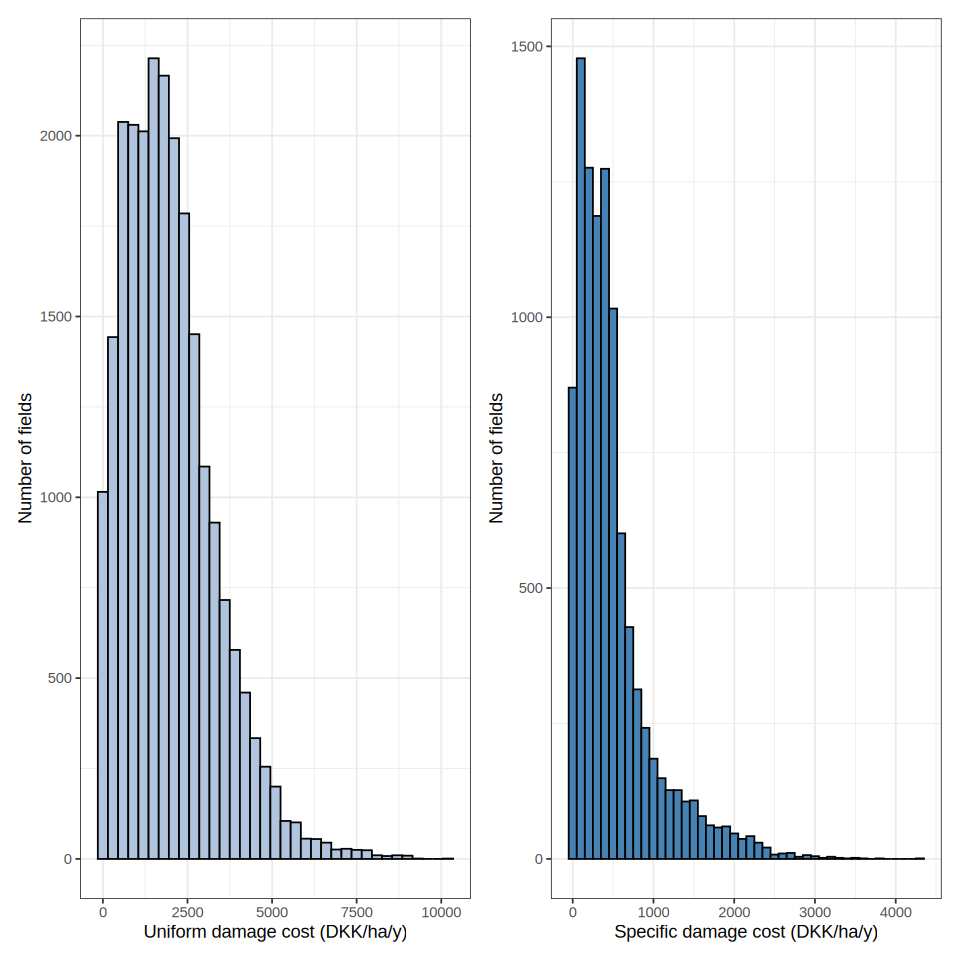
\includegraphics[width=0.8\textwidth]{figures/hist_uniform_specific_total.png}
\caption{Total Distribution of Uniform Damage Cost (DKK/ha/y) (left figure); and Specific Damage Cost (DKK/ha/y)(right figure) }
\label{fig:hist_DC_allfields}
\end{figure}


Distributions for both the specific and the uniform valuation approach are markedly right-skewed, with the majority of fields concentrated at relatively lower damage costs and a long tail of high-cost fields. 
With the uniform approach, the distribution is shifted rightward relative to the specific approach, reflecting the higher uniform damage cost estimate. 
The range of damage costs across fields is substantial in both approaches, ranging from approximately 0-10.000 DKK/ha under the uniform approach and from 0-4400 DKK/ha under the specific valuation approach -  underlining that individual fields differ considerably in the environmental burden they impose on receiving water bodies.

This heterogeneity is obscured in catchment-level averages. It is, however, precisely this extensive variation, that motivates the field-level approach adopted in this thesis: fields within the tail impose a disproportionately large environmental cost and would be indistinguishable from low-cost fields under a spatially undifferentiated regulatory framework. Field level variations in damage costs within the individual 11 catchments are reported in Appendix~\ref{Field-level Distribution of Damage Costs}


\subsubsection{Robustness Check: Spring Barley with Catch Crop}

\begin{table}[H]
\centering
\small
\caption{Area-weighted average damage costs (DKK/ha/y): Winter Wheat vs Spring Barley
Leaching Reference}
\label{tab:sensitivity_all}
\resizebox{\textwidth}{!}{%
\begin{tabular}{lcccc}
\toprule
& \multicolumn{2}{c}{\textbf{Specific Damage Cost (DKK/ha/y)}}
& \multicolumn{2}{c}{\textbf{Uniform Damage Cost (DKK/ha/y)}} \\
\cmidrule(lr){2-3} \cmidrule(lr){4-5}
\textbf{Catchment} & \textbf{Winter Wheat} & \textbf{Spring Barley} & \textbf{Winter Wheat} & \textbf{Spring Barley} \\
& & \textbf{w. Catch Crop} & & \textbf{w. Catch Crop} \\
\midrule
Lister Dyb                    & ---   & ---   & 1,293.8 &   641.5 \\
Nissum Bredning               & ---   & ---   & 2,371.0 & 1,100.2 \\
Nissum Fjord, Felsted Kog     & 250.9 & 124.5 & 2,325.3 & 1,153.9 \\
Thisted Bredning              & ---   & ---   & 2,515.3 & 1,184.9 \\
Nibe Bredning og Langerak     & ---   & ---   & 2,576.1 & 1,219.2 \\
Randers Fjord, indre          & 314.9 & 153.3 & 1,595.0 &   776.4 \\
Horsens Fjord, indre          & 1,649.3 & 832.9 & 2,086.4 & 1,053.6 \\
Odense Fjord, Seden Strand    & 731.6 & 390.5 & 1,845.3 &   984.9 \\
Isefjord, indre               & 1,104.7 & 636.5 & 1,769.6 & 1,019.5 \\
Karrebæk Fjord                & ---   & ---   & 1,672.8 & 1,029.3 \\
Roskilde Fjord, indre         & 679.0 & 446.7 & 1,013.7 &   666.9 \\
\bottomrule
\end{tabular}%
}
\begin{tablenotes}
\footnotesize
\item \textit{Notes:} All values measured in DKK per hectare per year, weighted by
area. Specific refers to location-specific damage costs; Uniform refers to the EU average damage cost of 130.76 DKK/kg N. `---' indicates that specific damage cost estimates are unavailable for this catchment.
\end{tablenotes}
\end{table}

Table~\ref{tab:sensitivity_all} compares area-weighted average damage costs (DKK/ha) under the winter wheat reference scenario and the alternative scenario based on spring barley with a catch crop (Section~\ref{Leaching Map for Continuous Winter Wheat and Spring Barley}), for both the specific and uniform valuation approaches. 
The purpose is to assess whether the spatial patterns in damage costs identified in the preceding sections are robust to the choice of reference crop.

As expected, damage costs are substantially lower under the spring barley with catch crop scenario across all catchments and both valuation approaches. 
The reduction reflects the nitrogen-binding effect of the catch crop, which reduces leaching from the root zone and consequently lowers nitrogen loads to coastal waters. 

Under the specific approach, the proportional reduction in average damage costs (DKK/ha) ranges from 42 to 51 percent across most catchments, with Roskilde Fjord, indre as a notable outlier at 34 percent -- the smallest relative reduction under both valuation approaches. 

A similar pattern holds under the uniform approach, where the majority of catchments cluster around a 50 percent reduction in average damage costs moving from the winter wheat scenario to the spring barley scenario. 


Importantly, the relative ranking of catchments is largely preserved across the two scenarios. 
Under the specific approach, the ranking is stable at both ends --- Horsens Fjord, indre and Isefjord, indre consistently displays the highest damage costs and Nissum Fjord, Felsted Kog and Randers Fjord, indre remain at the lower end --- though some reshuffling occurs in the middle of the distribution, with for example Odense Fjord, Seden Strand overtaking Roskilde Fjord, indre under the spring barley scenario. 

Under the uniform approach, the top and bottom of the distribution are similarly stable, with Nibe Bredning og Langerak an Thisted Bredning retaining their position at the top, though distributions are largely preserved, some reshuffling does occur. These changes in relative average damage costs between catchments may partly reflect differences in spatial resolution between the two leaching reference maps (Section~\ref{Leaching Map for Continuous Winter Wheat and Spring Barley}).


Overall, this suggests that the spatial patterns in damage costs are driven primarily by underlying biophysical characteristics --- soil type, retention capacity, drainage, and proximity to vulnerable water bodies --- rather than by the specific cropping assumption. The reference scenario therefore appears somewhat robust as a basis for spatial targeting at the catchment level, even if the absolute level of damage costs is sensitive to crop choice. However, given differences in spatial resolution between the two leaching maps and the absence of a field-level evaluation, this robustness check should be considered indicative at best rather than conclusive --- whether the results extend to the field level and to a broader set of reference crop rotations warrants further investigation.
 

\subsubsection{Robustness Check: Crop Choice effects on Damage Cost Distribution}


\begin{table}[H]
\centering
\small
\caption{Area-weighted average damage cost in DKK/ha/y by crop type actually
cultivated, under the winter wheat reference scenario.}
\label{tab:dc_crop_short}
\resizebox{\textwidth}{!}{%
\begin{tabular}{lcccc}
\toprule
& \multicolumn{2}{c}{\textbf{Uniform Damage Cost (DKK/ha/y)}}
& \multicolumn{2}{c}{\textbf{Specific Damage Cost (DKK/ha/y)}} \\
\cmidrule(lr){2-3} \cmidrule(lr){4-5}
\textbf{Catchment} & \textbf{W. Wheat} & \textbf{S. Barley}
                   & \textbf{W. Wheat} & \textbf{S. Barley} \\
\midrule
Lister Dyb                   & 1,263 & 1,293 & ---     & ---     \\
Nissum Bredning              & 2,237 & 2,377 & ---     & ---     \\
Nissum Fjord, Felsted Kog    & 2,499 & 2,208 &   270 &   238 \\
Thisted Bredning             & 2,416 & 2,622 & ---     & ---     \\
Nibe Bredning og Langerak    & 2,807 & 2,591 & ---     & ---     \\
Randers Fjord, indre         & 1,743 & 1,661 &   344 &   328 \\
Horsens Fjord, indre         & 2,164 & 2,154 & 1,711 & 1,703 \\
Odense Fjord, Seden Strand   & 1,899 & 1,747 &   753 &   693 \\
Isefjord, indre              & 1,638 & 2,016 & 1,022 & 1,258 \\
Karrebæk Fjord               & 1,664 & 1,681 & ---     & ---     \\
Roskilde Fjord, indre        &   980 & 1,032 &   656 &   691 \\
\bottomrule
\end{tabular}%
}
\begin{tablenotes}
\footnotesize
\item \textit{Notes:} All values measured in DKK per hectare per year, weighted by
area. Each column shows damage costs for fields where the respective crop was actually
cultivated in 2024, evaluated under the winter wheat reference scenario. `---' indicates
that specific damage cost estimates are unavailable for this catchment.
W.~Wheat = Winter Wheat; S.~Barley = Spring Barley.
\end{tablenotes}
\end{table}

The winter wheat reference scenario represents a counterfactual land use assumption in which all fields are hypothetically cultivated with winter wheat. This provides a consistent basis for comparing field-level damage potential by holding land use constant and isolating biophysical differences in nitrogen leaching and retention.



A limitation of this approach is that it abstracts from actual crop allocation decisions, which may influence realized nitrogen losses. If crop choices are systematically aligned with environmental vulnerability --- for instance if less leaching-intensive crops are preferentially allocated to more environmentally sensitive fields --- then observed land use patterns would partly reflect endogenous environmental adaptation. In that case, estimates based on a uniform reference crop could overstate true spatial differences in damage potential.

Table~\ref{tab:dc_crop_short} presents area-weighted average damage costs under the 
winter wheat reference scenario for fields actually cultivated with winter wheat and 
spring barley in 2024. 

The results show no apparent systematic pattern in damage costs across crop categories. Spring barley fields exhibit higher damage costs than winter wheat fields in some catchments and lower in others, with no consistent pattern across catchments or valuation approaches. This absence of systematic sorting is confirmed by the full crop-category results reported in Appendix~\ref{app:field-level-damage-costs} and suggests that crop allocation is driven by factors other than environmental burden (e.g.\ yield potential).

This lack of systematic crop sorting supports the use of a standardized reference scenario. 
If farmers systematically allocated crops based on environmental burden, observed crop distributions would introduce a systematic bias into estimated damage costs.




Taken together, the results in this section suggest two main findings. First, nitrogen damage costs vary substantially across catchments and fields, reflecting differences in leaching potential and retention capacity, while the choice of valuation approach affects the absolute level of damage costs and the relative ranking of catchments. Second, the spatial pattern across catchments appears robust to the choice of reference crop, as the relative ranking is largely preserved across both scenarios examined. 
Furthermore, the absence of systematic crop sorting across fields with differing damage cost potential supports the use of a standardised reference scenario, suggesting that observed crop allocation is driven primarily by agronomic rather than environmental considerations. 
However, as both robustness analyses are conducted at the catchment level only, these conclusions should be considered indicative rather than conclusive at the field level, and so should be evaluated in more detail.

\subsection{Field-Level Profitability from Society's Perspective}
\label{sec:society-profitability}

This section presents field-level profitability from society's perspective under the winter wheat reference scenario. 
Catchment-level results are presented first under the specific valuation approach, followed by the uniform valuation approach. Field-level distributions are then analysed to assess within-catchment variation in social profitability. For the interested reader, results under the spring barley scenario are presented in Appendix~\ref{Profitability from the perspective of society - Spring Barley Reference}.


\subsubsection{Average Catchment Level Profitability from the Perspective of Society}

\paragraph{The Specific Valuation Approach} Table~\ref{tab:dbii-vinterhvede-specific} reports average field-level profitability from society's perspective under the catchment-specific damage cost approach. $\mathrm{DBII^{farmer}}$ is included in the table for comparison. 

\begin{table}[H]
\centering
\small
\caption{Average profitability from society's perspectives (DKK/ha/year) based on specific damage costs under the winter wheat scenario.}
\label{tab:dbii-vinterhvede-specific}
\resizebox{\textwidth}{!}{
\begin{threeparttable}
\begin{tabular}{lrrrrrr}
\toprule
\textbf{Catchment} & \textbf{Fields} & \boldmath$\textcolor{red}{\mathbf{DBII^{farmer}}}$ & \boldmath$\mathbf{DBII^{society}}$ & \textbf{Fine} &
\textbf{Coarse} & \textbf{Loamy} \\
\midrule
Nissum Fjord, Felsted Kog  & 2,916 & $-$1,238 & $-$1,476 & $-$1,371 (732) & $-$1,147 (573) & $-$1,634 (1,611) \\
Randers Fjord, indre       & 4,094 &    783   &    466   &    670 (1,029) &    226 (594)   &    434 (2,471) \\
Horsens Fjord, indre       &   674 &     86   & $-$1,567 & $-$1,429 (166) & $-$2,348 (90)  & $-$1,479 (418) \\
Odense Fjord, Seden Strand &   985 &  1,637   &    895   &    856 (220)   &    252 (127)   &  1,012 (638) \\
Isefjord, indre            &   577 &  1,597   &    539   &  1,540 (134)   & $-$ (56)       &    220 (387) \\
Roskilde Fjord, indre      &   245 &  1,304   &    811   &    416 (50)    & $-$ (35)       &    935 (160) \\
\addlinespace\bottomrule
\end{tabular}
\begin{tablenotes}
\footnotesize
\item \textit{Notes:} All values are measured in DKK per hectare and weighted by area.
$\mathrm{DBII^{farmer}}$ denotes profitability from the farmer's perspective excluding environmental externalities and is inserted for comparability, while $\mathrm{DBII^{society}}$ denotes profitability net of catchment-specific nitrogen damage costs. 
Fine, Coarse, and Loamy refer to average social profitability for fields on the respective soil type within each catchment; numbers in parentheses indicate the number of fields. `$-$' indicates missing values or fewer than 20 fields and is therefore not reported.
\end{tablenotes}
\end{threeparttable}
}
\end{table}

Under the specific valuation approach, four catchments exhibit positive $\mathrm{DBII^{society}}$: Odense Fjord, Seden Strand (+895 DKK/ha),  Roskilde Fjord, indre (+811 DKK/ha), Isefjord, indre (+539 DKK/ha), and Randers Fjord, indre (+466 DKK/ha). In contrast, Nissum Fjord, Felsted Kog ($-$1,476 DKK/ha) and Horsens Fjord, indre ($-$1,567 DKK/ha) display negative social profitability. 
The range in $\mathrm{DBII^{society}}$ spans 2,462 DKK/ha, highlighting substantial spatial variation across catchments in 2024.




\begin{table}[H]
\centering
\small
\caption{Change in field-level profitability from the farmer's to society's perspective (DKK/ha/year) under the specific damage cost approach (winter wheat scenario).}
\label{tab:dbii-change-specific}
\begin{threeparttable}

\begin{tabular}{lrrrrr}
\toprule
\textbf{Catchment} & \boldmath$\Delta$ \textbf{DBII} &
\textbf{Fine} & \textbf{Coarse} & \textbf{Loamy} \\
\midrule\addlinespace

Nissum Fjord, Felsted Kog  & $-$238  & $-$245 & $-$235 & $-$251 \\
Randers Fjord, indre       & $-$317  & $-$306 & $-$303 & $-$315 \\
Horsens Fjord, indre       & $-$1,653 & $-$1,669 & $-$1,714 & $-$1,629 \\
Odense Fjord, Seden Strand & $-$742  & $-$735 & $-$739 & $-$731 \\
Isefjord, indre            & $-$1,058 & $-$1,152 & $-$\; & $-$1,090 \\
Roskilde Fjord, indre      & $-$493  & $-$615 & $-$\;  & $-$634 \\
\addlinespace\bottomrule
\end{tabular}


\begin{tablenotes}
\footnotesize
\item \textit{Notes:} $\Delta$ DBII is defined as $\mathrm{\text{DBII}^{Society}} - \mathrm{\text{DBII}^{Farmer}}$ under the specific damage cost approach. 
Positive values indicate an increase in profitability when environmental externalities are internalised, while negative values indicate a reduction. 
Soil-type changes are computed as the difference in average profitability between social and farmer perspectives for each soil type within each catchment. `$-$' indicates missing values or fewer than 20 observations.
\end{tablenotes}

\end{threeparttable}
\end{table}

The differences between farmer's and society's field-level profitability are reported in Table~\ref{tab:dbii-change-specific}. 
The results show considerable heterogeneity in the effect of internalising catchment-specific nitrogen damage costs. 
The largest downward adjustment is observed in Horsens Fjord, indre, where average profitability declines by 1,653 DKK/ha relative to $\mathrm{DBII^{farmer}}$, shifting from a slightly positive (86 DKK/ha) to a strongly negative profitability ($-$1,567 DKK/ha).

By comparison, Randers Fjord, indre experiences a relatively modest adjustment of $-$317 DKK/ha and remains on average profitable despite only having only moderate $\mathrm{DBII^{farmer}}$. 
Similarly, Nissum Fjord, Felsted Kog exhibits the smallest adjustment among the six catchments (238 DKK/ha), yet remains among the on average least profitable from both the farmer's and society's perspectives due to its already low $\mathrm{DBII^{farmer}}$. 


The change in field-level profitability across soil types (Table~\ref{tab:dbii-change-specific}) also warrants attention.
At first glance, the absence of a systematic relationship between soil type and $\mathrm{DBII^{social}}$ may appear counterintuitive. 
From an agronomic perspective, coarse-sandy soils would generally be expected to exhibit higher nitrogen leaching rates and, consequently, higher environmental damage costs than loamy soils.

However, in the winter wheat scenario, nitrogen losses are modeled under norm-based fertiliser constraints (Section \ref{sec:The Winter Wheat Reference Scenario}). 
Because permitted nitrogen application rates differ by soil type --- with loamy soils generally allowed higher fertiliser inputs than fine and coarse sandy soils --- 
nitrogen leaching under the reference scenario reflects not only soil properties, but also regulatory input restrictions embedded in the fertilisation norms. 
This likely explains why no clear relationship between soil type and environmental damages is observed.

Overall, the results demonstrate that neither field-level profitability from the farmer's perspective nor catchment-specific nitrogen damage costs are sufficient indicators of field-level profitability from society's perspective under the specific valuation approach. 
Field-level profitability from society's perspective reflects the combined effect of the two components, and the relative importance of each varies across catchments. 
Consequently, assessments based solely on profitability from the farmer's perspective or solely on environmental damages may incorrectly identify which catchments impose the greatest social costs. 


\paragraph{The Uniform Valuation Approach}

Table~\ref{tab:dbii-vinterhvede-uniform} presents field-level profitability from society's perspective under the uniform damage cost approach. $\mathrm{DBII^{farmer}}$ is included in the table for comparison.


\begin{table}[H]
\centering
\small
\caption{Average field-level profitability from farmer's and society's perspectives (DKK/ha/year) based on uniform damage costs under the winter wheat scenario.}
\label{tab:dbii-vinterhvede-uniform}
\resizebox{\textwidth}{!}{
\begin{threeparttable}
\begin{tabular}{lrrrrrrr}
\toprule
\textbf{Catchment} & \textbf{Fields} & \boldmath$\textcolor{red}{\mathbf{DBII^{farmer}}}$ & \boldmath$\mathbf{DBII^{society}}$ &
\textbf{Fine} & \textbf{Coarse} & \textbf{Loamy} \\
\midrule\addlinespace
Lister Dyb                 & 4,498 & $-$74    & $-$1,382 & $-$1,850 (1,154) & $-$1,266 (761)  & $-$1,208 (2,583) \\
Nissum Bredning            & 1,098 & $-$2,071 & $-$4,464 & $-$3,138 (268)   & $-$ (154)       & $-$4,965 (676)   \\
Nissum Fjord, Felsted Kog  & 2,916 & $-$1,238 & $-$3,512 & $-$3,393 (732)   & $-$3,085 (573)  & $-$3,710 (1,611) \\
Thisted Bredning           & 1,146 & $-$4     & $-$2,563 & $-$3,094 (310)   & $-$3,649 (155)  & $-$2,173 (681)   \\
Nibe Bredning og Langerak  & 4,734 & 621      & $-$1,949 & $-$1,963 (1,563) & $-$2,517 (636)  & $-$1,833 (2,535) \\
Randers Fjord, indre       & 4,094 & 783      & $-$799   & $-$576 (1,029)   & $-$1,007 (594)  & $-$844 (2,471)   \\
Horsens Fjord, indre       &   674 & 86       & $-$2,003 & $-$1,871 (166)   & $-$2,803 (90)   & $-$1,911 (418)   \\
Odense Fjord, Seden Strand &   985 & 1,637    & $-$220   & $-$263 (220)     & $-$873 (127)    & $-$101 (638)     \\
Isefjord, indre            &   577 & 1,597    & $-$126   & 846 (134)        & $-$ (56)        & $-$436 (387)     \\
Karrebæk Fjord             & 1,069 & 2,274    & 607      & 650 (256)        & $-$88 (137)     & 692 (676)        \\
Roskilde Fjord, indre      &   245 & 1,304    & 501      & 113 (50)         & $-$ (35)        & 623 (160)        \\
\addlinespace
\bottomrule
\end{tabular}
\begin{tablenotes}
\footnotesize
\item \textit{Notes:} All values are measured in DKK per hectare and weighted by area. 
$\mathrm{DBII^{farmer}}$ denotes private profitability excluding environmental externalities, 
while $\mathrm{DBII^{society}}$ denotes profitability net of uniform nitrogen damage costs (130.8 DKK/kg N). 
Fine, Coarse, and Loamy refer to average social profitability for fields on the respective soil type within each catchment; numbers in parentheses indicate the number of fields. `$-$' indicates missing values or fewer than 20 fields and is therefore not reported.
\end{tablenotes}
\end{threeparttable}
}
\end{table}


Compared to the specific approach profitability from the perspective of society is substantially lower across almost all catchments. 
This reflects the fact that the uniform damage cost estimate of 130.76 DKK/kg N exceeds the catchment-specific estimate in all 6 catchments where specific values are available.

Under the uniform approach, only two catchments retain positive $\mathrm{DBII^{society}}$: Karrebæk Fjord (+607 DKK/ha) and Roskilde Fjord, indre (+501 DKK/ha). 
All remaining catchments exhibit negative average values, ranging from $-$126 DKK/ha in Isefjord, indre to $-$4,464 DKK/ha in Nissum Bredning. 
The overall difference across catchments exceeds 5,000 DKK/ha, indicating substantial spatial heterogeneity in social profitability.

The west–--east gradient observed under $\mathrm{DBII^{farmer}}$ is still partly visible under the uniform approach, though less pronounced. 

The relative changes ($\Delta$) between $\mathrm{DBII^{society}}$ and $\mathrm{DBII^{farmer}}$ are reported in Table~\ref{tab:dbii-change-uniform}. 


\begin{table}[H]
\centering
\small
\caption{Change in profitability from farmer's to society's perspective (DKK/ha/year) under uniform damage costs in the winter wheat scenario.}
\label{tab:dbii-change-uniform}
\begin{threeparttable}
\begin{tabular}{lrrrrr}
\toprule
\textbf{Catchment} & \textbf{Fields} & \boldmath$\Delta$ \textbf{DBII} & \textbf{Fine} & \textbf{Coarse} & \textbf{Loamy} \\
\midrule\addlinespace
Lister Dyb                 & 4,498 & $-$1,308 & $-$1,349 & $-$1,288 & $-$1,297 \\
Nissum Bredning            & 1,098 & $-$2,393 & $-$2,481 & $-$ & $-$2,296 \\
Nissum Fjord, Felsted Kog  & 2,916 & $-$2,274 & $-$2,267 & $-$2,173 & $-$2,327 \\
Thisted Bredning           & 1,146 & $-$2,559 & $-$2,564 & $-$2,494 & $-$2,462 \\
Nibe Bredning og Langerak  & 4,734 & $-$2,570 & $-$2,520 & $-$2,684 & $-$2,562 \\
Randers Fjord, indre       & 4,094 & $-$1,582 & $-$1,552 & $-$1,233 & $-$1,593 \\
Horsens Fjord, indre       &   674 & $-$2,089 & $-$2,111 & $-$2,169 & $-$2,061 \\
Odense Fjord, Seden Strand &   985 & $-$1,857 & $-$1,854 & $-$1,864 & $-$1,844 \\
Isefjord, indre            &   577 & $-$1,723 & $-$1,846 & $-$ & $-$1,746 \\
Karrebæk Fjord             & 1,069 & $-$1,667 & $-$1,703 & $-$1,655 & $-$1,670 \\
Roskilde Fjord, indre      &   245 & $-$803   & $-$918   & $-$ & $-$946 \\
\addlinespace
\bottomrule
\end{tabular}
\begin{tablenotes}
\footnotesize
\item \textit{Notes:} $\Delta DBII$ is defined as $\mathrm{DBII^{society}} - \mathrm{DBII^{farmer}}$ under uniform nitrogen damage costs (130.8 DKK/kg N). Fine, Coarse, and Loamy show the corresponding change in average profitability for each soil type within each catchment. `$-$` indicates fewer than 20 fields and is therefore not reported.
\end{tablenotes}
\end{threeparttable}
\end{table}


The changes under the uniform damage cost approach show a consistent downward adjustment in profitability when moving from the farmer’s to society's perspective across all catchments. 
The magnitude of the reduction in DBII varies, with the largest declines observed in Nibe Bredning og Langerak ($-$2,570 DKK/ha) and Thisted Bredning ($-$2,559 DKK/ha), while Roskilde Fjord, indre exhibits the smallest reduction ($−$803 DKK/ha). 

Taken together, the results show that $\mathrm{DBII^{society}}$ under the uniform approach is driven by the interaction between  $\mathrm{DBII^{farmer}}$ and spatial variation in nitrogen leaching, while the per unit damage cost is held constant across catchments.

Compared to the specific valuation approach, this implies a more mechanically determined spatial pattern, where catchments with higher nitrogen losses are penalised proportionally more, but where substantial variation in $\mathrm{DBII^{farmer}}$ continues to shape the overall distribution of social outcomes --- At least for the catchments considered here. 
 
In this sense, the uniform approach compresses rather than reshuffles the ranking: catchments with high nitrogen losses are penalised more heavily, but the underlying spatial structure from $\mathrm{DBII^{farmer}}$ somewhat persists.



\subsubsection{Field Level Profitability From the Perspective of Society}


\paragraph{The Specific Valuation Approach}

\begin{figure}[H]
\centering
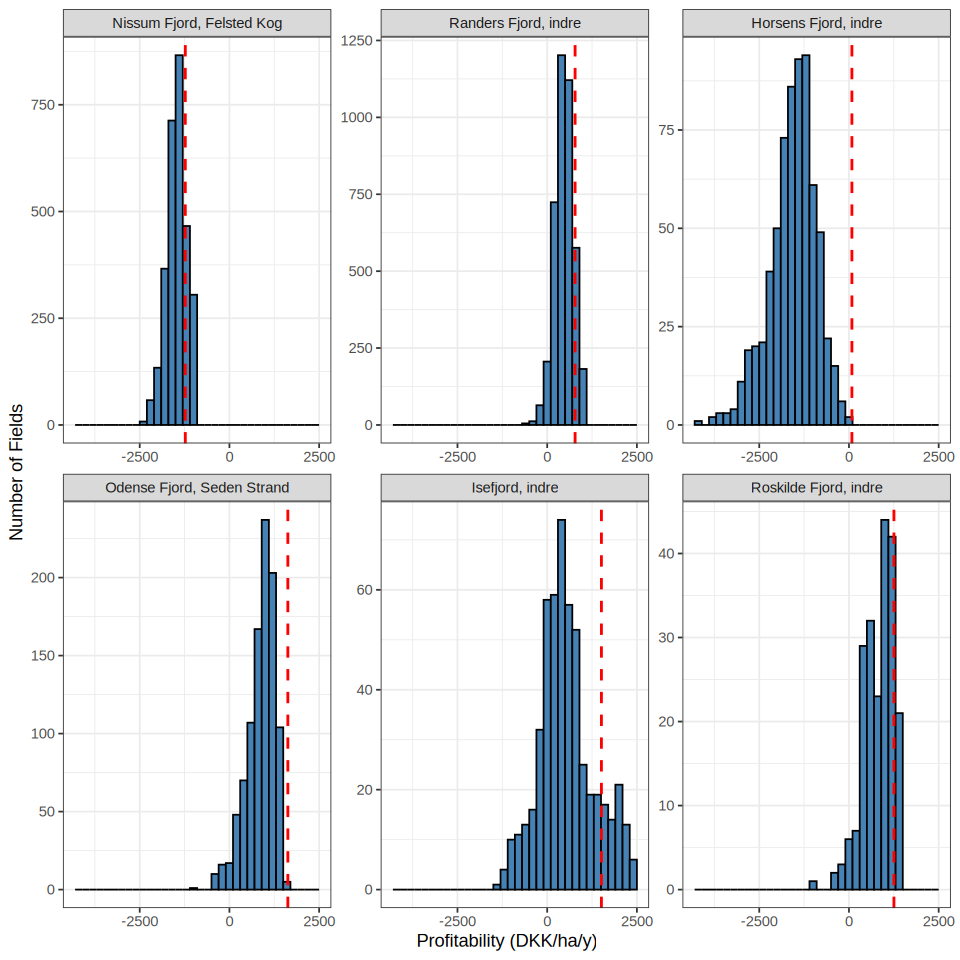
\includegraphics[width=0.8\textwidth]{figures/hist_specific_DBII_hvede.png}
\caption{Distribution of Field-Level Profitability from Society's Perspective (DKK/ha/y). The Specific Valuation Approach. Red dashed line $=$ average field-level profitability (winter wheat reference)}
\label{fig:social-dbii-specific-hvede}
\end{figure} 


Figure~\ref{fig:social-dbii-specific-hvede} presents the field-level distribution of $\mathrm{DBII^{society}}$ across the six catchments for which specific damage cost estimates are available. 
The red dashed lines indicate the average field-level profitability for winter wheat within each catchment, enabling a direct visual comparison between $\mathrm{DBII^{farmer}}$ specific to the catchment and $\mathrm{DBII^{society}}$ at the field level.

The leftward shift from the reference line to the centre of each distribution reflects the average catchment-specific damage costs, and its magnitude varies considerably across catchments. 
In Horsens Fjord, indre the gap is by far the largest —-- consistent with the high catchment-specific damage cost --- shifting the distribution well into negative territory despite a near-zero $\mathrm{DBII^{farmer}}$. In Nissum Fjord, Felsted Kog, the shift is more modest, but the distribution is nevertheless entirely in negative territory, driven primarily by already low private economic returns rather than by elevated damage costs.

The remaining four catchments display positive $\mathrm{DBII^{society}}$. 
For Randers Fjord, indre, Odense Fjord, Seden Strand and Roskilde Fjord, indre, the vast majority of fields are socially profitable, with only a limited share falling below zero. Isefjord, indre stands out among these with a wider and flatter distribution, where a notable share of fields display negative $\mathrm{DBII^{society}}$ despite a positive catchment average (i.e., red line).



\paragraph{The Uniform Valuation Approach}


\begin{figure}[H]
\centering
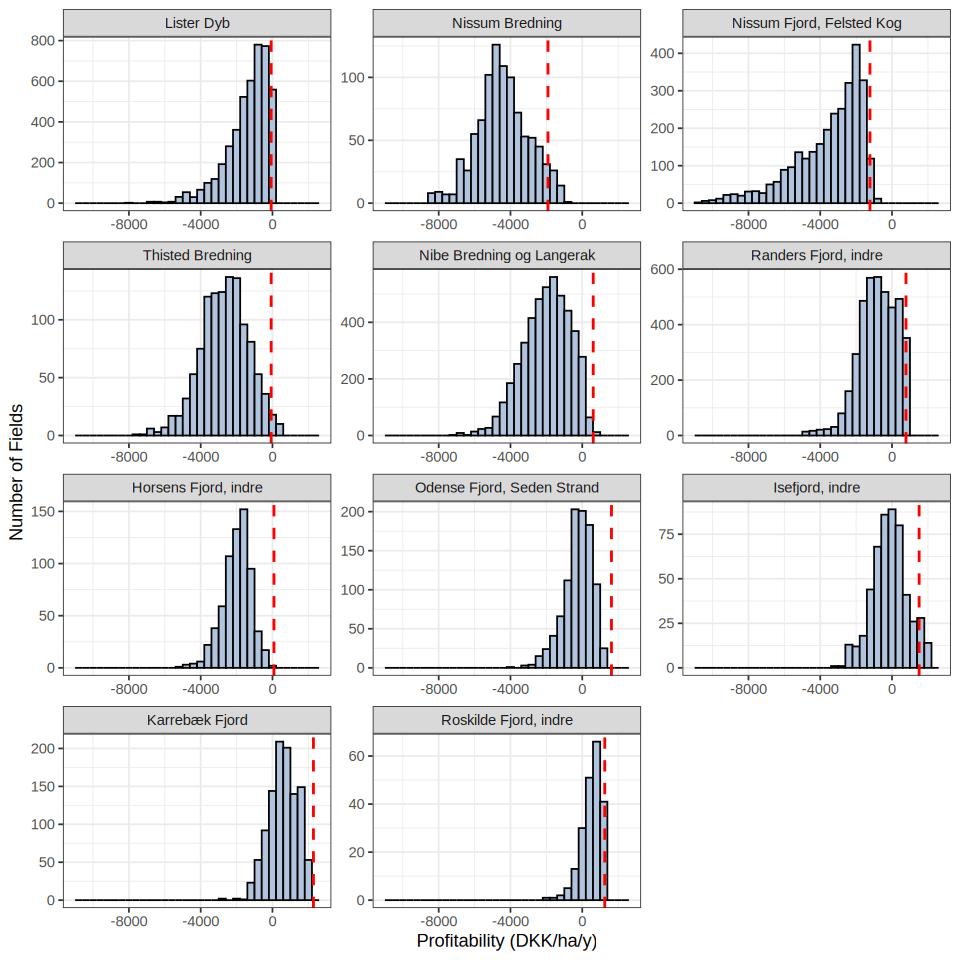
\includegraphics[width=0.8\textwidth]{figures/hist_uniform_DBII_hvede.png}
\caption{Distribution of Profitability from Society's Perspective (DKK/ha/y). Uniform Valuation Approach. Red dashed line $=$ average field-level profitability (winter wheat reference)}
\label{fig:social-dbii-uniform-hvede}
\end{figure} 


Figure~\ref{fig:social-dbii-uniform-hvede} presents the field-level distribution of $\mathrm{DBII^{society}}$ under the uniform valuation approach across all eleven catchments. 
The red dashed line indicates the area-weighted $\mathrm{DBII^{farmer}}$ of winter wheat within each catchment.

The most striking feature relative to the specific approach is the pronounced leftward shift of all distributions -- a direct consequence of the higher uniform damage cost (130.8 DKK/kg N). 
Whereas several catchments retained positive $\mathrm{DBII^{society}}$ for the majority of fields under the specific approach, the distributions under the uniform approach are predominantly centered in negative territory across almost all catchments. 
Only Karrebæk Fjord and Roskilde Fjord, indre display distribution centres to the right of zero, consistent with their positive $\mathrm{DBII^{society}}$ --- while the reference line remains positive across the majority of catchments, illustrating the extent to which the uniform damage cost erodes private economic returns.

The gap between the $\mathrm{DBII^{farmer}}$ reference line and the distribution center is determined by the amount of nitrogen leaching to the coastal waters, rather than by heterogeneous damage valuations. This is most visible in the western and northern catchments, where the distributions of Nissum Bredning, Nissum Fjord, Felsted Kog, Thisted Bredning, and Nibe Bredning og Langerak are shifted furthest into negative territory.

Across all catchments, substantial within-catchment heterogeneity persists. 
As under the specific approach, catchment distributions generally contains both fields where private economic returns exceed environmental costs -- representing a net gain to society from continued production -- and fields where damage costs substantially exceed private returns. 
Under the uniform approach, however, the latter group is considerably larger, and only the right tails of catchments such as Karrebæk Fjord, Roskilde Fjord, indre, Odense Fjord, Seden Strand and Isefjord, indre identify fields that remain socially profitable.

This within-catchment heterogeneity observed both when applying the uniform and the specific damage cost estimates, is the central motivation for a field-level approach. Catchment averages obscure the fact that each distribution contains both fields where private economic returns are high relative to environmental costs -- representing a net gain to society from continued production -- and fields where damage costs substantially exceed private economic returns, representing the strongest candidates for targeted land retirement. 
Identifying and distinguishing between these two groups is of primary interest to society.

However, under the specific approach, four catchments retain positive $\mathrm{DBII^{society}}$ , and within these, the majority of individual fields are socially profitable. 
Under the uniform approach, this group narrows considerably -- only Karrebæk Fjord and Roskilde Fjord, indre retain positive averages, and the share of socially profitable fields is substantially reduced across all catchments. 
The choice of valuation approach therefore has direct implications for which fields would be identified as candidates for continued production versus targeted intervention. 
Fields that appear socially profitable under the specific approach may be classified as socially unprofitable under the uniform approach -- underscoring that the spatial targeting of land-use policy is sensitive not only to the distribution of field-level profitability from farmer's perspective and nitrogen losses, but also, indeed, to the underlying damage cost valuation approach. 

This is an important result, as it demonstrates that conclusions regarding the field-level profitability from society's perspective are highly sensitive to how damage cost are specified. 
The findings therefore highlight the importance of the underlying assumptions and suggest a need for further work on improving the robustness and empirical basis of damage-cost estimates.




%This is an important result, as it demonstrates that conclusions regarding the social profitability of agricultural production are highly sensitive to the assumed damage costs of nitrogen emissions. The findings therefore underscore the need for the development of more robust and well-founded damage-cost estimates. However, although the damage cost estimates applied here are highly uncertain, the cost of nitrogen loads in coastal waters is clearly not zero. This implies that, despite the uncertainty, using even conservative or lower-bound estimates is preferable to excluding damage costs altogether, as doing so would effectively assign a zero value to nitrogen pollution and thereby risk systematically underestimating its social costs.


\section{Limitations}
\label{sec:Limitations}

This section provides a structured overview of the main limitations of the analysis. 
Several limitations are inherent to the pilot nature of the study and reflect constraints in data availability, sample coverage, and methodological choices made. 
The most substantive of these -- relating to the allocation model, the use of a standardised reference scenario, the reliance on average DBII estimates and the damage cost estimates -- are discussed in greater depth in Section~\ref{sec:discussion}.

\subsection{Data Limitations}

\paragraph{Single year (2024).}
The analysis is based on a single year of accounting data from 2024, characterised by excessive rainfall and below-normal yields across all major crops. 
This limits the generalisability of the results, as estimated field-level profitability reflects year-specific conditions rather than long-run productive potential, and structural differences in productivity cannot be disentangled from local weather effects.


\paragraph{Limited sample size.}
The sample covers 894 conventional farms corresponding to 23,336 fields across 11 catchments. 
The sample may not be representative of all crop--soil type combinations, particularly for less common crops. 
The analysis is geographically restricted to 11 coastal catchments, and results should not be directly generalised to other catchments.


\paragraph{Self-selection bias.}
Participation in the SEGES Financial Database is voluntary, introducing a risk of self-selection bias as participating farms may systematically differ from non-participating farms. 
Participating farms may therefore not be representative of the broader farm population in terms of size, productivity, and management practices.


\paragraph{Self-Reported Data.}Differences in inventory handling and accounting practices may affect comparability across farms. While individual entries cannot be independently verified, the data have undergone validation by SEGES prior to inclusion. It is assumed that Farmers report accurately and in accordance with standard accounting practices.

% \paragraph{Self-reported data.} Differences in inventory handling and accounting practices may affect comparability across farms. The data have undergone validation by SEGES prior to inclusion. Although more detailed sub-items and supplementary information are available in the farm accounts, the sub-items do not align one-to-one with the aggregate cost items for two reasons: (1) Farmers are not required to report at the sub-item level, meaning the supplementary data largely reflects individual accounting practices rather than a standardized reporting structure; and (2) Certain sub-items may be absent, as they were not deemed relevant for data collection by SEGES. Since reporting at a detailed level is not mandatory, the aggregate cost items provide the most consistent and comparable basis for analysis.

\paragraph{Timing of Purchases and Sales.}
Input and output variables are measured as aggregate changes in the accounting balance during the financial year of 2024.\footnote{Account balance $=$ closing inventory $+$ cash turnover $+$ internal turnover $-$ opening inventory.}The timing of purchases and sales may introduce variability in recorded inputs and outputs. 
For example, for inputs such as fertiliser, seasonal price fluctuations and inventory carryover can affect costs recorded for the planning period, while crop revenues depend on the timing of sales as market prices vary throughout the year. Within the scope of this thesis, we have assumed constant prices.


% \paragraph{Leaching estimates for stylised cropping systems only.} 
% Detailed nitrogen leaching estimates are available only for two stylised cropping systems: winter wheat and spring barley. 
% Leaching maps for other crop rotations are not available, precluding estimation of realised field-level nitrogen losses based on observed crop rotations.


\subsection{Methodological Limitations}

\paragraph{Aggregation of soil types. }
Soil types are aggregated into three broad categories, reducing granularity and potentially obscuring finer soil--yield relationships.

\paragraph{Field-level heterogeneity.}
Beyond soil type and crop, profitability is likely influenced by factors such as field size, shape, and climate \citep{olsen2017} -- characteristics not captured in the current model.

\paragraph{Average field-level profitability by catchment and soil type.} All fields within the same catchment--soil type combination are assigned identical profitability estimates, ignoring within-group heterogeneity. 

\paragraph{Reference scenario.}
All fields are evaluated under a standardised winter wheat scenario with regulatory fertilisation norms. 
Estimates reflect potential rather than realised nitrogen losses.

\paragraph{Spatial resolution.}
Both leaching and retention are model-based estimates and may not fully capture actual conditions at the individual field level, introducing some imprecision in field-level variation.


\subsection{Damage Cost Limitations}

\paragraph{Limited availability of specific damage cost estimates.} 
Location-specific estimates are available for only six of eleven coastal catchments in Denmark. 

\paragraph{Partial and dated damage cost estimates.} Location-specific estimates from \citet{andersen2019} capture only recreational and amenity values and property prices, and should be interpreted as lower-bound measures of total environmental costs. The uniform ENA estimates from \citet{brink2011} cover a broader range of categories but represent an EU-wide average rather than a national valuation. Both sets of estimates are based on dated 
baselines --- 2010 for location-specific and 2005 for ENA --- and may not accurately reflect current ecological and economic conditions.

\paragraph{Linearity assumption.}
Damage costs are assumed proportional to nitrogen loads, ignoring potential non-linearities and threshold effects.


% \paragraph{Self-Selection Bias.}Participation in the Financial Database is voluntary, requiring farmers to actively consent to data transfer. This introduces a risk of self-selection bias, as participating farms may systematically differ from non-participating farms. A further selection occurs through account validation, meaning some transferred accounts are subsequently excluded from statistical analyses.

% \paragraph{Self-Reported Data.}Differences in inventory handling and accounting practices may affect comparability across farms. While individual entries cannot be independently verified, the data have undergone validation by SEGES prior to inclusion. It is assumed that Farmers report accurately and in accordance with standard accounting practices.

% \paragraph{Selection of Sub-Basins}To estimate crop value at the field level, we aimed to select a subset of sub-basins representing maximum variation in both climate and soil type. However, the available SEGES data is sample-based, and we were constrained by the need to ensure adequate representation of CVR-registered farms within each sub-basin. Data was therefore only provided from sub-basins meeting specific selection criteria (ask Jacob for specific criteria?). Given this constraint, sub-basins were selected to avoid multicollinearity, which can occur if a region is dominated by a single soil type or climate zone (for example, sandy soils in Western Jutland or clay soils in Zealand). By including sub-basins with diverse soil and climate combinations, the data set captures broader field-level variation, producing more robust and generalizable estimates.


\section{Discussion}
\label{sec:discussion}
The discussion addresses four methodological choices central to the framework: The model used for allocation to the field level, the use of a standardised reference scenario, the reliance on average field-level profitability estimates, and nitrogen damage cost estimates. 
For each, the rationale, limitations, and directions for improvement are considered. 
The section closes by drawing out implications for spatially targeted agri-environmental policy.

\subsection{Methodological Challenges}
\label{sec:discussion-method-challenges}
A central challenge regarding the estimated field-level output model is that neither soil type coefficient is statistically significant in any of the estimated specifications.
Several factors likely contribute to this.

First, soil types are aggregated into only three broad groups, which reduces the granularity of soil information available to the model and likely obscures finer-grained soil--revenue relationships that would be identifiable with a more disaggregated classification.
Second, since the analysis is based on a single year, identification relies exclusively on within-farm variation in soil type composition across fields.
If within-farm variation in soil type is limited --- which broad 
aggregation makes more likely --- farm fixed effects may absorb most of the remaining variation, leaving little identifying information for the soil type coefficients.
Third, farmers may systematically adapt their management practices to local soil conditions, partially offsetting observable revenue differences across soil types within the same farm.

These constraints may explain why model (1) cannot be estimated reliably.
While the Wald test rejects homogeneous soil effects across crop categories --- and agronomically, one would indeed expect crops to respond differently to soil types --- the available data may not support this degree of flexibility.
The result is agronomically implausible soil type estimates for the most important crop category, which we interpret as insufficient identifying variation rather than a meaningful relationship between soil types and revenues. 

Despite the agronomic expectation of crop-specific soil effects we therefore adopt model (3), recognising this as a necessary data limitation and a key avenue for improvement: extending the analysis to multiple years and a more disaggregated soil type classification may provide more within-farm variation over time and a more precise characterisation of soil type effects, enabling a more reliable and robust allocation model.

% That said, it is important to note that the soil type coefficients serve a specific and limited purpose here --- allocating outputs among fields within the same farm.
% In this within-farm context, agronomic plausibility takes precedence over statistical fit: it is essential that the model does not allocate higher revenues to coarse sand fields than to loamy fields on the same farm.

% A further argument in favour of model (3) relates to the trade-off between parsimony and flexibility.
% Model (1) includes 22 additional interaction parameters relative to model (3), yet the improvement in the model 'fit' is modest --- the residual sum 
% of squares falls only from 863.61 to 848.24 --- while the adjusted 
% $R^2$ is virtually identical across the two %specifications.
% This pattern may indicate that the additional parameters absorb 'noise', producing unreliable estimates without improving model 'fit'.

%To see this, consider the following.
%Model (1), with its greater flexibility, may produce a narrower sampling distribution --- suggesting more precise estimates --- but one that is 
%centred away from the true unknown mean value.
%Model (3), with fewer parameters and greater degrees of freedom, 
%produces a wider sampling distribution but one whose mean value may be closer 
%to the true value.
%In other words, the additional flexibility of model (1) comes at the cost of increased bias, while the parsimony of model (3) trades some efficiency for mores accuracy.
%Given that the purpose of the model is to produce agronomically 
%plausible relative rankings of fields, the bias--variance trade-off 
%further supports the choice of model (3).


%This specification imposes a common soil type effect across all crop categories, which may be considered a simplifying assumption --- agronomically, one would expect crops such as wheat to benefit more from loamy soil and suffer more from coarse sand than, for instance, rye or triticale, which are known to tolerate sandy soils better.
%However, we adopt this restriction for two reasons.
%First, as discussed in Section~\ref{sec:estimation-and-model-selection}, the model with soil--crop interaction terms (model 1) produces a positive coarse sand coefficient for the base crop wheat, which is agronomically implausible and likely reflects limited within-farm identifying variation for certain crop--soil combinations rather than a true productivity relationship.
%The restricted model (model 3) produces soil type estimates that are more stable, consistently signed, and agronomically plausible.
%Second, since the primary purpose of the soil type coefficients is to allocate observed farm-level outputs to individual fields --- rather than to estimate causal soil productivity effects --- the common soil effect specification is sufficient for this purpose, as long as it correctly ranks fields by relative productivity within each farm and crop category.

%The estimated coefficients are in several cases not statistically significant.
%Several factors may contribute to this. 
%First, while the overall sample size is relatively large, some crop--soil type combinations remain sparsely represented, which may limit the precision of the estimated coefficients.
%Second, the aggregation of soil types into three broad groups --- fine sand, coarse sand, and loamy soil --- likely reduces the granularity of soil type information available to the model, which may obscure finer-grained soil--revenue relationships.
%A larger data set covering more fields and multiple years would likely improve the precision of the estimated coefficients, allow for a more detailed soil type classification, and facilitate identification of soil--revenue relationships through within-farm variation over time. 
%The full estimation results cen be seen in Appendix~\ref{sec:ols-estimation-tables}, Table~\ref{tab:model-int-fixed}--\ref{tab:model-noint-nofixed}.

%Third, farm fixed effects may absorb a substantial part of the variation in revenue that would otherwise be attributable to soil types. Since the analysis is based on a single year, identification relies exclusively on within-farm variation in soil types across fields. If most variation in soil conditions occurs between rather than within farms, the remaining identifying variation after including farm fixed effects may be limited. In addition, farmers may systematically adapt management practices to local soil conditions, potentially reducing observable revenue differences across soil types within farms. As a result, the estimated soil type coefficients may become imprecise even if soil conditions do affect productivity.


%Diskuter:
%Ingen af vores soil-paremtre er significante!måske fordi
%- vi har aggregeret soil categories, mister variation
%- vi har data fra bare et år, og hvis der ikke er megen jordtypevariation (igen brede kjordkategoriseringer trækker endnu mere i den retning) så kan det være at vi ikke kan estimere jordtypeeffekter og interaktionseffekter af denne grund.

%givet at vi ikke har nok observationer til at disagregere jordkategorier og flere år til at se varietionen over år within farms, og givet at model et producerer værdier, der er i uoverensstemmelse med agronomisk forventning - har vi valgt model tre, på trods af at vi ville forvente at der faktisk er interaktionseffekter. Dvs. her er et afgørende punkt til forbedring - fremadrettet bør man have flere år og observationer med (disagregerede jordkategorier) for at opnå en mere troværdig og robust allokeringsmodel. Når det er sagt, så uddeler vi kun omkostninger og usbytte inden for bedriften - og i den optik er det vigtigt at vi har agronomisk plausibilitet og ikke begynder at uddele større udbytter til grovsand i fohold til finsand.

% Skriv diskussionen om vores valg af model (3) vs. fravalg af model (1). 



\subsection{The Use of a Standardised Reference Scenario.}

A central methodological choice in this study is the use of a standardised reference scenario --- continuous winter wheat cultivated under regulatory fertilisation norms --- rather than field-specific estimates based on observed crop rotations and management practices. 
This choice has important implications for both the strengths and limitations of the method proposed in this thesis.

The primary advantage of the reference scenario approach is comparability. 
By imposing a uniform cropping and management assumption across all fields, the method isolates the environmental vulnerability associated with underlying biophysical characteristics. 
In this sense, the approach resembles property valuation, where land is assessed according to its underlying potential rather than its current use.

For a policy instrument intended to support strategic land--use decisions -- such as spatial targeting of agri-environmental schemes or land retirement -- this comparability is desirable. 
A field with inherently high leaching potential does not become environmentally benign simply because current management practices temporarily reduce nitrogen losses. 
The method therefore identifies the underlying spatial distribution of environmental risk rather than observed emissions in a particular year.

At the same time, the approach has important limitations. 
Because the method is based on a standardised reference scenario, it cannot distinguish between fields with persistently high nitrogen losses and fields where effective mitigation measures already substantially reduce actual emissions. Fields identified as high-cost may therefore already be managed using catch crops, reduced fertilisation, or other nitrogen-reducing practices.

The method should therefore be interpreted primarily as a method for strategic screening. 
It is well suited for identifying areas/fields where environmental vulnerability is structurally high, but less suitable as a standalone basis for regulating individual farmers without supplementary information on realised management practices.

An alternative approach based on observed crop rotations and field-specific management would likely introduce substantial endogeneity problems. 
Fields where farmers have already adapted to nitrogen regulation through mitigation efforts would appear environmentally less harmful, not because their land is intrinsically less vulnerable, but because they have already responded to policy incentives. 
As a result, observed emissions would partly reflect endogenous management responses rather than underlying environmental risk. This would weaken spatial comparability and potentially bias policy targeting away from structurally vulnerable areas.

The standardised reference scenario therefore represents a deliberate trade-off between comparability and field-level precision. 
For a pilot study aimed at assessing the feasibility of spatial targeting, prioritising consistency in the measurement of underlying environmental vulnerability have been the priority. 
As field--level data on observed management practices and leaching from differentiated crop rotations become more widely available, the framework could be refined to incorporate realised emissions alongside potential vulnerability --- combining the comparability of the reference scenario with the precision of observed management data.


\subsection{The Use of Average DBII Estimates}

\label{The Use of Average DBII Estimates}
The private profitability component of this framework is based on average estimated DBII for winter wheat differentiated by catchment and soil type. 
This methodological choice has important implications for both the interpretation and precision of the resulting estimates.

The primary advantage of this approach is its consistency with the reference scenario underlying the framework. 
Because all fields are evaluated under the assumption of continuous winter wheat cultivation, assigning field-specific profitability measures (DBII) based on observed crop choices or realised management would undermine the comparability that the reference scenario is intended to establish.
Using average DBII estimates for winter wheat therefore provides a structurally consistent measure of the private profitability of cultivation under the assumed cultivation regime.

Differentiation by catchment and soil type captures two important determinants of revenue potential and production costs while maintaining a tractable and comparable framework across fields. 
In this sense, the estimates should be interpreted as representing average economic conditions within each soil type–-catchment combination rather than precise predictions of realised field-level profitability.

An important limitation, however, is the loss of within-group variation. 
Fields sharing the same soil type and catchment are assigned identical profitability estimates even though actual profitability may differ considerably due to drainage conditions, field geometry, accessibility, management, or other farm-specific characteristics. 
The method therefore abstracts from substantial field-level heterogeneity in private production conditions. 
This represents a significant limitation, as it precludes assessment of actual field-level profitability from society's perspective.

In addition, the use of DBII estimates from a single year makes the profitability component sensitive to temporary fluctuations in crop prices and input quantities, as well as year-specific local weather conditions. 
While market price fluctuations are likely to affect farms relatively uniformly and drive inter--annual variations, local weather conditions may generate spatially heterogeneous within-year effects on yields and profitability, thereby obscuring underlying structural differences in DBII across catchments and soil types. 
Because the reference scenario is intended to represent a stylised long-run production benchmark, using a multi-year average is essential for isolating underlying profitability from transitory market and weather-related variations.

As a pilot study, this analysis demonstrates the feasibility of estimating field-level profitability from society's perspective based on observed farm accounting data, while also identifying clear directions for improvement. 
The most immediate extension would be to replace single-year catchment--soil type averages with multi-year field-specific DBII estimates derived directly from the econometric model --- preserving the internal consistency of the reference scenario while substantially improving spatial precision. 
Such refinements would bring the method closer to an actual operational policy framework capable of supporting spatially differentiated land-use regulation.

\subsection{A Perspective on Damage Cost Estimates}

From a biophysical and ecological perspective, there is substantial spatial heterogeneity in the conditions governing nitrogen damage. Coastal and inland waters differ in their baseline ecological status, and nitrogen leaching, retention, and ecological sensitivity vary considerably between catchments —-- meaning that identical reductions in nitrogen loading can lead to very different improvements in water quality depending on local  conditions. The damage associated with a given quantity of nitrogen reaching coastal waters is therefore inherently location-specific and cannot be adequately captured by a uniform per-unit damage cost.




At the same time, location-specific damage cost estimates are not politically neutral. As shown by \cite{andersen2019}, such estimates can be strongly influenced by population density and the value of waterfront properties, which determine the magnitude of estimated economic benefits. Densely populated and high-value coastal areas therefore tend to exhibit higher damage costs, which raises normative concerns: prioritising water quality improvements in such areas may implicitly de-prioritise environmental quality in less populated regions, potentially exacerbating spatial inequities.   




%The results of this thesis speak directly to this gap. Both valuation approaches identify substantial spatial heterogeneity in social profitability, but imply different relative rankings across catchments and therefore potentially different priorities for spatial targeting. The uniform approach yields substantially lower social profitability than the specific approach, reflecting the comparatively high EU-average damage cost estimate relative to most location-specific values. %This sensitivity to valuation method underscores the importance of developing updated, location-specific damage cost estimates — and of recognising that the choice of valuation approach is not merely a technical matter, but carries normative implications for which catchments and fields are identified as priorities for intervention.






The broader welfare context is also reflected in the regulatory framework within which nitrogen regulation operates in Denmark. The newly developed NUAR model \citep{Eriksen2024} represents a significant step towards spatially differentiated nitrogen regulation, quantifying field-level nitrogen losses and incorporating spatial variation in retention and environmental vulnerability to meet Water Framework Directive targets with greater cost-effectiveness. However, NUAR does not incorporate spatially differentiated welfare benefits or damage cost functions  --— that is, it accounts for where nitrogen is lost but not for the spatially varying social value of reducing those losses. This reflects a broader distinction between cost-effectiveness tools, which minimise the cost of meeting a given target, and the framework presented in this thesis, which also accounts for spatial variation in benefits —-- and the two may point to different spatial priorities for intervention.



The results of this thesis speak directly to this gap. Both valuation approaches applied identify substantial spatial heterogeneity in social profitability, but imply different relative rankings across catchments and fields and therefore potentially different priorities for spatial targeting. The uniform approach yields substantially lower social profitability than the specific approach, reflecting the comparatively high EU-average damage cost estimate relative to most location-specific values. This sensitivity to valuation method underscores the importance of developing updated, location-specific damage cost estimates —-- and of recognising that the choice of valuation approach is not merely a technical matter, but carries normative implications for which catchments and fields are identified as priorities for intervention. That is, determining appropriate damage costs requires not only rigorous scientific estimation,
but also explicit policy judgment on scope and distributional equity.



\subsection{Implications for Spatial Agri-Environmental Policy}

The results of this thesis demonstrate that both private profitability and nitrogen damage costs vary substantially across fields and catchments —-- and that the two are largely independent of each other. This has direct implications for the design of agri-environmental policy instruments, as it implies that neither private returns nor environmental burden alone is sufficient to identify fields where intervention would yield the greatest societal benefit. A field-level framework of the kind developed here could, once the limitations outlined above are addressed, support at least two concrete policy applications.



First, in the context of land retirement under the Green Tripartite Agreement, the method can help identify fields where the environmental benefit of retirement is large relative to the forgone agricultural value —-- that is, fields characterized by high damage costs and relatively low private profitability. Conversely, the framework equally identifies fields of high societal value: those combining high private returns with relatively low environmental costs. Targeting retirement towards the former while preserving the latter would yield the greatest societal return per hectare retired.



Second, for spatially targeted agri-environmental schemes under the Common Agricultural Policy (CAP), the method provides a consistent basis for prioritising which fields to include in a given scheme. In this context, private profitability is less central than in the land retirement case —-- the primary criterion for targeting is the environmental gain from a given management change rather than the forgone agricultural value. Field-level damage cost estimates, as derived under the reference scenario, can however serve as a direct basis for directing regulation towards fields where a given management change —-- such as reduced fertilisation —-- generates the greatest environmental benefit per hectare.



In principle, a fully developed version of the framework could be extended to incorporate a broader set of environmental externalities associated with agricultural land use —-- a natural extension would be the spatially differentiated groundwater maps currently under development in Denmark \citep{miljostyrelsen_sgo}, but also climate emissions and biodiversity impacts. Moving from a nitrogen-focused method towards a more comprehensive environmental framework would allow to capture the multifunctional nature of agricultural land use, including interactions and potential trade-offs between environmental objectives. A field identified as socially profitable under the current framework —-- combining high private returns with low nitrogen damage costs —-- could carry even greater societal value if, for instance,  retired for afforestation due to its proximity to a biodiversity hotspot --- a consideration that is currently abstracted from. However, realising this potential requires first addressing the limitations of the current approach.


\newpage


\section{Conclusion}
\label{sec:conclusion}



This thesis examined the feasibility of developing an econometric framework for estimating field-level agricultural profitability from both the farmer's and society's perspective.


The thesis should be viewed as a pilot study rather than a fully developed framework for policy evaluation. However, the results demonstrate that field-level estimates of revenues, costs, and profitability can be derived from existing farm accountancy data in a manner that produces economically plausible spatial patterns.


The thesis contributes methodologically by combining the allocation method currently used in IFRO's production branch statistics with a field-level allocation model.
This enables the estimation of field-level profitability based on observed accountancy data from 894 conventional farms, and provides an empirically grounded measure of spatial variation in profitability differentiated by soil -- and crop type.

A further methodological contribution is the use of a standardised winter wheat reference scenario to assess environmental damages. 
By evaluating all fields under identical management conditions, the reference scenario isolates underlying biophysical vulnerability, rather than reflecting observed management choices in a particular year. 
This ensures spatial comparability across fields and provides a consistent basis for policy targeting.

Empirically, the results reveal substantial spatial heterogeneity in field-level profitability and environmental damages. 
Average field-level profitability for winter wheat follows a clear west-east gradient, driven primarily by revenue differences and broadly consistent with the known agronomic gradient between the sandy soils of western Denmark and the more fertile clay-dominated soils of eastern Denmark and Zealand. 
Spring barley, by contrast, displays no comparable geographic pattern, and all catchments record negative average field-level profitability -- a result that may reflect the adverse weather conditions of the year 2024.


Nitrogen damage costs vary considerably across catchments and fields, reflecting differences in nitrogen leaching, retention, and the damage cost of nitrogen reaching coastal waters.
Importantly, the spatial distribution of environmental damages is largely independent of field-level profitability from the farmer's perspective. 
This implies that neither agricultural profitability nor environmental damage costs alone is sufficient to identify where land--use interventions generate the highest societal benefits. 
Effective spatial targeting therefore requires an integrated framework capable of combining both dimensions at the field level. However, updated and robust location specific damage cost are also required.

The results are relevant for current agricultural and environmental policy design. Under the Green Tripartite Agreement, the framework has the perspective to help identify fields where retirement generates high environmental benefits relative to forgone agricultural value, as well as fields where continued agricultural production remains socially desirable. 
Similarly, under the CAP, field-level damage cost estimates can support more spatially targeted agri-environmental schemes by identifying locations where management changes produce the highest environmental gain per hectare.


Several limitations remain. The analysis relies on a single year of accountancy data, has geographically restricted sample coverage, and depends on uncertain damage cost estimates. 
In addition, the allocation procedure necessarily involves simplifying assumptions at the field level. 
Future work should therefore focus on extending the framework across multiple years, expanding sample coverage, and evaluating the robustness of the allocation methodology, while the development of updated and robust location-specific damage cost estimates requires both scientific rigour and explicit policy judgement.

Overall, the thesis demonstrates the feasibility of deriving field-level estimates of agricultural profitability from both the farmer's and society's perspective based on observed Danish farm-level data, and shows how such estimates can inform more spatially differentiated assessments of land-use trade-offs.


\newpage


\appendix

\section{Background}

\subsection{Internet Markkort (IMK)}
\label{sec:imk}
Internet Markkort (IMK) is the digital mapping tool used by Danish farmers to register all their agricultural land parcels annually as part of the application process for EU direct payments under the Common Agricultural Policy. 
Crucially, farmers are legally required to register \textit{all} land parcels they manage, regardless of whether they apply for subsidies on those parcels \citep{landbrugsstyrelsen2023}. 
This obligation serves purposes beyond subsidy administration: the registrations underpin compliance checks for conditionality requirements such as crop rotation, soil cover, and maintenance of permanent grassland, and ensure adherence to EU rules requiring full disclosure of all operated agricultural land. 
Failure to register all parcels can result in reduction or loss of subsidy payments, providing a strong incentive for comprehensive reporting. 
As a result, IMK data are expected to reflect actual land use at the farm level rather than merely the subset of subsidy-seeking parcels.



\section{Data}
\label{sec:data-appendix}

\subsection{Data Sources}
\label{sec:data-sources}

\begin{table}[htbp]
\centering
\small
\caption{Data Sources}
\label{tab:data-sources}
\begin{threeparttable}
\begin{tabular}{ll}
\toprule
\textbf{Data} & \textbf{Source} \\
\midrule
\addlinespace

\text{ Farm accountancy data}                          & \cite{seges2025,seges2022} \\
\text{ Farm-level nitrogen application data}                       & \cite{landbrugsstyrelsen2026a} \\
\addlinespace
\text{ Field-level (GIS) data, e.g., field areas, soil type} \\ 
\text{ distributions (JB1-JB12), and ID15 coastal catchments}                          & \cite{landbrugsstyrelsen2026b,landbrugsstyrelsen2026c,landbrugsstyrelsen2026d} \\
\addlinespace
\text{ Nitrogen leaching raster map -- winter wheat (NLES5)}   & \citet{Olsen2026} \\
\text{ Nitrogen leaching raster map -- spring barley (NLES5)}  & \citet{OlsenNd} \\
\text{ Nitrogen retention map (NKMv2025)}         & \citet{Hojberg2025} \\
\addlinespace
\text{ Catchment-specific damage costs}           & \citet{andersen2019} \\
\text{ Uniform damage costs (ENA)}                & \citet{brink2011} \\
\addlinespace
\bottomrule
\end{tabular}
\begin{tablenotes}
\footnotesize
\item \textit{Notes:} ENA denotes the European Nitrogen Assessment. NKMv2025 denotes the updated national nitrogen model developed by GEUS and Aarhus University.
\end{tablenotes}
\end{threeparttable}
\end{table}


\subsection{Data Inspection}
\label{sec:data-prep-figures}

\subsubsection*{Delivery Rights for Potatoes}
Potato production in Denmark is associated with delivery rights, which can represent a significant asset value. Only 12 out of 1,077 farms report positive monetary values for delivery rights (maximum 7,320 DKK), and starch potato delivery rights --- where rights are likely most valuable --- are reported in physical rather than monetary units, making valuation infeasible. Delivery rights are therefore not accounted for in the analysis, implying that gross margins for potatoes may be marginally overestimated.

\subsubsection*{Figures}

\begin{figure}[H]
    \centering
    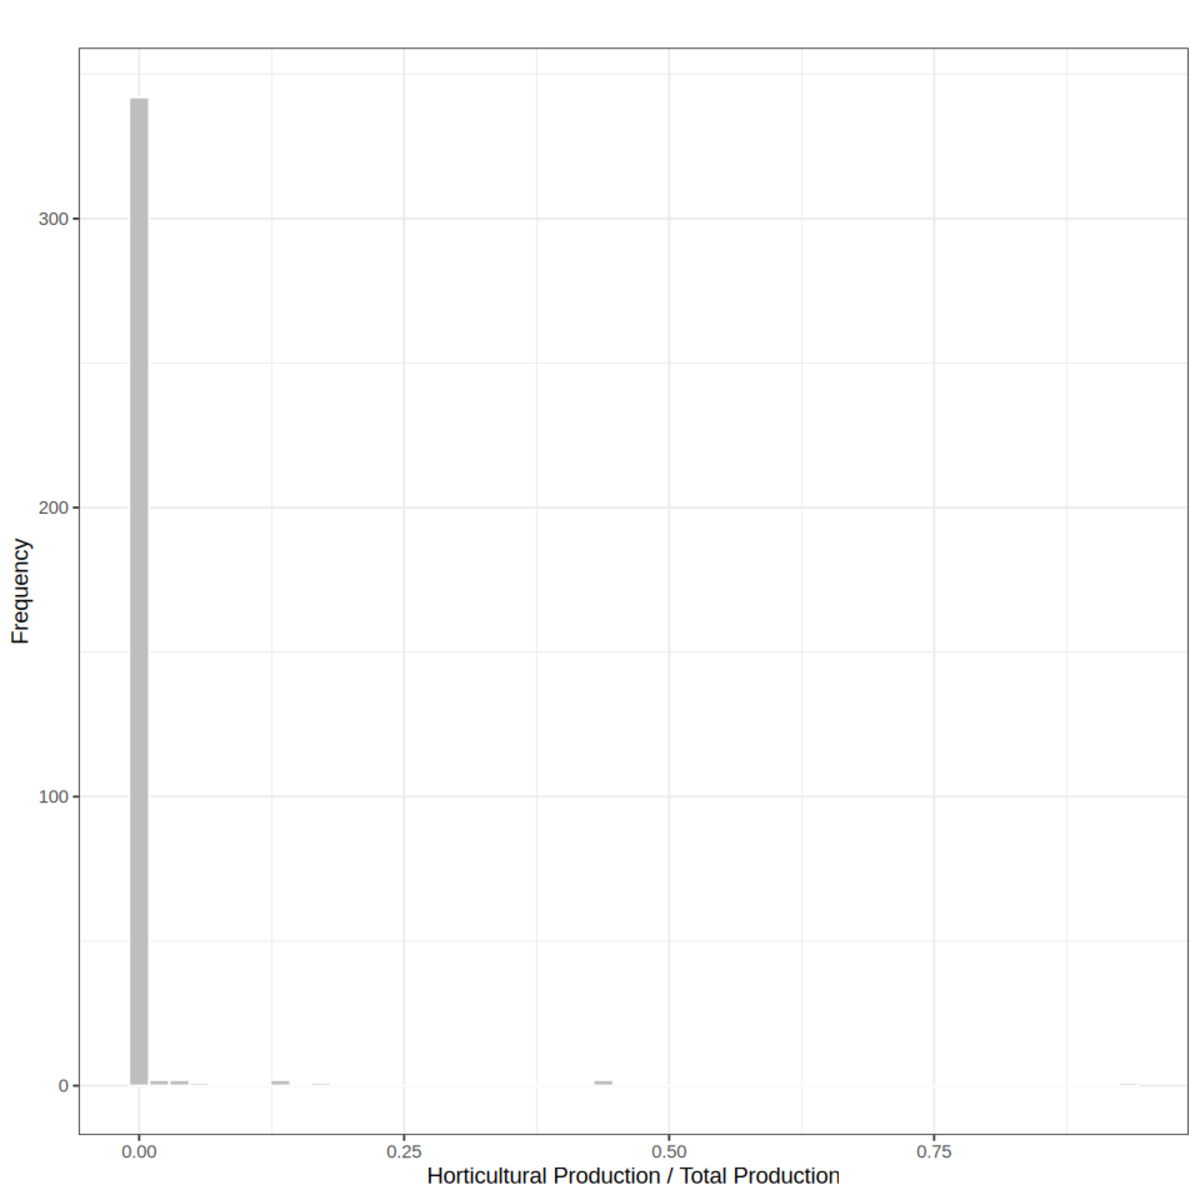
\includegraphics[
        width=0.8\textwidth,
        height=0.6\textheight
    ]{figures/hist_hort_tot.pdf}
    \caption{Distribution of the Share of Horticultural in Total Production}
    \label{fig:hist-hort-tot}
\end{figure}

% \begin{figure}[H]
%    \centering
%    \includegraphics[
%        width=0.8\textwidth,
%        height=0.6\textheight
%    ]{figures/%hist_log_yield_ha.pdf}
%    \caption{Distribution of Log revenue per Hectare.}
%    \label{fig:dist-yield-ha}
%\end{figure}

\begin{figure}[H]
    \centering
    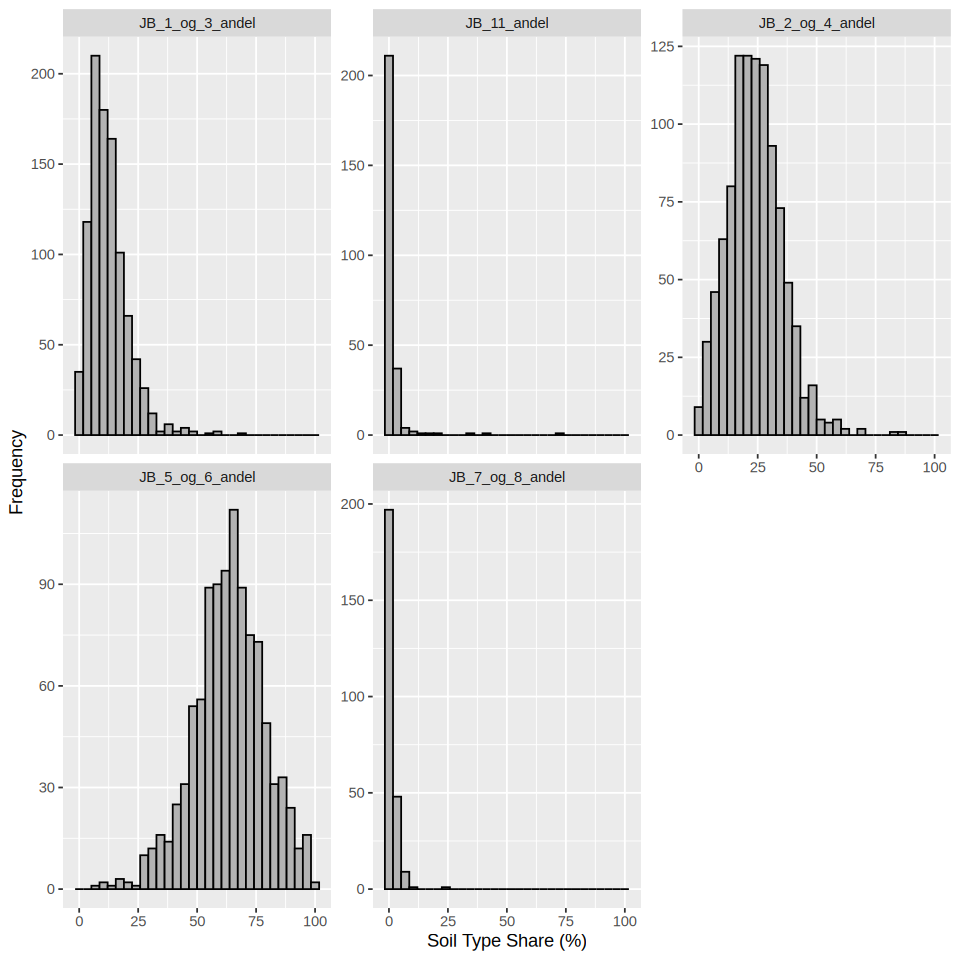
\includegraphics[
        width=1\textwidth,
        height=0.6\textheight
    ]{figures/hist_share_soil.png}
    \caption{Distribution of the Shares of Soil Types (\%) Used in the Empirical Analyses.}
    \label{fig:hist-share-soil}
\end{figure}


\newpage


\subsubsection*{Tables}

\begin{table}[htbp]
\centering
\small
\caption{Descriptive Statistics: Output Panel Data Set}
\label{tab:desc-stats-yield}
\begin{threeparttable}
\begin{tabular}{lrrrrr}
\toprule
 & \textbf{Mean} & \textbf{Median} & \textbf{St. Dev.} & \textbf{Min.} & \textbf{Max.} \\
\midrule
\addlinespace
\multicolumn{6}{l}{\textit{Dependent variable}} \\
\text{ Log revenue per hectare} & 8.95 & 9.09 & 0.90 & 3.16 & 12.34 \\
\addlinespace
\multicolumn{6}{l}{\textit{Soil type shares}} \\
\text{ Fine sand}  & 0.25 & 0.18 & 0.27 & 0.00 & 1.00 \\
\text{ Coarse sand} & 0.12 & 0.02 & 0.18 & 0.00 & 1.00 \\
\addlinespace
\multicolumn{6}{l}{\textit{Sub-category shares}} \\
\text{ Winter barley}        & 0.03 & 0.00 & 0.11 & 0.00 & 1.00 \\
\text{ Fava beans}           & 0.01 & 0.00 & 0.12 & 0.00 & 1.00 \\
\text{ Early/seed potatoes}  & 0.00 & 0.00 & 0.04 & 0.00 & 1.00 \\
\text{ Consumption potatoes} & 0.00 & 0.00 & 0.06 & 0.00 & 1.00 \\
\text{ Horticultural seeds}  & 0.00 & 0.00 & 0.05 & 0.00 & 1.00 \\
\text{ Spring wheat}         & 0.00 & 0.00 & 0.05 & 0.00 & 1.00 \\
\addlinespace
\bottomrule
\end{tabular}
\begin{tablenotes}
\footnotesize
\item \textit{Notes:} The dependent variable is the natural logarithm of revenue per hectare measured in DKK per hectare. 
Soil type shares and sub-category shares are measured as fractions of total crop area, with loamy soil as the excluded base soil type. 
The sample consists of 3,232 farm--crop category observations
across 894 farms.
\end{tablenotes}
\end{threeparttable}
\end{table}


\newpage


\section{Variable Construction}
\label{sec:variable-construction}
The following sections describe how gross margin, costs, revenues, and farm characteristics are constructed based on SEGES' farm accounting data, the Danish Agricultural Agency's spatial (GIS) data source, as well as their Fertiliser accounts. 
Note that numbers in parantheses indicate crop codes ('afgroedekoder') defined in the GIS data, and reference numbers defined in SEGES' farm accounts.

\subsection{Production Branches}
\label{sec:production-branches} 
In total, we construct 19 crop branches, 5 livestock branches, and 3 other income branches.
Crop production branches are aggregated at the farm level based on agricultural areas provided by the Danish Agricultural Agency's GIS system \citep{landbrugsstyrelsen2026b}, while livestock and other income branches are constructed based on the data from SEGES' farm accounts. 
We rely on the Danish Agricultural Agency's spatial (GIS) data on agricultural areas because it is more detailed than the areas reported in SEGES’ farm accounts.  

\subsubsection{Crop Branches}
The crop production branches are defined as:
\begin{itemize}
    \item[] \textbf{PG$_\textbf{1}:$ Spring barley (ha)} 
    \begin{itemize}
        \item[$+$] \textit{Vårbyg (1)}
    \end{itemize}
    \item[] \textbf{PG$_\textbf{2}:$ Winter barley (ha)}
    \begin{itemize}
        \item[$+$] \textit{Vinterbyg (10)}
    \end{itemize}
    \item[] \textbf{PG$_\textbf{3}:$ Winter wheat (ha)}
    \begin{itemize}
        \item[$+$] \textit{Vinterhvede (11)}
        \item[$+$] \textit{Vinterhvede, brødhvede (13)}
    \end{itemize}
    \item[] \textbf{PG$_\textbf{4}:$ Spring-sown cereals and mixed grains (ha)}
    \begin{itemize}
        \item[$+$] \textit{Vårhavre (3)}
        \item[$+$] \textit{Vårhvede (2)}
        \item[$+$] \textit{Vårhvede, brødhvede (6)}
        \item[$+$] \textit{Blanding af vårsåede arter (4)}
        \item[$+$] \textit{Vårtriticale (56)}
        \item[$+$] \textit{Vårrug (55)}
    \end{itemize}
    These crops are grouped together as a single production category because they share a similar cost and revenue structure. 
    While winter oat is included, it is a very small part of the data set and does not significantly affect the overall cost patterns.
    Spring-sown crops dominate this group and are an important determinant of input use, planting schedules, and yield characteristics.
    
    \item[] \textbf{PG$_\textbf{5}:$ Rye and Triticale (ha)}
    \begin{itemize}
        \item[$+$] \textit{Vinterhybridrug (15)}
        \item[$+$] \textit{Vinterrug (14)}
        \item[$+$] \textit{Vintertriticale (16)}
    \end{itemize}
    \item[] \textbf{PG$_\textbf{6}:$ Sugar beet (ha)}
    \begin{itemize}
        \item[$+$] \textit{Sukkerroer til fabrik (160)}
        \item[$+$] \textit{Fodersukkerroer (280)}
    \end{itemize}
    \item[] \textbf{PG$_\textbf{7}:$ Seeds (ha)}
    \begin{itemize}
        \item[$+$] \textit{Rajgræs, almindelig (101)}
        \item[$+$] \textit{Rajgræsfrø, alm. 1. år, efterårsudlagt (102)}
        \item[$+$] \textit{Timothefrø (105)}
        \item[$+$] \textit{Hundegræsfrø (106)}
        \item[$+$] \textit{Engsvingelfrø (107)}
        \item[$+$] \textit{Rødsvingelfrø (108)}
        \item[$+$] \textit{Rajsvingelfrø (109)}
        \item[$+$] \textit{Svingelfrø, strand- (111)}
        \item[$+$] \textit{Engrapgræsfrø (marktype) (112)}
        \item[$+$] \textit{Engrapsgræsfrø (plænetype) (113)}
        \item[$+$] \textit{Rajgræs, efterårsudl. hybrid (117)}
        \item[$+$] \textit{Kløverfrø (120)}
        \item[$+$] \textit{Spinatfrø (124)}
        \item[$+$] \textit{Dildfrø (651)}
        \item[$+$] \textit{Olieræddike til frø, radisefrø (655)}
        \item[$+$] \textit{Purløgsfrø (666)}
        \item[$+$] \textit{Blomsterfrø (668)}
    \end{itemize}
    \item[] \textbf{PG$_\textbf{8}:$ Potatoes (ha)}
    \begin{itemize}
        \item[$+$] \textit{Kartofler, lægge- (certificerede) (149)} 
        \item[$+$] \textit{Kartofler, lægge- (egen opformering) (150)}
        \item[$+$] \textit{Kartofler, stivelses- (151)}
        \item[$+$] \textit{Kartofler, spise- (pakkeri, vejsalg) (152)}
        \item[$+$] \textit{Kartofler, pulver/granules- (155)}
        \item[$+$] \textit{Kartofler, friteret/chips/pommes frites (156)}
        \item[$+$] \textit{Kartofler, spise- tidligt høstede med efterafgrøder (157)}
    \end{itemize}
    This category includes various types of potatoes, which have a distinct cost and production structure. 
    However, potatoes are not a focus crop in our data, and their limited representation means they are treated primarily for completeness rather than detailed analysis.
    
    \item[] \textbf{PG$_\textbf{9}:$ Rapeseed (ha)}
    \begin{itemize}
        \item[$+$] \textit{Vårraps (21)}
        \item[$+$] \textit{Vinterraps (22)}
    \end{itemize}
    \item[] \textbf{PG$_{\textbf{10}}:$ Legumes (ha)}
    \begin{itemize}
        \item[$+$] \textit{Korn og bælgsæd (over 50 \% bælgsæd) (18)}
        \item[$+$] \textit{Ærter (30)}
        \item[$+$] \textit{Hestebønner (31)}
        \item[$+$] \textit{Lupin (32)}
    \end{itemize}
    \item[] \textbf{PG$_{\textbf{11}}:$ Rotation grass (ha)}
    \begin{itemize}
        \item[$+$] \textit{Lucerne, slæt (171)}
        \item[$+$] \textit{Lucernegræs, over 25\% græs til slæt inkl. eget foder (172)}
        \item[$+$] \textit{Kløvergræs til fabrik (174)}
        \item[$+$] \textit{Græs med kløver/lucerne, under 50 \% bælgpl. (omdrift) efterårsudlagt i vinterkorn til grønkorn (236)}
        \item[$+$] \textit{Miljøgræs MVJ-tilsagn (0 N), omdrift (247)}
        \item[$+$] \textit{Græs med kløver/lucerne, under 50 \% bælgpl. (omdrift) (260)}
        \item[$+$] \textit{Kløvergræs, over 50\% kløver (omdrift) (261)}
        \item[$+$] \textit{Lucernegræs, over 50\% lucerne (omdrift) (262)}
        \item[$+$] \textit{Græs uden kløvergræs (omdrift) (263)}
        \item[$+$] \textit{Græs og kløvergræs uden norm, under 50 \% kløver (omdrift) (264)}
        \item[$+$] \textit{Græs under 50\% kløver/lucerne, ekstremt lavt udbytte (omdrift) (266)}
        \item[$+$] \textit{Græs  under 50\% kløver/lucerne, meget lavt udbytte (omdrift) (267)}
        \item[$+$] \textit{Græs under 50\% kløver/lucerne, lavt udbytte (omdrift) (268)}
        \item[$+$] \textit{Græs til udegrise, omdrift (270)}
        \item[$+$] \textit{Græs og kløvergræs uden norm, over 50 \% kløver (omdrift) (285)}
        \item[$+$] \textit{Markbræmme, på omdrift, slåning (327)}
        \item[$+$] \textit{Græs i omdrift, uden udbetaling af økologi-tilskud (306)}
    \end{itemize}
    \item[] \textbf{PG$_{\textbf{12}}:$ Whole crops without maize (ha)}
    \begin{itemize}
        \item[$+$] \textit{Vårbyg, helsæd (210)}
        \item[$+$] \textit{Vårhavre, helsæd (212)}
        \item[$+$] \textit{Blandkorn, vårsået, helsæd (213)}
        \item[$+$] \textit{Korn og bælgsæd, helsæd, under 50\% bælgsæd (214)}
        \item[$+$] \textit{Ærtehelsæd (215)}
        \item[$+$] \textit{Vinterhvede, helsæd (221)}
        \item[$+$] \textit{Vinterrug, helsæd (222)}
        \item[$+$] \textit{Blanding af vårkorn, grønkorn (230)}
        \item[$+$] \textit{Korn og bælgsæd, grønkorn, under 50\% bælgsæd (234)}
        \item[$+$] \textit{Grønkorn af vårbyg (701)}
        \item[$+$] \textit{Grønkorn af vårhvede (702)}
        \item[$+$] \textit{Grønkorn af vårhavre (703)}
        \item[$+$] \textit{Grønkorn af vårrug (704)} 
        \item[$+$] \textit{Grønkorn af vinterbyg (706)}
        \item[$+$] \textit{Grønkorn af vinterhvede (707)}
        \item[$+$] \textit{Grønkorn af vinterrug (709)}
    \end{itemize}
    This production branch includes cereals, legumes, and mixed crops harvested as whole crop or green forage, including both spring- and winter-sown varieties. 
    
    \item[] \textbf{PG$_{\textbf{13}}:$ Permanent grass (ha)}
    \begin{itemize}
        \item[$+$] \textit{Permanent græs, meget lavt udbytte (250)}
        \item[$+$] \textit{Permanent græs, lavt udbytte (251)}
        \item[$+$] \textit{Permanent græs, normalt udbytte (252)}
        \item[$+$] \textit{Miljøgræs MVJ-tilsagn (0 N), permanent (254)}
        \item[$+$] \textit{Permanent græs, under 50\% kløver/lucerne (255)}
        \item[$+$] \textit{Permanent kløvergræs, over 50\% kløver/lucerne (256)}
        \item[$+$] \textit{Permanent græs, uden kløver (257)}
        \item[$+$] \textit{Permanent græs og kløvergræs uden norm, under 50 \% kløver (276)}
        \item[$+$] \textit{Permanent græs og kløvergræs uden norm, over 50 \% kløver (286)}
        \item[$+$] \textit{Permanent græs, uden udbetaling af økologi-tilskud (305)}
    \end{itemize}
    \item[] \textbf{PG$_{\textbf{14}}:$ Maize for whole crops (ha)}
    \begin{itemize}
        \item[$+$] \textit{Silomajs (216)}
        \item[$+$] \textit{Silomajs med græsudlæg (218)}
    \end{itemize}
    \item[] \textbf{PG$_{\textbf{15}}:$ Energy crops (ha)}
    \begin{itemize}
        \item[$+$] \textit{Pil (592)}
        \item[$+$] \textit{Poppel (593)}
        \item[$+$] \textit{Lavskov (591)}
        \item[$+$] \textit{Elefantgræs (596)}
    \end{itemize}
    \item[] \textbf{PG$_{\textbf{16}}:$ Horticultural crops (ha)}
    \begin{itemize}
        \item[$+$] \textit{Jordskokker, konsum (429)}
        \item[$+$] \textit{Grøntsager, blandinger (450)}
        \item[$+$] \textit{Asparges (401)}
        \item[$+$] \textit{Jordbær (513)}
        \item[$+$] \textit{Sødkirsebær uden undervækst af græs (524)}
        \item[$+$] \textit{Æbler (528)}
        \item[$+$] \textit{Centnergræskar (553)}
        \item[$+$] \textit{Spinat (422)}
        \item[$+$] \textit{Blandet frugt (539)}
        \item[$+$] \textit{Vindrue (530)}
    \end{itemize}
    This production branch includes horticultural crops such as vegetables, fruits, and specialty crops. 
    These crops are grouped together because they are minor in area compared to the main cereals and forage crops.
    
    \item[] \textbf{PG$_{\textbf{17}}:$ Christmas trees (ha)}
    \begin{itemize}
        \item[$+$] \textit{Juletræer og pyntegrønt (583)}
    \end{itemize}
    \item[] \textbf{PG$_{\textbf{18}}:$ Fallow (ha)}
    \begin{itemize}
        \item[$+$] \textit{Brak, slåning (310)}
        \item[$+$] \textit{Bestøverbrak (342)}
        \item[$+$] \textit{Blomsterbrak (324)}
        \item[$+$] \textit{Brak langs vandløb og søer, slåning (alternativ til efterafgrøder) (345)}
    \end{itemize}
    \item[] \textbf{PG$_{\textbf{19}}:$ Other sales crops (ha)}
    \begin{itemize}
        \item[$+$] \textit{Vinterhavre (57)}
        \item[$+$] \textit{Korn og bælgsæd, under 50\% bælgsæd (7)}
        \item[$+$] \textit{Boghvede (53)}
        \item[$+$] \textit{Gul sennep (180)}
        \item[$+$] \textit{Solsikke (24)}
        \item[$+$] \textit{Majs til modenhed (5)}
        \item[$+$] \textit{Majs til modenhed med græsudlæg (19)}
    \end{itemize}
    This category collects crops that do not fit into the main production groups, including minor cereals, buckwheat, yellow mustard, sunflower, and maize for maturity. It is treated as a residual group, and while these crops are included for completeness, they are not a primary focus of the analysis.
\end{itemize}

\subsubsection{Excluded Areas}
\label{sec:excluded-areas}
The following land use categories are excluded from the empirical analysis, as they do not represent active crop or livestock production or are otherwise outside the focus of the data set.
See the Danish Agricultural Agency's website \citep{landbrugsstyrelsen2026e}, for more information on the crop categories, e.g., whether the crop area is in rotation and obliged to receive income support.
The excluded areas are:
\begin{itemize} 
    \item \textit{Naturarealer, økologisk jordbrug (907)}
    \item \textit{Minivådområder, projekttilsagn (322)}
    \item \textit{20-årig Udtagning med fastholdelse, ej landbrugsareal (316)}
    \item \textit{Ikke støtteberettiget landbrugsareal (361)}
    \item \textit{MVJ ej udtagning, ej landbrugsareal (318)}
    \item \textit{Miljøtiltag, ej landbrugsarealer (319)}
    \item \textit{Rekreative formål (271)}
    \item \textit{Intern kode: Bar jord (?)}
    \item \textit{Anden skovdrift (580)}
    \item \textit{Skovdrift med fjernelse af ved (581)}
    \item \textit{Skovlandbrug, ikke støtteberettiget (487)}
    \item \textit{Lysåbne arealer i skov (903)}
    \item \textit{Skovrejsning (privat) - forbedring af vandmiljø og grundvandsbeskyttelse (576)}
    \item \textit{Skovrejsning, direktivimplementerende uden tilsagn ved Landbrugsstyrelsen (565)}
    \item \textit{Skovrejsning  (privat) ? kulstofbinding og grundvandsbeskyttelse (575)}
    \item \textit{Klimaskovrejsning, national ordning ej Landbrugsstyrelsen (566)}
\end{itemize}

\subsubsection{Livestock Branches}
In addition to the crop production branches, we construct livestock branches in cases where farms have mixed crop/livestock production. 
We do not specify a branch for mink (\textit{Antal minktæver (5410)}) as all observations 'produce' zero mink. 
Moreover, we do not specify a branch for sheep (\textit{Antal moderfår (5450)}), since only two observations in the sample 'produce' sheep, and since these are mainly specialised in cattle production with relatively large areas of crop rotation grasses.
The livestock production branches are defined as:
\begin{itemize}
   \item[] \textbf{PG$_{\textbf{19m}}:$ Dairy cows (pcs)}
   \begin{itemize}
       \item[$+$] \textit{Årsskøer (5110)}
   \end{itemize}
   \item[] \textbf{PG$_{\textbf{19k}}:$ Cattle (pcs)}
    \begin{itemize}
        \item[$+$] \textit{Ammekøer (5112)}
        \item[$+$] \textit{Antal årsopdræt, slagtekvier (5129)}
        \item[$+$] \textit{Antal slagterkalve produceret (5150)}
    \end{itemize}
    \item[] \textbf{PG$_{\textbf{19s}}:$ Sows (pcs)}
    \begin{itemize}
        \item[$+$] \textit{Alle søer, inkl. gylte (5210)}
    \end{itemize}
    \item[] \textbf{PG$_{\textbf{19g}}:$ Piglets and slaughterpigs (100 pcs)}
    \begin{itemize}
        \item[$+$] \textit{Antal smågrise produceret (15-35 kg) (5220)}
        \item[$+$] \textit{Antal slagtersvin produceret (5250)}
    \end{itemize}
    \item[] \textbf{PG$_{\textbf{19f}}:$ Poultry (1,000 pcs)}
     \begin{itemize}
        \item[$+$] \textit{Antal årshøns (5310)}
        \item[$+$] \textit{Antal slagterkyllinger produceret (5320) divided by a factor}
    \end{itemize}
    The factor is derived from official livestock-unit standards \citep{husdyrgoedning-bilag12017}, where 1 DE corresponds to 167 laying hens and 3500 broilers. 
    This means that one laying hen is equivalent to 3500/167 = 20.96 broilers in standardized production intensity. 
    The factor is used to aggregate heterogeneous poultry categories into a comparable weighted output measure.
\end{itemize}

\subsubsection{Other Income Branches}
We construct other income branches as aggregate variables based only on income from other sources that are ’produced’ with one of the input variables (see~\ref{sec:cost-variables}). 
Specifically, other income branches are defined as:
\label{sec:other-income-sources}
\begin{itemize}
        \item \textbf{PG$_{\textbf{20}}:$ Income from agricultural contractors (10,000 kr)} 
        \begin{itemize}
            \item[$+$] \textit{Maskinstationindtægter (205)} \\[1ex]
            When a farm performs contractor work for others (e.g., harvesting, plowing on neighboring farms), it may use the farm’s own machinery, fuel, labor, and maintenance — all of which are included as inputs.
        \end{itemize}
        \item \textbf{PG$_{\textbf{21}}:$ Income from rental (e.g., of buildings) (10,000 kr)}
        \begin{itemize}
            \item[$+$] \textit{Lejeindtægter (7751)} \\[1ex]
            Energy is included as input, meaning a farm may bear some of the cost of maintaining and financing structures related to rented buildings. 
            If part of the building capacity is rented out to third parties, the income from that rental is an output of inputs already in the cost variables. 
        \end{itemize}
        \item \textbf{PG$_{\textbf{22}}:$ 
        Income from other sources (10,000 kr)}
        \begin{itemize}
            \item[$+$] \textit{Pasningsaftale (for mark og husdyr) (hhv. 7752, 7753, 7754, 7756)}
            \item[$+$] \textit{Vidersalg (7755)}
            \item[$+$] \textit{Vindmøller (7757)}
            \item[$+$] \textit{Skov (7759)}
            \item[$+$] \textit{Salg af sten, sand og grus (7761)}
        \end{itemize}
\end{itemize}

\subsection{Gross Margins}
\label{sec:gross-margin-ii}
In this thesis, we consistently use the following definition of Gross Margin II (DBII) based on the constructed costs and revenues (see Appedix~\ref{sec:cost-variables} and~\ref{sec:revenues}):
\begin{itemize}
    \item[] \textbf{$\mathrm{\textbf{DBII}^{\textbf{farmer}}}$ $\textbf{=}$}
    \begin{itemize}
        \item[$+$] Total crop revenues (kr)
        \item[$-$] Seed layout (kr)
        \item[$-$] Fertiliser (kr)
        \item[$-$] Plant protection (kr)
        \item[$-$] Miscellaneous regarding field use (kr)
        \item[$-$] Agricultural contractor service (kr)
        \item[$-$] Energy (kr)
        \item[$-$] Fuel (kr)
        \item[$-$] Labor (kr)
        \item[$-$] Maintenance, field implements (kr)
        \item[$-$] Depreciations, field implements (kr)
    \end{itemize}
\end{itemize}

\subsection{Costs}
\label{sec:cost-variables}
Cost variables is constructed from aggregate accounting items from SEGES' farm accounts.
The following lists describe each cost variable included in the analysis.

\subsubsection{Variable Costs} 
The variable costs form the basis for the analysis. 
In accordance with SEGES gross margin measure, we define the following variable costs directly related to crop production:
\begin{itemize}
    \item[] \textbf{OMK$_\textbf{1}:$ Seed layout (kr)}
    \begin{itemize}
        \item[$+$] \textit{Udsæd (230)}
    \end{itemize}
    Represents the seed costs attributable to the current planning period. 
    This includes both internally transferred seed and newly purchased seed.
    Potential issues: There may be variation in how internally produced seed is valued and recorded. 
    Seed costs are allocated to crop production branches, as every crop category requires seed inputs. 
    Seed costs are not allocated to livestock production branches, machinery income, rental income, other income, as these branches do not involve seed use.
    
    \item[] \textbf{OMK$_\textbf{2}:$ Fertiliser (kr)}   \begin{itemize}
        \item[$+$] \textit{Handelsgødning (235)}
    \end{itemize}
    Represents costs for various types of commercial fertilisers (nitrogen (N), phosphor (P), potassium (K) and combined products such as NPK, PK, and NK), as well as purchased manure.
    Fertiliser costs are allocated to all crop production branches, reflecting that nitrogen and other nutrients are applied across all crop types. 
    Fertiliser costs are not allocated to livestock production branches or other income branches.
    
    Potential issues: fertiliser prices can fluctuate substantially within and between planning periods, so differences in stock and timing of purchases may affect comparability between farms and fields. 
    Additionally, manure costs are likely to vary geographically depending on livestock intensity: some crop producers in livestock-dense areas may receive manure at no cost, while in other regions it represents an actual expense.

    \item[] \textbf{OMK$_\textbf{3}:$ Plant protection (kr)}
    \begin{itemize}
        \item[$+$] \textit{Planteværn (240)}
    \end{itemize}
    Represents costs for plant protection products such as pesticides, herbicides, and fungicides attributable to the planning period.
    Plant protection costs are allocated to all crop production branches. 
    Pesticide and herbicide use occurs across all crop types, though intensity varies. 
    Plant protection costs are not allocated to livestock or other income branches.

    \item[] \textbf{OMK$_\textbf{4}:$ Miscellaneous regarding field use (kr)}
    \begin{itemize}
        \item[$+$] \textit{Diverse vedrørende markbrug (245)}
    \end{itemize}
    Represents a broad category of miscellaneous costs related to field use within the planning period. 
    This includes, but is not limited to, transport and sales-related costs, drying and storage costs, sorting, plastic, and advisory services related to crop production.
    Miscellaneous field costs are allocated to all crop production branches. 
    They are not allocated to livestock or other income branches.
    The category is inherently heterogeneous, as it aggregates a wide range of unlike cost types. The degree of heterogeneity makes the category less comparable across farms and fields. 
    As such, it should be interpreted as a residual category rather than a fully standardized cost group.
\end{itemize} 

\subsubsection{Semi-Variable and Fixed Costs} 
Together with variable costs, semi-variable and fixed costs form the basis for Gross Margin II, providing a more complete picture of the costs attributable to each farm or field.
We define the semi-variable and fixed costs as:
\begin{itemize}
    \item[] \textbf{OMK$_\textbf{5}:$ Agricultural contractor services (kr)}
    \begin{itemize}
        \item[$+$] \textit{Høst af korn og frøafgrøder (310)}
        \item[$+$] \textit{Optagning (315)}
        \item[$+$] \textit{Høst af grovfoder (320)}
        \item[$+$] \textit{Udbringning af husdyrgødning (325)}
        \item[$+$] \textit{Maskinstation diverse (330)}
    \end{itemize}
    Represents costs for external machine services used in both crop/livestock production during the planning period. 
    This includes harvesting of cereals and seed crops (310), crop lifting (315), harvest of forage crops (320), spreading of manure (325), and the aggregated machine station category (330). 
    Agricultural contractor services are calculated as the sum of all above categories in accordance with SEGES' practice. 
    Costs associated with agricultural contractor services are allocated to all crop production branches as well as all livestock production branches, reflecting that machinery (services) is used across both crop and livestock operations.  
    They are not allocated to other income branches (machinery income, rental income, and other income), as these represent passive revenue streams rather than productive activities that directly consume external machinery services. 
    
    Potential issues: aggregation across sub-categories may mask systematic differences in reporting behavior, as some farms report detailed items while others rely on aggregated entries. This may introduce aggregation bias if the composition of services differs systematically across farms. Consequently, OMK$_5$ should be interpreted as a composite measure of external machinery use rather than a homogeneous cost input.
    
    \item[] \textbf{OMK$_\textbf{6}:$ Energy (kr)}
    \begin{itemize}
        \item[$+$] \textit{Energi excl. brændstof (300)}
    \end{itemize}
    Energy costs --- covering heating oil, solid fuel, gas, electricity, and electricity taxes --- are allocated to all crop production branches, all livestock production branches, machinery income, rental income, and other income, reflecting that energy consumption is pervasive across virtually all farm activities. 

    \item[] \textbf{OMK$_\textbf{7}:$ Fuel (kr)}
    \begin{itemize}
        \item[$+$] \textit{Brændstof (305)}
    \end{itemize}
    Represents costs for fuel used on the farm during the planning period. It includes fuel costs for vehicles and machinery, including diesel, petrol, and related taxes (305).
    Fuel costs are allocated to all production branches, reflecting that fuel is consumed in field operations, livestock management, and general farm machinery use. 
    Fuel costs are not allocated to rental income.
    Potential issues: Price fluctuations in fuel can affect costs for the planning period, for instance if purchases are made in advance.

    \item[] \textbf{OMK$_\textbf{8}:$ Labor (kr)}
       \begin{itemize}
        \item[$+$] \textit{Lønomkostninger (360)}
        \item[$+$] \textit{Ejerløn (heltid $\lor$ deltid)}
        \item[$-$] \textit{Personlig indtjening (7960)}
    \end{itemize}
    Labor costs are allocated to all production branches without exception, including all crop branches, all livestock branches, other income branches, reflecting that labor is a universal input across all farm activities.
    Labor costs consist of hired labor expenses and an imputed value of the owner’s labor. 
    The owner’s labor is classified based on norm hours, such that farms requiring at least 1,665 norm hours\footnote{Norm hours is the standardized calculated labor requirement of the farm over a year, which is based on the farm's size and production activities (e.g. crops and livestock), rather than actual recorded working hours.}, are classified as full-time, while farms below this threshold are classified as part-time. 
    For full-time farms, the owner’s labor is valued at 600,000 DKK annually, whereas for part-time farms it is set at 300,000 DKK. In both cases, the imputed labor value is adjusted for external income, reflecting that off-farm earnings reduce the required remuneration from the farm business. However, this adjustment is capped at 500,000 DKK for full-time farms and 200,000 DKK for part-time farms, thereby ensuring a minimum imputed owner labor value of 100,000 DKK.

   This approach deviates from the SEGES framework, where the farmer’s income is calculated as a residual based on norm hours (\textit{Personlig indtjening (7960)}). 
   Instead, by imposing a fixed salary, labor costs become exogenous to farm size, allowing differences in costs to reflect scale and efficiency rather than being absorbed through a norm-based labor adjustment.
   
   Potential issues: The arbitrary threshold between full-time and part-time means that farms with norm hours near the cutoff are treated very differently, even if their actual labor requirements are almost identical. 
   In addition, this approach breaks the direct link between labor input (norm hours) and remuneration, which may lead to inconsistencies if farms with very different labor requirements are assigned identical owner salaries. 
   In addition this approach excludes any spouse or family labor.
   
   \item[] \textbf{OMK$_\textbf{9}:$ Maintenance, field implements (kr)}
   \begin{itemize}
       \item[$+$] \textit{Vedligehold, markredskaber (345)}
   \end{itemize}
   Maintenance costs are included if they are directly related to crop production. 
   This covers maintenance of field machinery such as tractors, irrigation systems, and other tools used in the fields.
   Maintenance costs for field equipment are allocated to all crop production branches and to machinery income, and other income, as field equipment is used directly in crop production and machinery-related activities. They are not allocated to livestock branches or rental income.

    \item[] \textbf{OMK$_\textbf{10}$: Depreciations, field implements (kr)}
    \begin{itemize}
        \item[$+$] \textit{Afskrivninger, markredskaber (430)}
    \end{itemize}
    Depreciation costs are included for assets directly used in crop production. This covers depreciation of field machinery such as tractors and harvesters (430).
    Depreciation of field equipment is allocated to all crop production branches, machinery income, or other income, reflecting that field equipment depreciates through use in crop production and related activities. 
    Depreciation is not allocated to livestock branches or rental income.
\end{itemize}


% \subsubsection{General Fixed Costs} 
%The general fixed costs are indirectly linked to crop production. These usually involves other maintenance and depreciations on the farm such as land improvements, real estate, barn equipment, farm buildings and equipment, etc. If farms have livestock production or mixed crop-livestock production they should be included in the empirical analysis. However, within the scope of this thesis, we exclude them from empirical analysis:
%\begin{itemize}
%    \item[] \textbf{OMK$_{\textbf{11}}:$ Other Maintenance (kr)}
%    \begin{itemize}
%        \item[$+$] \textit{Vedligehold grundforbedringer (340)}
%        \item[$+$] \textit{Vedligehold fast ejendom (335)}
%        \item[$+$] \textit{Vedligehold staldinventar (350)}
%        \item[$+$] \textit{Vedligehold stamplanter (342)}
%        \item[$+$] \textit{Vedligehold, andet inventar (355)}
%    \end{itemize}
%    \item[] \textbf{OMK$_{\textbf{12}}:$ Other Depreciation (kr)}
%    \begin{itemize}
%        \item[$+$] \textit{Afskrivninger grundforbedringer (420)}
%        \item[$+$] \textit{Afskrivning driftsbygninger (410)}
%        \item[$+$] \textit{Afskrivning driftsmidler (460)}
%        \item[$+$] \textit{Afskrivning stamplanter (342)}
%        \item[$+$] \textit{Afskrivning beboelse landbrug (417)} 
%        \item[$+$] \textit{Afskrivning staldinventar (440)}
%    \end{itemize}
%\end{itemize} 

% \subsubsection{Fertiliser Inputs}
% The following fertiliser variables are retrieved and constructed based on the Danish fertiliser accounts.
% \begin{itemize}
%    \item[] \textbf{Q$_{\textbf{1}}:$ Total Nitrogen Applied (kg)}
%    \begin{itemize}
%        \item[$+$] \textit{Samlet forbrug af handelsgødning i kg kvælstof (F\_706\_1)}
%        \item[$+$] \textit{Udbragt Kg N i anden husdyrgødnig og anden organisk gødning (F\_716)}
%    \end{itemize}
%    \item[] \textbf{Q$_{\textbf{2}}:$ Total corrected N quota (kg)}
%    \begin{itemize}
%        \item \textit{Bedriftens korrigerede N-kvote i alt (F\_512)}
%    \end{itemize}
% \end{itemize}

\subsection{Revenues}
\label{sec:revenues}
The crop revenues are constructed based on aggregate production values. 
Numbers in parentheses are the corresponding reference numbers reported in SEGES' farm accounts:
\begin{itemize}
    \item[] \textbf{U$_\textbf{1}:$ Barley (kr)}
    \begin{itemize}
        \item[$+$] \textit{Byg beholdning, ultimo (7055)}
        \item[$+$] \textit{Byg, kasseomsætning (salg) (7016)}
        \item[$+$] \textit{Byg, intern omsætning (7025)}
        \item[$-$] \textit{Byg beholdning, primo (7051)}
    \end{itemize}
    \item[] \textbf{U$_\textbf{2}:$ Wheat (kr)}
    \begin{itemize}
        \item[$+$] \textit{Hvede beholdning, ultimo (7063)}
        \item[$+$] \textit{Hvede, kasseomsætning (7020)}
        \item[$+$] \textit{Hvede, intern omæstning (7029)}
        \item[$-$] \textit{Hvede beholdning, primo (7059)}
    \end{itemize}
    \item[]  \textbf{U$_\textbf{3}:$ Oats \& Mixed grain (kr)}
    \begin{itemize}
        \item[$+$] \textit{Havre, ultimo (7077)}
        \item[$+$] \textit{Havre, kasseomsætning (7008)}
        \item[$+$] \textit{Havre, intern omsætning (7036)}
        \item[$-$] \textit{Havre, primo (7075)}
        \item[$+$] \textit{Øvrige korn, ultimo (7071)}
        \item[$+$] \textit{Øvrige korn, intern omæstning (7033)}
        \item[$-$] \textit{Øvrige korn, primo (7069)}
    \end{itemize}
    \item[] \textbf{U$_\textbf{4}:$ Rye \& Triticale (kr)}
    \begin{itemize}
        \item[$+$] \textit{Rug, ultimo (7082)}
        \item[$+$] \textit{Rug, kasseomsætning (7090)}
        \item[$+$] \textit{Rug, intern omsætning} (7045)
        \item[$-$] \textit{Rug, primo (7080)} 
        \item[$+$] \textit{Triticale, ultimo (7097)}
        \item[$+$] \textit{Triticale, kasseomsætning (7010)}
        \item[$+$] \textit{Triticale, intern omsætning (7038)}
        \item[$-$] \textit{Triticale, primo (7095)}
    \end{itemize}
    \item[] \textbf{U$_\textbf{5}:$ Sugar beet (kr)}
    \begin{itemize}
        \item[$+$] \textit{Sukkerroer (110)}
        \item[$+$] \textit{Fodersukkerroer (7214)}
    \end{itemize}
    \item[] \textbf{U$_\textbf{6}:$ Seeds (kr)}
    \begin{itemize}
        \item[$+$] \textit{Frø (105)}
    \end{itemize}
    \item[] \textbf{U$_\textbf{7}:$ Potatoes (kr)}
    \begin{itemize}
        \item[$+$] \textit{Kartofler (115)}
    \end{itemize}
    \item[] \textbf{U$_\textbf{8}:$ Rapeseed (kr)}
    \begin{itemize}
        \item[$+$] \textit{Raps (120)}
    \end{itemize}
    \item[] \textbf{U$_\textbf{9}:$ Legumes (kr)}
    \begin{itemize}
        \item[$+$] \textit{Ærter mv (125)}
    \end{itemize}
    \item[] \textbf{U$_{\textbf{10}}:$ Roughage w/o maize (kr)}
    \begin{itemize}
        \item[$+$] \textit{Sædskiftegræs (7216)}
        \item[$+$] \textit{Helsæd (7218)}
        \item[$+$] \textit{Vedvarende græs (7219)}
    \end{itemize}
     \item[] \textbf{U$_{\textbf{11}}:$ Maize for feed (kr)}
    \begin{itemize}
        \item[$+$] \textit{Majs til helsæd (7220)} 
        \item[$+$] \textit{Kolbemajs (7221)}
    \end{itemize}
    \item[] \textbf{U$_{\textbf{12}}:$ Energy crops (kr)}
    \begin{itemize}
        \item[$+$] \textit{Energiafgrøder (145)}
    \end{itemize}
    \item[] \textbf{U$_{\textbf{13}}:$ Horticultural crops (kr)}
    \begin{itemize}
        \item[$+$] \textit{Gartneriafgrøder (135)}
    \end{itemize}
    \item[] \textbf{U$_{\textbf{14}}:$ Other industrial crops (kr)}
    \begin{itemize}
        \item[$+$] \textit{Andre industriafgrøder (130)}
    \end{itemize}
    \item[] \textbf{U$_{\textbf{15}}:$ Perennial crops (kr)}
    \begin{itemize}
        \item[$+$] \textit{Andre landbrugsindtægter - del 2 (212)}
    \end{itemize}
\end{itemize}

\subsubsection{Mapping of Revenues}
\label{sec:mapping-yields-crops}
Table~\ref{tab:mapping-yields-crops} gives a best effort mapping of which crop categories created from the GIS areas that are used to generate which revenues in SEGES' farm accounts.

\begingroup
\fontsize{8.5}{10}\selectfont
\renewcommand{\arraystretch}{1.5}
\begin{longtable}{l | p{9cm}}
\caption{Mapping of revenue Categories.}
\label{tab:mapping-yields-crops} \\
\toprule
\textbf{SEGES -- Crop Revenues} & \textbf{GIS -- Crop Categories} \\
\midrule
\endfirsthead

 
\bottomrule
\endfoot
 
$U_1:$ Barley
       & \textit{Vårbyg} (1) \\
       & \textit{Vinterbyg} (10) \\ \midrule
 
$U_2:$ Wheat
       & \textit{Vinterhvede} (11) \\
       & \textit{Vinterhvede, brødhvede} (13) \\
       & \textit{Vårhvede} (2) \\
       & \textit{Vårhvede, brødhvede} (6) \\ \midrule
 
$U_3:$ Oats \& Mixed grain
       & \textit{Vårhavre} (3) \\
       & \textit{Vinterhavre} (57) \\
       & \textit{Blanding af vårsåede arter} (4) \\ \midrule
 
$U_4:$ Rye \& Triticale
       & \textit{Vinterrug} (14) \\
       & \textit{Vinterhybridrug} (15) \\
       & \textit{Vårrug} (55) \\
       & \textit{Vintertriticale} (16) \\
       & \textit{Vårtriticale} (56) \\ \midrule
 
$U_5:$ Sugar beet
       & \textit{Sukkerroer til fabrik} (160) \\
       & \textit{Fodersukkerroer} (280) \\ \midrule
 
$U_6:$ Seeds
       & \textit{Rajgræs, almindelig} (101) \\
       & \textit{Rajgræsfrø, alm. 1. år, efterårsudlagt} (102) \\
       & \textit{Timothefrø} (105) \\
       & \textit{Hundegræsfrø} (106) \\
       & \textit{Engsvingelfrø} (107) \\
       & \textit{Rødsvingelfrø} (108) \\
       & \textit{Rajsvingelfrø} (109) \\
       & \textit{Svingelfrø, strand-} (111) \\
       & \textit{Engrapgræsfrø (marktype)} (112) \\
       & \textit{Engrapsgræsfrø (plænetype)} (113) \\
       & \textit{Rajgræs, efterårsudl. hybrid} (117) \\
       & \textit{Kløverfrø} (120) \\
       & \textit{Spinatfrø} (124) \\
       & \textit{Dildfrø} (651) \\
       & \textit{Olieræddike til frø, radisefrø} (655) \\
       & \textit{Purløgsfrø} (666) \\
       & \textit{Blomsterfrø} (668) \\ \midrule
 
$U_7:$ Potatoes
       & \textit{Kartofler, lægge- (certificerede)} (149) \\
       & \textit{Kartofler, lægge- (egen opformering)} (150) \\
       & \textit{Kartofler, stivelses-} (151) \\
       & \textit{Kartofler, spise- (pakkeri, vejsalg)} (152) \\
       & \textit{Kartofler, pulver/granules-} (155) \\
       & \textit{Kartofler, friteret/chips/pommes frites} (156) \\
       & \textit{Kartofler, spise- tidligt høstede med efterafgrøder} (157) \\ \midrule
 
$U_8:$ Rapeseed
       & \textit{Vårraps} (21) \\
       & \textit{Vinterraps} (22) \\ \midrule
 
$U_9:$ Legumes
       & \textit{Ærter} (30) \\
       & \textit{Hestebønner} (31) \\
       & \textit{Lupin} (32) \\ \midrule
 
$U_{10}:$ Roughage w/o maize
       & \textit{Lucerne, slæt} (171) \\
       & \textit{Lucernegræs, over 25\% græs til slæt inkl. eget foder} (172) \\
       & \textit{Kløvergræs til fabrik} (174) \\
       & \textit{Græs med kløver/lucerne, under 50\% bælgpl. (omdrift) efterårsudlagt i vinterkorn til grønkorn} (236) \\
       & \textit{Miljøgræs MVJ-tilsagn (0 N), omdrift} (247) \\
       & \textit{Græs med kløver/lucerne, under 50\% bælgpl. (omdrift)} (260) \\
       & \textit{Kløvergræs, over 50\% kløver (omdrift)} (261) \\
       & \textit{Lucernegræs, over 50\% lucerne (omdrift)} (262) \\
       & \textit{Græs uden kløvergræs (omdrift)} (263) \\
       & \textit{Græs og kløvergræs uden norm, under 50\% kløver (omdrift)} (264) \\
       & \textit{Græs under 50\% kløver/lucerne, ekstremt lavt udbytte (omdrift)} (266) \\
       & \textit{Græs under 50\% kløver/lucerne, meget lavt udbytte (omdrift)} (267) \\
       & \textit{Græs under 50\% kløver/lucerne, lavt udbytte (omdrift)} (268) \\
       & \textit{Græs til udegrise, omdrift} (270) \\
       & \textit{Græs og kløvergræs uden norm, over 50\% kløver (omdrift)} (285) \\
       & \textit{Græs i omdrift, uden udbetaling af økologi-tilskud} (306) \\
       & \textit{Markbræmme, på omdrift, slåning} (327) \\

       & \textit{Vårbyg, helsæd} (210) \\
       & \textit{Vårhavre, helsæd} (212) \\
       & \textit{Blandkorn, vårsået, helsæd} (213) \\
       & \textit{Korn og bælgsæd, helsæd, under 50\% bælgsæd} (214) \\
       & \textit{Ærtehelsæd} (215) \\
       & \textit{Vinterhvede, helsæd} (221) \\
       & \textit{Vinterrug, helsæd} (222) \\
       & \textit{Blanding af vårkorn, grønkorn} (230) \\
       & \textit{Korn og bælgsæd, grønkorn, under 50\% bælgsæd} (234) \\
       & \textit{Grønkorn af vårbyg} (701) \\
       & \textit{Grønkorn af vårhvede} (702) \\
       & \textit{Grønkorn af vårhavre} (703) \\
       & \textit{Grønkorn af vårrug} (704) \\
       & \textit{Grønkorn af vinterbyg} (706) \\
       & \textit{Grønkorn af vinterhvede} (707) \\
       & \textit{Grønkorn af vinterrug} (709) \\

       & \textit{Permanent græs, meget lavt udbytte} (250) \\
       & \textit{Permanent græs, lavt udbytte} (251) \\
       & \textit{Permanent græs, normalt udbytte} (252) \\
       & \textit{Miljøgræs MVJ-tilsagn (0 N), permanent} (254) \\
       & \textit{Permanent græs, under 50\% kløver/lucerne} (255) \\
       & \textit{Permanent kløvergræs, over 50\% kløver/lucerne} (256) \\
       & \textit{Permanent græs, uden kløver} (257) \\
       & \textit{Permanent græs og kløvergræs uden norm, under 50\% kløver} (276) \\
       & \textit{Permanent græs og kløvergræs uden norm, over 50\% kløver} (286) \\
       & \textit{Permanent græs, uden udbetaling af økologi-tilskud} (305) \\ \midrule
 
$U_{11}:$ Maize for feed
       & \textit{Silomajs} (216) \\
       & \textit{Silomajs med græsudlæg} (218) \\ \midrule
 
$U_{12}:$ Energy crops
       & \textit{Lavskov} (591) \\
       & \textit{Pil} (592) \\
       & \textit{Poppel} (593) \\
       & \textit{Elefantgræs} (596) \\ \midrule
 
$U_{13}:$ Horticultural crops
       & \textit{Asparges} (401) \\
       & \textit{Spinat} (422) \\
       & \textit{Jordskokker, konsum} (429) \\
       & \textit{Grøntsager, blandinger} (450) \\
       & \textit{Jordbær} (513) \\
       & \textit{Sødkirsebær uden undervækst af græs} (524) \\
       & \textit{Æbler} (528) \\
       & \textit{Vindrue} (530) \\
       & \textit{Blandet frugt} (539) \\
       & \textit{Centnergræskar} (553) \\ \midrule
 
$U_{14}:$ Other industrial crops
       & \textit{Majs til modenhed} (5) \\
       & \textit{Majs til modenhed med græsudlæg} (19) \\
       & \textit{Boghvede} (53) \\
       & \textit{Korn og bælgsæd, under 50\% bælgsæd} (7) \\
       & \textit{Gul sennep} (180) \\
       & \textit{Solsikke} (24) \\ \midrule
 
$U_{15}:$ Perennial crops
       & \textit{Juletræer og pyntegrønt} (583) \\
 
\end{longtable}
\endgroup


\newpage


\subsection{Farm Characteristics and Dummy Variable}
\label{sec:farm-charactistics-organic-dummy}
\begin{itemize}
    \item[] \textbf{Z$_\textbf{1}:$ Livestock manure (kg nitrogen per ha)} \\[0.25cm]
    We obtain organic manure from the 'gødningsregnskaber', and include this variable as a Z variable rather than as a cost variable, since acquisition costs of organic manure is negligible. 
    However, there are still costs associated (e.g., field application), which seem reasonable to depend of the amount of manure spread out on the fields.
    \item[] \textbf{Z$_\textbf{2}:$ Areas that can be irrigated (ha)} \\[0.25cm]
    We include \textit{Arealer, der kan vandes (3946)}  to account for differences in production conditions across farms that are not captured by total farm size alone. For example, access to irrigation might increase yield potential and reduce dependency on weather conditions.
    \item[] \textbf{Z$_\textbf{3}:$ Farm size (ha)} \\[0.25cm]
    We account for economies of scale by including the size of the farm, which is calculated by the sum of all agricultural areas, i.e., the sum of all crop production branches: farm size = PG$_1 + \ldots + $ PG$_{19}$.
    % \item[] Z\_10: Livestock units per hectare, LU/ha (?)
    %\begin{itemize}
    \item[] \textbf{Z$_4$, Z$_5$, Z$_6$, Z$_7:$ Soil type shares (\%)} \\[0.25cm]
    We include farm-level shares of the following aggregated soil types: \textit{JB 1 og 3 grovsand}, \textit{JB 7 og 8 lerjord}, \textit{JB 5 og 6 lerjord}, \textit{JB 2 og 4 finsand}, and \textit{JB 11 humus}.
    The farm-level areas of each soil type are obtained by merging Landbrugsstyrelsens GIS data on field-level crops with their GIS data on soil qualities, and then aggregating to farm-level data. 
    To avoid multicollinearity in the empirical analysis, we exclude the share of loamy soil (\textit{JB 5 and 6 lerjord}), treating this soil type as our base type.
    For information on the soil types see the Ministry of Agriculture, Food and Fisheries's legal soil type classification \citep{jordbundstyper2024}. 
    \item[] \textbf{Z$_8$, Z$_9$, Z$_{10}:$ Livestock units (LU)} \\[0.25cm]
    We include livestock units for \textit{Antal DE Kvæg (5114)}, \textit{Antal DE Svin (5212)}, and \textit{Antal DE Fjerkræ (5304)} to allow for a meaningsful comparison of farms with different livestock-mixes.
    \item[] \textbf{Z$_{11}$, $\ldots$ , Z$_{25}$: Crop revenues (kr)}\\[0.25cm]
    The revenues for each crop category $\text{U}_1, \ldots, \text{U}_{15}$ are included as factors that can affect the input-output coefficients. The motivation is that input use and revenues are expected to be positively correlated: production branches with higher revenues typically require more inputs per hectare, such as more fertiliser, more plant protection, and more labor, in order to achieve those revenues. Conversely, production branches with lower revenues may reflect less intensive management and correspondingly lower input use. 
    By including revenues as allocation factors, the model allows input-output coefficients to vary  with the revenue-generating capacity of each crop category, rather than assuming uniform input intensity across all branches.
    \item[] \textbf{D$_\textbf{1}:$ Organic Dummy Variable} \\[0.25cm]
    Based on the variable \textit{Økologisk landbrug (6410)} from SEGES farm accounts, we construct a dummy variable equal to 1 if the farm is organic, and 0 if the farm is conventional.
\end{itemize}


\newpage


\section{Methodology}

\subsection{Estimating Nitrogen Damage Costs}

\subsubsection{Price Deflation and Currency Conversion}
\label{app:price-deflation}

The location-specific damage cost estimates from \citet{andersen2019} are 
reported in euros at 2016 prices. The uniform damage cost estimates from 
\citet{brink2011} are reported in euros at 2005 prices. Both sets of 
estimates are converted to Danish kroner at 2024 prices using two steps.

\paragraph {Currency conversion.} Damage cost estimates are converted to 
DKK using the average EUR/DKK exchange rate for 2024 of 7.4589, sourced from Eurostat \citep{Eurostat2024}.

\paragraph{Price deflation.} The resulting DKK values are adjusted to 2024 prices using the Danish Harmonised Index of Consumer Prices (HICP), sourced from Statistics Denmark \citep{DST2024HICP}. The deflation factor is 
calculated as the ratio of the average HICP in 2024 (98.191) to the average HICP in the base year of each estimate --- 2016 (82.494) for the location-specific estimates and 2005 (70.016) for the ENA estimates. This yields deflation factors of $98.191/82.494 = 1.1902$ and 
$98.191/70.016 = 1.4024$ respectively.

\begin{table}[H]
\label{fig:DC_calc}
\centering
\small
\begin{tabularx}{\textwidth}{r l l r r r r r r}
\toprule
ID15 & DC 2016 (EUR) & DKK & DC\_2024 & ENA\_low\_2024 & ENA\_up\_2024 & ENA\_mean\ 2024 \\
\midrule
131 &  1.35 & 10.070 & 11.986 & 52.302 & 209.209 & 130.755 \\
136 & 2.47 & 18.423 & 21.929 & 52.302 & 209.209 & 130.755 \\
165 & 7.81 & 58.254 & 69.339 & 52.302 & 209.209 & 130.755 \\
93  &  4.96 & 36.996 & 44.036 & 52.302 & 209.209 & 130.755 \\
128 & 9.89 & 73.769 & 87.805 & 52.302 & 209.209 & 130.755 \\
2   &  8.38 & 62.506 & 74.399 & 52.302 & 209.209 & 130.755 \\
\bottomrule
\end{tabularx}
\caption{Overview of coastal catchments and damage cost estimates}
\end{table}


\subsection{Estimating Field-Level Outputs (w. interaction terms)}
This model specification includes interaction terms and farm fixed effects.
Let $i = 1, \ldots, N$ index farm observations, $k = 1, \ldots, K$ crop categories with $K$ as the 'base' crop, and let $l = 1, \ldots, L$ crop sub-categories, and $f = 1, \ldots, F_{ik}$ fields that farm $i$ cultivates with crop category $k$.
Furthermore, let $s(i,k,f) \in \{1 = \text{fine sand}, 2 = \text{coarse sand}, 3 = \text{loamy soil}\}$ denote farm $i$'s predominant soil type on field $f$ with crop $k$. 
The specification of the model that we estimate (with three soil types) is:
\begin{equation}
\begin{aligned}
    \ln(y_{ik}/A_{ik}) = & \sum_{k'=1}^{K-1} \alpha_{k'} \mathbf{1}(k'=k) \\
    &+ \mu_1\,\text{fineshare}_{ik} 
    + \sum_{k'=1}^{K-1} \delta_{1k'}\,\text{fineshare}_{ik}\,\mathbf{1}(k'=k) \\
    &+ \mu_2\,\text{coarseshare}_{ik} 
    + \sum_{k'=1}^{K-1} \delta_{2k'}\,\text{coarseshare}_{ik}\,\mathbf{1}(k'=k) \\
    &+ \sum_{l=1}^{L} \rho_l\,\text{cropshare}_{il}\,D_{lk} 
    + \sum_{i'=1}^{N-1} \lambda_{i'} \mathbf{1}(i' = i) + \varepsilon_{ik},
    \end{aligned}
\end{equation}
\paragraph{Dependent variable.} The dependent variable, $\ln(y_{ik}/A_{ik})$, is the natural logarithm of farm $i$'s observed revenue per hectare from crop category $k$, where $y_{ik}$ is total output and $A_{ik}$ is total cultivated area.
The log transformation is appropriate for two reasons: it provides an economically meaningful scale for comparing revenues across farms with different geographic conditions, and it ensures that predicted values are always positive.


\paragraph{Explanatory variables.}
The first line contains crop indicator variables $\mathbf{1}(k'=k)$,
which equals one if the observation belongs to crop category $k'$ and
zero otherwise, capturing crop-specific revenue levels relative to the
base crop $K$.

The second and third lines contain the soil share variables. For example, fine sand share is defined as $\text{fineshare}_{ik} = \sum_f A_{ikf}\,\mathbf{1}(s=1) / A_{ik}$,
where $A_{ikf}$ is the area of field $f$ under crop category $k$ on
farm $i$. 
Coarse sand share, is defined analogously, while loamy soil is the excluded base soil type to avoid perfect multicollinearity.
Both soil shares enter as main effects and interacted with the
crop indicators, allowing the associated effect of soil type to
differ across crop categories.

The fourth line contains two additional variables.
The crop sub-category share, $\text{cropshare}_{il}$, captures the
within-category composition of crop sub-categories --- for example,
the share of winter barley within the barley category, defined as
$A_{i,\text{winterbarley}} / A_{i,\text{barley}}$.
The indicator $D_{lk}$ equals one if sub-category $l$ belongs to main
category $k$ and zero otherwise, ensuring that each sub-category share
only enters for its relevant main crop category.
Farm fixed effect indicators $\mathbf{1}(i'=i)$ equal one for farm
$i'$ and zero otherwise, with one farm serving as the base to avoid
perfect multicollinearity.

\paragraph{Parameters.}
The parameter $\alpha_{k'}$ measures the log revenue differential for crop category $k'$ relative to the base crop category $K$.
The parameters $\mu_1$ and $\mu_2$ measure the association between the fine sand and coarse sand shares and log revenue per hectare for the base crop category, relative to loamy soil.
The differential parameters $\delta_{1k'}$ and $\delta_{2k'}$ capture how these soil effects vary across crop categories relative to the base crop $K$, reflecting that the revenue reduction associated with sandy soils may differ between, for instance, barley and rapeseed.
The coefficient $\rho_l$ measures the revenue differential of sub-category $l$ relative to the within-category base sub-category --- for instance, $\rho_{\text{winterbarley}} > 0$ indicates that winter barley revenues are higher per hectare than spring barley within the barley category.
The farm fixed effects $\lambda_{i'}$ absorb unobserved heterogeneity at the farm level.
Finally, $\varepsilon_{ik}$ is the error term.

\subsubsection{Field-level Allocation}
Based on the estimated coefficients from equation~(\ref{eq:est-model-spec-estimated}), we define predicted relative revenues for each soil type and crop category combination.
These predicted relative revenues for the base crop category $K$ are defined as:
\begin{align*}
    \nu_{i1Kl} & = \exp\!\left(\lambda_i + \mu_1 + \sum_{l=1}^{L} \rho_l\,\text{cropshare}_{il}\,D_{lK}\right), \\
    \nu_{i2Kl} & = \exp\!\left(\lambda_i + \mu_2 + \sum_{l=1}^{L} \rho_l\,\text{cropshare}_{il}\,D_{lK}\right), \\
    \nu_{i3Kl} & = \exp\!\left( \lambda_i + \sum_{l=1}^{L} \rho_l\,\text{cropshare}_{il}\,D_{lK} \right),
\end{align*}
while for any other crop category $k \neq K$ they are defined as:
\begin{align*}
    \nu_{i1kl} & = \exp\!\left(\lambda_i + \alpha_k + \mu_1 + \delta_{1k} + \sum_{l=1}^{L} \rho_l\,\text{cropshare}_{il}\,D_{lk}\right), \\
    \nu_{i2kl} & = \exp\!\left(\lambda_i + \alpha_k + \mu_2 + \delta_{2k} + \sum_{l=1}^{L} \rho_l\,\text{cropshare}_{il}\,D_{lk}\right), \\
    \nu_{i3kl} & = \exp\!\left(\lambda_i + \alpha_k + \sum_{l=1}^{L} \rho_l\,\text{cropshare}_{il}\,D_{lk}\right).
\end{align*}
Thus, $\nu_{sK}$ and $\nu_{sk}$ gives the predicted revenue per hectare associated with soil type $s$ and crop category $k$, incorporating both soil type effects and crop sub-category composition.
For example, values $\nu_{1K}$ > 1 indicate higher revenue per hectare on fine sand, relative to the base crop category $K$ on loamy soil, while values $\nu_{1K}$ < 1 indicate lower revenue per hectare on fine sand, relative to the base crop category $K$ on loamy soil.

Farm $i$'s observed output from crop category $k$ is then allocated to fields proportionally with both field size and predicted relative revenues:
\begin{align}
    \hat{y}_{ikf} = y_{ik} \cdot \frac{A_{ikf} \cdot \nu_{s(i,k,f),kl}}
    {\sum_{f'=1}^{F_{ik}} A_{ikf'} \cdot \nu_{s(i,k,f'),kl}}
\end{align}
where $A_{ikf}$ is farm $i$'s observed area on field $f$ for crop category $k$.
By construction, $\sum_{f=1}^{F_{ik}} \hat{y}_{ikf} = y_{ik}$, ensuring that field-level allocations sum to the observed farm-level totals.


\subsection{Estimating Field-Level Inputs}
\label{sec:input-model}
This model specification includes farm fixed effects.
Let $i = 1, \ldots, N$ index farm observations, $j = 1, \ldots, J$ index production branches with $J$ as the base branch, $f = 1, \ldots, F_{ij}$ fields that farm $i$ cultivates with production branch $j$, and $p = 1, \ldots, P$ index the type of input or cost variable being estimated. Furthermore, let $s(i,j,f) \in \{1 = \text{fine sand}, 2 = \text{coarse sand}, 3 = \text{loamy soil}\}$ denote farm $i$'s predominant soil type on field $f$ with production branch $j$.

The model is estimated separately for each input $p$.
The specification of the model that we estimate (with three soil types) is:
\begin{equation}
\begin{aligned}
    \ln(\hat{x}_{ij}^p / A_{ij}) = & \sum_{j'=1}^{J-1} \alpha_{j'}^p \mathbf{1}(j'=j) \\
    &+ \mu_1^p\,\text{fineshare}_{ij}
    + \mu_2^p\,\text{coarseshare}_{ij} \\
    &+ \lambda_i^p + \varepsilon_{ij}^p,
    \label{eq:model-spec-inputs}
\end{aligned}
\end{equation}
with:
\begin{itemize}
    \item $\hat{x}_{ij}^p =$ farm $i$'s estimated quantity of input $p$ used in production branch $j$.
    \item $A_{ij} =$ farm $i$'s observed area of production branch $j$.
    \item $\hat{x}_{ij}^p / A_{ij} =$ farm $i$'s estimated input $p$ use per hectare in production branch $j$.
    \item $\text{fineshare}_{ij}$, $\text{coarseshare}_{ij} =$ farm $i$'s observed shares of fine sandy and coarse sandy soils in production branch $j$, e.g., $\text{fineshare}_{ij} = \sum_f A_{ijf} \mathbf{1}(s = 1) / A_{ij}$, where $A_{ijf}$ is farm $i$'s observed area of production branch $j$ on field $f$. Loamy soil is the excluded base soil type to avoid perfect multicollinearity.
    \item $\alpha_{j}^p =$ log input $p$ use differential for production branch $j$ relative to the base branch $J$.
    \item $\mu_1^p, \mu_2^p =$ coefficients of fine sand and coarse sand shares on log input $p$ use per hectare, relative to loamy soil, and common across all production branches.
    \item $\lambda_i^p =$ farm fixed effect for input $p$, with one farm serving as the base (excluded to avoid perfect multicollinearity).
    \item $\varepsilon_{ij}^p =$ error term for input $p$.
\end{itemize}
Based on the estimated coefficients from equation~(\ref{eq:model-spec-inputs}), we define predicted relative input use per hectare for each soil type and production branch combination. For the base production branch $J$, these are defined as:
\begin{align}
    \nu_{i1J}^p & = \exp\!\left(\lambda_i^p + \mu_1^p\right), \\
    \nu_{i2J}^p & = \exp\!\left(\lambda_i^p + \mu_2^p\right), \\
    \nu_{i3J}^p & = \exp\!\left(\lambda_i^p\right),
\end{align}
while for any other production branch $j \neq J$ they are defined as:
\begin{align}
    \nu_{i1j}^p & = \exp\!\left(\lambda_i^p + \alpha_j^p + \mu_1^p\right), \\
    \nu_{i2j}^p & = \exp\!\left(\lambda_i^p + \alpha_j^p + \mu_2^p\right), \\
    \nu_{i3j}^p & = \exp\!\left(\lambda_i^p + \alpha_j^p\right),
\end{align}
where the first subscript indicates the soil type (1 = fine sand, 2 = coarse sand, 3 = loam), the second subscript indicates the production branch, and the superscript $p$ indicates the input type. Thus, $\nu_{isj}^p$ gives the predicted input $p$ use per hectare associated with soil type $s$ and production branch $j$. Since soil type effects do not interact with production branches, the ratio $\nu_{i1j}^p/\nu_{i3j}^p = \exp(\mu_1^p)$ is identical across all production branches $j$.

Since $\lambda_i^p$ is farm-specific and identical across all fields of farm $i$, it cancels in the allocation formula. Farm $i$'s estimated input $p$ use in production branch $j$ is then allocated to fields proportionally with both field area and predicted relative input use:
\begin{align}
    \hat{\omega}_{ijf}^p = \omega_{ij}^p \cdot \frac{A_{ijf} \cdot \nu_{s(i,j,f),j}^p}
    {\sum_{f'=1}^{F_{ij}} A_{ijf'} \cdot \nu_{s(i,j,f'),j}^p}
\end{align}
where $A_{ijf}$ is farm $i$'s observed area on field $f$ for production branch $j$, and $F_{ij}$ is the number of fields that farm $i$ cultivates with production branch $j$. Since farm fixed effects ($\lambda_i^p$) and branch coefficients ($\alpha_j^p$) are constant across all fields of production branch $j$ on farm $i$, they cancel from the numerator and denominator, implying that the allocation is effectively driven by the soil type coefficients $\mu_1^p$ and $\mu_2^p$ alone. By construction, $\sum_{f=1}^{F_{ij}} \hat{\omega}_{ijf}^p = \omega_{ij}^p$, ensuring that field-level allocations sum to the estimated production branch totals.


\newpage

\section{Results}
\label{sec:results-appendix}

\subsection{Bayesian Estimation}
\label{sec-bayesian-est}

\subsubsection{Tables}

\begin{table}[H]
\centering
\fontsize{7}{8}\selectfont
\setlength{\tabcolsep}{3pt}
\renewcommand{\arraystretch}{1.1}
\caption{Allocation Map: Dependency between Inputs and Production Branches}
\label{tab:expvars}
\begin{threeparttable}
\resizebox{\linewidth}{!}{%
\begin{tabular}{llccccccccccccccccccccccccccc}
\toprule
\textbf{Variable} & \textbf{Category} & \rotatebox{90}{\textbf{PG$_1$ Spring barley}} & \rotatebox{90}{\textbf{PG$_2$ Winter barley}} & \rotatebox{90}{\textbf{PG$_3$ Winter wheat}} & \rotatebox{90}{\textbf{PG$_4$ Oats}} & \rotatebox{90}{\textbf{PG$_5$ Rye/Triticale}} & \rotatebox{90}{\textbf{PG$_6$ Sugar beet}} & \rotatebox{90}{\textbf{PG$_7$ Seeds}} & \rotatebox{90}{\textbf{PG$_8$ Potatoes}} & \rotatebox{90}{\textbf{PG$_9$ Rapeseed}} & \rotatebox{90}{\textbf{PG$_{10}$ Legumes}} & \rotatebox{90}{\textbf{PG$_{11}$ Ley grass}} & \rotatebox{90}{\textbf{PG$_{12}$ Wholecrop}} & \rotatebox{90}{\textbf{PG$_{13}$ Perm. grass}} & \rotatebox{90}{\textbf{PG$_{14}$ Maize}} & \rotatebox{90}{\textbf{PG$_{15}$ Energy crops}} & \rotatebox{90}{\textbf{PG$_{16}$ Horticulture}} & \rotatebox{90}{\textbf{PG$_{17}$ Christmas trees}} & \rotatebox{90}{\textbf{PG$_{18}$ Fallow}} & \rotatebox{90}{\textbf{PG$_{19}$ Other ind.}} & \rotatebox{90}{\textbf{PG$_{19m}$ Dairy cattle}} & \rotatebox{90}{\textbf{PG$_{19k}$ Beef cattle}} & \rotatebox{90}{\textbf{PG$_{19s}$ Sows}} & \rotatebox{90}{\textbf{PG$_{19g}$ Pigs}} & \rotatebox{90}{\textbf{PG$_{19f}$ Poultry}} & \rotatebox{90}{\textbf{PG$_{20}$ Machinery income}} & \rotatebox{90}{\textbf{PG$_{21}$ Rental income}} & \rotatebox{90}{\textbf{PG$_{22}$ Other income}} \\
\midrule
\addlinespace
\multicolumn{29}{l}{\textit{Cost variables}} \\
OMK$_1$    & Seed                  & $\bullet$ & $\bullet$ & $\bullet$ & $\bullet$ & $\bullet$ & $\bullet$ & $\bullet$ & $\bullet$ & $\bullet$ & $\bullet$ & $\bullet$ & $\bullet$ & $\bullet$ & $\bullet$ & $\bullet$ & $\bullet$ & $\bullet$ & $\bullet$ & $\bullet$ & $-$ & $-$ & $-$ & $-$ & $-$ & $-$ & $-$ & $-$ \\
OMK$_2$    & Fertiliser            & $\bullet$ & $\bullet$ & $\bullet$ & $\bullet$ & $\bullet$ & $\bullet$ & $\bullet$ & $\bullet$ & $\bullet$ & $\bullet$ & $\bullet$ & $\bullet$ & $\bullet$ & $\bullet$ & $\bullet$ & $\bullet$ & $\bullet$ & $\bullet$ & $\bullet$ & $-$  & $-$  & $-$  & $-$  & $-$  & $-$  & $-$  & $-$  \\
OMK$_3$    & Plant protection       & $\bullet$ & $\bullet$ & $\bullet$ & $\bullet$ & $\bullet$ & $\bullet$ & $\bullet$ & $\bullet$ & $\bullet$ & $\bullet$ & $\bullet$ & $\bullet$ & $\bullet$ & $\bullet$ & $\bullet$ & $\bullet$ & $\bullet$ & $\bullet$ & $\bullet$ & $-$  & $-$  & $-$  & $-$  & $-$  & $-$  & $-$  & $-$  \\
OMK$_4$    & Misc. field costs      & $\bullet$ & $\bullet$ & $\bullet$ & $\bullet$ & $\bullet$ & $\bullet$ & $\bullet$ & $\bullet$ & $\bullet$ & $\bullet$ & $\bullet$ & $\bullet$ & $\bullet$ & $\bullet$ & $\bullet$ & $\bullet$ & $\bullet$ & $\bullet$ & $\bullet$ & $-$  & $-$  & $-$  & $-$  & $-$  & $-$  & $-$  & $-$  \\
OMK$_5$    & Contractor services    & $\bullet$ & $\bullet$ & $\bullet$ & $\bullet$ & $\bullet$ & $\bullet$ & $\bullet$ & $\bullet$ & $\bullet$ & $\bullet$ & $\bullet$ & $\bullet$ & $\bullet$ & $\bullet$ & $\bullet$ & $\bullet$ & $\bullet$ & $\bullet$ & $\bullet$ & $\bullet$ & $\bullet$ & $\bullet$ & $\bullet$ & $\bullet$ & $-$  & $-$  & $-$  \\
OMK$_6$    & Energy                 & $\bullet$ & $\bullet$ & $\bullet$ & $\bullet$ & $\bullet$ & $\bullet$ & $\bullet$ & $\bullet$ & $\bullet$ & $\bullet$ & $\bullet$ & $\bullet$ & $\bullet$ & $\bullet$ & $\bullet$ & $\bullet$ & $\bullet$ & $\bullet$ & $\bullet$ & $\bullet$ & $\bullet$ & $\bullet$ & $\bullet$ & $\bullet$ & $\bullet$ & $\bullet$ & $\bullet$ \\
OMK$_7$    & Fuel                   & $\bullet$ & $\bullet$ & $\bullet$ & $\bullet$ & $\bullet$ & $\bullet$ & $\bullet$ & $\bullet$ & $\bullet$ & $\bullet$ & $\bullet$ & $\bullet$ & $\bullet$ & $\bullet$ & $\bullet$ & $\bullet$ & $\bullet$ & $\bullet$ & $\bullet$ & $\bullet$ & $\bullet$ & $\bullet$ & $\bullet$ & $\bullet$ & $\bullet$ & $-$  & $\bullet$ \\
OMK$_8$    & Labor                 & $\bullet$ & $\bullet$ & $\bullet$ & $\bullet$ & $\bullet$ & $\bullet$ & $\bullet$ & $\bullet$ & $\bullet$ & $\bullet$ & $\bullet$ & $\bullet$ & $\bullet$ & $\bullet$ & $\bullet$ & $\bullet$ & $\bullet$ & $\bullet$ & $\bullet$ & $\bullet$ & $\bullet$ & $\bullet$ & $\bullet$ & $\bullet$ & $\bullet$ & $\bullet$ & $\bullet$ \\
OMK$_9$    & Maint. field equip.    & $\bullet$ & $\bullet$ & $\bullet$ & $\bullet$ & $\bullet$ & $\bullet$ & $\bullet$ & $\bullet$ & $\bullet$ & $\bullet$ & $\bullet$ & $\bullet$ & $\bullet$ & $\bullet$ & $\bullet$ & $\bullet$ & $\bullet$ & $\bullet$ & $\bullet$ & $-$  & $-$  & $-$  & $-$  & $-$  & $\bullet$ & $-$  & $\bullet$ \\
OMK$_{10}$ & Deprec. field equip.   & $\bullet$ & $\bullet$ & $\bullet$ & $\bullet$ & $\bullet$ & $\bullet$ & $\bullet$ & $\bullet$ & $\bullet$ & $\bullet$ & $\bullet$ & $\bullet$ & $\bullet$ & $\bullet$ & $\bullet$ & $\bullet$ & $\bullet$ & $\bullet$ & $\bullet$ & $-$  & $-$  & $-$  & $-$  & $-$  & $\bullet$ & $-$  & $\bullet$ \\
\addlinespace
\bottomrule
\end{tabular}%
}
\begin{tablenotes}
\footnotesize
\item $\bullet$ indicates that the cost variable is used in the corresponding production branch; $-$ indicates no allocation.
\end{tablenotes}
\end{threeparttable}
\end{table}


\newpage


\begin{table}[htbp]
\centering
\fontsize{7}{8}\selectfont
\setlength{\tabcolsep}{3pt}
\renewcommand{\arraystretch}{1.1}
\caption{Overview of which Farm-specific Factors should affect which Input-Output Coefficients}
\label{tab:zvars}
\begin{threeparttable}
\resizebox{\linewidth}{!}{%
\begin{tabular}{llccccccccccccccccccccccccc}
\toprule
\textbf{Variable} & \textbf{Category} & \rotatebox{90}{\textbf{Z$_1$ Livestock manure}} & \rotatebox{90}{\textbf{Z$_2$ Irrigation areas}} & \rotatebox{90}{\textbf{Z$_3$ Farm size}} & \rotatebox{90}{\textbf{Z$_4$ JB 1\&3}} & \rotatebox{90}{\textbf{Z$_5$ JB 7\&8}} & \rotatebox{90}{\textbf{Z$_6$ JB 2\&4}} & \rotatebox{90}{\textbf{Z$_7$ JB 11}} & \rotatebox{90}{\textbf{Z$_8$ Cattle}} & \rotatebox{90}{\textbf{Z$_9$ Pigs}} & \rotatebox{90}{\textbf{Z$_{10}$ Poultry}} & \rotatebox{90}{\textbf{Z$_{11}$ Barley}} & \rotatebox{90}{\textbf{Z$_{12}$ Wheat}} & \rotatebox{90}{\textbf{Z$_{13}$ Oats \& Mixed grain}} & \rotatebox{90}{\textbf{Z$_{14}$ Rye \& Triticale}} & \rotatebox{90}{\textbf{Z$_{15}$ Sugar beet}} & \rotatebox{90}{\textbf{Z$_{16}$ Seeds}} & \rotatebox{90}{\textbf{Z$_{17}$ Potatoes}} & \rotatebox{90}{\textbf{Z$_{18}$ Rapeseed}} & \rotatebox{90}{\textbf{Z$_{19}$ Legumes}} & \rotatebox{90}{\textbf{Z$_{20}$ Roughage w/o maize}} & \rotatebox{90}{\textbf{Z$_{21}$ Maize for feed}} & \rotatebox{90}{\textbf{Z$_{22}$ Energy crops}} & \rotatebox{90}{\textbf{Z$_{23}$ Horticultural crops}} & \rotatebox{90}{\textbf{Z$_{24}$ Other ind. crops}} & \rotatebox{90}{\textbf{Z$_{25}$ Perennial crops}} \\
\midrule
\addlinespace
\multicolumn{27}{l}{\textit{Cost variables}} \\
OMK$_1$    & Seed                  & $-$ & $-$ & $-$ & $\bullet$ & $\bullet$ & $\bullet$ & $\bullet$ & $-$ & $-$ & $-$ & $\bullet$ & $\bullet$ & $\bullet$ & $\bullet$ & $\bullet$ & $\bullet$ & $\bullet$ & $\bullet$ & $\bullet$ & $\bullet$ & $\bullet$ & $\bullet$ & $\bullet$ & $\bullet$ & $\bullet$ \\
OMK$_2$    & Fertiliser            & $\bullet$ & $-$ & $\bullet$ & $\bullet$ & $\bullet$ & $\bullet$ & $\bullet$ & $-$ & $-$ & $-$ & $\bullet$ & $\bullet$ & $\bullet$ & $\bullet$ & $\bullet$ & $\bullet$ & $\bullet$ & $\bullet$ & $\bullet$ & $\bullet$ & $\bullet$ & $\bullet$ & $\bullet$ & $\bullet$ & $\bullet$ \\
OMK$_3$    & Plant protection       & $-$ & $-$ & $\bullet$ & $\bullet$ & $\bullet$ & $\bullet$ & $\bullet$ & $-$ & $-$ & $-$ & $\bullet$ & $\bullet$ & $\bullet$ & $\bullet$ & $\bullet$ & $\bullet$ & $\bullet$ & $\bullet$ & $\bullet$ & $\bullet$ & $\bullet$ & $\bullet$ & $\bullet$ & $\bullet$ & $\bullet$ \\
OMK$_4$    & Misc. field           & $-$ & $\bullet$ & $\bullet$ & $\bullet$ & $\bullet$ & $\bullet$ & $\bullet$ & $-$ & $-$ & $-$ & $\bullet$ & $\bullet$ & $\bullet$ & $\bullet$ & $\bullet$ & $\bullet$ & $\bullet$ & $\bullet$ & $\bullet$ & $\bullet$ & $\bullet$ & $\bullet$ & $\bullet$ & $\bullet$ & $\bullet$ \\
OMK$_5$    & Contractor services             & $\bullet$ & $\bullet$ & $\bullet$ & $\bullet$ & $\bullet$ & $\bullet$ & $\bullet$ & $-$ & $-$ & $-$ & $\bullet$ & $\bullet$ & $\bullet$ & $\bullet$ & $\bullet$ & $\bullet$ & $\bullet$ & $\bullet$ & $\bullet$ & $\bullet$ & $\bullet$ & $\bullet$ & $\bullet$ & $\bullet$ & $\bullet$ \\
OMK$_6$    & Energy     & $\bullet$ & $\bullet$ & $\bullet$ & $\bullet$ & $\bullet$ & $\bullet$ & $\bullet$ & $\bullet$ & $\bullet$ & $\bullet$ & $\bullet$ & $\bullet$ & $\bullet$ & $\bullet$ & $\bullet$ & $\bullet$ & $\bullet$ & $\bullet$ & $\bullet$ & $\bullet$ & $\bullet$ & $\bullet$ & $\bullet$ & $\bullet$ & $\bullet$ \\
OMK$_7$    & Fuel                  & $\bullet$ & $\bullet$ & $\bullet$ & $\bullet$ & $\bullet$ & $\bullet$ & $\bullet$ & $\bullet$ & $\bullet$ & $\bullet$ & $\bullet$ & $\bullet$ & $\bullet$ & $\bullet$ & $\bullet$ & $\bullet$ & $\bullet$ & $\bullet$ & $\bullet$ & $\bullet$ & $\bullet$ & $\bullet$ & $\bullet$ & $\bullet$ & $\bullet$ \\
OMK$_8$    & Labor                & $\bullet$ & $\bullet$ & $\bullet$ & $\bullet$ & $\bullet$ & $\bullet$ & $\bullet$ & $\bullet$ & $\bullet$ & $\bullet$ & $\bullet$ & $\bullet$ & $\bullet$ & $\bullet$ & $\bullet$ & $\bullet$ & $\bullet$ & $\bullet$ & $\bullet$ & $\bullet$ & $\bullet$ & $\bullet$ & $\bullet$ & $\bullet$ & $\bullet$ \\
OMK$_9$    & Maint. field equip.   & $-$ & $\bullet$ & $\bullet$ & $\bullet$ & $\bullet$ & $\bullet$ & $\bullet$ & $-$ & $-$ & $-$ & $\bullet$ & $\bullet$ & $\bullet$ & $\bullet$ & $\bullet$ & $\bullet$ & $\bullet$ & $\bullet$ & $\bullet$ & $\bullet$ & $\bullet$ & $\bullet$ & $\bullet$ & $\bullet$ & $\bullet$ \\
OMK$_{10}$ & Deprec. field equip.  & $-$ & $\bullet$ & $\bullet$ & $-$ & $-$ & $-$ & $-$ & $-$ & $-$ & $-$ & $\bullet$ & $\bullet$ & $\bullet$ & $\bullet$ & $\bullet$ & $\bullet$ & $\bullet$ & $\bullet$ & $\bullet$ & $\bullet$ & $\bullet$ & $\bullet$ & $\bullet$ & $\bullet$ & $\bullet$ \\
\addlinespace
\multicolumn{27}{l}{\textit{Crop production branches}} \\
PG$_1$      & Spring barley        & $\bullet$ & $\bullet$ & $\bullet$ & $\bullet$ & $\bullet$ & $\bullet$ & $\bullet$ & $-$ & $-$ & $-$ & $\bullet$ & $-$ & $-$ & $-$ & $-$ & $-$ & $-$ & $-$ & $-$ & $-$ & $-$ & $-$ & $-$ & $-$ & $-$ \\
PG$_2$      & Winter barley        & $\bullet$ & $\bullet$ & $\bullet$ & $\bullet$ & $\bullet$ & $\bullet$ & $\bullet$ & $-$ & $-$ & $-$ & $\bullet$ & $-$ & $-$ & $-$ & $-$ & $-$ & $-$ & $-$ & $-$ & $-$ & $-$ & $-$ & $-$ & $-$ & $-$ \\
PG$_3$      & Winter wheat         & $\bullet$ & $\bullet$ & $\bullet$ & $\bullet$ & $\bullet$ & $\bullet$ & $\bullet$ & $-$ & $-$ & $-$ & $-$ & $\bullet$ & $-$ & $-$ & $-$ & $-$ & $-$ & $-$ & $-$ & $-$ & $-$ & $-$ & $-$ & $-$ & $-$ \\
PG$_4$      & Oats                 & $\bullet$ & $\bullet$ & $\bullet$ & $\bullet$ & $\bullet$ & $\bullet$ & $\bullet$ & $-$ & $-$ & $-$ & $-$ & $-$ & $\bullet$ & $-$ & $-$ & $-$ & $-$ & $-$ & $-$ & $-$ & $-$ & $-$ & $-$ & $-$ & $-$ \\
PG$_5$      & Rye/Triticale        & $\bullet$ & $\bullet$ & $\bullet$ & $\bullet$ & $\bullet$ & $\bullet$ & $\bullet$ & $-$ & $-$ & $-$ & $-$ & $-$ & $-$ & $\bullet$ & $-$ & $-$ & $-$ & $-$ & $-$ & $-$ & $-$ & $-$ & $-$ & $-$ & $-$ \\
PG$_6$      & Sugar beet           & $\bullet$ & $\bullet$ & $\bullet$ & $\bullet$ & $\bullet$ & $\bullet$ & $\bullet$ & $-$ & $-$ & $-$ & $-$ & $-$ & $-$ & $-$ & $\bullet$ & $-$ & $-$ & $-$ & $-$ & $-$ & $-$ & $-$ & $-$ & $-$ & $-$ \\
PG$_7$      & Seeds                & $\bullet$ & $\bullet$ & $\bullet$ & $\bullet$ & $\bullet$ & $\bullet$ & $\bullet$ & $-$ & $-$ & $-$ & $-$ & $-$ & $-$ & $-$ & $-$ & $\bullet$ & $-$ & $-$ & $-$ & $-$ & $-$ & $-$ & $-$ & $-$ & $-$ \\
PG$_8$      & Potatoes             & $\bullet$ & $\bullet$ & $\bullet$ & $\bullet$ & $\bullet$ & $\bullet$ & $\bullet$ & $-$ & $-$ & $-$ & $-$ & $-$ & $-$ & $-$ & $-$ & $-$ & $\bullet$ & $-$ & $-$ & $-$ & $-$ & $-$ & $-$ & $-$ & $-$ \\
PG$_9$      & Rapeseed             & $\bullet$ & $\bullet$ & $\bullet$ & $\bullet$ & $\bullet$ & $\bullet$ & $\bullet$ & $-$ & $-$ & $-$ & $-$ & $-$ & $-$ & $-$ & $-$ & $-$ & $-$ & $\bullet$ & $-$ & $-$ & $-$ & $-$ & $-$ & $-$ & $-$ \\
PG$_{10}$   & Legumes              & $-$ & $\bullet$ & $\bullet$ & $\bullet$ & $\bullet$ & $\bullet$ & $\bullet$ & $-$ & $-$ & $-$ & $-$ & $-$ & $-$ & $-$ & $-$ & $-$ & $-$ & $-$ & $\bullet$ & $-$ & $-$ & $-$ & $-$ & $-$ & $-$ \\
PG$_{11}$   & Ley grass            & $\bullet$ & $\bullet$ & $\bullet$ & $\bullet$ & $\bullet$ & $\bullet$ & $\bullet$ & $-$ & $-$ & $-$ & $-$ & $-$ & $-$ & $-$ & $-$ & $-$ & $-$ & $-$ & $-$ & $\bullet$ & $-$ & $-$ & $-$ & $-$ & $-$ \\
PG$_{12}$   & Wholecrop            & $\bullet$ & $\bullet$ & $\bullet$ & $\bullet$ & $\bullet$ & $\bullet$ & $\bullet$ & $-$ & $-$ & $-$ & $-$ & $-$ & $-$ & $-$ & $-$ & $-$ & $-$ & $-$ & $-$ & $\bullet$ & $-$ & $-$ & $-$ & $-$ & $-$ \\
PG$_{13}$   & Permanent grass      & $\bullet$ & $-$ & $-$ & $\bullet$ & $\bullet$ & $\bullet$ & $\bullet$ & $-$ & $-$ & $-$ & $-$ & $-$ & $-$ & $-$ & $-$ & $-$ & $-$ & $-$ & $-$ & $\bullet$ & $-$ & $-$ & $-$ & $-$ & $-$ \\
PG$_{14}$   & Maize                & $\bullet$ & $\bullet$ & $\bullet$ & $\bullet$ & $\bullet$ & $\bullet$ & $\bullet$ & $-$ & $-$ & $-$ & $-$ & $-$ & $-$ & $-$ & $-$ & $-$ & $-$ & $-$ & $-$ & $-$ & $\bullet$ & $-$ & $-$ & $-$ & $-$ \\
PG$_{15}$   & Energy crops         & $\bullet$ & $\bullet$ & $\bullet$ & $\bullet$ & $\bullet$ & $\bullet$ & $\bullet$ & $-$ & $-$ & $-$ & $-$ & $-$ & $-$ & $-$ & $-$ & $-$ & $-$ & $-$ & $-$ & $-$ & $-$ & $\bullet$ & $-$ & $-$ & $\bullet$ \\
PG$_{16}$   & Horticulture         & $-$ & $\bullet$ & $-$ & $\bullet$ & $\bullet$ & $\bullet$ & $\bullet$ & $-$ & $-$ & $-$ & $-$ & $-$ & $-$ & $-$ & $-$ & $-$ & $-$ & $-$ & $-$ & $-$ & $-$ & $-$ & $\bullet$ & $-$ & $-$ \\
PG$_{17}$   & Christmas trees      & $\bullet$ & $\bullet$ & $\bullet$ & $\bullet$ & $\bullet$ & $\bullet$ & $\bullet$ & $-$ & $-$ & $-$ & $-$ & $-$ & $-$ & $-$ & $-$ & $-$ & $-$ & $-$ & $-$ & $-$ & $-$ & $-$ & $-$ & $-$ & $\bullet$ \\
PG$_{18}$   & Fallow               & $-$ & $-$ & $\bullet$ & $\bullet$ & $\bullet$ & $\bullet$ & $\bullet$ & $-$ & $-$ & $-$ & $-$ & $-$ & $-$ & $-$ & $-$ & $-$ & $-$ & $-$ & $-$ & $-$ & $-$ & $-$ & $-$ & $-$ & $-$ \\
PG$_{19}$   & Other ind. crops     & $\bullet$ & $\bullet$ & $\bullet$ & $\bullet$ & $\bullet$ & $\bullet$ & $\bullet$ & $-$ & $-$ & $-$ & $-$ & $-$ & $-$ & $-$ & $-$ & $-$ & $-$ & $-$ & $-$ & $-$ & $-$ & $-$ & $-$ & $\bullet$ & $-$ \\
\addlinespace
\multicolumn{27}{l}{\textit{Livestock production branches}} \\
PG$_{19m}$  & Dairy cattle         & $-$ & $-$ & $-$ & $-$ & $-$ & $-$ & $-$ & $\bullet$ & $-$ & $-$ & $-$ & $-$ & $-$ & $-$ & $-$ & $-$ & $-$ & $-$ & $-$ & $-$ & $-$ & $-$ & $-$ & $-$ & $-$ \\
PG$_{19k}$  & Beef cattle          & $-$ & $-$ & $-$ & $-$ & $-$ & $-$ & $-$ & $\bullet$ & $-$ & $-$ & $-$ & $-$ & $-$ & $-$ & $-$ & $-$ & $-$ & $-$ & $-$ & $-$ & $-$ & $-$ & $-$ & $-$ & $-$ \\
PG$_{19s}$  & Sows                 & $-$ & $-$ & $-$ & $-$ & $-$ & $-$ & $-$ & $-$ & $\bullet$ & $-$ & $-$ & $-$ & $-$ & $-$ & $-$ & $-$ & $-$ & $-$ & $-$ & $-$ & $-$ & $-$ & $-$ & $-$ & $-$ \\
PG$_{19g}$  & Pigs                 & $-$ & $-$ & $-$ & $-$ & $-$ & $-$ & $-$ & $-$ & $\bullet$ & $-$ & $-$ & $-$ & $-$ & $-$ & $-$ & $-$ & $-$ & $-$ & $-$ & $-$ & $-$ & $-$ & $-$ & $-$ & $-$ \\
PG$_{19f}$  & Poultry              & $-$ & $-$ & $-$ & $-$ & $-$ & $-$ & $-$ & $-$ & $-$ & $\bullet$ & $-$ & $-$ & $-$ & $-$ & $-$ & $-$ & $-$ & $-$ & $-$ & $-$ & $-$ & $-$ & $-$ & $-$ & $-$ \\
\addlinespace
\multicolumn{27}{l}{\textit{Other income branches}} \\
PG$_{20}$   & Contractor income     & $-$ & $-$ & $-$ & $-$ & $-$ & $-$ & $-$ & $-$ & $-$ & $-$ & $-$ & $-$ & $-$ & $-$ & $-$ & $-$ & $-$ & $-$ & $-$ & $-$ & $-$ & $-$ & $-$ & $-$ & $-$ \\
PG$_{21}$   & Rental income        & $-$ & $-$ & $-$ & $-$ & $-$ & $-$ & $-$ & $-$ & $-$ & $-$ & $-$ & $-$ & $-$ & $-$ & $-$ & $-$ & $-$ & $-$ & $-$ & $-$ & $-$ & $-$ & $-$ & $-$ & $-$ \\
PG$_{22}$   & Other income         & $-$ & $-$ & $-$ & $-$ & $-$ & $-$ & $-$ & $-$ & $-$ & $-$ & $-$ & $-$ & $-$ & $-$ & $-$ & $-$ & $-$ & $-$ & $-$ & $-$ & $-$ & $-$ & $-$ & $-$ & $-$ \\
\addlinespace
\bottomrule
\end{tabular}%
}
\begin{tablenotes}
\footnotesize
\item \textit{Notes:} $\bullet$ indicates that the farm-specific factor is associated with the input-output coefficient; \\
$-$ indicates no association. 
\end{tablenotes}
\end{threeparttable}
\end{table}


\newpage


\begin{landscape}
\begin{table}[htbp]
\centering
\small
\caption{Estimation Diagnostics: Conventional Farms.}
\label{tab:est-diagnostics}
\begin{threeparttable}
\begin{tabular}{lrrrrrrrrrrr}
\toprule
Model & Duration (min.) & Time saved & Number of Obs. & Div. (\%) & Sat. depth & Low BFMI & $\text{max.} \, \hat{R}_{\text{coef}}$ & $\hat{R}_{\omega}$ & $\hat{R}_{\text{lp}}$ & Max. $L_s$ \\
\midrule
\addlinespace
OMK\_1  & 158.4 & 2026-05-23 02:07 & 893 & 0.000  & 0 & 0 & 1.003 & 1.001 & 1.001 & 5.471 \\
OMK\_2  & 486.8 & 2026-05-23 16:45 & 896 & 0.025  & 0 & 0 & 1.004 & 1.001 & 1.000 & 9.365 \\
OMK\_3  & 160.4 & 2026-05-23 19:47 & 890 & 0.000  & 0 & 0 & 1.004 & 1.002 & 1.003 & 3.424 \\
OMK\_4  & 101.2 & 2026-05-23 21:52 & 900 & 0.000  & 0 & 0 & 1.002 & 1.002 & 1.002 & 2.650 \\
OMK\_5  & 666.2 & 2026-05-24 17:35 & 876 & 0.413  & 0 & 0 & 1.034 & 1.007 & 1.005 & 4.742 \\
OMK\_6  & 345.3 & 2026-05-25 00:00 & 885 & 0.013  & 0 & 0 & 1.025 & 1.008 & 1.002 & 6.087 \\
OMK\_7  & 307.3 & 2026-05-25 05:14 & 891 & 0.038  & 0 & 0 & 1.002 & 1.002 & 1.004 & 3.124 \\
OMK\_8  & 192.3 & 2026-05-28 12:09 & 901 & 0.000  & 0 & 0 & 1.002 & 1.001 & 1.003 & 2.388 \\
OMK\_9  & 121.2 & 2026-05-25 17:18 & 870 & 0.000  & 0 & 0 & 1.003 & 1.001 & 1.002 & 4.473 \\
OMK\_10 & 88.5  & 2026-05-25 18:59 & 871 & 1.588  & 0 & 0 & 1.004 & 1.003 & 1.000 & 3.215 \\
\addlinespace
\bottomrule
\end{tabular}
\begin{tablenotes}
\footnotesize
\item \textit{Notes:} $\hat{R}$ denotes the Gelman--Rubin convergence diagnostic; values close to 1.0 indicate convergence.
\end{tablenotes}
\end{threeparttable}
\end{table}
\end{landscape}


\newpage


\begingroup
\footnotesize
\setlength{\tabcolsep}{3pt}
\begin{longtable}{lrrrrrrrrrr}
\caption{Summary of estimated coefficients: Seed (OMK$_\text{1}$)}
\label{tab:coef_summary_omk1} \\
\toprule
 & mean & se\_mean & sd & 2.5\% & 25\% & 50\% & 75\% & 97.5\% & n\_eff & Rhat \\
\midrule
\endfirsthead
\multicolumn{11}{l}{\textit{Table \ref{tab:coef_summary_omk1} continued}} \\
\toprule
 & mean & se\_mean & sd & 2.5\% & 25\% & 50\% & 75\% & 97.5\% & n\_eff & Rhat \\
\midrule
\endhead
\midrule
\multicolumn{11}{r}{\textit{Continued on next page}} \\
\endfoot
\bottomrule
\endlastfoot
beta\_PG\_1  & 6.545 & 0.001 & 0.063 & 6.415 & 6.504 & 6.546 & 6.588 & 6.666 & 6321 & 1.000 \\
beta\_PG\_2  & 6.273 & 0.001 & 0.094 & 6.088 & 6.211 & 6.273 & 6.336 & 6.456 & 11886 & 1.000 \\
beta\_PG\_3  & 6.487 & 0.001 & 0.059 & 6.366 & 6.448 & 6.489 & 6.527 & 6.600 & 7203 & 1.001 \\
beta\_PG\_4  & 6.529 & 0.001 & 0.132 & 6.272 & 6.439 & 6.529 & 6.618 & 6.784 & 9959 & 1.000 \\
beta\_PG\_5  & 6.539 & 0.001 & 0.114 & 6.304 & 6.463 & 6.542 & 6.620 & 6.752 & 8496 & 1.000 \\
beta\_PG\_6  & 7.411 & 0.001 & 0.098 & 7.214 & 7.345 & 7.412 & 7.478 & 7.604 & 11134 & 0.999 \\
beta\_PG\_7  & 5.616 & 0.002 & 0.165 & 5.282 & 5.507 & 5.619 & 5.727 & 5.930 & 11227 & 0.999 \\
beta\_PG\_8  & 8.563 & 0.001 & 0.076 & 8.412 & 8.513 & 8.565 & 8.614 & 8.714 & 7707 & 1.000 \\
beta\_PG\_9  & 6.394 & 0.001 & 0.078 & 6.237 & 6.344 & 6.395 & 6.448 & 6.544 & 9738 & 1.000 \\
beta\_PG\_10 & 6.754 & 0.001 & 0.124 & 6.511 & 6.670 & 6.754 & 6.839 & 6.994 & 11264 & 0.999 \\
beta\_PG\_11 & 5.628 & 0.001 & 0.115 & 5.398 & 5.552 & 5.631 & 5.705 & 5.850 & 10370 & 1.000 \\
beta\_PG\_12 & 6.722 & 0.001 & 0.124 & 6.473 & 6.639 & 6.723 & 6.807 & 6.959 & 10477 & 1.000 \\
beta\_PG\_13 & 4.623 & 0.002 & 0.185 & 4.255 & 4.497 & 4.626 & 4.751 & 4.979 & 7214 & 1.000 \\
beta\_PG\_14 & 7.298 & 0.001 & 0.052 & 7.192 & 7.264 & 7.298 & 7.333 & 7.396 & 6152 & 1.000 \\
beta\_PG\_15 & 7.111 & 0.001 & 0.096 & 6.926 & 7.046 & 7.110 & 7.175 & 7.298 & 12327 & 0.999 \\
beta\_PG\_16 & 9.582 & 0.001 & 0.098 & 9.388 & 9.517 & 9.582 & 9.646 & 9.776 & 12880 & 1.000 \\
beta\_PG\_17 & 7.075 & 0.001 & 0.098 & 6.881 & 7.011 & 7.076 & 7.142 & 7.264 & 12060 & 0.999 \\
beta\_PG\_18 & 2.939 & 0.001 & 0.102 & 2.739 & 2.869 & 2.940 & 3.012 & 3.138 & 14644 & 1.000 \\
beta\_PG\_19 & 6.362 & 0.001 & 0.101 & 6.166 & 6.294 & 6.361 & 6.430 & 6.559 & 13047 & 1.000 \\
\addlinespace
gamma\_JB\_1\_og\_3  & 0.001 & 0.000 & 0.001 & $-$0.001 & 0.000 & 0.001 & 0.002 & 0.003 & 7869 & 1.000 \\
gamma\_JB\_7\_og\_8  & 0.009 & 0.000 & 0.008 & $-$0.007 & 0.004 & 0.009 & 0.015 & 0.025 & 14935 & 1.000 \\
gamma\_JB\_2\_og\_4  & $-$0.002 & 0.000 & 0.001 & $-$0.003 & $-$0.002 & $-$0.002 & $-$0.001 & 0.000 & 8179 & 1.000 \\
gamma\_JB\_11       & $-$0.005 & 0.000 & 0.007 & $-$0.018 & $-$0.009 & $-$0.005 & $-$0.001 & 0.008 & 16131 & 1.000 \\
gamma\_log\_U\_1  &  0.056 & 0.000 & 0.028 &  0.001 &  0.037 &  0.056 &  0.074 &  0.112 & 7563 & 1.000 \\
gamma\_log\_U\_2  & $-$0.119 & 0.001 & 0.049 & $-$0.216 & $-$0.151 & $-$0.119 & $-$0.086 & $-$0.022 & 7653 & 1.000 \\
gamma\_log\_U\_3  &  0.052 & 0.001 & 0.062 & $-$0.081 &  0.013 &  0.057 &  0.096 &  0.159 & 6615 & 1.000 \\
gamma\_log\_U\_4  & $-$0.013 & 0.001 & 0.092 & $-$0.197 & $-$0.073 & $-$0.012 &  0.048 &  0.164 & 8783 & 1.000 \\
gamma\_log\_U\_5  & $-$0.149 & 0.001 & 0.085 & $-$0.345 & $-$0.199 & $-$0.140 & $-$0.089 & $-$0.008 & 6665 & 1.000 \\
gamma\_log\_U\_6  & $-$0.029 & 0.002 & 0.176 & $-$0.384 & $-$0.147 & $-$0.025 &  0.093 &  0.304 & 10291 & 0.999 \\
gamma\_log\_U\_7  & $-$0.087 & 0.001 & 0.054 & $-$0.192 & $-$0.124 & $-$0.088 & $-$0.051 &  0.018 & 7617 & 1.000 \\
gamma\_log\_U\_8  &  0.108 & 0.001 & 0.086 & $-$0.061 &  0.050 &  0.108 &  0.165 &  0.278 & 9920 & 1.000 \\
gamma\_log\_U\_9  & $-$0.023 & 0.002 & 0.140 & $-$0.328 & $-$0.109 & $-$0.009 &  0.075 &  0.217 & 6879 & 1.000 \\
gamma\_log\_U\_10 &  0.008 & 0.000 & 0.015 & $-$0.022 & $-$0.001 &  0.009 &  0.019 &  0.036 & 7413 & 1.000 \\
gamma\_log\_U\_11 &  0.041 & 0.000 & 0.018 &  0.007 &  0.029 &  0.041 &  0.053 &  0.076 & 6747 & 1.000 \\
gamma\_log\_U\_12 & $-$0.144 & 0.001 & 0.132 & $-$0.439 & $-$0.224 & $-$0.126 & $-$0.047 &  0.062 & 8282 & 1.000 \\
gamma\_log\_U\_13 & $-$0.001 & 0.002 & 0.199 & $-$0.395 & $-$0.136 &  0.000 &  0.133 &  0.386 & 12993 & 0.999 \\
gamma\_log\_U\_14 &  0.002 & 0.002 & 0.202 & $-$0.388 & $-$0.135 &  0.001 &  0.137 &  0.400 & 13873 & 1.000 \\
gamma\_log\_U\_15 & $-$0.001 & 0.002 & 0.202 & $-$0.401 & $-$0.133 & $-$0.002 &  0.135 &  0.401 & 12665 & 0.999 \\
\addlinespace
omegaSigmaSq\_PG\_1  & 0.225 & 0.001 & 0.039 & 0.153 & 0.197 & 0.223 & 0.250 & 0.304 & 5942 & 1.000 \\
omegaSigmaSq\_PG\_2  & 0.956 & 0.002 & 0.173 & 0.577 & 0.852 & 0.968 & 1.074 & 1.266 & 5612 & 1.001 \\
omegaSigmaSq\_PG\_3  & 0.157 & 0.001 & 0.045 & 0.068 & 0.127 & 0.157 & 0.187 & 0.246 & 5783 & 1.001 \\
omegaSigmaSq\_PG\_4  & 0.288 & 0.002 & 0.199 & 0.014 & 0.132 & 0.256 & 0.409 & 0.756 & 6381 & 1.000 \\
omegaSigmaSq\_PG\_5  & 0.121 & 0.001 & 0.089 & 0.006 & 0.050 & 0.103 & 0.172 & 0.328 & 7247 & 1.000 \\
omegaSigmaSq\_PG\_6  & 0.238 & 0.002 & 0.191 & 0.008 & 0.088 & 0.195 & 0.340 & 0.708 & 8443 & 1.000 \\
omegaSigmaSq\_PG\_7  & 0.662 & 0.005 & 0.378 & 0.039 & 0.361 & 0.646 & 0.932 & 1.430 & 4771 & 1.001 \\
omegaSigmaSq\_PG\_8  & 0.280 & 0.000 & 0.041 & 0.209 & 0.252 & 0.277 & 0.304 & 0.368 & 11537 & 1.001 \\
omegaSigmaSq\_PG\_9  & 0.154 & 0.001 & 0.100 & 0.008 & 0.074 & 0.141 & 0.220 & 0.378 & 7001 & 1.000 \\
omegaSigmaSq\_PG\_10 & 0.310 & 0.004 & 0.274 & 0.007 & 0.092 & 0.229 & 0.463 & 1.000 & 5870 & 1.001 \\
omegaSigmaSq\_PG\_11 & 0.390 & 0.001 & 0.094 & 0.226 & 0.324 & 0.384 & 0.449 & 0.590 & 9760 & 0.999 \\
omegaSigmaSq\_PG\_12 & 0.222 & 0.002 & 0.157 & 0.010 & 0.095 & 0.196 & 0.320 & 0.581 & 7085 & 1.000 \\
omegaSigmaSq\_PG\_13 & 2.341 & 0.003 & 0.195 & 1.964 & 2.207 & 2.338 & 2.474 & 2.725 & 6028 & 1.000 \\
omegaSigmaSq\_PG\_14 & 0.058 & 0.000 & 0.010 & 0.040 & 0.051 & 0.057 & 0.064 & 0.079 & 8729 & 1.000 \\
omegaSigmaSq\_PG\_15 & 0.361 & 0.003 & 0.293 & 0.011 & 0.127 & 0.292 & 0.524 & 1.076 & 11735 & 1.000 \\
omegaSigmaSq\_PG\_16 & 0.510 & 0.004 & 0.388 & 0.022 & 0.213 & 0.439 & 0.709 & 1.470 & 11827 & 1.000 \\
omegaSigmaSq\_PG\_17 & 1.921 & 0.004 & 0.357 & 1.206 & 1.695 & 1.920 & 2.158 & 2.624 & 10001 & 1.000 \\
omegaSigmaSq\_PG\_18 & 2.624 & 0.026 & 1.112 & 0.214 & 1.885 & 3.006 & 3.497 & 3.985 & 1828 & 1.003 \\
omegaSigmaSq\_PG\_19 & 0.891 & 0.005 & 0.356 & 0.188 & 0.655 & 0.887 & 1.125 & 1.609 & 4341 & 1.001 \\
\end{longtable}
\endgroup


\newpage

\begingroup
\footnotesize
\setlength{\tabcolsep}{3pt}
\begin{longtable}{lrrrrrrrrrr}
\caption{Summary of estimated coefficients: Fertilisers (OMK$_\text{2}$)}
\label{tab:coef_summary_omk2} \\
\toprule
 & mean & se\_mean & sd & 2.5\% & 25\% & 50\% & 75\% & 97.5\% & n\_eff & Rhat \\
\midrule
\endfirsthead
\multicolumn{11}{l}{\textit{Table \ref{tab:coef_summary_omk2} continued}} \\
\toprule
 & mean & se\_mean & sd & 2.5\% & 25\% & 50\% & 75\% & 97.5\% & n\_eff & Rhat \\
\midrule
\endhead
\midrule
\multicolumn{11}{r}{\textit{Continued on next page}} \\
\endfoot
\bottomrule
\endlastfoot
beta\_PG\_1  & 6.518 & 0.002 & 0.117 & 6.277 & 6.443 & 6.520 & 6.599 & 6.739 & 4834 & 0.999 \\
beta\_PG\_2  & 7.209 & 0.002 & 0.133 & 6.944 & 7.123 & 7.210 & 7.299 & 7.468 & 7708 & 0.999 \\
beta\_PG\_3  & 7.272 & 0.001 & 0.075 & 7.120 & 7.223 & 7.275 & 7.324 & 7.418 & 4603 & 1.001 \\
beta\_PG\_4  & 6.890 & 0.001 & 0.119 & 6.658 & 6.809 & 6.890 & 6.971 & 7.121 & 6638 & 1.000 \\
beta\_PG\_5  & 6.686 & 0.002 & 0.166 & 6.358 & 6.570 & 6.687 & 6.800 & 7.015 & 5823 & 1.000 \\
beta\_PG\_6  & 7.634 & 0.002 & 0.176 & 7.286 & 7.519 & 7.633 & 7.752 & 7.983 & 6743 & 1.000 \\
beta\_PG\_7  & 7.452 & 0.001 & 0.107 & 7.240 & 7.381 & 7.455 & 7.526 & 7.653 & 5679 & 1.000 \\
beta\_PG\_8  & 8.089 & 0.002 & 0.121 & 7.851 & 8.009 & 8.094 & 8.172 & 8.315 & 4819 & 1.000 \\
beta\_PG\_9  & 7.269 & 0.001 & 0.104 & 7.062 & 7.201 & 7.271 & 7.339 & 7.464 & 5875 & 0.999 \\
beta\_PG\_10 & 6.135 & 0.002 & 0.164 & 5.814 & 6.018 & 6.138 & 6.249 & 6.455 & 6518 & 0.999 \\
beta\_PG\_11 & 7.252 & 0.001 & 0.084 & 7.078 & 7.198 & 7.256 & 7.310 & 7.409 & 4485 & 1.000 \\
beta\_PG\_12 & 6.723 & 0.003 & 0.237 & 6.242 & 6.567 & 6.733 & 6.887 & 7.162 & 6108 & 0.999 \\
beta\_PG\_13 & 5.718 & 0.004 & 0.303 & 5.086 & 5.519 & 5.733 & 5.923 & 6.274 & 4759 & 1.000 \\
beta\_PG\_14 & 6.291 & 0.003 & 0.204 & 5.887 & 6.157 & 6.294 & 6.432 & 6.678 & 4862 & 1.000 \\
beta\_PG\_15 & 7.239 & 0.002 & 0.156 & 6.929 & 7.134 & 7.237 & 7.345 & 7.550 & 7650 & 1.000 \\
beta\_PG\_16 & 8.020 & 0.001 & 0.108 & 7.805 & 7.947 & 8.020 & 8.094 & 8.237 & 7025 & 0.999 \\
beta\_PG\_17 & 7.333 & 0.002 & 0.174 & 7.003 & 7.210 & 7.334 & 7.455 & 7.668 & 6378 & 1.000 \\
beta\_PG\_18 & 3.740 & 0.001 & 0.101 & 3.540 & 3.671 & 3.740 & 3.809 & 3.933 & 5656 & 1.000 \\
beta\_PG\_19 & 7.471 & 0.001 & 0.104 & 7.273 & 7.399 & 7.473 & 7.541 & 7.674 & 8579 & 0.999 \\
\addlinespace
gamma\_husdyr\_N\_per\_ha        & $-$0.003 & 0.000 & 0.000 & $-$0.003 & $-$0.003 & $-$0.003 & $-$0.002 & $-$0.002 & 3714 & 1.000 \\
gamma\_log\_landbrugsareal\_ha   & $-$0.109 & 0.000 & 0.032 & $-$0.173 & $-$0.131 & $-$0.109 & $-$0.089 & $-$0.047 & 4058 & 1.000 \\
gamma\_JB\_1\_og\_3  &  0.003 & 0.000 & 0.002 & $-$0.001 &  0.002 &  0.003 &  0.005 &  0.008 & 5503 & 0.999 \\
gamma\_JB\_7\_og\_8  & $-$0.004 & 0.000 & 0.014 & $-$0.033 & $-$0.014 & $-$0.004 &  0.005 &  0.023 & 6617 & 1.000 \\
gamma\_JB\_2\_og\_4  & $-$0.003 & 0.000 & 0.002 & $-$0.006 & $-$0.004 & $-$0.003 & $-$0.002 &  0.000 & 4631 & 1.001 \\
gamma\_JB\_11        & $-$0.010 & 0.000 & 0.009 & $-$0.027 & $-$0.016 & $-$0.010 & $-$0.005 &  0.007 & 6859 & 1.000 \\
gamma\_log\_U\_1  & $-$0.196 & 0.001 & 0.060 & $-$0.315 & $-$0.236 & $-$0.195 & $-$0.156 & $-$0.082 & 6101 & 1.000 \\
gamma\_log\_U\_2  & $-$0.023 & 0.001 & 0.065 & $-$0.153 & $-$0.067 & $-$0.023 &  0.021 &  0.102 & 4420 & 1.000 \\
gamma\_log\_U\_3  & $-$0.300 & 0.002 & 0.135 & $-$0.590 & $-$0.386 & $-$0.293 & $-$0.204 & $-$0.062 & 5618 & 1.000 \\
gamma\_log\_U\_4  & $-$0.194 & 0.002 & 0.156 & $-$0.485 & $-$0.302 & $-$0.197 & $-$0.089 &  0.118 & 4977 & 1.000 \\
gamma\_log\_U\_5  & $-$0.023 & 0.002 & 0.127 & $-$0.298 & $-$0.104 & $-$0.014 &  0.066 &  0.199 & 4823 & 1.000 \\
gamma\_log\_U\_6  &  0.014 & 0.002 & 0.160 & $-$0.316 & $-$0.091 &  0.014 &  0.123 &  0.324 & 6959 & 1.000 \\
gamma\_log\_U\_7  &  0.068 & 0.001 & 0.075 & $-$0.076 &  0.017 &  0.067 &  0.118 &  0.218 & 4659 & 1.000 \\
gamma\_log\_U\_8  &  0.150 & 0.001 & 0.081 & $-$0.007 &  0.096 &  0.153 &  0.204 &  0.311 & 5793 & 1.000 \\
gamma\_log\_U\_9  & $-$0.136 & 0.003 & 0.192 & $-$0.516 & $-$0.261 & $-$0.135 & $-$0.006 &  0.240 & 5723 & 0.999 \\
gamma\_log\_U\_10 & $-$0.018 & 0.000 & 0.010 & $-$0.039 & $-$0.025 & $-$0.018 & $-$0.011 &  0.002 & 6039 & 1.000 \\
gamma\_log\_U\_11 & $-$0.099 & 0.001 & 0.081 & $-$0.261 & $-$0.150 & $-$0.094 & $-$0.045 &  0.051 & 4327 & 0.999 \\
gamma\_log\_U\_12 & $-$0.127 & 0.002 & 0.144 & $-$0.445 & $-$0.218 & $-$0.112 & $-$0.021 &  0.114 & 4508 & 1.000 \\
gamma\_log\_U\_13 & $-$0.001 & 0.002 & 0.197 & $-$0.392 & $-$0.134 &  0.002 &  0.131 &  0.378 & 7358 & 1.000 \\
gamma\_log\_U\_14 & $-$0.003 & 0.002 & 0.193 & $-$0.395 & $-$0.131 &  0.000 &  0.128 &  0.370 & 7676 & 0.999 \\
gamma\_log\_U\_15 & $-$0.003 & 0.002 & 0.199 & $-$0.378 & $-$0.139 & $-$0.006 &  0.126 &  0.405 & 7758 & 0.999 \\
\addlinespace
omegaSigmaSq\_PG\_1  & 1.200 & 0.001 & 0.097 & 1.023 & 1.133 & 1.198 & 1.262 & 1.397 & 5173 & 1.000 \\
omegaSigmaSq\_PG\_2  & 0.941 & 0.007 & 0.309 & 0.258 & 0.746 & 0.975 & 1.161 & 1.481 & 2242 & 1.000 \\
omegaSigmaSq\_PG\_3  & 0.329 & 0.001 & 0.081 & 0.167 & 0.274 & 0.330 & 0.384 & 0.484 & 3114 & 1.002 \\
omegaSigmaSq\_PG\_4  & 0.615 & 0.008 & 0.505 & 0.020 & 0.208 & 0.487 & 0.896 & 1.892 & 3938 & 1.000 \\
omegaSigmaSq\_PG\_5  & 2.294 & 0.002 & 0.156 & 1.991 & 2.189 & 2.291 & 2.398 & 2.612 & 4951 & 1.000 \\
omegaSigmaSq\_PG\_6  & 0.914 & 0.008 & 0.391 & 0.145 & 0.650 & 0.905 & 1.173 & 1.693 & 2485 & 1.001 \\
omegaSigmaSq\_PG\_7  & 0.520 & 0.004 & 0.231 & 0.094 & 0.353 & 0.513 & 0.678 & 0.985 & 3068 & 1.001 \\
omegaSigmaSq\_PG\_8  & 0.254 & 0.001 & 0.078 & 0.128 & 0.199 & 0.246 & 0.299 & 0.428 & 6214 & 1.000 \\
omegaSigmaSq\_PG\_9  & 0.162 & 0.002 & 0.128 & 0.005 & 0.061 & 0.133 & 0.236 & 0.464 & 4474 & 0.999 \\
omegaSigmaSq\_PG\_10 & 2.524 & 0.010 & 0.476 & 1.442 & 2.264 & 2.558 & 2.853 & 3.327 & 2337 & 1.001 \\
omegaSigmaSq\_PG\_11 & 0.088 & 0.001 & 0.069 & 0.004 & 0.036 & 0.071 & 0.121 & 0.264 & 2163 & 1.001 \\
omegaSigmaSq\_PG\_12 & 0.516 & 0.006 & 0.352 & 0.021 & 0.223 & 0.468 & 0.752 & 1.300 & 3196 & 1.000 \\
omegaSigmaSq\_PG\_13 & 1.740 & 0.005 & 0.314 & 1.181 & 1.517 & 1.724 & 1.941 & 2.388 & 4654 & 1.000 \\
omegaSigmaSq\_PG\_14 & 0.910 & 0.004 & 0.181 & 0.560 & 0.796 & 0.908 & 1.019 & 1.270 & 2312 & 1.002 \\
omegaSigmaSq\_PG\_15 & 1.002 & 0.013 & 0.701 & 0.035 & 0.406 & 0.900 & 1.503 & 2.492 & 3004 & 0.999 \\
omegaSigmaSq\_PG\_16 & 0.992 & 0.016 & 0.896 & 0.010 & 0.227 & 0.731 & 1.573 & 3.071 & 3147 & 0.999 \\
omegaSigmaSq\_PG\_17 & 1.191 & 0.024 & 0.976 & 0.026 & 0.304 & 0.918 & 2.028 & 3.098 & 1691 & 1.001 \\
omegaSigmaSq\_PG\_18 & 1.790 & 0.025 & 1.049 & 0.086 & 0.912 & 1.755 & 2.623 & 3.708 & 1777 & 1.004 \\
omegaSigmaSq\_PG\_19 & 1.193 & 0.015 & 0.639 & 0.070 & 0.697 & 1.217 & 1.659 & 2.382 & 1916 & 1.001 \\
\end{longtable}
\endgroup


\newpage


\begingroup
\footnotesize
\setlength{\tabcolsep}{3pt}
\begin{longtable}{lrrrrrrrrrr}
\caption{Summary of estimated coefficients: Plant Protection (OMK$_\text{3}$)}
\label{tab:coef_summary_omk3} \\
\toprule
 & mean & se\_mean & sd & 2.5\% & 25\% & 50\% & 75\% & 97.5\% & n\_eff & Rhat \\
\midrule
\endfirsthead
\multicolumn{11}{l}{\textit{Table \ref{tab:coef_summary_omk3} continued}} \\
\toprule
 & mean & se\_mean & sd & 2.5\% & 25\% & 50\% & 75\% & 97.5\% & n\_eff & Rhat \\
\midrule
\endhead
\midrule
\multicolumn{11}{r}{\textit{Continued on next page}} \\
\endfoot
\bottomrule
\endlastfoot
beta\_PG\_1  & 6.249 & 0.001 & 0.070 & 6.106 & 6.203 & 6.252 & 6.298 & 6.384 &  5933 & 1.000 \\
beta\_PG\_2  & 6.725 & 0.001 & 0.094 & 6.541 & 6.662 & 6.726 & 6.788 & 6.910 & 10135 & 1.000 \\
beta\_PG\_3  & 7.003 & 0.001 & 0.052 & 6.899 & 6.968 & 7.004 & 7.038 & 7.103 &  6577 & 1.000 \\
beta\_PG\_4  & 6.153 & 0.001 & 0.098 & 5.958 & 6.086 & 6.153 & 6.219 & 6.344 & 10939 & 1.000 \\
beta\_PG\_5  & 6.421 & 0.001 & 0.092 & 6.238 & 6.360 & 6.423 & 6.483 & 6.595 &  9952 & 1.000 \\
beta\_PG\_6  & 7.545 & 0.002 & 0.187 & 7.173 & 7.422 & 7.547 & 7.671 & 7.905 &  7058 & 1.000 \\
beta\_PG\_7  & 6.976 & 0.001 & 0.129 & 6.716 & 6.890 & 6.979 & 7.066 & 7.216 &  9735 & 1.001 \\
beta\_PG\_8  & 8.491 & 0.001 & 0.072 & 8.345 & 8.443 & 8.492 & 8.540 & 8.626 &  6173 & 1.001 \\
beta\_PG\_9  & 7.246 & 0.001 & 0.078 & 7.089 & 7.194 & 7.248 & 7.299 & 7.394 &  7058 & 1.000 \\
beta\_PG\_10 & 6.641 & 0.001 & 0.096 & 6.453 & 6.576 & 6.642 & 6.708 & 6.830 & 11873 & 1.000 \\
beta\_PG\_11 & 3.438 & 0.001 & 0.098 & 3.247 & 3.371 & 3.438 & 3.505 & 3.627 & 11643 & 1.000 \\
beta\_PG\_12 & 6.079 & 0.003 & 0.279 & 5.529 & 5.892 & 6.083 & 6.272 & 6.619 &  9131 & 1.000 \\
beta\_PG\_13 & 2.779 & 0.001 & 0.099 & 2.587 & 2.710 & 2.778 & 2.848 & 2.969 & 12285 & 1.000 \\
beta\_PG\_14 & 6.278 & 0.001 & 0.075 & 6.129 & 6.227 & 6.278 & 6.329 & 6.421 &  6127 & 1.000 \\
beta\_PG\_15 & 6.414 & 0.002 & 0.263 & 5.892 & 6.234 & 6.418 & 6.591 & 6.919 & 11269 & 1.000 \\
beta\_PG\_16 & 7.849 & 0.001 & 0.100 & 7.653 & 7.782 & 7.849 & 7.914 & 8.044 & 11460 & 1.000 \\
beta\_PG\_17 & 6.359 & 0.003 & 0.294 & 5.779 & 6.165 & 6.360 & 6.558 & 6.927 &  9056 & 1.000 \\
beta\_PG\_18 & 3.390 & 0.001 & 0.100 & 3.190 & 3.323 & 3.392 & 3.457 & 3.584 &  9499 & 0.999 \\
beta\_PG\_19 & 7.237 & 0.002 & 0.197 & 6.845 & 7.108 & 7.239 & 7.366 & 7.632 & 10680 & 1.000 \\
\addlinespace
gamma\_log\_landbrugsareal\_ha & $-$0.012 & 0.000 & 0.025 & $-$0.062 & $-$0.029 & $-$0.012 &  0.006 &  0.037 & 4685 & 1.000 \\
gamma\_JB\_1\_og\_3  & $-$0.001 & 0.000 & 0.002 & $-$0.004 & $-$0.002 & $-$0.001 &  0.000 &  0.002 &  9485 & 1.000 \\
gamma\_JB\_7\_og\_8  & $-$0.020 & 0.000 & 0.010 & $-$0.040 & $-$0.027 & $-$0.020 & $-$0.013 &  0.000 & 13171 & 1.000 \\
gamma\_JB\_2\_og\_4  &  0.000 & 0.000 & 0.001 & $-$0.002 & $-$0.001 &  0.000 &  0.000 &  0.002 &  8427 & 1.000 \\
gamma\_JB\_11        &  0.006 & 0.000 & 0.006 & $-$0.006 &  0.002 &  0.006 &  0.010 &  0.017 & 16369 & 0.999 \\
gamma\_log\_U\_1  &  0.126 & 0.001 & 0.039 &  0.049 &  0.101 &  0.127 &  0.152 &  0.202 &  5650 & 1.000 \\
gamma\_log\_U\_2  &  0.147 & 0.001 & 0.049 &  0.051 &  0.114 &  0.147 &  0.181 &  0.243 &  6503 & 0.999 \\
gamma\_log\_U\_3  & $-$0.078 & 0.002 & 0.124 & $-$0.352 & $-$0.155 & $-$0.065 &  0.011 &  0.129 &  6350 & 1.000 \\
gamma\_log\_U\_4  &  0.101 & 0.001 & 0.113 & $-$0.132 &  0.026 &  0.105 &  0.178 &  0.311 &  9810 & 1.000 \\
gamma\_log\_U\_5  &  0.081 & 0.001 & 0.083 & $-$0.099 &  0.030 &  0.088 &  0.138 &  0.227 &  5296 & 1.000 \\
gamma\_log\_U\_6  &  0.131 & 0.001 & 0.140 & $-$0.156 &  0.039 &  0.136 &  0.229 &  0.396 &  9002 & 1.000 \\
gamma\_log\_U\_7  &  0.110 & 0.001 & 0.048 &  0.016 &  0.076 &  0.110 &  0.142 &  0.204 &  5315 & 1.001 \\
gamma\_log\_U\_8  &  0.067 & 0.001 & 0.081 & $-$0.093 &  0.012 &  0.067 &  0.120 &  0.227 &  7830 & 1.000 \\
gamma\_log\_U\_9  &  0.132 & 0.002 & 0.147 & $-$0.181 &  0.040 &  0.142 &  0.236 &  0.386 &  8416 & 1.000 \\
gamma\_log\_U\_10 & $-$0.183 & 0.001 & 0.077 & $-$0.357 & $-$0.226 & $-$0.175 & $-$0.130 & $-$0.057 &  5366 & 1.001 \\
gamma\_log\_U\_11 &  0.118 & 0.000 & 0.029 &  0.060 &  0.098 &  0.118 &  0.138 &  0.176 &  5636 & 1.000 \\
gamma\_log\_U\_12 & $-$0.084 & 0.002 & 0.150 & $-$0.424 & $-$0.177 & $-$0.067 &  0.025 &  0.161 &  7914 & 0.999 \\
gamma\_log\_U\_13 & $-$0.002 & 0.002 & 0.203 & $-$0.411 & $-$0.134 & $-$0.003 &  0.130 &  0.403 & 10252 & 0.999 \\
gamma\_log\_U\_14 & $-$0.002 & 0.002 & 0.200 & $-$0.391 & $-$0.140 & $-$0.002 &  0.135 &  0.386 & 12659 & 1.000 \\
gamma\_log\_U\_15 & $-$0.004 & 0.002 & 0.198 & $-$0.394 & $-$0.140 & $-$0.003 &  0.132 &  0.382 & 11729 & 1.000 \\
\addlinespace
omegaSigmaSq\_PG\_1  & 0.174 & 0.001 & 0.053 & 0.081 & 0.137 & 0.170 & 0.208 & 0.291 &  8770 & 1.000 \\
omegaSigmaSq\_PG\_2  & 0.365 & 0.002 & 0.169 & 0.070 & 0.240 & 0.356 & 0.481 & 0.709 &  5310 & 1.001 \\
omegaSigmaSq\_PG\_3  & 0.235 & 0.000 & 0.039 & 0.162 & 0.209 & 0.234 & 0.260 & 0.316 &  7326 & 1.000 \\
omegaSigmaSq\_PG\_4  & 0.893 & 0.007 & 0.437 & 0.110 & 0.579 & 0.871 & 1.182 & 1.827 &  3670 & 1.000 \\
omegaSigmaSq\_PG\_5  & 0.391 & 0.002 & 0.151 & 0.110 & 0.284 & 0.386 & 0.489 & 0.703 &  7410 & 1.000 \\
omegaSigmaSq\_PG\_6  & 0.228 & 0.002 & 0.164 & 0.013 & 0.101 & 0.198 & 0.317 & 0.626 &  6167 & 1.000 \\
omegaSigmaSq\_PG\_7  & 0.346 & 0.003 & 0.186 & 0.036 & 0.211 & 0.331 & 0.466 & 0.754 &  4049 & 1.002 \\
omegaSigmaSq\_PG\_8  & 0.110 & 0.000 & 0.026 & 0.067 & 0.091 & 0.107 & 0.126 & 0.169 &  9455 & 1.000 \\
omegaSigmaSq\_PG\_9  & 0.526 & 0.001 & 0.069 & 0.392 & 0.481 & 0.525 & 0.571 & 0.663 &  6338 & 1.000 \\
omegaSigmaSq\_PG\_10 & 0.328 & 0.003 & 0.240 & 0.016 & 0.138 & 0.279 & 0.469 & 0.911 &  7570 & 1.000 \\
omegaSigmaSq\_PG\_11 & 1.076 & 0.011 & 0.720 & 0.042 & 0.464 & 0.969 & 1.612 & 2.510 &  4576 & 1.001 \\
omegaSigmaSq\_PG\_12 & 0.634 & 0.005 & 0.440 & 0.035 & 0.274 & 0.562 & 0.921 & 1.631 &  7174 & 1.000 \\
omegaSigmaSq\_PG\_13 & 1.807 & 0.025 & 1.262 & 0.054 & 0.623 & 1.632 & 3.045 & 3.888 &  2575 & 1.002 \\
omegaSigmaSq\_PG\_14 & 0.248 & 0.000 & 0.031 & 0.191 & 0.226 & 0.246 & 0.268 & 0.314 &  8620 & 1.000 \\
omegaSigmaSq\_PG\_15 & 0.735 & 0.006 & 0.521 & 0.031 & 0.316 & 0.645 & 1.072 & 1.922 &  7633 & 1.000 \\
omegaSigmaSq\_PG\_16 & 1.519 & 0.008 & 0.661 & 0.360 & 1.025 & 1.504 & 1.979 & 2.860 &  7158 & 1.000 \\
omegaSigmaSq\_PG\_17 & 1.095 & 0.006 & 0.550 & 0.205 & 0.670 & 1.043 & 1.443 & 2.301 &  9595 & 0.999 \\
omegaSigmaSq\_PG\_18 & 3.746 & 0.006 & 0.252 & 3.235 & 3.606 & 3.761 & 3.910 & 4.167 &  1694 & 1.004 \\
omegaSigmaSq\_PG\_19 & 0.481 & 0.004 & 0.377 & 0.018 & 0.187 & 0.406 & 0.689 & 1.363 &  9040 & 1.000 \\
\end{longtable}
\endgroup


\newpage


\begingroup
\footnotesize
\setlength{\tabcolsep}{3pt}
\begin{longtable}{lrrrrrrrrrr}
\caption{Summary of estimated coefficients: Misc.\ Field Costs (OMK$_\text{4}$)}
\label{tab:coef_summary_omk4} \\
\toprule
 & mean & se\_mean & sd & 2.5\% & 25\% & 50\% & 75\% & 97.5\% & n\_eff & Rhat \\
\midrule
\endfirsthead
\multicolumn{11}{l}{\textit{Table \ref{tab:coef_summary_omk4} continued}} \\
\toprule
 & mean & se\_mean & sd & 2.5\% & 25\% & 50\% & 75\% & 97.5\% & n\_eff & Rhat \\
\midrule
\endhead
\midrule
\multicolumn{11}{r}{\textit{Continued on next page}} \\
\endfoot
\bottomrule
\endlastfoot
beta\_PG\_1  &  6.155 & 0.001 & 0.121 &  5.908 &  6.076 &  6.160 &  6.239 &  6.374 &  7263 & 1.000 \\
beta\_PG\_2  &  5.783 & 0.001 & 0.158 &  5.478 &  5.676 &  5.782 &  5.893 &  6.088 & 11412 & 1.000 \\
beta\_PG\_3  &  5.944 & 0.001 & 0.123 &  5.698 &  5.861 &  5.946 &  6.027 &  6.180 &  7184 & 1.000 \\
beta\_PG\_4  &  6.287 & 0.001 & 0.137 &  6.025 &  6.194 &  6.286 &  6.377 &  6.557 & 10113 & 1.000 \\
beta\_PG\_5  &  5.755 & 0.002 & 0.166 &  5.431 &  5.644 &  5.756 &  5.866 &  6.076 & 10159 & 0.999 \\
beta\_PG\_6  &  6.349 & 0.001 & 0.142 &  6.071 &  6.252 &  6.350 &  6.445 &  6.627 & 11671 & 0.999 \\
beta\_PG\_7  &  6.505 & 0.001 & 0.147 &  6.204 &  6.407 &  6.510 &  6.607 &  6.787 & 10619 & 1.000 \\
beta\_PG\_8  &  7.229 & 0.002 & 0.149 &  6.933 &  7.129 &  7.230 &  7.329 &  7.519 &  7251 & 1.000 \\
beta\_PG\_9  &  6.552 & 0.002 & 0.144 &  6.256 &  6.459 &  6.560 &  6.653 &  6.811 &  6818 & 1.001 \\
beta\_PG\_10 &  6.517 & 0.002 & 0.155 &  6.206 &  6.413 &  6.518 &  6.622 &  6.819 & 10315 & 0.999 \\
beta\_PG\_11 &  6.148 & 0.002 & 0.143 &  5.849 &  6.055 &  6.151 &  6.248 &  6.414 &  6656 & 1.000 \\
beta\_PG\_12 &  6.146 & 0.002 & 0.192 &  5.770 &  6.016 &  6.145 &  6.276 &  6.522 & 11146 & 1.000 \\
beta\_PG\_13 &  5.344 & 0.004 & 0.322 &  4.668 &  5.140 &  5.358 &  5.566 &  5.935 &  8361 & 1.000 \\
beta\_PG\_14 &  5.820 & 0.002 & 0.137 &  5.549 &  5.731 &  5.822 &  5.914 &  6.085 &  7165 & 1.001 \\
beta\_PG\_15 &  7.444 & 0.003 & 0.295 &  6.851 &  7.249 &  7.450 &  7.654 &  7.995 & 10238 & 1.000 \\
beta\_PG\_16 & 10.110 & 0.001 & 0.142 &  9.836 & 10.014 & 10.112 & 10.205 & 10.393 & 11772 & 0.999 \\
beta\_PG\_17 &  7.801 & 0.003 & 0.281 &  7.239 &  7.614 &  7.802 &  7.991 &  8.335 & 10804 & 1.000 \\
beta\_PG\_18 &  4.085 & 0.001 & 0.101 &  3.889 &  4.017 &  4.084 &  4.152 &  4.283 & 11178 & 1.000 \\
beta\_PG\_19 &  6.149 & 0.002 & 0.235 &  5.683 &  5.990 &  6.151 &  6.307 &  6.602 & 11394 & 1.000 \\
\addlinespace
gamma\_log\_vandingsareal\_ha  & $-$0.009 & 0.000 & 0.011 & $-$0.032 & $-$0.017 & $-$0.010 & $-$0.002 &  0.013 & 11080 & 1.000 \\
gamma\_log\_landbrugsareal\_ha & $-$0.153 & 0.000 & 0.036 & $-$0.223 & $-$0.178 & $-$0.153 & $-$0.128 & $-$0.083 &  6161 & 1.000 \\
gamma\_JB\_1\_og\_3  &  0.002 & 0.000 & 0.002 & $-$0.003 &  0.000 &  0.002 &  0.003 &  0.006 & 10997 & 0.999 \\
gamma\_JB\_7\_og\_8  & $-$0.010 & 0.000 & 0.017 & $-$0.043 & $-$0.021 & $-$0.010 &  0.002 &  0.024 & 11991 & 1.000 \\
gamma\_JB\_2\_og\_4  &  0.000 & 0.000 & 0.002 & $-$0.003 & $-$0.001 &  0.000 &  0.001 &  0.003 & 10215 & 1.000 \\
gamma\_JB\_11        & $-$0.001 & 0.000 & 0.009 & $-$0.018 & $-$0.007 & $-$0.001 &  0.005 &  0.017 & 11182 & 1.000 \\
gamma\_log\_U\_1  & $-$0.310 & 0.001 & 0.063 & $-$0.430 & $-$0.353 & $-$0.312 & $-$0.269 & $-$0.182 &  7475 & 1.000 \\
gamma\_log\_U\_2  & $-$0.094 & 0.001 & 0.098 & $-$0.285 & $-$0.160 & $-$0.094 & $-$0.029 &  0.100 &  7079 & 1.000 \\
gamma\_log\_U\_3  &  0.097 & 0.001 & 0.082 & $-$0.092 &  0.050 &  0.106 &  0.153 &  0.232 &  5710 & 1.000 \\
gamma\_log\_U\_4  & $-$0.120 & 0.002 & 0.156 & $-$0.433 & $-$0.223 & $-$0.117 & $-$0.014 &  0.182 &  9645 & 1.000 \\
gamma\_log\_U\_5  & $-$0.138 & 0.001 & 0.137 & $-$0.428 & $-$0.227 & $-$0.129 & $-$0.039 &  0.098 &  8739 & 1.000 \\
gamma\_log\_U\_6  & $-$0.054 & 0.002 & 0.159 & $-$0.384 & $-$0.160 & $-$0.049 &  0.060 &  0.239 &  9236 & 1.000 \\
gamma\_log\_U\_7  &  0.072 & 0.001 & 0.096 & $-$0.115 &  0.008 &  0.072 &  0.135 &  0.258 &  7462 & 1.000 \\
gamma\_log\_U\_8  &  0.019 & 0.001 & 0.098 & $-$0.166 & $-$0.048 &  0.017 &  0.082 &  0.217 &  9515 & 1.001 \\
gamma\_log\_U\_9  &  0.112 & 0.002 & 0.159 & $-$0.211 &  0.007 &  0.116 &  0.224 &  0.408 &  9964 & 1.000 \\
gamma\_log\_U\_10 & $-$0.014 & 0.000 & 0.013 & $-$0.041 & $-$0.023 & $-$0.014 & $-$0.005 &  0.012 &  6829 & 1.001 \\
gamma\_log\_U\_11 &  0.046 & 0.001 & 0.052 & $-$0.059 &  0.011 &  0.046 &  0.081 &  0.147 &  6416 & 1.000 \\
gamma\_log\_U\_12 & $-$0.139 & 0.002 & 0.138 & $-$0.452 & $-$0.224 & $-$0.124 & $-$0.037 &  0.083 &  7684 & 1.000 \\
gamma\_log\_U\_13 &  0.001 & 0.002 & 0.200 & $-$0.392 & $-$0.135 & $-$0.001 &  0.135 &  0.392 & 11897 & 1.000 \\
gamma\_log\_U\_14 &  0.000 & 0.002 & 0.204 & $-$0.400 & $-$0.138 & $-$0.002 &  0.138 &  0.402 & 11895 & 1.000 \\
gamma\_log\_U\_15 &  0.000 & 0.002 & 0.202 & $-$0.391 & $-$0.138 &  0.002 &  0.139 &  0.402 &  9661 & 1.000 \\
\addlinespace
omegaSigmaSq\_PG\_1  & 0.784 & 0.002 & 0.125 & 0.543 & 0.698 & 0.782 & 0.868 & 1.033 &  6648 & 1.000 \\
omegaSigmaSq\_PG\_2  & 1.385 & 0.016 & 0.709 & 0.047 & 0.794 & 1.589 & 1.956 & 2.390 &  2054 & 1.001 \\
omegaSigmaSq\_PG\_3  & 0.957 & 0.001 & 0.118 & 0.719 & 0.880 & 0.958 & 1.037 & 1.187 &  6493 & 1.000 \\
omegaSigmaSq\_PG\_4  & 0.376 & 0.004 & 0.312 & 0.012 & 0.134 & 0.298 & 0.538 & 1.176 &  6379 & 1.000 \\
omegaSigmaSq\_PG\_5  & 1.519 & 0.005 & 0.289 & 0.854 & 1.356 & 1.547 & 1.716 & 2.004 &  3654 & 1.001 \\
omegaSigmaSq\_PG\_6  & 0.546 & 0.005 & 0.382 & 0.022 & 0.238 & 0.486 & 0.777 & 1.425 &  6351 & 1.000 \\
omegaSigmaSq\_PG\_7  & 0.527 & 0.004 & 0.296 & 0.037 & 0.296 & 0.513 & 0.739 & 1.128 &  5483 & 1.000 \\
omegaSigmaSq\_PG\_8  & 0.582 & 0.001 & 0.108 & 0.394 & 0.507 & 0.573 & 0.648 & 0.818 & 10083 & 1.000 \\
omegaSigmaSq\_PG\_9  & 0.578 & 0.004 & 0.240 & 0.080 & 0.415 & 0.600 & 0.755 & 0.997 &  4365 & 1.001 \\
omegaSigmaSq\_PG\_10 & 0.867 & 0.006 & 0.368 & 0.151 & 0.602 & 0.869 & 1.127 & 1.567 &  4421 & 1.001 \\
omegaSigmaSq\_PG\_11 & 0.381 & 0.001 & 0.109 & 0.170 & 0.309 & 0.380 & 0.452 & 0.600 &  5485 & 1.000 \\
omegaSigmaSq\_PG\_12 & 1.092 & 0.006 & 0.324 & 0.335 & 0.905 & 1.121 & 1.320 & 1.641 &  3220 & 1.002 \\
omegaSigmaSq\_PG\_13 & 1.398 & 0.004 & 0.315 & 0.801 & 1.182 & 1.389 & 1.609 & 2.032 &  6613 & 1.000 \\
omegaSigmaSq\_PG\_14 & 0.233 & 0.001 & 0.107 & 0.045 & 0.155 & 0.227 & 0.303 & 0.460 &  5329 & 1.001 \\
omegaSigmaSq\_PG\_15 & 0.574 & 0.005 & 0.480 & 0.019 & 0.193 & 0.445 & 0.834 & 1.779 &  9681 & 1.000 \\
omegaSigmaSq\_PG\_16 & 1.022 & 0.006 & 0.554 & 0.141 & 0.616 & 0.944 & 1.350 & 2.290 &  8215 & 1.000 \\
omegaSigmaSq\_PG\_17 & 1.669 & 0.004 & 0.403 & 0.855 & 1.401 & 1.667 & 1.937 & 2.463 &  8285 & 1.000 \\
omegaSigmaSq\_PG\_18 & 1.399 & 0.012 & 0.776 & 0.097 & 0.782 & 1.370 & 1.968 & 2.898 &  4419 & 1.000 \\
omegaSigmaSq\_PG\_19 & 0.575 & 0.005 & 0.475 & 0.020 & 0.199 & 0.452 & 0.844 & 1.743 &  9149 & 1.000 \\
\end{longtable}
\endgroup


\newpage


\begingroup
\footnotesize
\setlength{\tabcolsep}{3pt}
\begin{longtable}{lrrrrrrrrrr}
\caption{Summary of estimated coefficients: Contractor Services (OMK$_\text{5}$)}
\label{tab:coef_summary_omk5} \\
\toprule
 & mean & se\_mean & sd & 2.5\% & 25\% & 50\% & 75\% & 97.5\% & n\_eff & Rhat \\
\midrule
\endfirsthead
\multicolumn{11}{l}{\textit{Table \ref{tab:coef_summary_omk5} continued}} \\
\toprule
 & mean & se\_mean & sd & 2.5\% & 25\% & 50\% & 75\% & 97.5\% & n\_eff & Rhat \\
\midrule
\endhead
\midrule
\multicolumn{11}{r}{\textit{Continued on next page}} \\
\endfoot
\bottomrule
\endlastfoot
beta\_PG\_1   &  6.382 & 0.001 & 0.115 &  6.150 &  6.305 &  6.384 &  6.459 &  6.601 &  6898 & 1.001 \\
beta\_PG\_2   &  6.365 & 0.002 & 0.221 &  5.936 &  6.216 &  6.364 &  6.512 &  6.802 &  9158 & 1.000 \\
beta\_PG\_3   &  5.771 & 0.005 & 0.235 &  5.300 &  5.615 &  5.777 &  5.935 &  6.205 &  1954 & 1.005 \\
beta\_PG\_4   &  6.705 & 0.001 & 0.134 &  6.444 &  6.613 &  6.704 &  6.795 &  6.965 & 11073 & 1.000 \\
beta\_PG\_5   &  6.650 & 0.002 & 0.192 &  6.272 &  6.521 &  6.652 &  6.780 &  7.020 &  9064 & 1.000 \\
beta\_PG\_6   &  7.179 & 0.003 & 0.270 &  6.646 &  6.998 &  7.178 &  7.367 &  7.701 & 10613 & 1.000 \\
beta\_PG\_7   &  6.692 & 0.002 & 0.202 &  6.289 &  6.557 &  6.693 &  6.830 &  7.076 &  8632 & 1.000 \\
beta\_PG\_8   &  7.714 & 0.003 & 0.246 &  7.202 &  7.555 &  7.722 &  7.883 &  8.179 &  5965 & 1.000 \\
beta\_PG\_9   &  6.477 & 0.002 & 0.166 &  6.148 &  6.366 &  6.476 &  6.590 &  6.799 &  6148 & 1.001 \\
beta\_PG\_10  &  6.678 & 0.001 & 0.137 &  6.407 &  6.587 &  6.678 &  6.770 &  6.942 &  9075 & 1.000 \\
beta\_PG\_11  &  8.060 & 0.003 & 0.203 &  7.625 &  7.930 &  8.074 &  8.205 &  8.421 &  3605 & 1.002 \\
beta\_PG\_12  &  6.847 & 0.002 & 0.194 &  6.470 &  6.715 &  6.846 &  6.975 &  7.224 & 10510 & 1.000 \\
beta\_PG\_13  &  6.577 & 0.003 & 0.227 &  6.120 &  6.421 &  6.583 &  6.731 &  7.014 &  7787 & 1.000 \\
beta\_PG\_14  &  6.370 & 0.005 & 0.354 &  5.666 &  6.133 &  6.379 &  6.614 &  7.052 &  5301 & 1.001 \\
beta\_PG\_15  &  6.781 & 0.006 & 0.523 &  5.735 &  6.433 &  6.797 &  7.142 &  7.782 &  8625 & 0.999 \\
beta\_PG\_16  &  7.668 & 0.002 & 0.185 &  7.309 &  7.544 &  7.668 &  7.790 &  8.030 &  9737 & 1.000 \\
beta\_PG\_17  &  6.517 & 0.005 & 0.481 &  5.537 &  6.207 &  6.524 &  6.842 &  7.447 &  8334 & 1.000 \\
beta\_PG\_18  &  4.164 & 0.001 & 0.100 &  3.973 &  4.095 &  4.164 &  4.233 &  4.359 & 10298 & 1.000 \\
beta\_PG\_19  &  6.838 & 0.002 & 0.198 &  6.448 &  6.703 &  6.840 &  6.971 &  7.225 &  9772 & 1.000 \\
beta\_PG\_19m &  7.273 & 0.002 & 0.118 &  7.014 &  7.200 &  7.280 &  7.355 &  7.481 &  3786 & 1.002 \\
beta\_PG\_19k &  4.478 & 0.004 & 0.383 &  3.689 &  4.229 &  4.487 &  4.746 &  5.182 &  8240 & 1.000 \\
beta\_PG\_19s &  4.550 & 0.003 & 0.245 &  4.039 &  4.396 &  4.562 &  4.718 &  5.003 &  7115 & 1.000 \\
beta\_PG\_19g &  1.726 & 0.005 & 0.514 &  0.728 &  1.368 &  1.728 &  2.073 &  2.746 &  8950 & 1.000 \\
beta\_PG\_19f &  3.573 & 0.004 & 0.379 &  2.822 &  3.319 &  3.580 &  3.827 &  4.310 & 11188 & 1.000 \\
\addlinespace
gamma\_husdyr\_N\_per\_ha        &  0.000 & 0.000 & 0.001 & $-$0.002 & $-$0.000 &  0.000 &  0.001 &  0.002 &  7654 & 1.000 \\
gamma\_log\_vandingsareal\_ha   & $-$0.023 & 0.000 & 0.021 & $-$0.064 & $-$0.037 & $-$0.023 & $-$0.009 &  0.018 &  8779 & 1.000 \\
gamma\_log\_landbrugsareal\_ha  & $-$0.121 & 0.000 & 0.045 & $-$0.209 & $-$0.151 & $-$0.121 & $-$0.091 & $-$0.033 &  8176 & 1.000 \\
gamma\_JB\_1\_og\_3  & $-$0.002 & 0.000 & 0.004 & $-$0.010 & $-$0.005 & $-$0.003 &  0.000 &  0.006 &  9689 & 1.000 \\
gamma\_JB\_7\_og\_8  &  0.051 & 0.000 & 0.027 & $-$0.004 &  0.032 &  0.051 &  0.069 &  0.105 &  4544 & 1.003 \\
gamma\_JB\_2\_og\_4  &  0.001 & 0.000 & 0.003 & $-$0.005 & $-$0.001 &  0.001 &  0.003 &  0.007 & 10945 & 1.000 \\
gamma\_JB\_11        & $-$0.006 & 0.000 & 0.017 & $-$0.039 & $-$0.017 & $-$0.006 &  0.006 &  0.028 &  9144 & 1.000 \\
gamma\_log\_U\_1  & $-$0.181 & 0.003 & 0.101 & $-$0.369 & $-$0.248 & $-$0.186 & $-$0.117 &  0.029 &  1174 & 1.006 \\
gamma\_log\_U\_2  & $-$0.147 & 0.002 & 0.164 & $-$0.471 & $-$0.257 & $-$0.145 & $-$0.038 &  0.167 &  4737 & 1.001 \\
gamma\_log\_U\_3  & $-$0.014 & 0.002 & 0.125 & $-$0.286 & $-$0.090 &  0.000 &  0.076 &  0.193 &  6643 & 1.000 \\
gamma\_log\_U\_4  &  0.055 & 0.002 & 0.160 & $-$0.273 & $-$0.049 &  0.057 &  0.163 &  0.355 &  8843 & 1.001 \\
gamma\_log\_U\_5  & $-$0.124 & 0.002 & 0.155 & $-$0.442 & $-$0.226 & $-$0.118 & $-$0.014 &  0.155 &  9670 & 1.000 \\
gamma\_log\_U\_6  & $-$0.013 & 0.002 & 0.181 & $-$0.365 & $-$0.137 & $-$0.010 &  0.109 &  0.338 & 10371 & 1.000 \\
gamma\_log\_U\_7  & $-$0.141 & 0.002 & 0.138 & $-$0.405 & $-$0.234 & $-$0.143 & $-$0.050 &  0.134 &  5939 & 1.000 \\
gamma\_log\_U\_8  &  0.013 & 0.001 & 0.147 & $-$0.266 & $-$0.088 &  0.011 &  0.112 &  0.307 &  9985 & 0.999 \\
gamma\_log\_U\_9  & $-$0.093 & 0.002 & 0.176 & $-$0.450 & $-$0.211 & $-$0.088 &  0.028 &  0.236 &  8601 & 1.000 \\
gamma\_log\_U\_10 & $-$0.011 & 0.000 & 0.018 & $-$0.047 & $-$0.023 & $-$0.010 &  0.001 &  0.024 &  7661 & 1.000 \\
gamma\_log\_U\_11 &  0.226 & 0.001 & 0.090 &  0.049 &  0.168 &  0.226 &  0.285 &  0.404 &  5690 & 1.000 \\
gamma\_log\_U\_12 &  0.065 & 0.004 & 0.174 & $-$0.339 & $-$0.034 &  0.102 &  0.190 &  0.323 &  1727 & 1.004 \\
gamma\_log\_U\_13 &  0.001 & 0.002 & 0.198 & $-$0.385 & $-$0.134 &  0.000 &  0.133 &  0.388 & 11283 & 1.000 \\
gamma\_log\_U\_14 & $-$0.001 & 0.002 & 0.203 & $-$0.394 & $-$0.138 & $-$0.002 &  0.138 &  0.395 & 11298 & 1.000 \\
gamma\_log\_U\_15 &  0.003 & 0.002 & 0.206 & $-$0.394 & $-$0.138 &  0.004 &  0.142 &  0.414 &  8509 & 1.000 \\
\addlinespace
omegaSigmaSq\_PG\_1   & 1.968 & 0.004 & 0.188 & 1.545 & 1.862 & 1.983 & 2.095 & 2.292 &  1798 & 1.003 \\
omegaSigmaSq\_PG\_2   & 2.726 & 0.050 & 0.851 & 0.422 & 2.710 & 3.004 & 3.223 & 3.585 &   291 & 1.034 \\
omegaSigmaSq\_PG\_3   & 0.985 & 0.043 & 0.770 & 0.025 & 0.325 & 0.831 & 1.466 & 2.644 &   318 & 1.028 \\
omegaSigmaSq\_PG\_4   & 0.860 & 0.008 & 0.578 & 0.043 & 0.394 & 0.778 & 1.242 & 2.141 &  5237 & 1.001 \\
omegaSigmaSq\_PG\_5   & 0.734 & 0.006 & 0.443 & 0.047 & 0.380 & 0.692 & 1.036 & 1.679 &  5359 & 1.001 \\
omegaSigmaSq\_PG\_6   & 1.154 & 0.012 & 0.786 & 0.041 & 0.476 & 1.057 & 1.748 & 2.788 &  4443 & 1.000 \\
omegaSigmaSq\_PG\_7   & 1.091 & 0.011 & 0.735 & 0.046 & 0.468 & 0.982 & 1.644 & 2.568 &  4172 & 1.000 \\
omegaSigmaSq\_PG\_8   & 0.955 & 0.010 & 0.404 & 0.157 & 0.661 & 0.976 & 1.258 & 1.673 &  1598 & 1.005 \\
omegaSigmaSq\_PG\_9   & 1.068 & 0.029 & 0.829 & 0.022 & 0.270 & 0.896 & 1.878 & 2.473 &   819 & 1.012 \\
omegaSigmaSq\_PG\_10  & 0.627 & 0.008 & 0.598 & 0.016 & 0.205 & 0.463 & 0.847 & 2.372 &  5256 & 1.000 \\
omegaSigmaSq\_PG\_11  & 0.502 & 0.002 & 0.135 & 0.274 & 0.407 & 0.486 & 0.582 & 0.803 &  3457 & 1.003 \\
omegaSigmaSq\_PG\_12  & 1.412 & 0.011 & 0.620 & 0.165 & 0.973 & 1.473 & 1.897 & 2.434 &  3040 & 1.000 \\
omegaSigmaSq\_PG\_13  & 2.278 & 0.003 & 0.271 & 1.752 & 2.093 & 2.277 & 2.461 & 2.808 &  6026 & 1.001 \\
omegaSigmaSq\_PG\_14  & 1.472 & 0.003 & 0.207 & 1.118 & 1.327 & 1.455 & 1.601 & 1.919 &  5950 & 1.000 \\
omegaSigmaSq\_PG\_15  & 2.241 & 0.028 & 1.043 & 0.134 & 1.589 & 2.430 & 2.970 & 3.980 &  1374 & 1.005 \\
omegaSigmaSq\_PG\_16  & 1.777 & 0.019 & 1.368 & 0.051 & 0.569 & 1.493 & 2.834 & 4.606 &  5069 & 1.002 \\
omegaSigmaSq\_PG\_17  & 3.143 & 0.007 & 0.636 & 1.997 & 2.696 & 3.115 & 3.563 & 4.456 &  7731 & 1.000 \\
omegaSigmaSq\_PG\_18  & 1.776 & 0.016 & 1.115 & 0.097 & 0.835 & 1.687 & 2.619 & 4.015 &  4740 & 1.000 \\
omegaSigmaSq\_PG\_19  & 1.143 & 0.009 & 0.721 & 0.065 & 0.562 & 1.072 & 1.632 & 2.696 &  6589 & 1.000 \\
omegaSigmaSq\_PG\_19m & 0.076 & 0.001 & 0.065 & 0.002 & 0.027 & 0.060 & 0.107 & 0.240 &  5718 & 1.001 \\
omegaSigmaSq\_PG\_19k & 1.411 & 0.007 & 0.495 & 0.413 & 1.089 & 1.399 & 1.732 & 2.425 &  4764 & 1.001 \\
omegaSigmaSq\_PG\_19s & 1.672 & 0.006 & 0.292 & 1.053 & 1.506 & 1.685 & 1.864 & 2.208 &  2065 & 1.003 \\
omegaSigmaSq\_PG\_19g & 2.576 & 0.026 & 1.335 & 0.141 & 1.502 & 2.705 & 3.641 & 4.817 &  2655 & 1.002 \\
omegaSigmaSq\_PG\_19f & 2.134 & 0.021 & 1.372 & 0.089 & 0.962 & 1.993 & 3.204 & 4.860 &  4300 & 1.000 \\
\end{longtable}
\endgroup


\newpage


\begingroup
\footnotesize
\setlength{\tabcolsep}{3pt}
\begin{longtable}{lrrrrrrrrrr}
\caption{Summary of estimated coefficients: Energy excl.\ Fuel (OMK$_\text{6}$)}
\label{tab:coef_summary_omk6} \\
\toprule
 & mean & se\_mean & sd & 2.5\% & 25\% & 50\% & 75\% & 97.5\% & n\_eff & Rhat \\
\midrule
\endfirsthead
\multicolumn{11}{l}{\textit{Table \ref{tab:coef_summary_omk6} continued}} \\
\toprule
 & mean & se\_mean & sd & 2.5\% & 25\% & 50\% & 75\% & 97.5\% & n\_eff & Rhat \\
\midrule
\endhead
\midrule
\multicolumn{11}{r}{\textit{Continued on next page}} \\
\endfoot
\bottomrule
\endlastfoot
beta\_PG\_1   &  4.365 & 0.002 & 0.180 &  4.013 &  4.244 &  4.367 &  4.488 &  4.715 &  6506 & 1.000 \\
beta\_PG\_2   &  4.394 & 0.002 & 0.171 &  4.058 &  4.277 &  4.393 &  4.511 &  4.725 & 12443 & 1.000 \\
beta\_PG\_3   &  4.263 & 0.002 & 0.181 &  3.901 &  4.143 &  4.267 &  4.387 &  4.607 &  7961 & 1.001 \\
beta\_PG\_4   &  4.536 & 0.001 & 0.169 &  4.206 &  4.420 &  4.536 &  4.650 &  4.869 & 12719 & 1.000 \\
beta\_PG\_5   &  4.605 & 0.002 & 0.177 &  4.261 &  4.483 &  4.606 &  4.728 &  4.947 & 12150 & 0.999 \\
beta\_PG\_6   &  4.342 & 0.002 & 0.192 &  3.968 &  4.212 &  4.342 &  4.472 &  4.712 & 12121 & 1.000 \\
beta\_PG\_7   &  4.627 & 0.002 & 0.187 &  4.260 &  4.501 &  4.627 &  4.754 &  4.987 & 11878 & 1.000 \\
beta\_PG\_8   &  6.353 & 0.002 & 0.182 &  5.999 &  6.227 &  6.352 &  6.476 &  6.708 &  7400 & 1.000 \\
beta\_PG\_9   &  4.470 & 0.002 & 0.164 &  4.149 &  4.362 &  4.472 &  4.580 &  4.789 & 11639 & 1.000 \\
beta\_PG\_10  &  4.605 & 0.002 & 0.218 &  4.175 &  4.458 &  4.607 &  4.751 &  5.028 & 12450 & 1.000 \\
beta\_PG\_11  &  4.549 & 0.001 & 0.167 &  4.226 &  4.435 &  4.550 &  4.661 &  4.883 & 12608 & 1.000 \\
beta\_PG\_12  &  4.541 & 0.002 & 0.179 &  4.193 &  4.418 &  4.539 &  4.663 &  4.892 & 11214 & 0.999 \\
beta\_PG\_13  &  3.419 & 0.002 & 0.175 &  3.085 &  3.302 &  3.416 &  3.535 &  3.775 & 11278 & 1.000 \\
beta\_PG\_14  &  4.412 & 0.002 & 0.175 &  4.070 &  4.293 &  4.414 &  4.534 &  4.750 & 12430 & 0.999 \\
beta\_PG\_15  &  4.613 & 0.002 & 0.219 &  4.180 &  4.465 &  4.615 &  4.760 &  5.044 & 12168 & 1.000 \\
beta\_PG\_16  &  7.427 & 0.002 & 0.179 &  7.074 &  7.308 &  7.427 &  7.546 &  7.778 & 11081 & 1.000 \\
beta\_PG\_17  &  4.678 & 0.002 & 0.218 &  4.253 &  4.531 &  4.678 &  4.828 &  5.097 & 11655 & 0.999 \\
beta\_PG\_18  &  1.166 & 0.001 & 0.099 &  0.966 &  1.099 &  1.166 &  1.232 &  1.359 & 13812 & 1.000 \\
beta\_PG\_19  &  4.623 & 0.002 & 0.208 &  4.218 &  4.482 &  4.623 &  4.761 &  5.035 & 13987 & 1.000 \\
beta\_PG\_19m &  6.222 & 0.001 & 0.039 &  6.144 &  6.196 &  6.222 &  6.249 &  6.298 &  4540 & 1.000 \\
beta\_PG\_19k &  3.623 & 0.002 & 0.198 &  3.228 &  3.492 &  3.624 &  3.757 &  4.011 & 11737 & 1.000 \\
beta\_PG\_19s &  5.916 & 0.001 & 0.054 &  5.806 &  5.881 &  5.917 &  5.952 &  6.018 & 11577 & 1.000 \\
beta\_PG\_19g &  2.336 & 0.001 & 0.128 &  2.083 &  2.251 &  2.336 &  2.422 &  2.584 & 10838 & 1.000 \\
beta\_PG\_19f &  5.414 & 0.002 & 0.178 &  5.062 &  5.296 &  5.415 &  5.530 &  5.761 & 13814 & 1.000 \\
beta\_PG\_20  &  2.283 & 0.007 & 0.696 &  0.788 &  1.829 &  2.339 &  2.794 &  3.468 &  9515 & 1.000 \\
beta\_PG\_21  &  5.534 & 0.002 & 0.167 &  5.198 &  5.422 &  5.536 &  5.647 &  5.858 & 10714 & 1.000 \\
beta\_PG\_22  & $-$1.286 & 0.002 & 0.252 & $-$1.777 & $-$1.463 & $-$1.282 & $-$1.110 & $-$0.805 & 14574 & 1.000 \\
\addlinespace
gamma\_husdyr\_N\_per\_ha        &  0.001 & 0.000 & 0.001 & $-$0.002 &  0.000 &  0.001 &  0.002 &  0.004 &  8735 & 1.001 \\
gamma\_log\_vandingsareal\_ha   &  0.021 & 0.000 & 0.030 & $-$0.040 &  0.002 &  0.022 &  0.042 &  0.079 &  7515 & 1.000 \\
gamma\_log\_landbrugsareal\_ha  & $-$0.149 & 0.001 & 0.078 & $-$0.298 & $-$0.202 & $-$0.148 & $-$0.096 &  0.002 &  5908 & 1.000 \\
gamma\_JB\_1\_og\_3  & $-$0.004 & 0.000 & 0.006 & $-$0.016 & $-$0.008 & $-$0.004 &  0.000 &  0.008 &  9621 & 0.999 \\
gamma\_JB\_7\_og\_8  & $-$0.006 & 0.000 & 0.038 & $-$0.083 & $-$0.031 & $-$0.005 &  0.019 &  0.068 & 10549 & 1.000 \\
gamma\_JB\_2\_og\_4  &  0.004 & 0.000 & 0.004 & $-$0.005 &  0.001 &  0.004 &  0.007 &  0.012 & 10469 & 1.000 \\
gamma\_JB\_11        & $-$0.112 & 0.001 & 0.055 & $-$0.207 & $-$0.151 & $-$0.120 & $-$0.076 & $-$0.006 &  2271 & 1.001 \\
gamma\_log\_DE\_kvaeg   &  0.006 & 0.000 & 0.023 & $-$0.041 & $-$0.008 &  0.007 &  0.021 &  0.049 & 11477 & 1.000 \\
gamma\_log\_DE\_svin    &  0.023 & 0.000 & 0.030 & $-$0.035 &  0.003 &  0.024 &  0.043 &  0.082 & 11797 & 1.000 \\
gamma\_log\_DE\_fjerkrae & $-$0.014 & 0.001 & 0.072 & $-$0.154 & $-$0.062 & $-$0.014 &  0.033 &  0.127 & 13773 & 1.000 \\
gamma\_log\_U\_1  &  0.282 & 0.001 & 0.098 &  0.083 &  0.217 &  0.284 &  0.349 &  0.468 &  7472 & 1.000 \\
gamma\_log\_U\_2  &  0.087 & 0.002 & 0.147 & $-$0.196 & $-$0.012 &  0.087 &  0.187 &  0.371 &  8158 & 1.001 \\
gamma\_log\_U\_3  &  0.028 & 0.002 & 0.169 & $-$0.340 & $-$0.077 &  0.043 &  0.149 &  0.319 &  9760 & 1.000 \\
gamma\_log\_U\_4  &  0.220 & 0.002 & 0.183 & $-$0.146 &  0.098 &  0.225 &  0.348 &  0.558 & 12040 & 0.999 \\
gamma\_log\_U\_5  &  0.066 & 0.006 & 0.176 & $-$0.348 & $-$0.033 &  0.086 &  0.185 &  0.360 &   775 & 1.008 \\
gamma\_log\_U\_6  & $-$0.033 & 0.006 & 0.207 & $-$0.431 & $-$0.172 & $-$0.036 &  0.108 &  0.378 &  1407 & 1.005 \\
gamma\_log\_U\_7  & $-$0.119 & 0.001 & 0.121 & $-$0.348 & $-$0.201 & $-$0.123 & $-$0.038 &  0.121 &  9283 & 1.000 \\
gamma\_log\_U\_8  & $-$0.014 & 0.004 & 0.188 & $-$0.341 & $-$0.140 & $-$0.033 &  0.094 &  0.413 &  1991 & 1.001 \\
gamma\_log\_U\_9  & $-$0.022 & 0.002 & 0.187 & $-$0.395 & $-$0.146 & $-$0.021 &  0.105 &  0.341 & 13545 & 0.999 \\
gamma\_log\_U\_10 & $-$0.024 & 0.001 & 0.053 & $-$0.149 & $-$0.051 & $-$0.017 &  0.011 &  0.059 &  3229 & 1.001 \\
gamma\_log\_U\_11 & $-$0.133 & 0.001 & 0.134 & $-$0.417 & $-$0.218 & $-$0.126 & $-$0.037 &  0.112 &  8732 & 1.000 \\
gamma\_log\_U\_12 & $-$0.005 & 0.003 & 0.194 & $-$0.394 & $-$0.136 & $-$0.004 &  0.142 &  0.337 &  4300 & 1.002 \\
gamma\_log\_U\_13 & $-$0.001 & 0.002 & 0.200 & $-$0.393 & $-$0.136 &  0.000 &  0.133 &  0.401 & 12652 & 1.000 \\
gamma\_log\_U\_14 & $-$0.001 & 0.002 & 0.201 & $-$0.397 & $-$0.136 & $-$0.001 &  0.135 &  0.387 & 12497 & 1.000 \\
gamma\_log\_U\_15 & $-$0.001 & 0.002 & 0.199 & $-$0.393 & $-$0.133 & $-$0.001 &  0.132 &  0.387 & 13481 & 1.000 \\
\addlinespace
omegaSigmaSq\_PG\_1   & 1.402 & 0.003 & 0.216 & 0.970 & 1.260 & 1.404 & 1.546 & 1.827 &  6859 & 1.000 \\
omegaSigmaSq\_PG\_2   & 0.931 & 0.016 & 0.772 & 0.035 & 0.301 & 0.692 & 1.405 & 2.687 &  2441 & 1.003 \\
omegaSigmaSq\_PG\_3   & 1.975 & 0.014 & 0.391 & 0.880 & 1.810 & 2.037 & 2.227 & 2.537 &   828 & 1.010 \\
omegaSigmaSq\_PG\_4   & 1.283 & 0.012 & 0.797 & 0.061 & 0.621 & 1.210 & 1.878 & 2.872 &  4324 & 1.001 \\
omegaSigmaSq\_PG\_5   & 1.365 & 0.010 & 0.591 & 0.172 & 0.948 & 1.417 & 1.806 & 2.384 &  3474 & 1.001 \\
omegaSigmaSq\_PG\_6   & 2.985 & 0.086 & 1.181 & 0.145 & 2.831 & 3.392 & 3.737 & 4.354 &   187 & 1.025 \\
omegaSigmaSq\_PG\_7   & 1.640 & 0.038 & 0.860 & 0.146 & 0.978 & 1.566 & 2.324 & 3.202 &   510 & 1.010 \\
omegaSigmaSq\_PG\_8   & 0.715 & 0.005 & 0.319 & 0.145 & 0.465 & 0.715 & 0.952 & 1.310 &  4531 & 1.001 \\
omegaSigmaSq\_PG\_9   & 2.548 & 0.032 & 0.615 & 0.603 & 2.440 & 2.723 & 2.914 & 3.213 &   361 & 1.011 \\
omegaSigmaSq\_PG\_10  & 2.032 & 0.027 & 1.117 & 0.094 & 0.980 & 2.313 & 2.990 & 3.642 &  1698 & 1.002 \\
omegaSigmaSq\_PG\_11  & 1.199 & 0.010 & 0.485 & 0.136 & 0.891 & 1.266 & 1.561 & 1.986 &  2510 & 1.002 \\
omegaSigmaSq\_PG\_12  & 1.279 & 0.012 & 0.814 & 0.062 & 0.574 & 1.204 & 1.911 & 2.857 &  4924 & 1.001 \\
omegaSigmaSq\_PG\_13  & 2.393 & 0.026 & 0.929 & 0.149 & 1.989 & 2.607 & 3.053 & 3.694 &  1275 & 1.009 \\
omegaSigmaSq\_PG\_14  & 0.720 & 0.006 & 0.487 & 0.042 & 0.324 & 0.633 & 1.056 & 1.787 &  6916 & 1.000 \\
omegaSigmaSq\_PG\_15  & 1.962 & 0.022 & 1.185 & 0.098 & 0.934 & 1.925 & 2.943 & 4.129 &  2867 & 1.002 \\
omegaSigmaSq\_PG\_16  & 2.005 & 0.018 & 1.190 & 0.187 & 0.984 & 1.918 & 2.971 & 4.250 &  4452 & 1.001 \\
omegaSigmaSq\_PG\_17  & 2.291 & 0.017 & 1.192 & 0.189 & 1.377 & 2.244 & 3.161 & 4.608 &  4889 & 1.000 \\
omegaSigmaSq\_PG\_18  & 2.472 & 0.023 & 1.545 & 0.115 & 1.140 & 2.348 & 3.706 & 5.378 &  4435 & 1.001 \\
omegaSigmaSq\_PG\_19  & 1.616 & 0.014 & 0.864 & 0.109 & 0.911 & 1.668 & 2.275 & 3.189 &  3591 & 1.002 \\
omegaSigmaSq\_PG\_19m & 0.099 & 0.000 & 0.022 & 0.054 & 0.086 & 0.101 & 0.114 & 0.139 &  4019 & 1.002 \\
omegaSigmaSq\_PG\_19k & 1.015 & 0.010 & 0.475 & 0.050 & 0.740 & 1.035 & 1.330 & 1.899 &  2142 & 1.003 \\
omegaSigmaSq\_PG\_19s & 0.133 & 0.001 & 0.052 & 0.043 & 0.097 & 0.129 & 0.165 & 0.246 & 10569 & 1.000 \\
omegaSigmaSq\_PG\_19g & 3.321 & 0.003 & 0.249 & 2.800 & 3.171 & 3.338 & 3.493 & 3.759 &  5708 & 1.000 \\
omegaSigmaSq\_PG\_19f & 3.364 & 0.004 & 0.471 & 2.508 & 3.042 & 3.335 & 3.660 & 4.367 & 13247 & 0.999 \\
omegaSigmaSq\_PG\_20  & 1.199 & 0.011 & 0.916 & 0.036 & 0.467 & 1.001 & 1.734 & 3.367 &  7545 & 1.001 \\
omegaSigmaSq\_PG\_21  & 2.428 & 0.002 & 0.216 & 2.013 & 2.287 & 2.425 & 2.575 & 2.847 &  8617 & 1.000 \\
omegaSigmaSq\_PG\_22  & 2.825 & 0.024 & 1.894 & 0.113 & 1.225 & 2.574 & 4.212 & 6.831 &  6315 & 1.000 \\
\end{longtable}
\endgroup


\newpage


\begingroup
\footnotesize
\setlength{\tabcolsep}{3pt}
\begin{longtable}{lrrrrrrrrrr}
\caption{Summary of estimated coefficients: Fuel (OMK$_\text{7}$)}
\label{tab:coef_summary_omk7} \\
\toprule
 & mean & se\_mean & sd & 2.5\% & 25\% & 50\% & 75\% & 97.5\% & n\_eff & Rhat \\
\midrule
\endfirsthead
\multicolumn{11}{l}{\textit{Table \ref{tab:coef_summary_omk7} continued}} \\
\toprule
 & mean & se\_mean & sd & 2.5\% & 25\% & 50\% & 75\% & 97.5\% & n\_eff & Rhat \\
\midrule
\endhead
\midrule
\multicolumn{11}{r}{\textit{Continued on next page}} \\
\endfoot
\bottomrule
\endlastfoot
beta\_PG\_1   &  6.335 & 0.002 & 0.102 &  6.128 &  6.267 &  6.338 &  6.404 &  6.523 &  4012 & 1.000 \\
beta\_PG\_2   &  6.133 & 0.001 & 0.122 &  5.892 &  6.050 &  6.133 &  6.216 &  6.375 &  8748 & 1.000 \\
beta\_PG\_3   &  6.494 & 0.001 & 0.083 &  6.322 &  6.440 &  6.497 &  6.551 &  6.650 &  4716 & 1.001 \\
beta\_PG\_4   &  5.990 & 0.002 & 0.139 &  5.717 &  5.896 &  5.990 &  6.084 &  6.265 &  8227 & 1.000 \\
beta\_PG\_5   &  6.103 & 0.001 & 0.101 &  5.902 &  6.033 &  6.103 &  6.170 &  6.300 &  8528 & 1.000 \\
beta\_PG\_6   &  6.615 & 0.002 & 0.168 &  6.285 &  6.504 &  6.614 &  6.728 &  6.945 &  9446 & 1.000 \\
beta\_PG\_7   &  6.065 & 0.002 & 0.172 &  5.714 &  5.953 &  6.066 &  6.184 &  6.393 &  7983 & 1.000 \\
beta\_PG\_8   &  7.178 & 0.001 & 0.114 &  6.948 &  7.103 &  7.178 &  7.257 &  7.397 &  6089 & 1.000 \\
beta\_PG\_9   &  6.166 & 0.001 & 0.113 &  5.947 &  6.090 &  6.166 &  6.242 &  6.389 &  7511 & 1.000 \\
beta\_PG\_10  &  5.968 & 0.001 & 0.139 &  5.698 &  5.875 &  5.969 &  6.061 &  6.237 &  9699 & 1.000 \\
beta\_PG\_11  &  6.104 & 0.001 & 0.116 &  5.876 &  6.027 &  6.104 &  6.184 &  6.329 &  8455 & 1.000 \\
beta\_PG\_12  &  5.988 & 0.001 & 0.131 &  5.734 &  5.900 &  5.987 &  6.076 &  6.249 &  9723 & 1.000 \\
beta\_PG\_13  &  5.466 & 0.003 & 0.208 &  5.052 &  5.326 &  5.470 &  5.606 &  5.862 &  5739 & 1.000 \\
beta\_PG\_14  &  6.309 & 0.002 & 0.133 &  6.040 &  6.222 &  6.310 &  6.398 &  6.567 &  6599 & 1.000 \\
beta\_PG\_15  &  5.448 & 0.006 & 0.583 &  4.281 &  5.059 &  5.455 &  5.849 &  6.580 &  9572 & 1.000 \\
beta\_PG\_16  &  7.438 & 0.001 & 0.095 &  7.253 &  7.373 &  7.438 &  7.503 &  7.620 &  9253 & 1.000 \\
beta\_PG\_17  &  6.194 & 0.006 & 0.501 &  5.160 &  5.868 &  6.229 &  6.544 &  7.083 &  7396 & 1.000 \\
beta\_PG\_18  &  3.141 & 0.001 & 0.101 &  2.941 &  3.073 &  3.142 &  3.211 &  3.333 &  9001 & 1.000 \\
beta\_PG\_19  &  5.985 & 0.001 & 0.100 &  5.789 &  5.920 &  5.985 &  6.054 &  6.185 &  9413 & 1.000 \\
beta\_PG\_19m &  6.107 & 0.001 & 0.068 &  5.965 &  6.064 &  6.109 &  6.153 &  6.235 &  4557 & 1.001 \\
beta\_PG\_19k &  3.301 & 0.004 & 0.277 &  2.745 &  3.115 &  3.309 &  3.497 &  3.816 &  6011 & 1.000 \\
beta\_PG\_19s &  3.467 & 0.002 & 0.164 &  3.141 &  3.357 &  3.470 &  3.579 &  3.777 &  7336 & 1.000 \\
beta\_PG\_19g &  0.886 & 0.002 & 0.190 &  0.518 &  0.754 &  0.886 &  1.016 &  1.249 &  6061 & 1.000 \\
beta\_PG\_19f &  3.351 & 0.008 & 0.565 &  2.236 &  2.973 &  3.353 &  3.735 &  4.444 &  4748 & 1.001 \\
beta\_PG\_20  &  6.757 & 0.001 & 0.102 &  6.552 &  6.690 &  6.758 &  6.828 &  6.952 &  7765 & 1.000 \\
beta\_PG\_22  & $-$2.408 & 0.001 & 0.103 & $-$2.612 & $-$2.478 & $-$2.408 & $-$2.339 & $-$2.205 &  9724 & 1.000 \\
\addlinespace
gamma\_husdyr\_N\_per\_ha        &  0.001 & 0.000 & 0.000 & $-$0.000 &  0.000 &  0.001 &  0.001 &  0.001 &  8145 & 1.000 \\
gamma\_log\_vandingsareal\_ha   & $-$0.013 & 0.000 & 0.010 & $-$0.032 & $-$0.019 & $-$0.013 & $-$0.006 &  0.007 &  8916 & 1.000 \\
gamma\_log\_landbrugsareal\_ha  &  0.029 & 0.000 & 0.033 & $-$0.037 &  0.007 &  0.030 &  0.052 &  0.093 &  4514 & 1.000 \\
gamma\_JB\_1\_og\_3  &  0.005 & 0.000 & 0.002 &  0.001 &  0.004 &  0.005 &  0.006 &  0.009 & 10791 & 1.000 \\
gamma\_JB\_7\_og\_8  & $-$0.034 & 0.000 & 0.012 & $-$0.058 & $-$0.042 & $-$0.034 & $-$0.026 & $-$0.009 &  6918 & 1.000 \\
gamma\_JB\_2\_og\_4  & $-$0.001 & 0.000 & 0.001 & $-$0.003 & $-$0.002 & $-$0.001 &  0.000 &  0.002 &  9248 & 1.000 \\
gamma\_JB\_11        &  0.016 & 0.000 & 0.011 & $-$0.004 &  0.009 &  0.016 &  0.024 &  0.037 &  6893 & 1.000 \\
gamma\_log\_DE\_kvaeg    & $-$0.008 & 0.000 & 0.026 & $-$0.064 & $-$0.025 & $-$0.007 &  0.010 &  0.040 &  9480 & 1.000 \\
gamma\_log\_DE\_svin     &  0.107 & 0.001 & 0.097 & $-$0.105 &  0.053 &  0.113 &  0.172 &  0.279 &  5449 & 1.001 \\
gamma\_log\_DE\_fjerkrae & $-$0.002 & 0.002 & 0.205 & $-$0.399 & $-$0.140 & $-$0.003 &  0.135 &  0.401 & 10001 & 1.000 \\
gamma\_log\_U\_1  &  0.068 & 0.001 & 0.049 & $-$0.026 &  0.035 &  0.067 &  0.100 &  0.166 &  4224 & 1.000 \\
gamma\_log\_U\_2  &  0.050 & 0.001 & 0.070 & $-$0.087 &  0.003 &  0.049 &  0.097 &  0.185 &  5138 & 1.000 \\
gamma\_log\_U\_3  &  0.130 & 0.001 & 0.096 & $-$0.091 &  0.079 &  0.142 &  0.197 &  0.283 &  4394 & 1.001 \\
gamma\_log\_U\_4  &  0.256 & 0.001 & 0.119 &  0.005 &  0.180 &  0.263 &  0.340 &  0.468 &  6922 & 1.000 \\
gamma\_log\_U\_5  & $-$0.013 & 0.002 & 0.135 & $-$0.304 & $-$0.098 & $-$0.002 &  0.079 &  0.227 &  6998 & 1.000 \\
gamma\_log\_U\_6  &  0.102 & 0.002 & 0.168 & $-$0.235 & $-$0.010 &  0.102 &  0.219 &  0.416 &  9749 & 1.000 \\
gamma\_log\_U\_7  & $-$0.014 & 0.001 & 0.077 & $-$0.167 & $-$0.065 & $-$0.013 &  0.037 &  0.138 &  6125 & 1.001 \\
gamma\_log\_U\_8  &  0.234 & 0.002 & 0.136 & $-$0.050 &  0.145 &  0.240 &  0.330 &  0.480 &  7270 & 1.000 \\
gamma\_log\_U\_9  & $-$0.044 & 0.002 & 0.172 & $-$0.392 & $-$0.159 & $-$0.042 &  0.075 &  0.283 & 10014 & 1.000 \\
gamma\_log\_U\_10 & $-$0.003 & 0.000 & 0.017 & $-$0.038 & $-$0.014 & $-$0.003 &  0.008 &  0.027 &  6172 & 1.000 \\
gamma\_log\_U\_11 & $-$0.074 & 0.001 & 0.070 & $-$0.221 & $-$0.118 & $-$0.071 & $-$0.026 &  0.056 &  5078 & 1.000 \\
gamma\_log\_U\_12 &  0.037 & 0.004 & 0.207 & $-$0.376 & $-$0.111 &  0.044 &  0.204 &  0.377 &  3399 & 1.000 \\
gamma\_log\_U\_13 &  0.000 & 0.002 & 0.202 & $-$0.388 & $-$0.136 & $-$0.003 &  0.134 &  0.406 &  8864 & 1.000 \\
gamma\_log\_U\_14 &  0.001 & 0.002 & 0.200 & $-$0.400 & $-$0.132 &  0.003 &  0.132 &  0.402 & 10019 & 1.000 \\
gamma\_log\_U\_15 & $-$0.001 & 0.002 & 0.198 & $-$0.388 & $-$0.133 & $-$0.001 &  0.133 &  0.385 &  9317 & 1.000 \\
\addlinespace
alpha & 0.057 & 0.000 & 0.002 & 0.053 & 0.055 & 0.056 & 0.058 & 0.061 & 3378 & 1.000 \\
\addlinespace
omegaSigmaSq\_PG\_1   & 0.227 & 0.001 & 0.062 & 0.113 & 0.185 & 0.225 & 0.268 & 0.354 &  4544 & 1.000 \\
omegaSigmaSq\_PG\_2   & 0.389 & 0.003 & 0.228 & 0.024 & 0.211 & 0.375 & 0.547 & 0.867 &  4811 & 1.000 \\
omegaSigmaSq\_PG\_3   & 0.236 & 0.001 & 0.056 & 0.128 & 0.199 & 0.236 & 0.273 & 0.349 &  4959 & 1.000 \\
omegaSigmaSq\_PG\_4   & 0.276 & 0.004 & 0.252 & 0.009 & 0.088 & 0.204 & 0.390 & 0.927 &  4912 & 1.000 \\
omegaSigmaSq\_PG\_5   & 0.350 & 0.003 & 0.167 & 0.053 & 0.232 & 0.340 & 0.456 & 0.700 &  4238 & 1.000 \\
omegaSigmaSq\_PG\_6   & 0.616 & 0.006 & 0.408 & 0.031 & 0.282 & 0.565 & 0.893 & 1.517 &  4537 & 1.000 \\
omegaSigmaSq\_PG\_7   & 0.328 & 0.003 & 0.225 & 0.018 & 0.150 & 0.293 & 0.465 & 0.851 &  6778 & 1.001 \\
omegaSigmaSq\_PG\_8   & 0.235 & 0.001 & 0.086 & 0.084 & 0.173 & 0.228 & 0.290 & 0.418 &  6004 & 1.000 \\
omegaSigmaSq\_PG\_9   & 0.414 & 0.003 & 0.175 & 0.092 & 0.287 & 0.408 & 0.532 & 0.767 &  4327 & 1.001 \\
omegaSigmaSq\_PG\_10  & 0.666 & 0.006 & 0.407 & 0.033 & 0.337 & 0.637 & 0.959 & 1.515 &  4866 & 1.000 \\
omegaSigmaSq\_PG\_11  & 0.270 & 0.003 & 0.157 & 0.015 & 0.146 & 0.262 & 0.382 & 0.587 &  3573 & 1.000 \\
omegaSigmaSq\_PG\_12  & 0.985 & 0.006 & 0.342 & 0.190 & 0.784 & 1.019 & 1.223 & 1.565 &  3016 & 1.001 \\
omegaSigmaSq\_PG\_13  & 1.794 & 0.003 & 0.209 & 1.403 & 1.650 & 1.792 & 1.934 & 2.209 &  5334 & 1.000 \\
omegaSigmaSq\_PG\_14  & 0.469 & 0.002 & 0.132 & 0.232 & 0.377 & 0.461 & 0.553 & 0.745 &  4264 & 1.000 \\
omegaSigmaSq\_PG\_15  & 1.256 & 0.012 & 0.756 & 0.060 & 0.662 & 1.210 & 1.755 & 2.864 &  3952 & 1.002 \\
omegaSigmaSq\_PG\_16  & 0.973 & 0.010 & 0.919 & 0.012 & 0.222 & 0.690 & 1.513 & 3.255 &  7980 & 1.000 \\
omegaSigmaSq\_PG\_17  & 1.032 & 0.009 & 0.777 & 0.079 & 0.428 & 0.835 & 1.453 & 2.923 &  7661 & 1.000 \\
omegaSigmaSq\_PG\_18  & 2.452 & 0.025 & 1.057 & 0.196 & 1.681 & 2.768 & 3.294 & 3.845 &  1740 & 1.002 \\
omegaSigmaSq\_PG\_19  & 0.720 & 0.006 & 0.488 & 0.032 & 0.318 & 0.647 & 1.056 & 1.786 &  6326 & 1.000 \\
omegaSigmaSq\_PG\_19m & 0.051 & 0.000 & 0.020 & 0.016 & 0.036 & 0.049 & 0.064 & 0.093 &  4733 & 1.000 \\
omegaSigmaSq\_PG\_19k & 0.776 & 0.004 & 0.332 & 0.236 & 0.529 & 0.742 & 0.985 & 1.508 &  6090 & 1.001 \\
omegaSigmaSq\_PG\_19s & 0.962 & 0.004 & 0.272 & 0.381 & 0.790 & 0.977 & 1.149 & 1.462 &  4435 & 1.001 \\
omegaSigmaSq\_PG\_19g & 4.483 & 0.004 & 0.258 & 3.965 & 4.309 & 4.489 & 4.664 & 4.973 &  4331 & 1.000 \\
omegaSigmaSq\_PG\_19f & 3.960 & 0.010 & 0.654 & 2.693 & 3.524 & 3.957 & 4.405 & 5.233 &  3914 & 1.000 \\
omegaSigmaSq\_PG\_20  & 0.718 & 0.001 & 0.084 & 0.564 & 0.660 & 0.716 & 0.774 & 0.891 &  8038 & 1.000 \\
omegaSigmaSq\_PG\_22  & 3.714 & 0.047 & 2.595 & 0.138 & 1.416 & 3.186 & 6.057 & 8.253 &  3107 & 1.001 \\
\end{longtable}
\endgroup


\newpage


\begingroup
\footnotesize
\setlength{\tabcolsep}{3pt}
\begin{longtable}{lrrrrrrrrrr}
\caption{Summary of estimated coefficients: Labor (OMK$_\text{8}$)}
\label{tab:coef_summary_omk8} \\
\toprule
 & mean & se\_mean & sd & 2.5\% & 25\% & 50\% & 75\% & 97.5\% & n\_eff & Rhat \\
\midrule
\endfirsthead
\multicolumn{11}{l}{\textit{Table \ref{tab:coef_summary_omk8} continued}} \\
\toprule
 & mean & se\_mean & sd & 2.5\% & 25\% & 50\% & 75\% & 97.5\% & n\_eff & Rhat \\
\midrule
\endhead
\midrule
\multicolumn{11}{r}{\textit{Continued on next page}} \\
\endfoot
\bottomrule
\endlastfoot
beta\_PG\_1   &  7.594 & 0.001 & 0.113 &  7.371 &  7.516 &  7.597 &  7.673 &  7.810 &  7536 & 1.000 \\
beta\_PG\_2   &  7.363 & 0.001 & 0.096 &  7.178 &  7.298 &  7.364 &  7.428 &  7.553 & 10589 & 0.999 \\
beta\_PG\_3   &  7.506 & 0.001 & 0.091 &  7.326 &  7.445 &  7.508 &  7.570 &  7.681 &  9287 & 1.000 \\
beta\_PG\_4   &  7.372 & 0.001 & 0.120 &  7.134 &  7.291 &  7.373 &  7.452 &  7.611 &  9879 & 1.000 \\
beta\_PG\_5   &  7.553 & 0.001 & 0.095 &  7.367 &  7.490 &  7.554 &  7.617 &  7.739 & 11168 & 1.000 \\
beta\_PG\_6   &  7.857 & 0.001 & 0.119 &  7.625 &  7.776 &  7.858 &  7.935 &  8.094 & 10630 & 1.000 \\
beta\_PG\_7   &  7.408 & 0.001 & 0.104 &  7.205 &  7.337 &  7.410 &  7.479 &  7.611 & 10578 & 1.000 \\
beta\_PG\_8   &  8.783 & 0.002 & 0.187 &  8.415 &  8.659 &  8.782 &  8.908 &  9.148 &  7007 & 1.000 \\
beta\_PG\_9   &  7.429 & 0.001 & 0.095 &  7.244 &  7.364 &  7.430 &  7.493 &  7.613 &  9852 & 1.000 \\
beta\_PG\_10  &  7.315 & 0.001 & 0.100 &  7.117 &  7.249 &  7.315 &  7.383 &  7.513 & 11697 & 1.000 \\
beta\_PG\_11  &  8.081 & 0.003 & 0.207 &  7.650 &  7.949 &  8.090 &  8.225 &  8.461 &  6772 & 1.001 \\
beta\_PG\_12  &  7.252 & 0.003 & 0.280 &  6.696 &  7.065 &  7.251 &  7.443 &  7.809 & 12427 & 0.999 \\
beta\_PG\_13  &  7.693 & 0.003 & 0.275 &  7.105 &  7.520 &  7.709 &  7.884 &  8.190 &  6668 & 1.000 \\
beta\_PG\_14  &  7.710 & 0.002 & 0.212 &  7.283 &  7.570 &  7.713 &  7.856 &  8.107 &  9468 & 1.001 \\
beta\_PG\_15  &  8.989 & 0.004 & 0.393 &  8.193 &  8.733 &  8.998 &  9.261 &  9.741 & 10103 & 1.000 \\
beta\_PG\_16  & 11.163 & 0.001 & 0.099 & 10.965 & 11.098 & 11.163 & 11.231 & 11.358 & 10177 & 1.000 \\
beta\_PG\_17  &  9.473 & 0.002 & 0.211 &  9.064 &  9.329 &  9.470 &  9.615 &  9.895 &  9902 & 1.000 \\
beta\_PG\_18  &  5.504 & 0.001 & 0.098 &  5.311 &  5.437 &  5.503 &  5.572 &  5.699 & 11454 & 1.000 \\
beta\_PG\_19  &  7.386 & 0.001 & 0.103 &  7.186 &  7.315 &  7.386 &  7.456 &  7.588 & 12502 & 1.000 \\
beta\_PG\_19m &  8.704 & 0.001 & 0.040 &  8.622 &  8.678 &  8.705 &  8.731 &  8.780 &  6183 & 1.000 \\
beta\_PG\_19k &  6.483 & 0.001 & 0.078 &  6.333 &  6.429 &  6.481 &  6.536 &  6.636 &  9676 & 1.000 \\
beta\_PG\_19s &  7.914 & 0.000 & 0.037 &  7.841 &  7.889 &  7.914 &  7.939 &  7.987 &  9601 & 1.000 \\
beta\_PG\_19g &  3.778 & 0.001 & 0.102 &  3.575 &  3.711 &  3.777 &  3.845 &  3.980 & 10070 & 1.000 \\
beta\_PG\_19f &  7.590 & 0.001 & 0.100 &  7.394 &  7.522 &  7.590 &  7.658 &  7.786 & 10959 & 1.000 \\
beta\_PG\_20  &  7.943 & 0.001 & 0.100 &  7.743 &  7.877 &  7.944 &  8.010 &  8.137 & 10521 & 1.000 \\
beta\_PG\_21  &  7.181 & 0.001 & 0.131 &  6.922 &  7.093 &  7.181 &  7.267 &  7.440 & 11483 & 1.000 \\
beta\_PG\_22  &  3.206 & 0.003 & 0.335 &  2.547 &  2.982 &  3.207 &  3.430 &  3.851 & 11153 & 1.000 \\
\addlinespace
gamma\_husdyr\_N\_per\_ha        &  0.001 & 0.000 & 0.001 & $-$0.000 &  0.000 &  0.001 &  0.001 &  0.002 &  8366 & 1.000 \\
gamma\_log\_vandingsareal\_ha   &  0.013 & 0.000 & 0.015 & $-$0.016 &  0.003 &  0.014 &  0.024 &  0.043 & 11089 & 1.000 \\
gamma\_log\_landbrugsareal\_ha  & $-$0.305 & 0.000 & 0.040 & $-$0.384 & $-$0.332 & $-$0.306 & $-$0.278 & $-$0.227 &  6910 & 1.000 \\
gamma\_JB\_1\_og\_3  & $-$0.001 & 0.000 & 0.003 & $-$0.007 & $-$0.003 & $-$0.001 &  0.001 &  0.005 & 11902 & 0.999 \\
gamma\_JB\_7\_og\_8  &  0.040 & 0.000 & 0.018 &  0.004 &  0.028 &  0.041 &  0.053 &  0.076 &  9137 & 0.999 \\
gamma\_JB\_2\_og\_4  &  0.001 & 0.000 & 0.002 & $-$0.003 & $-$0.000 &  0.001 &  0.002 &  0.005 & 10971 & 0.999 \\
gamma\_JB\_11        &  0.010 & 0.000 & 0.009 & $-$0.009 &  0.004 &  0.011 &  0.017 &  0.028 &  9098 & 1.000 \\
gamma\_log\_DE\_kvaeg    & $-$0.013 & 0.000 & 0.017 & $-$0.050 & $-$0.024 & $-$0.012 & $-$0.001 &  0.019 & 10023 & 1.000 \\
gamma\_log\_DE\_svin     & $-$0.005 & 0.000 & 0.021 & $-$0.047 & $-$0.019 & $-$0.005 &  0.009 &  0.035 & 10239 & 1.000 \\
gamma\_log\_DE\_fjerkrae & $-$0.062 & 0.001 & 0.064 & $-$0.189 & $-$0.105 & $-$0.062 & $-$0.020 &  0.064 & 10696 & 1.000 \\
gamma\_log\_U\_1  &  0.211 & 0.001 & 0.059 &  0.091 &  0.172 &  0.212 &  0.251 &  0.324 &  6721 & 1.000 \\
gamma\_log\_U\_2  &  0.200 & 0.001 & 0.096 &  0.008 &  0.135 &  0.202 &  0.264 &  0.386 &  8074 & 1.000 \\
gamma\_log\_U\_3  & $-$0.087 & 0.002 & 0.142 & $-$0.396 & $-$0.176 & $-$0.076 &  0.013 &  0.156 &  7783 & 1.001 \\
gamma\_log\_U\_4  &  0.397 & 0.002 & 0.161 &  0.069 &  0.289 &  0.403 &  0.509 &  0.698 &  7892 & 1.000 \\
gamma\_log\_U\_5  & $-$0.079 & 0.002 & 0.159 & $-$0.419 & $-$0.182 & $-$0.071 &  0.031 &  0.212 &  8773 & 1.000 \\
gamma\_log\_U\_6  &  0.060 & 0.002 & 0.204 & $-$0.338 & $-$0.081 &  0.064 &  0.199 &  0.456 & 10475 & 1.000 \\
gamma\_log\_U\_7  &  0.002 & 0.001 & 0.118 & $-$0.233 & $-$0.078 &  0.005 &  0.084 &  0.222 &  6690 & 1.000 \\
gamma\_log\_U\_8  &  0.090 & 0.001 & 0.144 & $-$0.189 & $-$0.009 &  0.090 &  0.189 &  0.373 &  9751 & 0.999 \\
gamma\_log\_U\_9  & $-$0.028 & 0.002 & 0.173 & $-$0.376 & $-$0.142 & $-$0.023 &  0.092 &  0.294 & 11106 & 1.000 \\
gamma\_log\_U\_10 &  0.021 & 0.000 & 0.017 & $-$0.012 &  0.010 &  0.022 &  0.033 &  0.053 &  7871 & 1.000 \\
gamma\_log\_U\_11 & $-$0.198 & 0.002 & 0.126 & $-$0.453 & $-$0.281 & $-$0.194 & $-$0.112 &  0.038 &  4885 & 1.000 \\
gamma\_log\_U\_12 & $-$0.115 & 0.002 & 0.140 & $-$0.433 & $-$0.200 & $-$0.099 & $-$0.013 &  0.115 &  7414 & 0.999 \\
gamma\_log\_U\_13 & $-$0.003 & 0.002 & 0.201 & $-$0.403 & $-$0.139 & $-$0.001 &  0.133 &  0.388 & 11781 & 1.000 \\
gamma\_log\_U\_14 &  0.001 & 0.002 & 0.200 & $-$0.391 & $-$0.133 &  0.002 &  0.137 &  0.397 & 11447 & 1.000 \\
gamma\_log\_U\_15 & $-$0.001 & 0.002 & 0.204 & $-$0.409 & $-$0.140 & $-$0.003 &  0.138 &  0.399 & 12217 & 1.000 \\
\addlinespace
alpha & 0.479 & 0.000 & 0.026 & 0.428 & 0.461 & 0.478 & 0.495 & 0.531 & 9142 & 1.000 \\
\addlinespace
omegaSigmaSq\_PG\_1   & 0.693 & 0.001 & 0.099 & 0.498 & 0.626 & 0.693 & 0.758 & 0.898 &  7021 & 1.000 \\
omegaSigmaSq\_PG\_2   & 0.914 & 0.006 & 0.369 & 0.180 & 0.649 & 0.945 & 1.188 & 1.557 &  4059 & 1.002 \\
omegaSigmaSq\_PG\_3   & 0.693 & 0.001 & 0.119 & 0.450 & 0.619 & 0.695 & 0.773 & 0.919 &  7229 & 1.000 \\
omegaSigmaSq\_PG\_4   & 0.732 & 0.007 & 0.556 & 0.025 & 0.273 & 0.610 & 1.079 & 2.008 &  6686 & 1.000 \\
omegaSigmaSq\_PG\_5   & 0.654 & 0.004 & 0.288 & 0.105 & 0.446 & 0.653 & 0.859 & 1.203 &  5132 & 1.000 \\
omegaSigmaSq\_PG\_6   & 0.950 & 0.009 & 0.657 & 0.041 & 0.396 & 0.847 & 1.415 & 2.358 &  5215 & 1.000 \\
omegaSigmaSq\_PG\_7   & 0.505 & 0.004 & 0.310 & 0.030 & 0.259 & 0.475 & 0.713 & 1.171 &  5995 & 1.000 \\
omegaSigmaSq\_PG\_8   & 0.515 & 0.002 & 0.145 & 0.264 & 0.412 & 0.506 & 0.610 & 0.820 &  6630 & 1.000 \\
omegaSigmaSq\_PG\_9   & 1.193 & 0.003 & 0.239 & 0.678 & 1.042 & 1.208 & 1.357 & 1.616 &  5176 & 1.000 \\
omegaSigmaSq\_PG\_10  & 0.717 & 0.006 & 0.541 & 0.026 & 0.274 & 0.599 & 1.065 & 1.944 &  7043 & 1.000 \\
omegaSigmaSq\_PG\_11  & 0.370 & 0.002 & 0.145 & 0.121 & 0.267 & 0.358 & 0.460 & 0.688 &  5860 & 1.001 \\
omegaSigmaSq\_PG\_12  & 0.783 & 0.007 & 0.511 & 0.035 & 0.363 & 0.710 & 1.146 & 1.852 &  5790 & 1.000 \\
omegaSigmaSq\_PG\_13  & 0.795 & 0.007 & 0.419 & 0.084 & 0.451 & 0.800 & 1.111 & 1.596 &  3781 & 1.002 \\
omegaSigmaSq\_PG\_14  & 1.002 & 0.005 & 0.312 & 0.419 & 0.788 & 0.992 & 1.210 & 1.640 &  4397 & 1.000 \\
omegaSigmaSq\_PG\_15  & 0.757 & 0.006 & 0.477 & 0.042 & 0.383 & 0.704 & 1.069 & 1.798 &  5660 & 0.999 \\
omegaSigmaSq\_PG\_16  & 0.923 & 0.008 & 0.588 & 0.051 & 0.465 & 0.865 & 1.285 & 2.265 &  5614 & 1.001 \\
omegaSigmaSq\_PG\_17  & 1.237 & 0.007 & 0.563 & 0.300 & 0.788 & 1.207 & 1.637 & 2.378 &  7151 & 1.000 \\
omegaSigmaSq\_PG\_18  & 1.420 & 0.013 & 0.842 & 0.076 & 0.720 & 1.381 & 2.059 & 3.032 &  3935 & 1.001 \\
omegaSigmaSq\_PG\_19  & 0.856 & 0.008 & 0.619 & 0.038 & 0.339 & 0.731 & 1.271 & 2.232 &  6356 & 1.000 \\
omegaSigmaSq\_PG\_19m & 0.033 & 0.000 & 0.009 & 0.016 & 0.027 & 0.032 & 0.039 & 0.051 &  7852 & 1.000 \\
omegaSigmaSq\_PG\_19k & 0.079 & 0.001 & 0.089 & 0.003 & 0.023 & 0.051 & 0.103 & 0.318 &  8514 & 1.000 \\
omegaSigmaSq\_PG\_19s & 0.027 & 0.000 & 0.014 & 0.004 & 0.017 & 0.026 & 0.036 & 0.061 &  8693 & 1.000 \\
omegaSigmaSq\_PG\_19g & 3.331 & 0.004 & 0.269 & 2.749 & 3.181 & 3.358 & 3.514 & 3.767 &  4720 & 1.001 \\
omegaSigmaSq\_PG\_19f & 1.361 & 0.007 & 0.490 & 0.341 & 1.044 & 1.374 & 1.697 & 2.286 &  4349 & 1.001 \\
omegaSigmaSq\_PG\_20  & 0.331 & 0.002 & 0.154 & 0.060 & 0.219 & 0.321 & 0.433 & 0.664 &  5941 & 1.000 \\
omegaSigmaSq\_PG\_21  & 0.836 & 0.008 & 0.449 & 0.046 & 0.466 & 0.881 & 1.188 & 1.608 &  3161 & 1.002 \\
omegaSigmaSq\_PG\_22  & 2.154 & 0.022 & 1.421 & 0.090 & 0.896 & 1.997 & 3.359 & 4.750 &  4244 & 1.001 \\
\end{longtable}
\endgroup


\newpage


\begingroup
\footnotesize
\setlength{\tabcolsep}{3pt}
\begin{longtable}{lrrrrrrrrrr}
\caption{Summary of estimated coefficients: Maintenance, Field Implements (OMK$_\text{9}$)}
\label{tab:coef_summary_omk9} \\
\toprule
 & mean & se\_mean & sd & 2.5\% & 25\% & 50\% & 75\% & 97.5\% & n\_eff & Rhat \\
\midrule
\endfirsthead
\multicolumn{11}{l}{\textit{Table \ref{tab:coef_summary_omk9} continued}} \\
\toprule
 & mean & se\_mean & sd & 2.5\% & 25\% & 50\% & 75\% & 97.5\% & n\_eff & Rhat \\
\midrule
\endhead
\midrule
\multicolumn{11}{r}{\textit{Continued on next page}} \\
\endfoot
\bottomrule
\endlastfoot
beta\_PG\_1  &  6.450 & 0.001 & 0.080 &  6.291 &  6.396 &  6.451 &  6.504 &  6.607 &  6850 & 1.000 \\
beta\_PG\_2  &  6.651 & 0.001 & 0.095 &  6.467 &  6.586 &  6.652 &  6.715 &  6.833 &  8676 & 1.000 \\
beta\_PG\_3  &  6.475 & 0.001 & 0.080 &  6.316 &  6.420 &  6.476 &  6.530 &  6.629 &  6325 & 1.000 \\
beta\_PG\_4  &  6.621 & 0.001 & 0.098 &  6.431 &  6.554 &  6.621 &  6.687 &  6.810 &  9078 & 1.000 \\
beta\_PG\_5  &  6.500 & 0.001 & 0.091 &  6.322 &  6.439 &  6.501 &  6.562 &  6.678 &  9480 & 1.000 \\
beta\_PG\_6  &  7.182 & 0.001 & 0.098 &  6.990 &  7.115 &  7.182 &  7.248 &  7.378 &  8881 & 1.000 \\
beta\_PG\_7  &  6.566 & 0.001 & 0.094 &  6.382 &  6.505 &  6.567 &  6.631 &  6.747 &  9230 & 1.000 \\
beta\_PG\_8  &  7.875 & 0.001 & 0.091 &  7.694 &  7.814 &  7.876 &  7.937 &  8.051 &  7547 & 1.000 \\
beta\_PG\_9  &  6.616 & 0.001 & 0.093 &  6.431 &  6.553 &  6.617 &  6.679 &  6.798 &  7675 & 1.000 \\
beta\_PG\_10 &  6.614 & 0.001 & 0.099 &  6.417 &  6.547 &  6.614 &  6.681 &  6.808 &  9112 & 1.001 \\
beta\_PG\_11 &  6.518 & 0.002 & 0.151 &  6.214 &  6.418 &  6.521 &  6.619 &  6.810 &  5134 & 1.000 \\
beta\_PG\_12 &  6.729 & 0.001 & 0.101 &  6.529 &  6.660 &  6.729 &  6.799 &  6.923 &  8854 & 1.000 \\
beta\_PG\_13 &  4.945 & 0.001 & 0.103 &  4.738 &  4.877 &  4.947 &  5.015 &  5.145 &  7776 & 1.000 \\
beta\_PG\_14 &  6.743 & 0.002 & 0.126 &  6.496 &  6.658 &  6.744 &  6.829 &  6.987 &  5740 & 1.000 \\
beta\_PG\_15 &  6.662 & 0.001 & 0.100 &  6.464 &  6.595 &  6.662 &  6.728 &  6.857 &  9847 & 1.000 \\
beta\_PG\_16 &  8.578 & 0.001 & 0.120 &  8.343 &  8.496 &  8.578 &  8.661 &  8.812 &  9217 & 1.000 \\
beta\_PG\_17 &  6.675 & 0.001 & 0.100 &  6.479 &  6.610 &  6.675 &  6.743 &  6.873 &  9406 & 1.000 \\
beta\_PG\_18 &  4.376 & 0.001 & 0.099 &  4.178 &  4.310 &  4.377 &  4.443 &  4.571 &  9593 & 1.000 \\
beta\_PG\_19 &  6.636 & 0.001 & 0.097 &  6.449 &  6.570 &  6.637 &  6.702 &  6.823 &  9607 & 1.000 \\
beta\_PG\_20 &  7.046 & 0.001 & 0.114 &  6.820 &  6.971 &  7.047 &  7.124 &  7.261 &  8932 & 0.999 \\
beta\_PG\_22 &  5.830 & 0.001 & 0.098 &  5.637 &  5.765 &  5.830 &  5.896 &  6.021 &  8662 & 1.000 \\
\addlinespace
gamma\_log\_vandingsareal\_ha  & $-$0.012 & 0.000 & 0.012 & $-$0.037 & $-$0.020 & $-$0.012 & $-$0.004 &  0.012 &  7132 & 1.000 \\
gamma\_log\_landbrugsareal\_ha & $-$0.072 & 0.000 & 0.035 & $-$0.139 & $-$0.095 & $-$0.072 & $-$0.048 & $-$0.003 &  5550 & 1.000 \\
gamma\_JB\_1\_og\_3  &  0.002 & 0.000 & 0.002 & $-$0.003 &  0.000 &  0.002 &  0.003 &  0.006 & 12108 & 1.000 \\
gamma\_JB\_7\_og\_8  & $-$0.012 & 0.000 & 0.024 & $-$0.058 & $-$0.028 & $-$0.012 &  0.004 &  0.035 &  8133 & 1.000 \\
gamma\_JB\_2\_og\_4  &  0.001 & 0.000 & 0.002 & $-$0.002 &  0.000 &  0.001 &  0.002 &  0.005 & 11326 & 1.000 \\
gamma\_JB\_11        & $-$0.001 & 0.000 & 0.009 & $-$0.019 & $-$0.007 & $-$0.001 &  0.005 &  0.016 &  9476 & 0.999 \\
gamma\_log\_U\_1  &  0.041 & 0.001 & 0.056 & $-$0.072 &  0.004 &  0.044 &  0.081 &  0.148 &  4256 & 1.000 \\
gamma\_log\_U\_2  & $-$0.077 & 0.001 & 0.090 & $-$0.255 & $-$0.137 & $-$0.077 & $-$0.016 &  0.098 &  6636 & 1.000 \\
gamma\_log\_U\_3  & $-$0.101 & 0.002 & 0.117 & $-$0.364 & $-$0.169 & $-$0.090 & $-$0.020 &  0.095 &  5656 & 1.000 \\
gamma\_log\_U\_4  &  0.063 & 0.002 & 0.132 & $-$0.204 & $-$0.024 &  0.066 &  0.156 &  0.310 &  7752 & 1.000 \\
gamma\_log\_U\_5  & $-$0.184 & 0.002 & 0.150 & $-$0.501 & $-$0.279 & $-$0.177 & $-$0.083 &  0.100 &  6407 & 1.000 \\
gamma\_log\_U\_6  & $-$0.045 & 0.002 & 0.182 & $-$0.416 & $-$0.165 & $-$0.043 &  0.080 &  0.303 &  8612 & 1.000 \\
gamma\_log\_U\_7  & $-$0.207 & 0.001 & 0.103 & $-$0.412 & $-$0.275 & $-$0.206 & $-$0.136 & $-$0.006 &  7508 & 1.000 \\
gamma\_log\_U\_8  &  0.145 & 0.002 & 0.163 & $-$0.170 &  0.030 &  0.147 &  0.260 &  0.447 &  5296 & 1.001 \\
gamma\_log\_U\_9  & $-$0.168 & 0.002 & 0.172 & $-$0.511 & $-$0.284 & $-$0.164 & $-$0.047 &  0.153 &  8388 & 1.001 \\
gamma\_log\_U\_10 &  0.050 & 0.000 & 0.015 &  0.020 &  0.039 &  0.050 &  0.060 &  0.079 &  5526 & 1.000 \\
gamma\_log\_U\_11 &  0.162 & 0.001 & 0.048 &  0.068 &  0.130 &  0.163 &  0.194 &  0.253 &  5340 & 1.001 \\
gamma\_log\_U\_12 & $-$0.092 & 0.002 & 0.148 & $-$0.410 & $-$0.187 & $-$0.079 &  0.018 &  0.156 &  7014 & 1.000 \\
gamma\_log\_U\_13 &  0.002 & 0.002 & 0.198 & $-$0.385 & $-$0.132 &  0.002 &  0.135 &  0.393 &  9078 & 1.000 \\
gamma\_log\_U\_14 & $-$0.003 & 0.002 & 0.200 & $-$0.396 & $-$0.138 & $-$0.005 &  0.131 &  0.386 &  8669 & 1.000 \\
gamma\_log\_U\_15 & $-$0.001 & 0.002 & 0.201 & $-$0.394 & $-$0.137 &  0.000 &  0.135 &  0.395 &  8765 & 1.000 \\
\addlinespace
alpha & 0.050 & 0.000 & 0.001 & 0.047 & 0.049 & 0.050 & 0.051 & 0.053 & 8261 & 1.000 \\
\addlinespace
omegaSigmaSq\_PG\_1  & 0.448 & 0.003 & 0.154 & 0.169 & 0.337 & 0.443 & 0.550 & 0.766 &  3299 & 1.002 \\
omegaSigmaSq\_PG\_2  & 0.639 & 0.007 & 0.444 & 0.049 & 0.271 & 0.543 & 0.941 & 1.608 &  4296 & 1.000 \\
omegaSigmaSq\_PG\_3  & 1.056 & 0.001 & 0.097 & 0.870 & 0.991 & 1.054 & 1.120 & 1.249 &  5198 & 1.000 \\
omegaSigmaSq\_PG\_4  & 1.390 & 0.013 & 0.604 & 0.100 & 1.018 & 1.499 & 1.826 & 2.352 &  2130 & 1.002 \\
omegaSigmaSq\_PG\_5  & 0.358 & 0.003 & 0.239 & 0.020 & 0.168 & 0.322 & 0.504 & 0.902 &  6515 & 1.000 \\
omegaSigmaSq\_PG\_6  & 0.775 & 0.008 & 0.595 & 0.019 & 0.287 & 0.634 & 1.163 & 2.089 &  5786 & 1.001 \\
omegaSigmaSq\_PG\_7  & 0.549 & 0.007 & 0.482 & 0.013 & 0.157 & 0.388 & 0.849 & 1.652 &  4709 & 1.001 \\
omegaSigmaSq\_PG\_8  & 0.975 & 0.002 & 0.135 & 0.718 & 0.883 & 0.971 & 1.060 & 1.257 &  7553 & 1.000 \\
omegaSigmaSq\_PG\_9  & 0.505 & 0.005 & 0.286 & 0.032 & 0.276 & 0.499 & 0.713 & 1.070 &  3464 & 1.003 \\
omegaSigmaSq\_PG\_10 & 1.441 & 0.017 & 0.844 & 0.032 & 0.609 & 1.670 & 2.164 & 2.659 &  2344 & 1.003 \\
omegaSigmaSq\_PG\_11 & 0.576 & 0.002 & 0.123 & 0.333 & 0.495 & 0.576 & 0.659 & 0.815 &  4701 & 1.000 \\
omegaSigmaSq\_PG\_12 & 0.537 & 0.004 & 0.275 & 0.052 & 0.332 & 0.531 & 0.725 & 1.094 &  4618 & 1.001 \\
omegaSigmaSq\_PG\_13 & 1.841 & 0.004 & 0.327 & 1.166 & 1.626 & 1.849 & 2.072 & 2.441 &  6625 & 1.001 \\
omegaSigmaSq\_PG\_14 & 0.332 & 0.001 & 0.081 & 0.178 & 0.278 & 0.329 & 0.387 & 0.498 &  4838 & 1.000 \\
omegaSigmaSq\_PG\_15 & 1.073 & 0.010 & 0.717 & 0.047 & 0.472 & 0.969 & 1.581 & 2.599 &  5095 & 1.000 \\
omegaSigmaSq\_PG\_16 & 1.905 & 0.018 & 1.280 & 0.266 & 0.848 & 1.572 & 2.835 & 4.605 &  4983 & 1.000 \\
omegaSigmaSq\_PG\_17 & 1.547 & 0.010 & 0.879 & 0.351 & 0.882 & 1.354 & 2.044 & 3.658 &  8320 & 1.000 \\
omegaSigmaSq\_PG\_18 & 1.481 & 0.015 & 0.937 & 0.074 & 0.689 & 1.390 & 2.200 & 3.293 &  3897 & 1.001 \\
omegaSigmaSq\_PG\_19 & 0.714 & 0.006 & 0.473 & 0.028 & 0.333 & 0.663 & 1.025 & 1.738 &  5497 & 1.000 \\
omegaSigmaSq\_PG\_20 & 1.064 & 0.002 & 0.134 & 0.801 & 0.973 & 1.064 & 1.151 & 1.328 &  7673 & 1.000 \\
omegaSigmaSq\_PG\_22 & 1.772 & 0.005 & 0.410 & 0.958 & 1.497 & 1.780 & 2.052 & 2.562 &  6808 & 1.000 \\
\end{longtable}
\endgroup


\newpage


\begingroup
\footnotesize
\setlength{\tabcolsep}{3pt}
\begin{longtable}{lrrrrrrrrrr}
\caption{Summary of estimated coefficients: Depreciation, Field Implements (OMK$_\text{10}$)}
\label{tab:coef_summary_omk10} \\
\toprule
 & mean & se\_mean & sd & 2.5\% & 25\% & 50\% & 75\% & 97.5\% & n\_eff & Rhat \\
\midrule
\endfirsthead
\multicolumn{11}{l}{\textit{Table \ref{tab:coef_summary_omk10} continued}} \\
\toprule
 & mean & se\_mean & sd & 2.5\% & 25\% & 50\% & 75\% & 97.5\% & n\_eff & Rhat \\
\midrule
\endhead
\midrule
\multicolumn{11}{r}{\textit{Continued on next page}} \\
\endfoot
\bottomrule
\endlastfoot
beta\_PG\_1  &  6.731 & 0.001 & 0.082 &  6.566 &  6.677 &  6.733 &  6.787 &  6.889 &  5365 & 1.001 \\
beta\_PG\_2  &  6.902 & 0.001 & 0.095 &  6.716 &  6.838 &  6.902 &  6.966 &  7.091 &  6887 & 1.001 \\
beta\_PG\_3  &  6.640 & 0.001 & 0.079 &  6.483 &  6.588 &  6.640 &  6.692 &  6.795 &  4609 & 1.002 \\
beta\_PG\_4  &  6.865 & 0.001 & 0.097 &  6.678 &  6.798 &  6.866 &  6.930 &  7.055 &  7012 & 1.001 \\
beta\_PG\_5  &  6.806 & 0.001 & 0.093 &  6.620 &  6.746 &  6.808 &  6.867 &  6.988 &  4655 & 1.001 \\
beta\_PG\_6  &  7.210 & 0.001 & 0.102 &  7.015 &  7.140 &  7.209 &  7.280 &  7.408 &  7324 & 1.000 \\
beta\_PG\_7  &  6.867 & 0.001 & 0.092 &  6.689 &  6.804 &  6.868 &  6.930 &  7.046 &  6532 & 1.000 \\
beta\_PG\_8  &  7.301 & 0.003 & 0.232 &  6.810 &  7.150 &  7.309 &  7.465 &  7.723 &  4958 & 1.002 \\
beta\_PG\_9  &  6.763 & 0.002 & 0.092 &  6.582 &  6.702 &  6.764 &  6.824 &  6.944 &  3615 & 1.002 \\
beta\_PG\_10 &  6.968 & 0.001 & 0.097 &  6.780 &  6.903 &  6.968 &  7.033 &  7.156 &  4743 & 1.001 \\
beta\_PG\_11 &  6.451 & 0.001 & 0.101 &  6.254 &  6.382 &  6.451 &  6.520 &  6.645 &  5030 & 1.000 \\
beta\_PG\_12 &  6.924 & 0.001 & 0.107 &  6.711 &  6.851 &  6.925 &  6.998 &  7.127 &  6185 & 1.001 \\
beta\_PG\_13 &  5.238 & 0.001 & 0.098 &  5.045 &  5.172 &  5.239 &  5.305 &  5.428 &  6148 & 1.001 \\
beta\_PG\_14 &  6.698 & 0.002 & 0.108 &  6.490 &  6.626 &  6.696 &  6.769 &  6.910 &  4125 & 1.001 \\
beta\_PG\_15 &  6.803 & 0.005 & 0.431 &  5.940 &  6.519 &  6.805 &  7.096 &  7.625 &  6751 & 1.000 \\
beta\_PG\_16 &  8.180 & 0.002 & 0.200 &  7.781 &  8.045 &  8.180 &  8.314 &  8.571 &  7255 & 1.000 \\
beta\_PG\_17 &  6.534 & 0.006 & 0.449 &  5.627 &  6.241 &  6.543 &  6.843 &  7.382 &  5806 & 1.000 \\
beta\_PG\_18 &  4.702 & 0.001 & 0.099 &  4.507 &  4.635 &  4.703 &  4.770 &  4.893 &  6468 & 1.000 \\
beta\_PG\_19 &  6.911 & 0.001 & 0.098 &  6.720 &  6.845 &  6.912 &  6.976 &  7.105 &  6398 & 1.000 \\
beta\_PG\_20 &  7.455 & 0.001 & 0.090 &  7.276 &  7.393 &  7.456 &  7.514 &  7.629 &  7025 & 1.000 \\
beta\_PG\_22 &  5.634 & 0.001 & 0.099 &  5.443 &  5.566 &  5.635 &  5.702 &  5.827 &  7067 & 1.001 \\
\addlinespace
gamma\_log\_vandingsareal\_ha  &  0.001 & 0.000 & 0.013 & $-$0.024 & $-$0.007 &  0.001 &  0.010 &  0.027 &  5613 & 1.000 \\
gamma\_log\_landbrugsareal\_ha & $-$0.003 & 0.001 & 0.033 & $-$0.068 & $-$0.026 & $-$0.003 &  0.020 &  0.062 &  4074 & 1.001 \\
gamma\_log\_U\_1  & $-$0.029 & 0.001 & 0.060 & $-$0.149 & $-$0.068 & $-$0.028 &  0.011 &  0.086 &  3381 & 1.002 \\
gamma\_log\_U\_2  &  0.110 & 0.002 & 0.090 & $-$0.075 &  0.051 &  0.113 &  0.173 &  0.279 &  3140 & 1.001 \\
gamma\_log\_U\_3  &  0.044 & 0.001 & 0.098 & $-$0.184 & $-$0.013 &  0.055 &  0.114 &  0.200 &  5034 & 1.001 \\
gamma\_log\_U\_4  & $-$0.028 & 0.002 & 0.140 & $-$0.312 & $-$0.124 & $-$0.025 &  0.069 &  0.235 &  5486 & 1.000 \\
gamma\_log\_U\_5  & $-$0.099 & 0.002 & 0.145 & $-$0.408 & $-$0.191 & $-$0.090 &  0.004 &  0.156 &  4937 & 1.000 \\
gamma\_log\_U\_6  &  0.106 & 0.002 & 0.177 & $-$0.257 & $-$0.010 &  0.111 &  0.229 &  0.434 &  6256 & 1.000 \\
gamma\_log\_U\_7  &  0.064 & 0.002 & 0.128 & $-$0.183 & $-$0.023 &  0.064 &  0.148 &  0.320 &  5413 & 1.000 \\
gamma\_log\_U\_8  &  0.370 & 0.002 & 0.121 &  0.120 &  0.290 &  0.377 &  0.454 &  0.592 &  5015 & 1.000 \\
gamma\_log\_U\_9  & $-$0.039 & 0.002 & 0.161 & $-$0.363 & $-$0.145 & $-$0.035 &  0.072 &  0.255 &  4584 & 1.000 \\
gamma\_log\_U\_10 &  0.036 & 0.000 & 0.015 &  0.005 &  0.026 &  0.037 &  0.047 &  0.065 &  4574 & 1.002 \\
gamma\_log\_U\_11 &  0.136 & 0.001 & 0.050 &  0.028 &  0.105 &  0.139 &  0.170 &  0.225 &  3918 & 1.000 \\
gamma\_log\_U\_12 & $-$0.078 & 0.002 & 0.154 & $-$0.420 & $-$0.174 & $-$0.063 &  0.031 &  0.180 &  5952 & 1.002 \\
gamma\_log\_U\_13 &  0.000 & 0.002 & 0.199 & $-$0.380 & $-$0.133 &  0.000 &  0.133 &  0.397 &  7592 & 1.000 \\
gamma\_log\_U\_14 & $-$0.001 & 0.003 & 0.199 & $-$0.395 & $-$0.139 & $-$0.003 &  0.132 &  0.396 &  5886 & 1.000 \\
gamma\_log\_U\_15 & $-$0.005 & 0.002 & 0.200 & $-$0.401 & $-$0.140 & $-$0.004 &  0.128 &  0.389 &  6605 & 1.000 \\
\addlinespace
alpha & 0.047 & 0.000 & 0.002 & 0.043 & 0.045 & 0.047 & 0.048 & 0.050 & 5389 & 1.000 \\
\addlinespace
omegaSigmaSq\_PG\_1  & 0.943 & 0.002 & 0.106 & 0.720 & 0.877 & 0.948 & 1.013 & 1.141 &  2229 & 1.003 \\
omegaSigmaSq\_PG\_2  & 0.689 & 0.006 & 0.381 & 0.070 & 0.375 & 0.674 & 0.976 & 1.429 &  3519 & 1.001 \\
omegaSigmaSq\_PG\_3  & 0.728 & 0.003 & 0.143 & 0.425 & 0.640 & 0.732 & 0.823 & 0.993 &  3078 & 1.002 \\
omegaSigmaSq\_PG\_4  & 0.435 & 0.005 & 0.320 & 0.018 & 0.175 & 0.381 & 0.630 & 1.181 &  4692 & 1.000 \\
omegaSigmaSq\_PG\_5  & 0.955 & 0.007 & 0.324 & 0.229 & 0.754 & 0.987 & 1.184 & 1.531 &  2425 & 1.001 \\
omegaSigmaSq\_PG\_6  & 1.001 & 0.010 & 0.567 & 0.060 & 0.542 & 0.983 & 1.421 & 2.119 &  3195 & 1.000 \\
omegaSigmaSq\_PG\_7  & 0.366 & 0.004 & 0.324 & 0.012 & 0.117 & 0.270 & 0.530 & 1.200 &  5981 & 1.001 \\
omegaSigmaSq\_PG\_8  & 0.542 & 0.003 & 0.200 & 0.199 & 0.400 & 0.526 & 0.673 & 0.973 &  4127 & 1.002 \\
omegaSigmaSq\_PG\_9  & 0.511 & 0.005 & 0.284 & 0.038 & 0.290 & 0.501 & 0.707 & 1.091 &  3253 & 1.001 \\
omegaSigmaSq\_PG\_10 & 0.522 & 0.007 & 0.454 & 0.017 & 0.181 & 0.393 & 0.742 & 1.717 &  4809 & 1.000 \\
omegaSigmaSq\_PG\_11 & 0.540 & 0.002 & 0.143 & 0.258 & 0.445 & 0.544 & 0.636 & 0.815 &  3955 & 1.001 \\
omegaSigmaSq\_PG\_12 & 0.471 & 0.005 & 0.333 & 0.019 & 0.187 & 0.417 & 0.708 & 1.188 &  3968 & 1.002 \\
omegaSigmaSq\_PG\_13 & 2.398 & 0.004 & 0.266 & 1.826 & 2.232 & 2.418 & 2.584 & 2.868 &  4539 & 1.000 \\
omegaSigmaSq\_PG\_14 & 0.337 & 0.002 & 0.112 & 0.138 & 0.258 & 0.331 & 0.408 & 0.573 &  2653 & 1.003 \\
omegaSigmaSq\_PG\_15 & 1.098 & 0.012 & 0.819 & 0.037 & 0.423 & 0.936 & 1.631 & 2.956 &  4988 & 1.000 \\
omegaSigmaSq\_PG\_16 & 1.625 & 0.018 & 1.122 & 0.164 & 0.699 & 1.397 & 2.353 & 4.203 &  3970 & 1.000 \\
omegaSigmaSq\_PG\_17 & 1.782 & 0.018 & 1.079 & 0.221 & 0.916 & 1.564 & 2.558 & 4.069 &  3666 & 1.002 \\
omegaSigmaSq\_PG\_18 & 1.875 & 0.027 & 1.134 & 0.079 & 0.873 & 1.829 & 2.881 & 3.783 &  1774 & 1.004 \\
omegaSigmaSq\_PG\_19 & 0.955 & 0.010 & 0.707 & 0.039 & 0.355 & 0.819 & 1.446 & 2.537 &  4777 & 1.000 \\
omegaSigmaSq\_PG\_20 & 1.341 & 0.002 & 0.134 & 1.050 & 1.258 & 1.348 & 1.431 & 1.590 &  3529 & 1.001 \\
omegaSigmaSq\_PG\_22 & 1.729 & 0.006 & 0.453 & 0.861 & 1.404 & 1.721 & 2.047 & 2.616 &  5121 & 1.001 \\
\end{longtable}
\endgroup


\newpage


\subsubsection{Figures}
\label{sec:bayesian-figures}


\begin{figure}[htbp]
    \centering
    
\includegraphics[
        width=0.9\textwidth,
        height=0.6\textheight
    ]{figures/scatterplot_beta_OMK_1.png}
    \caption{Seed (OMK$_\text{1}$): Scatterplot comparing the priors for the beta parameters and the estimated beta parameters.}
    \label{fig:hist-beta-OMK-1}
\end{figure}

\begin{figure}[htbp]
    \centering
    
\includegraphics[
        width=0.9\textwidth,
        height=0.6\textheight
    ]{figures/scatterplot_beta_OMK_2.png}
    \caption{Fertilisers (OMK$_\text{2}$): Scatterplot comparing the priors for the beta parameters and the estimated beta parameters.}
    \label{fig:hist-beta-OMK-2}
\end{figure}


\begin{figure}[htbp]
    \centering
    
\includegraphics[
        width=0.9\textwidth,
        height=0.6\textheight
    ]{figures/scatterplot_beta_OMK_3.png}
    \caption{Plant protection (OMK$_\text{3}$): Scatterplot comparing the priors for the beta parameters and the estimated beta parameters.}
    \label{fig:hist-beta-OMK-3}
\end{figure}

\begin{figure}[htbp]
    \centering
    
\includegraphics[
        width=0.9\textwidth,
        height=0.6\textheight
    ]{figures/scatterplot_beta_OMK_4.png}
    \caption{Misc. Field Costs (OMK$_\text{4}$): Scatterplot comparing the priors for the beta parameters and the estimated beta parameters.}
    \label{fig:hist-beta-OMK-4}
\end{figure}

\begin{figure}[htbp]
    \centering
    
\includegraphics[
        width=0.9\textwidth,
        height=0.6\textheight
    ]{figures/scatteplot_beta_OMK_5.png}
    \caption{Agricultural contractor services (OMK$_\text{5}$): Scatterplot comparing the priors for the beta parameters and the estimated beta parameters.}
    \label{fig:hist-beta-OMK-5}
\end{figure}

\begin{figure}[htbp]
    \centering
    
\includegraphics[
        width=0.9\textwidth,
        height=0.6\textheight
    ]{figures/scatterplot_beta_OMK_6.png}
    \caption{Energy (OMK$_\text{6}$): Scatterplot comparing the priors for the beta parameters and the estimated beta parameters.}
    \label{fig:hist-beta-OMK-6}
\end{figure}


\begin{figure}[htbp]
    \centering
    
\includegraphics[
        width=0.9\textwidth,
        height=0.6\textheight
    ]{figures/scatterplot_beta_OMK_7.png}
    \caption{Fuel (OMK$_\text{7}$): Scatterplot comparing the priors for the beta parameters and the estimated beta parameters.}
    \label{fig:hist-beta-OMK-7}
\end{figure}

\begin{figure}[htbp]
    \centering
    
\includegraphics[
        width=0.9\textwidth,
        height=0.6\textheight
    ]{figures/scatterplot_beta_OMK_8.png}
    \caption{Labor (OMK$_\text{8}$): Scatterplot comparing the priors for the beta parameters and the estimated beta parameters.}
    \label{fig:hist-beta-OMK-8}
\end{figure}

\begin{figure}[htbp]
    \centering
    
\includegraphics[
        width=0.9\textwidth,
        height=0.6\textheight
    ]{figures/scatterplot_beta_OMK_9.png}
    \caption{Maintenance, field (OMK$_\text{9}$): Scatterplot comparing the priors for the beta parameters and the estimated beta parameters.}
    \label{fig:hist-beta-OMK-9}
\end{figure}


\begin{figure}[htbp]
    \centering
    
\includegraphics[
        width=0.9\textwidth,
        height=0.6\textheight
    ]{figures/scatterplot_beta_OMK_10.png}
    \caption{Depreciations, field (OMK$_{\text{10}}$): Scatterplot comparing the priors for the beta parameters and the estimated beta parameters.}
    \label{fig:hist-beta-OMK-10}
\end{figure}


\newpage 


\begin{figure}[htbp]
    \centering
    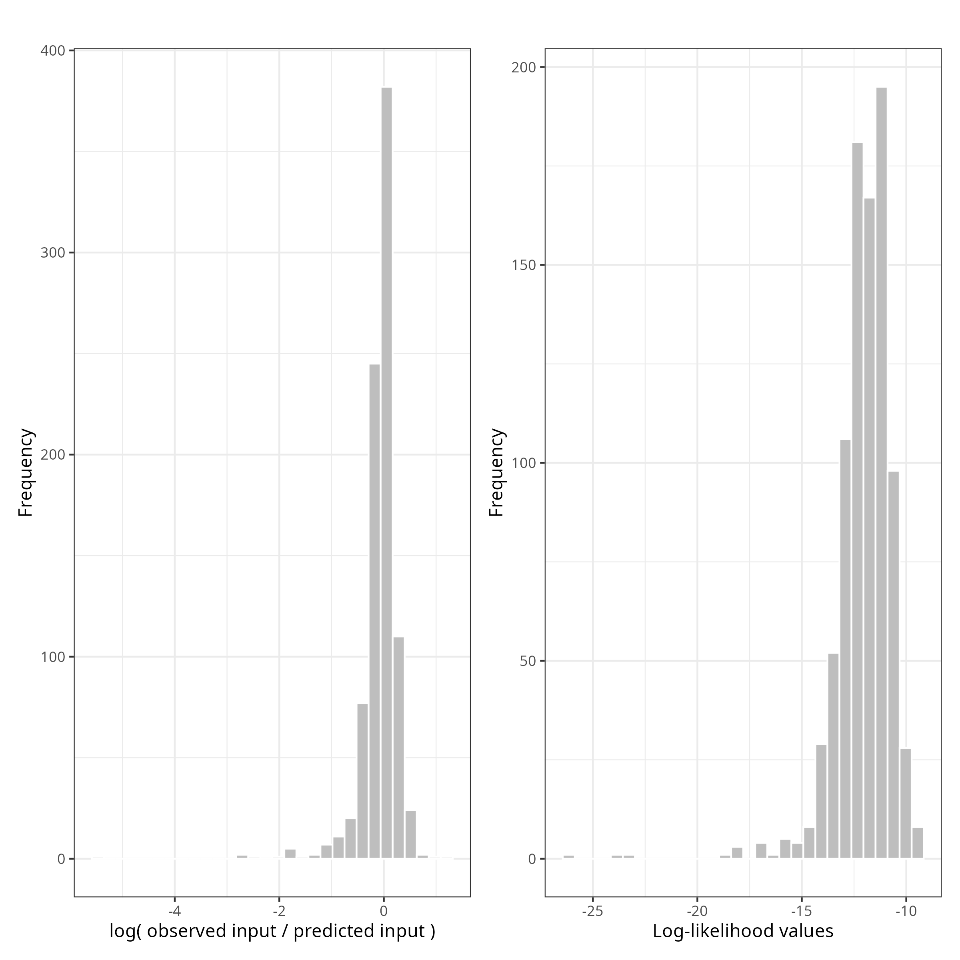
\includegraphics[
        width=1\textwidth,
        height=0.6\textheight
    ]{figures/hist_OMK_1_conv.png}
    \caption{Seed (OMK$_\text{1}$): log( observed input / predicted input ) = kind of residuals; log-likelihood values = kind of model 'fit'.}
    \label{fig:hist-OMK-1}
\end{figure}

\begin{figure}[htbp]
    \centering
    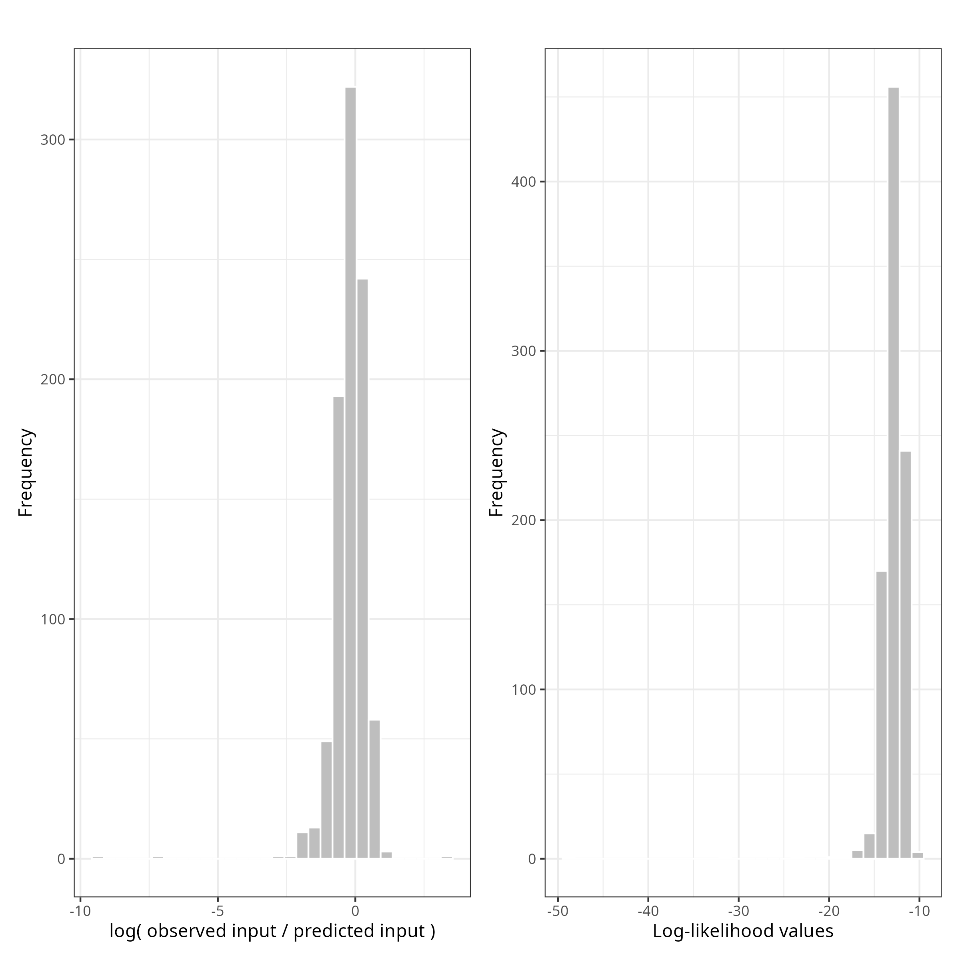
\includegraphics[
        width=1\textwidth,
        height=0.6\textheight
    ]{figures/hist_OMK_2_conv.png}
    \caption{Fertilisers (OMK$_\text{2}$): log( observed input / predicted input ) = kind of residuals; log-likelihood values = kind of model 'fit'.}
    \label{fig:hist-OMK-2}
\end{figure}

\begin{figure}[htbp]
    \centering
    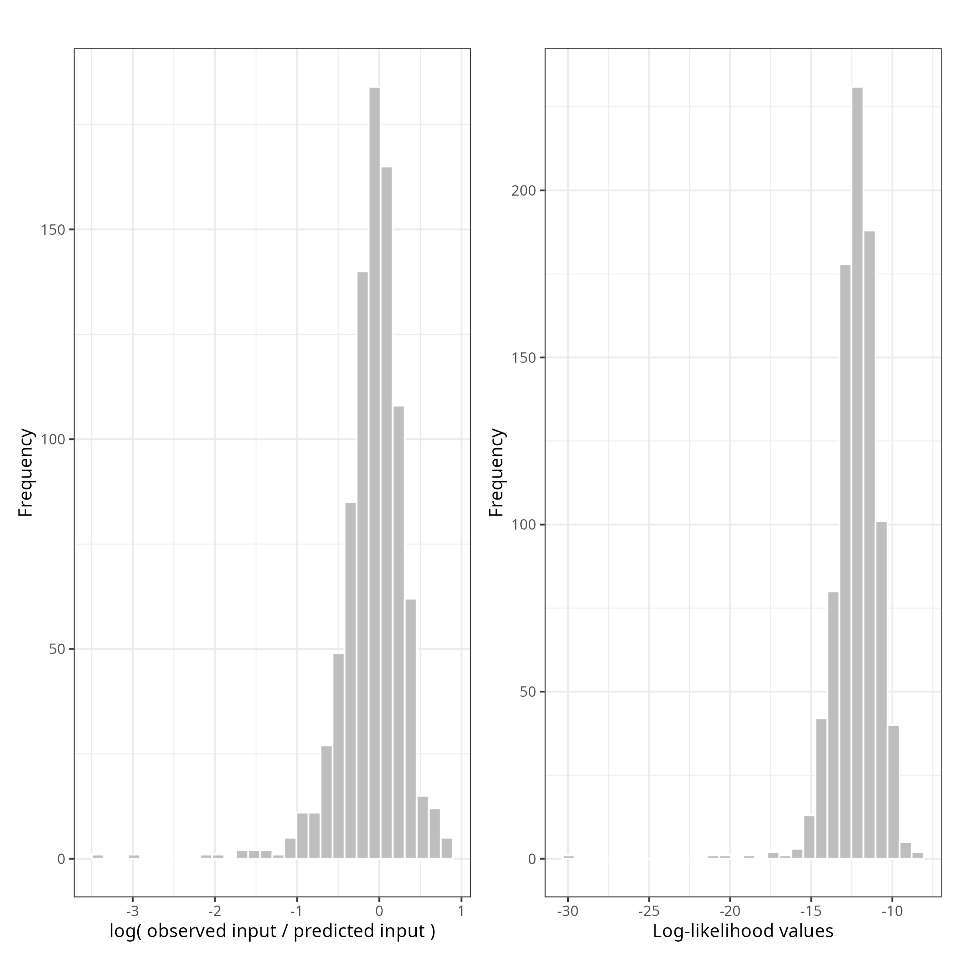
\includegraphics[
        width=1\textwidth,
        height=0.6\textheight
    ]{figures/hist_OMK_3_conv.png}
    \caption{Plant protection (OMK$_\text{3}$): log( observed input / predicted input ) = kind of residuals; log-likelihood values = kind of model 'fit'.}
    \label{fig:hist-OMK-3}
\end{figure}

\begin{figure}[htbp]
    \centering
    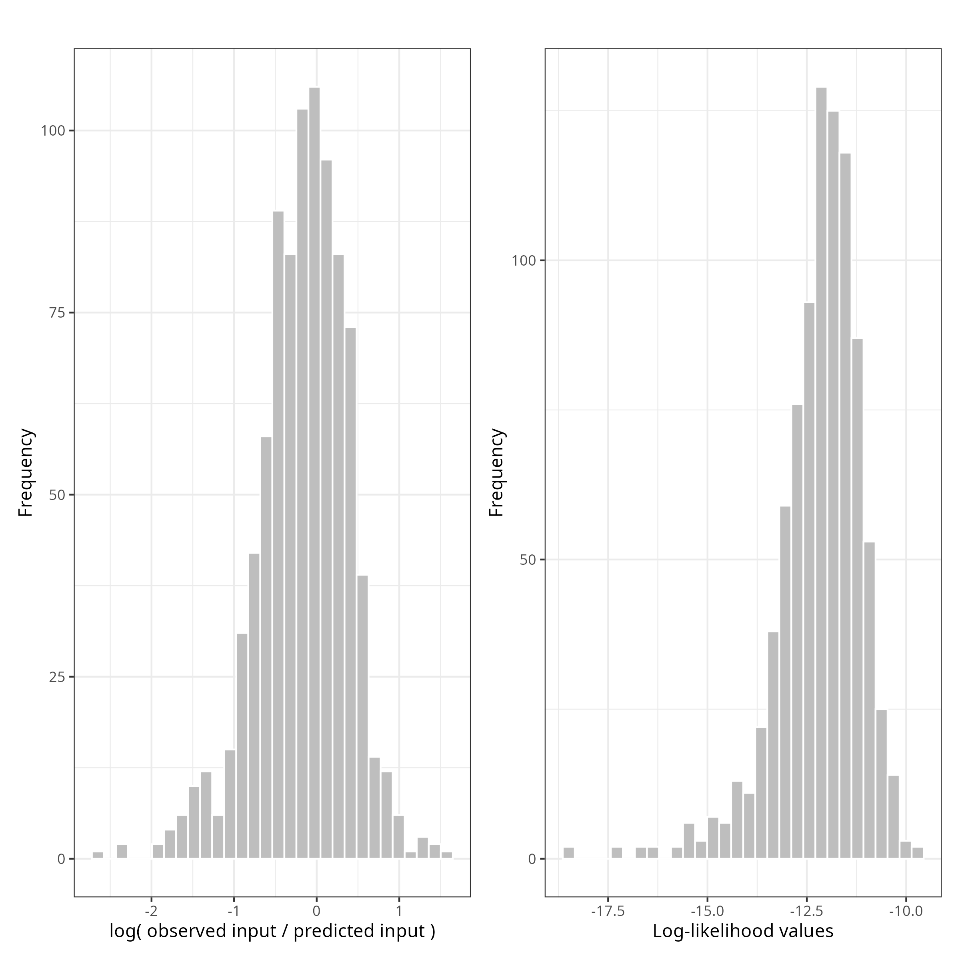
\includegraphics[
        width=1\textwidth,
        height=0.6\textheight
    ]{figures/hist_OMK_4_conv.png}
    \caption{Miscellaneous regarding field use (OMK$_\text{4}$): log( observed input / predicted input ) = kind of residuals; log-likelihood values = kind of model 'fit'.}
    \label{fig:hist-OMK-4}
\end{figure}

\begin{figure}[htbp]
    \centering
    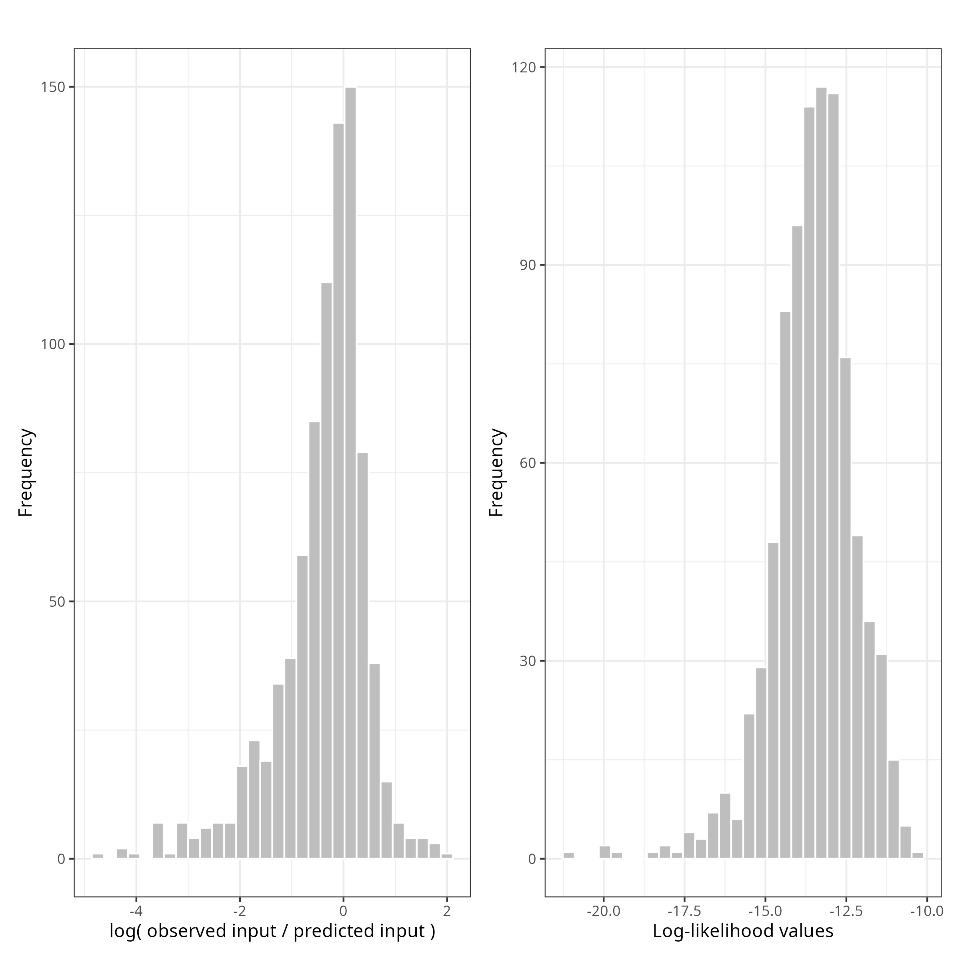
\includegraphics[
        width=1\textwidth,
        height=0.6\textheight
    ]{figures/hist_OMK_5_conv.png}
    \caption{Agricultural contractor services (OMK$_\text{5}$): log( observed input / predicted input ) = kind of residuals; log-likelihood values = kind of model 'fit'.}
    \label{fig:hist-OMK-5}
\end{figure}

\begin{figure}[htbp]
    \centering
    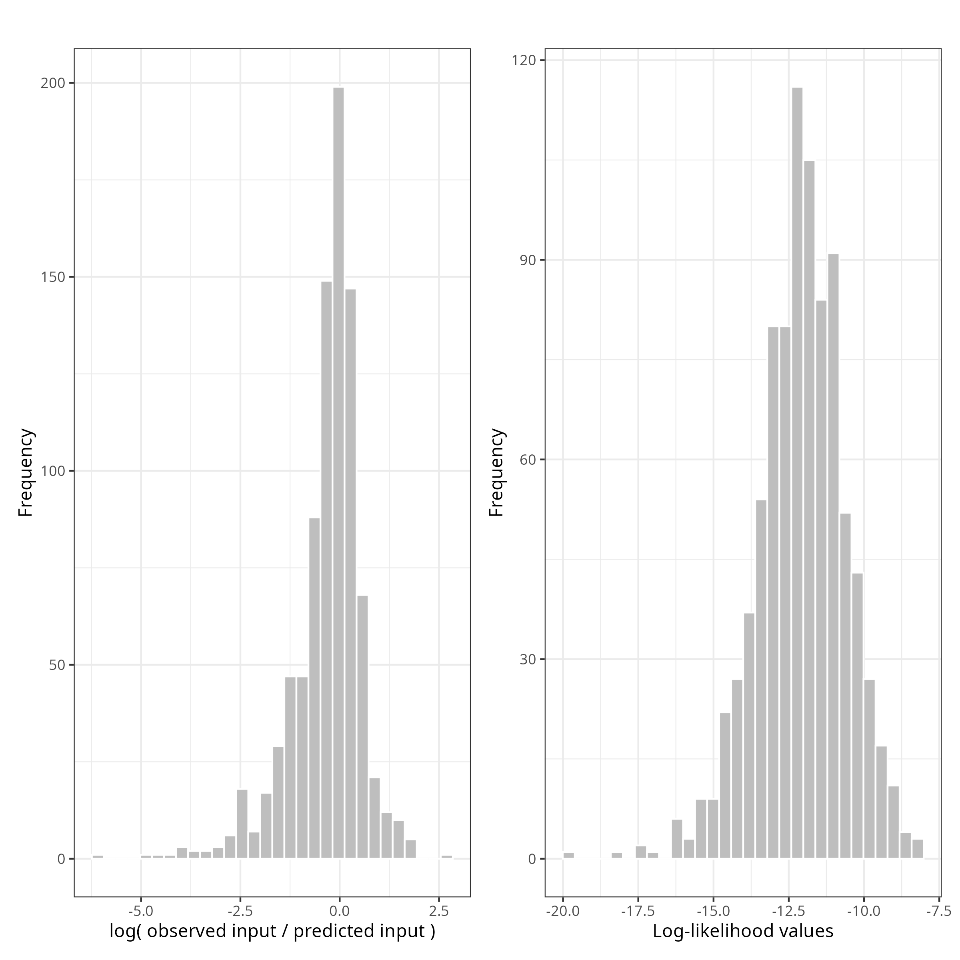
\includegraphics[
        width=1\textwidth,
        height=0.6\textheight
    ]{figures/hist_OMK_6_conv.png}
    \caption{Energy (OMK$_\text{6}$): log( observed input / predicted input ) = kind of residuals; log-likelihood values = kind of model 'fit'.}
    \label{fig:hist-OMK-6}
\end{figure}

\begin{figure}[htbp]
    \centering
    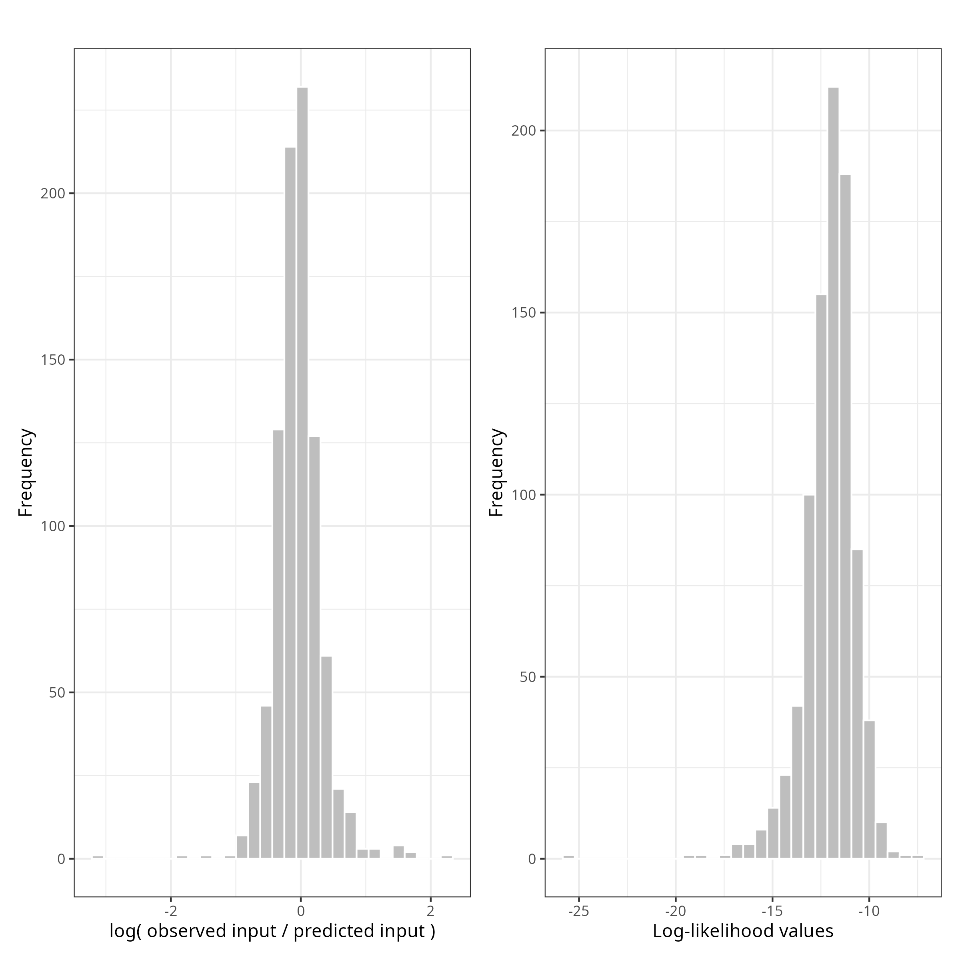
\includegraphics[
        width=1\textwidth,
        height=0.6\textheight
    ]{figures/hist_OMK_7_conv.png}
    \caption{Fuel (OMK$_\text{7}$): log( observed input / predicted input ) = kind of residuals; log-likelihood values = kind of model 'fit'.}
    \label{fig:hist-OMK-7}
\end{figure}

\begin{figure}[htbp]
    \centering
    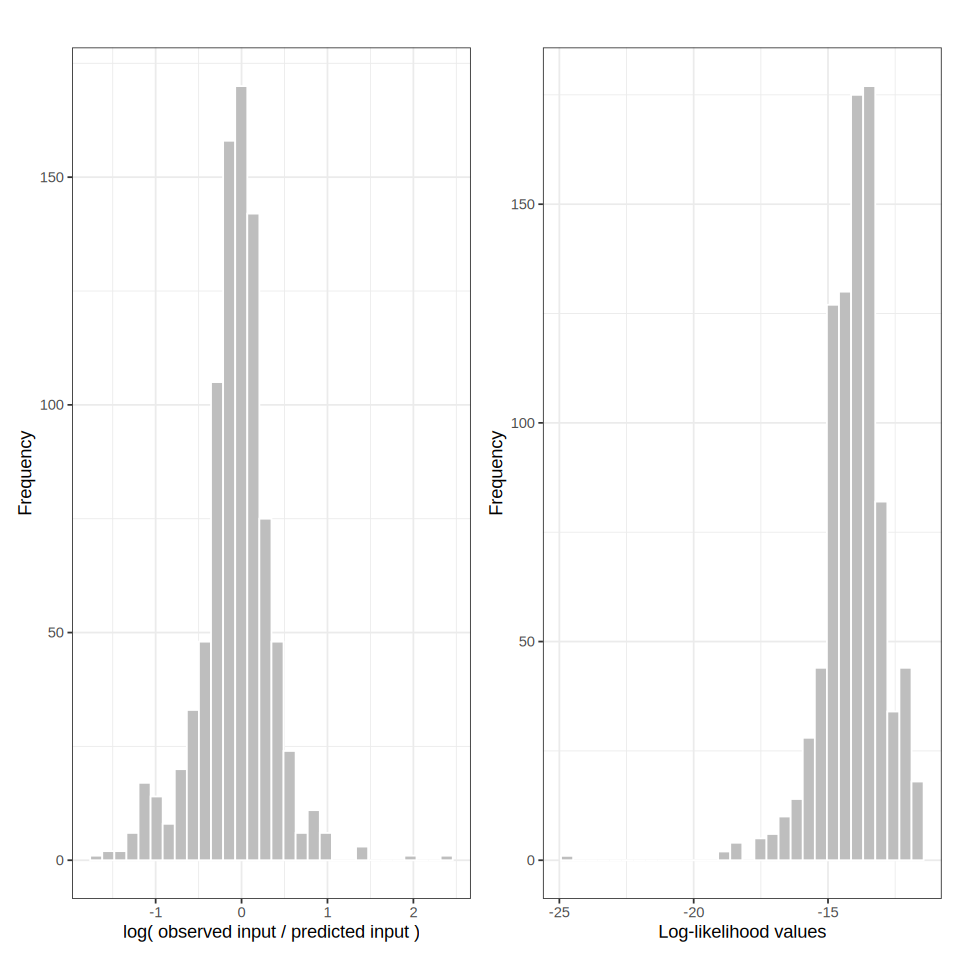
\includegraphics[
        width=1\textwidth,
        height=0.6\textheight
    ]{figures/hist_OMK_8_conv.png}
    \caption{Labor (OMK$_\text{8}$): log( observed input / predicted input ) = kind of residuals; log-likelihood values = kind of model 'fit'.}
    \label{fig:hist-OMK-8}
\end{figure}

\begin{figure}[htbp]
    \centering
    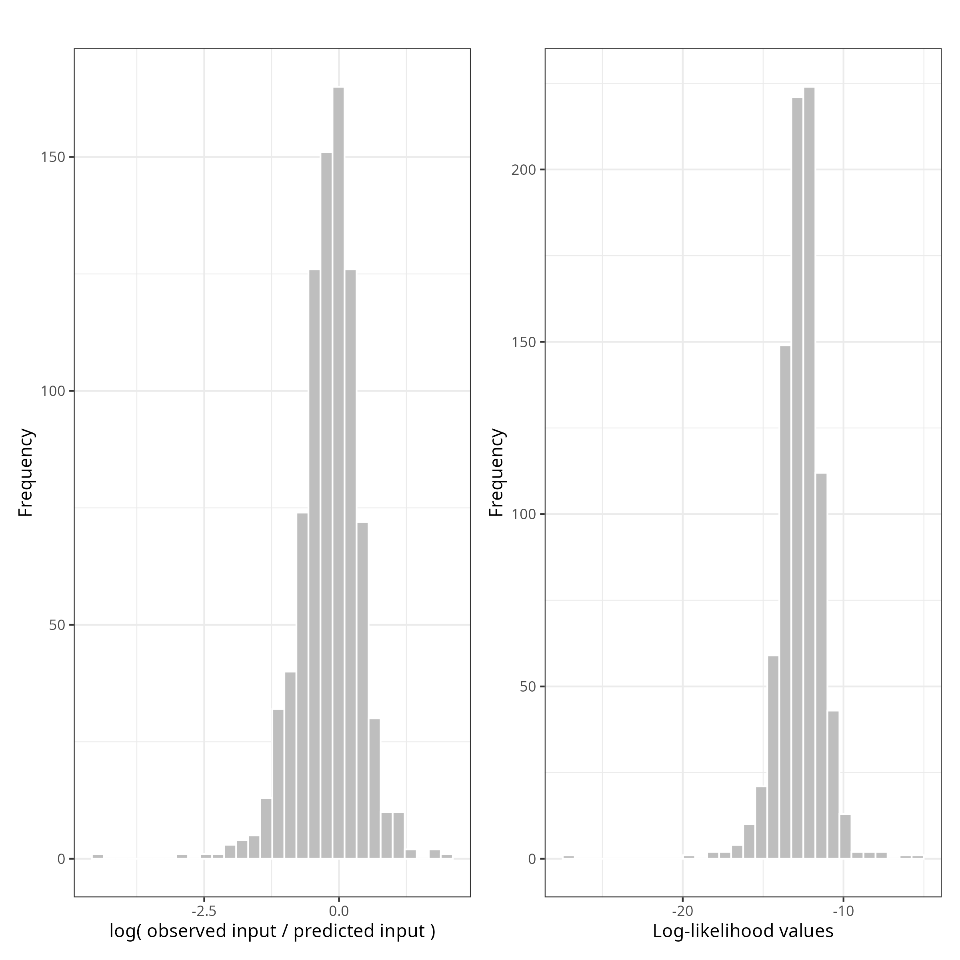
\includegraphics[
        width=1\textwidth,
        height=0.6\textheight
    ]{figures/hist_OMK_9_conv.png}
    \caption{Maintenance, fields (OMK$_\text{9}$): log( observed input / predicted input ) = kind of residuals; log-likelihood values = kind of model 'fit'.}
    \label{fig:hist-OMK-9}
\end{figure}

\begin{figure}[htbp]
    \centering
    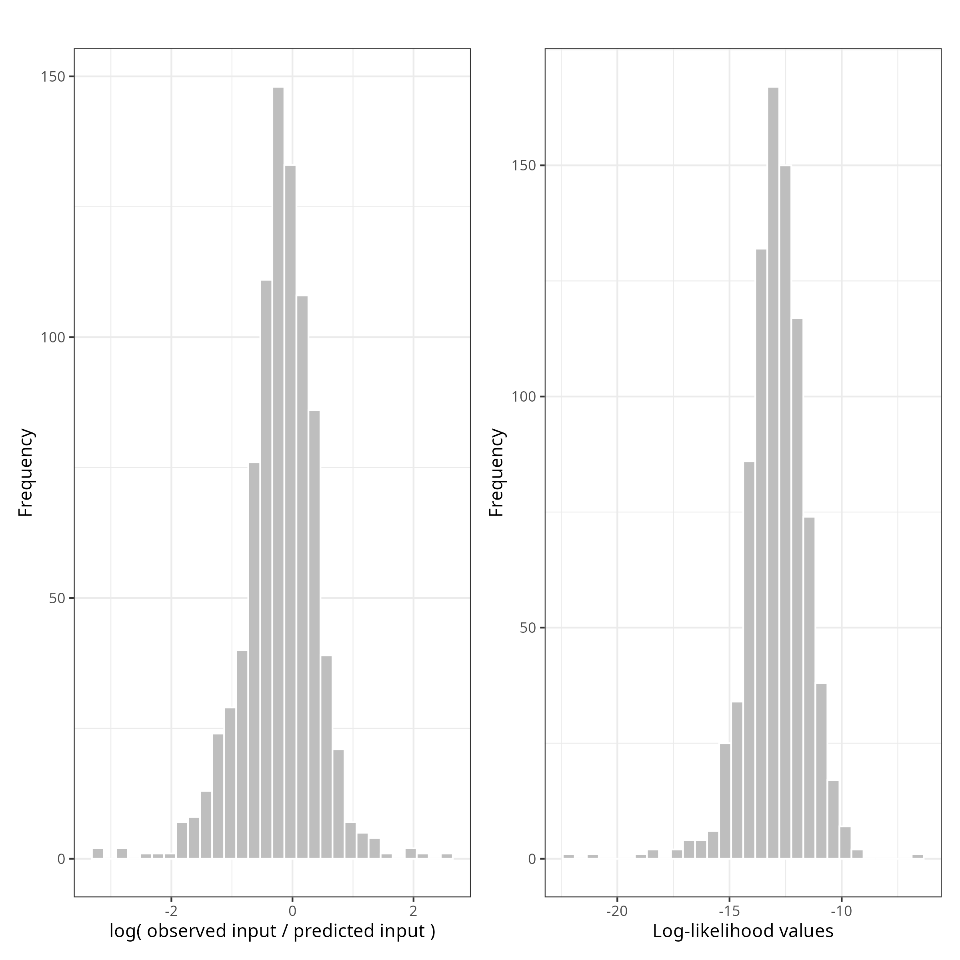
\includegraphics[
        width=1\textwidth,
        height=0.6\textheight
    ]{figures/hist_OMK_10_conv.png}
    \caption{Depreciations, fields (OMK$_\text{10}$): log( observed input / predicted input ) = kind of residuals; log-likelihood values = kind of model 'fit'.}
    \label{fig:hist-OMK-10}
\end{figure}



\newpage


\subsection{Tests}
\label{sec:test-results}

\begin{table}[htbp]
\centering
\caption{Hausman Tests for Fixed Effects}
\label{tab:fe-tests}
\begin{threeparttable}
\begin{tabular}{lrrr}
\toprule
Test & $\chi^2$ & $df$ & $p$-value \\
\midrule
\addlinespace
\multicolumn{4}{l}{\textit{Hausman tests}} \\
\text{ Catchment fixed effects} & 26.247 & 41 & 0.964 \\
\text{ Farm fixed effects}      & 65.171 & 41 & 0.010 \\
\addlinespace
\bottomrule
\end{tabular}
\begin{tablenotes}
\footnotesize
\item \textit{Notes:} The Hausman test evaluates whether the fixed effects
estimator is consistent relative to the pooling (no fixed effects) estimator,
under the null hypothesis that both estimators are consistent (i.e.\ fixed
effects are not needed). Rejection of the null indicates that the fixed
effects estimator is preferred. Catchment fixed effects are defined at the
level of the 11 coastal water catchments; Farm fixed effects are defined at
the CVR farm level ($n = 894$).
\end{tablenotes}
\end{threeparttable}
\end{table}

\begin{table}[htbp]
\centering
\small
\caption{Tests for Interaction Terms}
\label{tab:int-tests}
\begin{threeparttable}
\begin{tabular}{lrrr}
\toprule
Test & $df$ & $\chi^2$ & $p$-value \\
\midrule
\addlinespace
\text{ Model (1) vs. Model (3): CVR FE}     & 22 & 41.640 & 0.007 \\
\addlinespace
\text{ Model (2) vs. Model (4): No CVR FE}  & 22 & 47.009 & 0.001 \\
\addlinespace
\bottomrule
\end{tabular}
\begin{tablenotes}
\footnotesize
\item \textit{Notes:} The Wald tests compare the models \textit{with}
interaction terms against the models \textit{without} interaction terms,
testing the null hypothesis that the soil type effects are identical across
all crop categories. Model (1) and (2) include farm-level CVR fixed effects;
Model (3) and (4) do not. The test statistic is $\chi^2$-distributed under
the null hypothesis with 22 degrees of freedom, corresponding to the 22
additional interaction coefficients ($\mu_s \times \delta_{sk}$ for
$s \in \{1,2\}$ and $k = 1, \ldots, 11$ non-base crop categories).
\end{tablenotes}
\end{threeparttable}
\end{table}


\newpage


\subsection{OLS Estimation}
\label{sec:ols-method}
Given that our regression model in equation~(\ref{eq:est-model-spec-estimated}) complies with the Classical Linear Model assumptions, the OLS is a useful estimator as it allows conclusions to be drawn based on t-statistics and F-statistics.
To implement the farm-level fixed effects, we use the \texttt{plm} package in \texttt{R}.
Specifically, we construct a panel data frame with farm ID (\texttt{cvr}) as the individual index and crop category as the time index.
We then estimate equation~(\ref{eq:est-model-spec-estimated}) with \texttt{model = "within"} and \texttt{effect = "individual"}.
The within estimator subtracts for each farm $i$, the farm-specific mean from each observation.
This eliminates the farm fixed effects $\lambda_i$ from the estimating equation, which allows estimating the parameters without explicitly estimating $N-1$ farm intercepts. 



\subsubsection{Tables}
\label{sec:ols-estimation-tables}

%% Model 1: Interaction + CVR FE
\begin{longtable}{lrrr}
\caption{Revenue Model: Interaction Terms and Farm Fixed Effects}
\label{tab:model-int-fixed} \\
\toprule
Variable & Estimate & Std. Error & $p$-value \\
\midrule
\endfirsthead
\multicolumn{4}{l}{\textit{Table \ref{tab:model-int-fixed} continued}} \\
\toprule
Variable & Estimate & Std. Error & $p$-value \\
\midrule
\endhead
\midrule
\multicolumn{4}{r}{\textit{Continued on next page}} \\
\endfoot
\bottomrule
\endlastfoot
\multicolumn{4}{l}{\textit{Soil type shares (base: loamy soil)}} \\
\text{ Fine sand}                & $-$0.050 & 0.119 & 0.678 \\
\text{ Coarse sand}              & $+$0.004 & 0.167 & 0.980 \\
\addlinespace
\multicolumn{4}{l}{\textit{Crop category (base: wheat)}} \\
\text{ Barley}                   & $-$0.557 & 0.065 & $<$0.001 \\
\text{ Rye/Triticale}            & $-$0.160 & 0.075 & 0.034 \\
\text{ Seeds}                    & $+$0.057 & 0.089 & 0.524 \\
\text{ Oats/Mixed grain}         & $-$0.218 & 0.099 & 0.027 \\
\text{ Rapeseed}                 & $+$0.265 & 0.061 & $<$0.001 \\
\text{ Potatoes}                 & $+$1.960 & 0.143 & $<$0.001 \\
\text{ Legumes}                  & $-$0.332 & 0.159 & 0.036 \\
\text{ Sugar beet}               & $+$0.638 & 0.187 & 0.001 \\
\text{ Roughage}                 & $-$2.014 & 0.107 & $<$0.001 \\
\text{ Energy crops}             & $+$1.238 & 0.368 & 0.001 \\
\text{ Fodder maize}             & $-$0.014 & 0.092 & 0.877 \\
\addlinespace
\multicolumn{4}{l}{\textit{Crop sub-category shares}} \\
\text{ Winter barley}            & $+$0.502 & 0.134 & $<$0.001 \\
\text{ Fava beans}               & $+$0.330 & 0.167 & 0.048 \\
\text{ Early/seed potatoes}      & $+$0.334 & 0.416 & 0.422 \\
\text{ Consumption potatoes}     & $-$0.545 & 0.254 & 0.032 \\
\text{ Horticultural seeds}      & $+$0.863 & 0.252 & 0.001 \\
\text{ Spring wheat}             & $-$0.307 & 0.286 & 0.283 \\
\addlinespace
\multicolumn{4}{l}{\textit{Soil $\times$ crop interactions (base: wheat)}} \\
\text{ Fine sand $\times$ Legumes}            & $-$0.053 & 0.256 & 0.837 \\
\text{ Fine sand $\times$ Barley}             & $+$0.182 & 0.169 & 0.283 \\
\text{ Fine sand $\times$ Energy crops}       & $-$2.222 & 0.572 & $<$0.001 \\
\text{ Fine sand $\times$ Fodder maize}       & $+$0.146 & 0.228 & 0.522 \\
\text{ Fine sand $\times$ Seeds}              & $-$0.092 & 0.193 & 0.634 \\
\text{ Fine sand $\times$ Roughage}           & $+$1.006 & 0.277 & $<$0.001 \\
\text{ Fine sand $\times$ Oats/Mixed grain}   & $-$0.023 & 0.219 & 0.916 \\
\text{ Fine sand $\times$ Potatoes}           & $-$0.409 & 0.297 & 0.168 \\
\text{ Fine sand $\times$ Rapeseed}           & $+$0.006 & 0.158 & 0.972 \\
\text{ Fine sand $\times$ Rye/Triticale}      & $+$0.026 & 0.168 & 0.876 \\
\text{ Fine sand $\times$ Sugar beet}         & $+$0.155 & 0.320 & 0.628 \\
\text{ Coarse sand $\times$ Legumes}          & $-$0.048 & 0.409 & 0.906 \\
\text{ Coarse sand $\times$ Barley}           & $-$0.159 & 0.240 & 0.509 \\
\text{ Coarse sand $\times$ Energy crops}     & $-$2.735 & 1.905 & 0.151 \\
\text{ Coarse sand $\times$ Fodder maize}     & $-$0.097 & 0.344 & 0.778 \\
\text{ Coarse sand $\times$ Seeds}            & $+$0.100 & 0.292 & 0.731 \\
\text{ Coarse sand $\times$ Roughage}         & $+$0.428 & 0.391 & 0.274 \\
\text{ Coarse sand $\times$ Oats/Mixed grain} & $+$0.055 & 0.292 & 0.849 \\
\text{ Coarse sand $\times$ Potatoes}         & $-$0.169 & 0.391 & 0.666 \\
\text{ Coarse sand $\times$ Rapeseed}         & $-$0.187 & 0.239 & 0.435 \\
\text{ Coarse sand $\times$ Rye/Triticale}    & $-$0.182 & 0.244 & 0.455 \\
\text{ Coarse sand $\times$ Sugar beet}       & $-$0.243 & 0.405 & 0.549 \\
\addlinespace
\multicolumn{4}{l}{\textit{Model fit}} \\
Observations        & \multicolumn{3}{l}{3,232} \\
$n$ (farms)         & \multicolumn{3}{l}{894} \\
Residual Sum of Squares & \multicolumn{3}{l}{848.24} \\
$R^2$               & \multicolumn{3}{l}{0.542} \\
Adjusted $R^2$      & \multicolumn{3}{l}{0.355} \\
Farm fixed effects  & \multicolumn{3}{l}{Yes} \\
\end{longtable}

\newpage

%% Model 2: Interaction + No CVR FE
\begin{longtable}{lrrr}
\caption{Revenue Model: Interaction Terms, No Farm Fixed Effects}
\label{tab:model-int-nofixed} \\
\toprule
Variable & Estimate & Std. Error & $p$-value \\
\midrule
\endfirsthead
\multicolumn{4}{l}{\textit{Table \ref{tab:model-int-nofixed} continued}} \\
\toprule
Variable & Estimate & Std. Error & $p$-value \\
\midrule
\endhead
\midrule
\multicolumn{4}{r}{\textit{Continued on next page}} \\
\endfoot
\bottomrule
\endlastfoot
\multicolumn{4}{l}{\textit{Intercept}} \\
\text{ (Intercept)}              & $+$9.157 & 0.041 & $<$0.001 \\
\addlinespace
\multicolumn{4}{l}{\textit{Soil type shares (base: loamy soil)}} \\
\text{ Fine sand}                & $-$0.076 & 0.105 & 0.473 \\
\text{ Coarse sand}              & $-$0.155 & 0.148 & 0.294 \\
\addlinespace
\multicolumn{4}{l}{\textit{Crop category (base: wheat)}} \\
\text{ Barley}                   & $-$0.584 & 0.059 & $<$0.001 \\
\text{ Rye/Triticale}            & $-$0.165 & 0.070 & 0.018 \\
\text{ Seeds}                    & $+$0.071 & 0.082 & 0.387 \\
\text{ Oats/Mixed grain}         & $-$0.233 & 0.091 & 0.010 \\
\text{ Rapeseed}                 & $+$0.252 & 0.057 & $<$0.001 \\
\text{ Potatoes}                 & $+$1.869 & 0.129 & $<$0.001 \\
\text{ Legumes}                  & $-$0.367 & 0.148 & 0.013 \\
\text{ Sugar beet}               & $+$0.702 & 0.165 & $<$0.001 \\
\text{ Roughage}                 & $-$1.966 & 0.090 & $<$0.001 \\
\text{ Energy crops}             & $+$1.496 & 0.343 & $<$0.001 \\
\text{ Fodder maize}             & $-$0.083 & 0.078 & 0.287 \\
\addlinespace
\multicolumn{4}{l}{\textit{Crop sub-category shares}} \\
\text{ Winter barley}            & $+$0.546 & 0.116 & $<$0.001 \\
\text{ Fava beans}               & $+$0.336 & 0.155 & 0.030 \\
\text{ Early/seed potatoes}      & $+$0.579 & 0.326 & 0.076 \\
\text{ Consumption potatoes}     & $-$0.424 & 0.223 & 0.057 \\
\text{ Horticultural seeds}      & $+$0.845 & 0.228 & $<$0.001 \\
\text{ Spring wheat}             & $-$0.648 & 0.241 & 0.007 \\
\addlinespace
\multicolumn{4}{l}{\textit{Soil $\times$ crop interactions (base: wheat)}} \\
\text{ Fine sand $\times$ Legumes}            & $-$0.125 & 0.240 & 0.602 \\
\text{ Fine sand $\times$ Barley}             & $+$0.181 & 0.151 & 0.231 \\
\text{ Fine sand $\times$ Energy crops}       & $-$2.472 & 0.537 & $<$0.001 \\
\text{ Fine sand $\times$ Fodder maize}       & $+$0.266 & 0.198 & 0.179 \\
\text{ Fine sand $\times$ Seeds}              & $-$0.028 & 0.176 & 0.874 \\
\text{ Fine sand $\times$ Roughage}           & $+$0.872 & 0.241 & $<$0.001 \\
\text{ Fine sand $\times$ Oats/Mixed grain}   & $-$0.065 & 0.199 & 0.746 \\
\text{ Fine sand $\times$ Potatoes}           & $-$0.129 & 0.270 & 0.633 \\
\text{ Fine sand $\times$ Rapeseed}           & $+$0.028 & 0.141 & 0.842 \\
\text{ Fine sand $\times$ Rye/Triticale}      & $-$0.006 & 0.153 & 0.971 \\
\text{ Fine sand $\times$ Sugar beet}         & $-$0.087 & 0.284 & 0.761 \\
\text{ Coarse sand $\times$ Legumes}          & $+$0.172 & 0.376 & 0.648 \\
\text{ Coarse sand $\times$ Barley}           & $-$0.021 & 0.213 & 0.923 \\
\text{ Coarse sand $\times$ Energy crops}     & $-$3.242 & 1.790 & 0.070 \\
\text{ Coarse sand $\times$ Fodder maize}     & $+$0.184 & 0.295 & 0.534 \\
\text{ Coarse sand $\times$ Seeds}            & $+$0.036 & 0.265 & 0.893 \\
\text{ Coarse sand $\times$ Roughage}         & $+$0.614 & 0.345 & 0.075 \\
\text{ Coarse sand $\times$ Oats/Mixed grain} & $+$0.156 & 0.264 & 0.556 \\
\text{ Coarse sand $\times$ Potatoes}         & $-$0.025 & 0.356 & 0.945 \\
\text{ Coarse sand $\times$ Rapeseed}         & $+$0.070 & 0.213 & 0.743 \\
\text{ Coarse sand $\times$ Rye/Triticale}    & $-$0.030 & 0.222 & 0.891 \\
\text{ Coarse sand $\times$ Sugar beet}       & $-$0.192 & 0.366 & 0.600 \\
\addlinespace
\multicolumn{4}{l}{\textit{Model fit}} \\
Observations        & \multicolumn{3}{l}{3,232} \\
$n$ (farms)         & \multicolumn{3}{l}{894} \\
Residual Sum of Squares & \multicolumn{3}{l}{1,280.7} \\
$R^2$               & \multicolumn{3}{l}{0.509} \\
Adjusted $R^2$      & \multicolumn{3}{l}{0.503} \\
Farm fixed effects  & \multicolumn{3}{l}{No} \\
\end{longtable}

\newpage

%% Model 3: No Interaction + CVR FE
\begin{longtable}{lrrr}
\caption{Revenue Model: No Interaction Terms, Farm Fixed Effects}
\label{tab:model-noint-fixed} \\
\toprule
Variable & Estimate & Std. Error & $p$-value \\
\midrule
\endfirsthead
\multicolumn{4}{l}{\textit{Table \ref{tab:model-noint-fixed} continued}} \\
\toprule
Variable & Estimate & Std. Error & $p$-value \\
\midrule
\endhead
\midrule
\multicolumn{4}{r}{\textit{Continued on next page}} \\
\endfoot
\bottomrule
\endlastfoot
\multicolumn{4}{l}{\textit{Soil type shares (base: loamy soil)}} \\
\text{ Fine sand}                & $-$0.015 & 0.048 & 0.751 \\
\text{ Coarse sand}              & $-$0.072 & 0.072 & 0.315 \\
\addlinespace
\multicolumn{4}{l}{\textit{Crop category (base: wheat)}} \\
\text{ Barley}                   & $-$0.527 & 0.039 & $<$0.001 \\
\text{ Rye/Triticale}            & $-$0.173 & 0.047 & $<$0.001 \\
\text{ Seeds}                    & $+$0.040 & 0.062 & 0.517 \\
\text{ Oats/Mixed grain}         & $-$0.211 & 0.065 & 0.001 \\
\text{ Rapeseed}                 & $+$0.248 & 0.038 & $<$0.001 \\
\text{ Potatoes}                 & $+$1.820 & 0.084 & $<$0.001 \\
\text{ Legumes}                  & $-$0.376 & 0.130 & 0.004 \\
\text{ Sugar beet}               & $+$0.658 & 0.114 & $<$0.001 \\
\text{ Roughage}                 & $-$1.691 & 0.054 & $<$0.001 \\
\text{ Energy crops}             & $+$0.109 & 0.196 & 0.580 \\
\text{ Fodder maize}             & $+$0.025 & 0.053 & 0.631 \\
\addlinespace
\multicolumn{4}{l}{\textit{Crop sub-category shares}} \\
\text{ Winter barley}            & $+$0.479 & 0.134 & $<$0.001 \\
\text{ Fava beans}               & $+$0.355 & 0.166 & 0.033 \\
\text{ Early/seed potatoes}      & $+$0.316 & 0.417 & 0.448 \\
\text{ Consumption potatoes}     & $-$0.487 & 0.244 & 0.046 \\
\text{ Horticultural seeds}      & $+$0.879 & 0.251 & $<$0.001 \\
\text{ Spring wheat}             & $-$0.242 & 0.286 & 0.397 \\
\addlinespace
\multicolumn{4}{l}{\textit{Model fit}} \\
Observations        & \multicolumn{3}{l}{3,232} \\
$n$ (farms)         & \multicolumn{3}{l}{894} \\
Residual Sum of Squares & \multicolumn{3}{l}{863.61} \\
$R^2$               & \multicolumn{3}{l}{0.533} \\
Adjusted $R^2$      & \multicolumn{3}{l}{0.350} \\
Farm fixed effects  & \multicolumn{3}{l}{Yes} \\
\end{longtable}

\newpage

%% Model 4: No Interaction + No CVR FE
\begin{longtable}{lrrr}
\caption{Revenue Model: No Interaction Terms, No Farm Fixed Effects}
\label{tab:model-noint-nofixed} \\
\toprule
Variable & Estimate & Std. Error & $p$-value \\
\midrule
\endfirsthead
\multicolumn{4}{l}{\textit{Table \ref{tab:model-noint-nofixed} continued}} \\
\toprule
Variable & Estimate & Std. Error & $p$-value \\
\midrule
\endhead
\midrule
\multicolumn{4}{r}{\textit{Continued on next page}} \\
\endfoot
\bottomrule
\endlastfoot
\multicolumn{4}{l}{\textit{Intercept}} \\
\text{ (Intercept)}              & $+$9.139 & 0.029 & $<$0.001 \\
\addlinespace
\multicolumn{4}{l}{\textit{Soil type shares (base: loamy soil)}} \\
\text{ Fine sand}                & $-$0.025 & 0.042 & 0.545 \\
\text{ Coarse sand}              & $-$0.099 & 0.062 & 0.110 \\
\addlinespace
\multicolumn{4}{l}{\textit{Crop category (base: wheat)}} \\
\text{ Barley}                   & $-$0.544 & 0.037 & $<$0.001 \\
\text{ Rye/Triticale}            & $-$0.175 & 0.045 & $<$0.001 \\
\text{ Seeds}                    & $+$0.065 & 0.059 & 0.266 \\
\text{ Oats/Mixed grain}         & $-$0.229 & 0.062 & $<$0.001 \\
\text{ Rapeseed}                 & $+$0.266 & 0.039 & $<$0.001 \\
\text{ Potatoes}                 & $+$1.824 & 0.076 & $<$0.001 \\
\text{ Legumes}                  & $-$0.389 & 0.122 & 0.001 \\
\text{ Sugar beet}               & $+$0.628 & 0.102 & $<$0.001 \\
\text{ Roughage}                 & $-$1.670 & 0.046 & $<$0.001 \\
\text{ Energy crops}             & $+$0.257 & 0.186 & 0.167 \\
\text{ Fodder maize}             & $+$0.006 & 0.045 & 0.901 \\
\addlinespace
\multicolumn{4}{l}{\textit{Crop sub-category shares}} \\
\text{ Winter barley}            & $+$0.538 & 0.116 & $<$0.001 \\
\text{ Fava beans}               & $+$0.345 & 0.155 & 0.026 \\
\text{ Early/seed potatoes}      & $+$0.587 & 0.327 & 0.072 \\
\text{ Consumption potatoes}     & $-$0.391 & 0.214 & 0.068 \\
\text{ Horticultural seeds}      & $+$0.845 & 0.228 & $<$0.001 \\
\text{ Spring wheat}             & $-$0.638 & 0.241 & 0.008 \\
\addlinespace
\multicolumn{4}{l}{\textit{Model fit}} \\
Observations        & \multicolumn{3}{l}{3,232} \\
$n$ (farms)         & \multicolumn{3}{l}{894} \\
Residual Sum of Squares & \multicolumn{3}{l}{1,299.6} \\
$R^2$               & \multicolumn{3}{l}{0.502} \\
Adjusted $R^2$      & \multicolumn{3}{l}{0.499} \\
Farm fixed effects  & \multicolumn{3}{l}{No} \\
\end{longtable}


\begin{table}[htbp]
\centering
\small
\caption{Predicted relative revenues $(\%\Delta)$ --- Interaction Terms}
\label{tab:pred-relative-yields-int}
\begin{threeparttable}
\begin{tabular}{lrrrrrr}
\toprule
& \multicolumn{3}{c}{\textbf{Fixed Effects}} 
& \multicolumn{3}{c}{\textbf{No Fixed Effects}} \\
\cmidrule(lr){2-4} \cmidrule(lr){5-7}
Baseline = wheat & Fine & Coarse & Loamy & Fine & Coarse & Loamy \\
\midrule
\addlinespace
\text{ Barley}           & $-$34.6 & $-$50.9 & $-$42.7
                         & $-$38.0 & $-$53.2 & $-$44.2 \\
\text{ Rapeseed}         &    24.8 &     8.7 &    30.4
                         &    22.7 &    18.1 &    28.6 \\
\text{ Fodder maize}     &     8.6 & $-$10.2 & $-$1.4
                         &    11.4 & $-$5.2  & $-$7.9  \\
\text{ Rye/Triticale}    & $-$16.7 & $-$28.6 & $-$14.7
                         & $-$21.8 & $-$29.6 & $-$15.2 \\
\text{ Roughage}         & $-$65.3 & $-$79.4 & $-$86.7
                         & $-$68.9 & $-$77.8 & $-$86.0 \\
\text{ Seeds}            & $-$8.1  &    17.5 &     5.9
                         & $-$3.2  & $-$4.7  &     7.4 \\
\text{ Oats/Mixed grain} & $-$25.2 & $-$14.7 & $-$19.6
                         & $-$31.1 & $-$20.7 & $-$20.8 \\
\text{ Potatoes}         &   348.9 &   502.0 &   610.0
                         &   428.3 &   441.7 &   548.2 \\
\text{ Legumes}          & $-$35.2 & $-$31.4 & $-$28.3
                         & $-$43.3 & $-$29.5 & $-$30.7 \\
\text{ Sugar beet}       &   110.3 &    49.0 &    89.2
                         &    71.5 &    42.6 &   101.7 \\
\text{ Energy crops}     & $-$64.4 & $-$77.5 &   245.0
                         & $-$65.1 & $-$85.1 &   346.2 \\
\addlinespace
\bottomrule
\end{tabular}
\begin{tablenotes}
\footnotesize
\item \textit{Notes:} All predicted relative revenues are relative to wheat on loamy
soil, and measured in percentage changes, i.e.\ $(\nu_{sk} - 1) \times 100$.
\end{tablenotes}
\end{threeparttable}
\end{table}

\begin{table}[H]
\centering
\small
\caption{Predicted relative revenues $(\%\Delta)$ --- No Interaction Terms}
\label{tab:pred-relative-yields-noint}
\begin{threeparttable}
\begin{tabular}{lrrrrrr}
\toprule
& \multicolumn{3}{c}{\textbf{Fixed Effects}} 
& \multicolumn{3}{c}{\textbf{No Fixed Effects}} \\
\cmidrule(lr){2-4} \cmidrule(lr){5-7}
Baseline = wheat & Fine & Coarse & Loamy & Fine & Coarse & Loamy \\
\midrule
\addlinespace
\multicolumn{7}{l}{\textit{Soil type effects}} \\
\text{ All crop categories} & $-$1.5 & $-$6.9 &    0.0
                            & $-$2.5 & $-$9.4 &    0.0 \\
\addlinespace
\multicolumn{7}{l}{\textit{Crop intercepts}} \\
\text{ Barley}              & \multicolumn{3}{c}{$-$41.0}
                            & \multicolumn{3}{c}{$-$42.0} \\
\text{ Rapeseed}            & \multicolumn{3}{c}{28.2}
                            & \multicolumn{3}{c}{30.4} \\
\text{ Fodder maize}        & \multicolumn{3}{c}{2.6}
                            & \multicolumn{3}{c}{0.6} \\
\text{ Rye/Triticale}       & \multicolumn{3}{c}{$-$15.9}
                            & \multicolumn{3}{c}{$-$16.1} \\
\text{ Roughage}            & \multicolumn{3}{c}{$-$81.6}
                            & \multicolumn{3}{c}{$-$81.2} \\
\text{ Seeds}               & \multicolumn{3}{c}{4.1}
                            & \multicolumn{3}{c}{6.7} \\
\text{ Oats/Mixed grain}    & \multicolumn{3}{c}{$-$19.1}
                            & \multicolumn{3}{c}{$-$20.5} \\
\text{ Potatoes}            & \multicolumn{3}{c}{517.3}
                            & \multicolumn{3}{c}{519.4} \\
\text{ Legumes}             & \multicolumn{3}{c}{$-$31.4}
                            & \multicolumn{3}{c}{$-$32.2} \\
\text{ Sugar beet}          & \multicolumn{3}{c}{93.0}
                            & \multicolumn{3}{c}{87.4} \\
\text{ Energy crops}        & \multicolumn{3}{c}{11.5}
                            & \multicolumn{3}{c}{29.3} \\
\addlinespace
\bottomrule
\end{tabular}
\begin{tablenotes}
\footnotesize
\item \textit{Notes:} All predicted relative revenues are relative to wheat on loamy
soil, and measured in percentage changes. Soil type effects are constant across
all crop categories in the no-interaction model. Crop intercepts show
$(\exp(\alpha_k) - 1) \times 100$ for loamy soil only.
\end{tablenotes}
\end{threeparttable}
\end{table}



\newpage


\subsubsection{Figures}
\label{sec:results-ols-figures}


\begin{figure}[htbp]
    \centering
    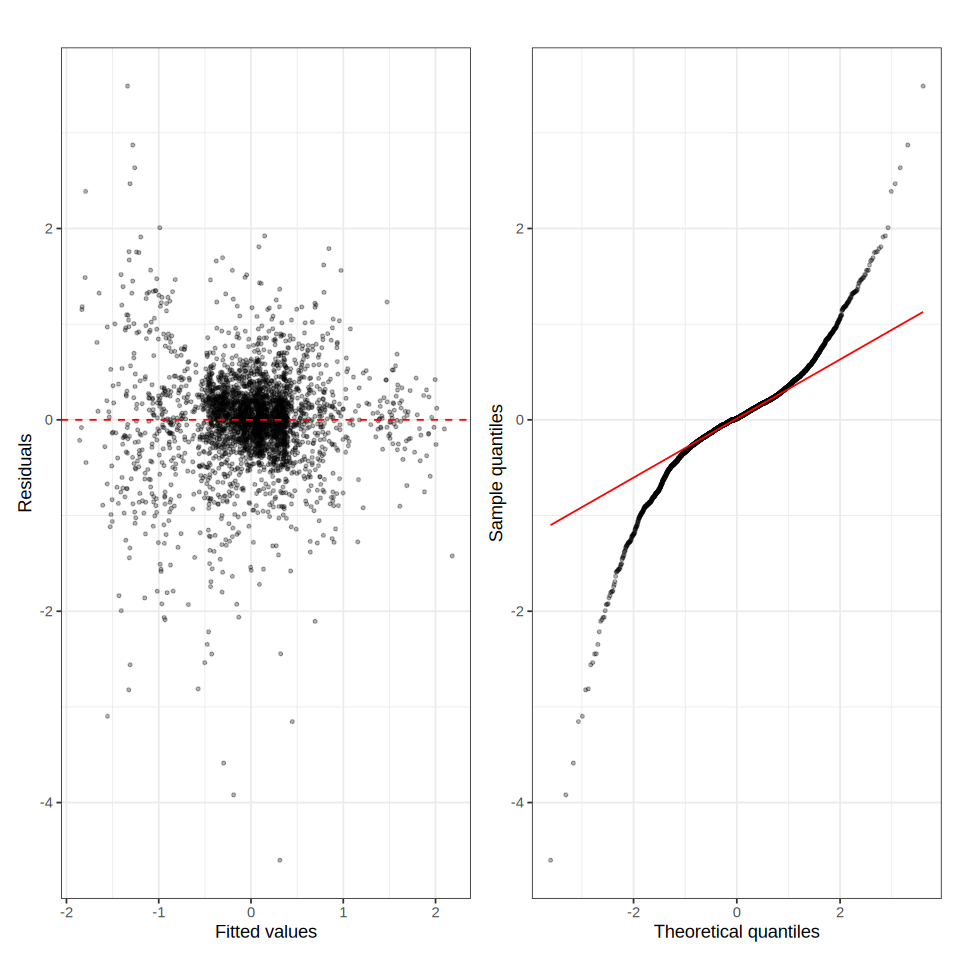
\includegraphics[
        width=1\textwidth,
        height=0.6\textheight
    ]{figures/figure_int_cvr.png}
    \caption{Residual Plot and Normal Q-Q plot of the Estimated Model (1): \textit{with} Interaction Terms and \textit{with} Farm-Level Fixed Effects.}
    \label{fig:resvsfit-int-cvr}
\end{figure}

\begin{figure}[htbp]
    \centering
    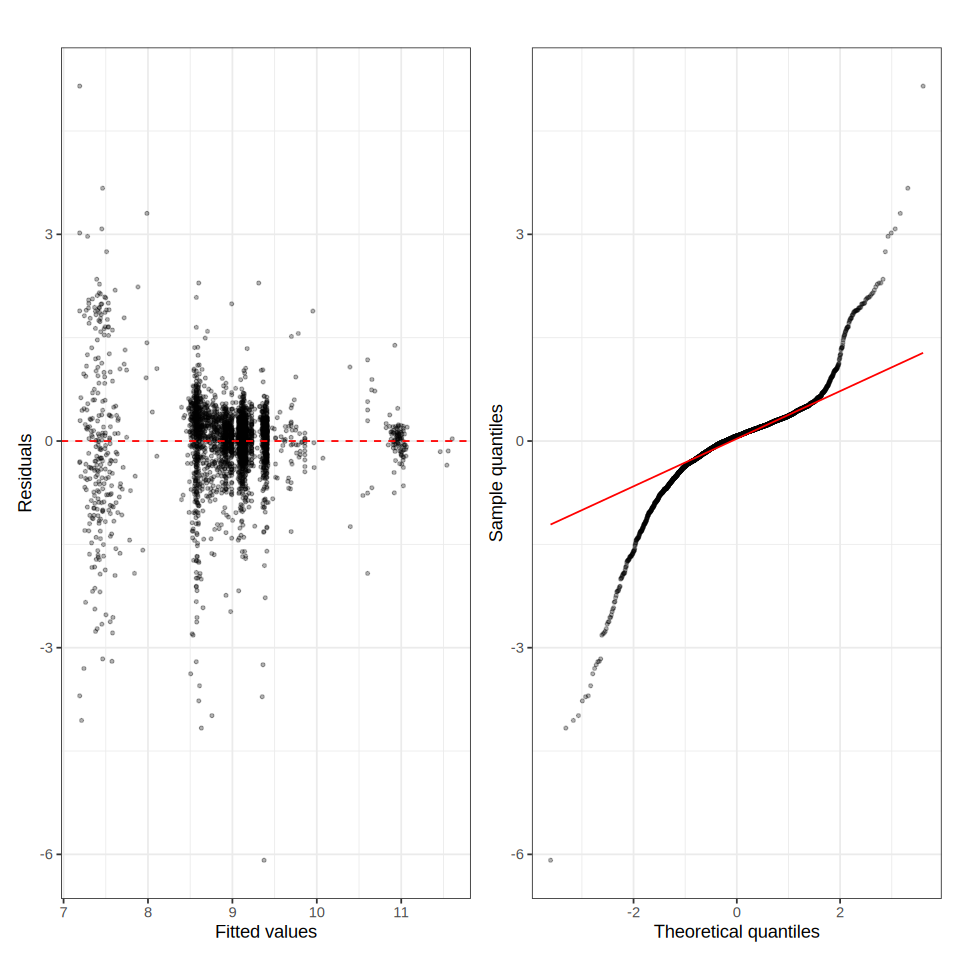
\includegraphics[
        width=1\textwidth,
        height=0.6\textheight
    ]{figures/figure_int_noCvr.png}
    \caption{Residual Plot and Normal Q-Q plot of the Estimated Model (2): \textit{with} Interaction Terms and \textit{without} Farm-Level Fixed Effects.}
    \label{fig:resvsfit-int-nocvr}
\end{figure}

\begin{figure}[htbp]
    \centering
    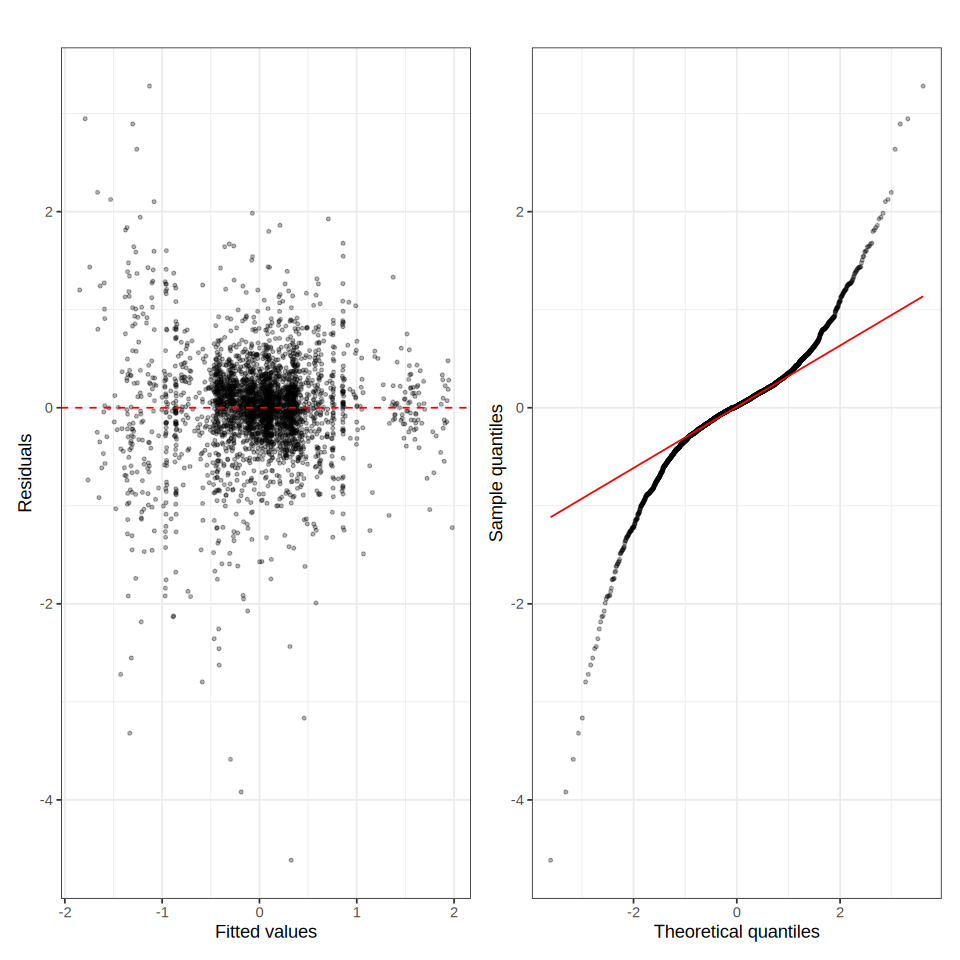
\includegraphics[
        width=1\textwidth,
        height=0.6\textheight
    ]{figures/figure_noInt_cvr.png}
    \caption{Residual Plot and Normal Q-Q plot of the Estimated Model (3): \textit{without} Interaction Terms and \textit{with} Farm-Level Fixed Effects.}
    \label{fig:resvsfit-noint-cvr}
\end{figure}

\begin{figure}[htbp]
    \centering
    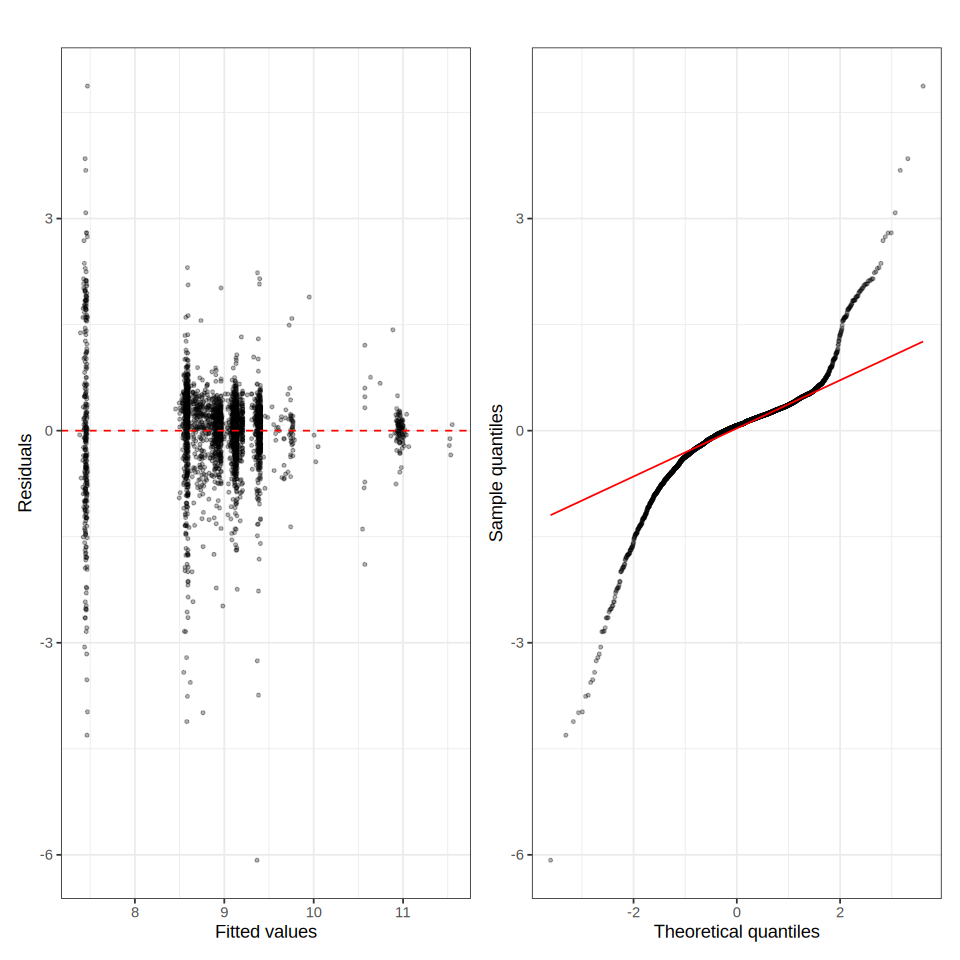
\includegraphics[
        width=1\textwidth,
        height=0.6\textheight
    ]{figures/figure_noInt_noCvr.png}
    \caption{Residual Plot and Normal Q-Q plot of the Estimated Model (4): \textit{without} Interaction Terms and \textit{without} Farm-Level Fixed Effects.}
    \label{fig:resvsfit-noint-nocvr}
\end{figure}



\newpage


\subsection{Validation}

\subsubsection{Tables}

\begin{table}[H]
\centering
\caption{Potential winter wheat farms to exclude in the analysis.}
\label{tab:outlier-robustness-wheat}
\begin{threeparttable}
\begin{tabular}{lccccc}
\toprule
Cutoff & High costs & Low costs & High revenue & Low revenue & Total (unique) \\
\midrule
$\pm 1$ SD   & 76 & 77 & 80 & 75 & 262 \\
$\pm 1.5$ SD & 38 & 18 & 29 & 38 & 111 \\
$\pm 2$ SD   & 22 &  4 & 14 & 16 & 52 \\
$\pm 3$ SD   &  8 & $-$ &  2 &  1 & 11 \\
\bottomrule
\end{tabular}
\begin{tablenotes}
\small
\item \textit{Notes:} 
The total (unique) column reports the potential number of unique farms to be excluded and is therefore not equal to the sum of the direction-specific columns.
The preferred specification uses $\pm 2$ standard deviations.
\end{tablenotes}
\end{threeparttable}
\end{table}

Table~\ref{tab:outlier-robustness-wheat} shows that the results are sensitive to the choice of cutoff at the lower end --- tightening the threshold to $\pm 1$ SD removes 262 unique farms, which risks excluding observations that reflect genuine heterogeneity rather than measurement error.
At the other extreme, $\pm 3$ SD retains all but 11 farms, which may be insufficient to remove the most problematic observations.
It should be noted that the direction-specific counts are not mutually exclusive --- a farm may simultaneously deviate in both costs and revenues, and is therefore counted in each relevant direction but only once in the unique total.


\begin{table}[H]
\centering
\caption{Potential spring barley farms to exclude in the analysis.}
\label{tab:outlier-robustness-barley}
\begin{threeparttable}
\begin{tabular}{lccccc}
\toprule
Cutoff & High costs & Low costs & High revenue & Low revenue & Total (unique) \\
\midrule
$\pm 1$ SD   & 95 & 82 & 51 & 81 & 278 \\
$\pm 1.5$ SD & 47 & 11 & 25 & 14 & 90 \\
$\pm 2$ SD   & 24 &  1 & 13 & $-$ & 36 \\
$\pm 3$ SD   &  10 & $-$ &  7 &  $-$ & 17 \\
\bottomrule
\end{tabular}
\begin{tablenotes}
\small
\item \textit{Notes:} 
The total (unique) column reports the potential number of unique farms to be excluded and is therefore not equal to the sum of the direction-specific columns.
The preferred specification uses $\pm 2$ standard deviations.
\end{tablenotes}
\end{threeparttable}
\end{table}



\subsubsection{Figures}

\begin{figure}[htbp]
    \centering
    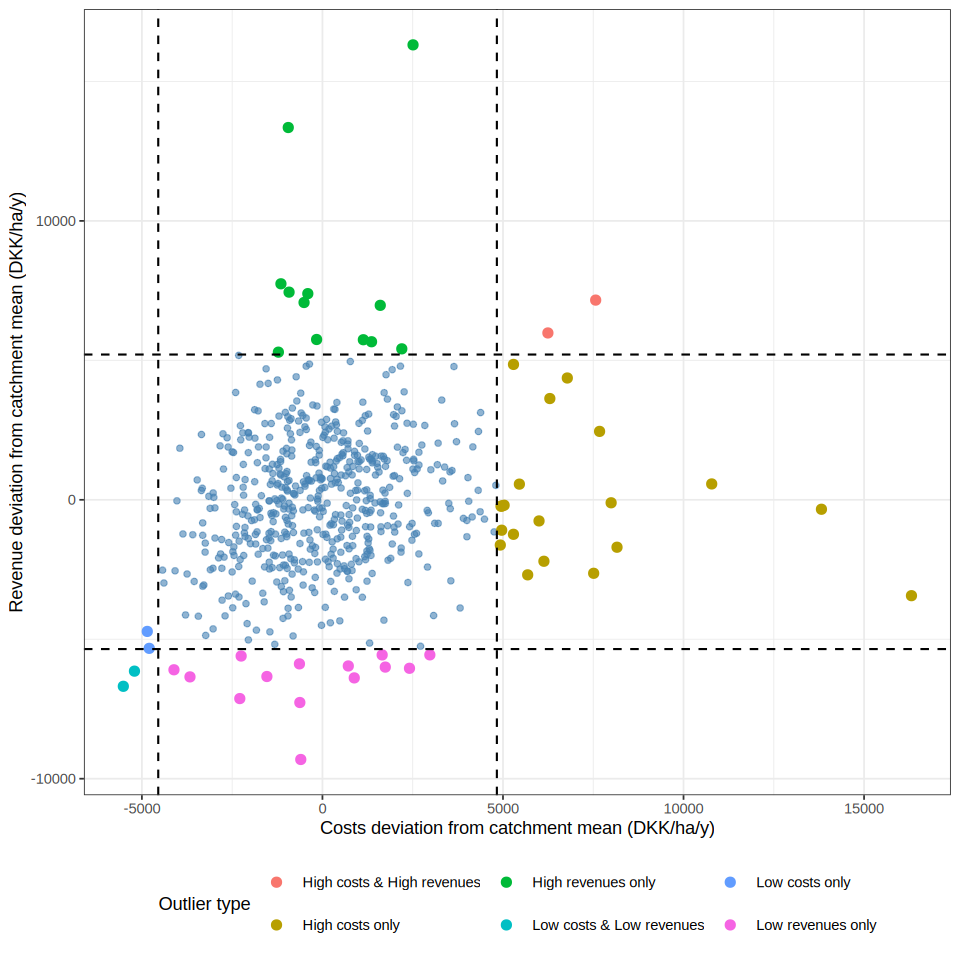
\includegraphics[
        width=0.9\textwidth,
        height=0.6\textheight
    ]{figures/scatterplot_outliers_hvede.png}
    \caption{Deviation of farm-level area-weighted average allocated revenues and costs per hectare from the catchment mean, for farms producing winter wheat (2024). 
    Each point represents one farm. 
    Dashed vertical lines indicate $\pm 2$ standard deviation cutoffs 
    for costs; dashed horizontal lines indicate $\pm 2$ standard 
    deviation cutoffs for revenues. Coloured points are flagged as 
    outliers and excluded from the analysis; blue points are retained.}
    \label{fig:outlier-identification-wheat}
\end{figure}


\begin{figure}[htbp]
    \centering
    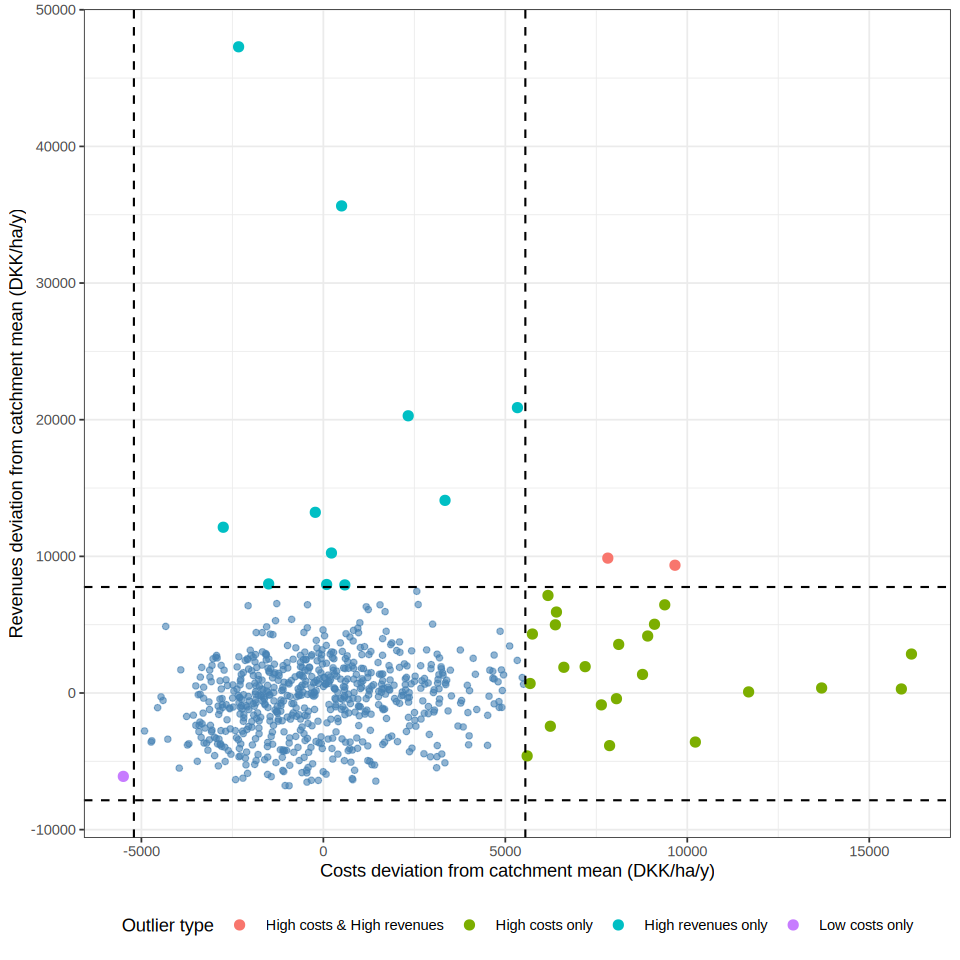
\includegraphics[
        width=0.9\textwidth,
        height=0.6\textheight
    ]{figures/scatterplot_outliers_byg.png}
    \caption{Deviation of farm-level area-weighted average allocated revenues and costs per hectare from the catchment mean, for farms producing spring barley (2024). 
    Each point represents one farm. 
    Dashed vertical lines indicate $\pm 2$ standard deviation cutoffs 
    for costs; dashed horizontal lines indicate $\pm 2$ standard 
    deviation cutoffs for revenues. Coloured points are flagged as 
    outliers and excluded from the analysis; blue points are retained.}
    \label{fig:outlier-identification-byg}
\end{figure}



\subsection{Profitability From Farmer's Perspective}
\label{sec:app-profitability-farmer}

\begin{table}[H]
\centering
\small
\caption{Average profitability (DKK/ha/y) for spring barley fields by 
catchment and soil type}
\label{tab:dbii-vaarbyg-convcrops}
\begin{threeparttable}
\begin{tabular}{lrrrrr}
\toprule
\textbf{Catchment} & \textbf{Fields} & \textbf{DBII} &
\textbf{Fine} & \textbf{Coarse} & \textbf{Loamy} \\
\midrule\addlinespace
Lister Dyb                 & 150 & $-$4,127 & $-$3,895 (36)  & $-$5,143 (22)  & $-$3,976 (92)  \\
Nissum Bredning            & 116 & $-$2,605 & $-$2,325 (20)  & $-$            & $-$2,727 (79)  \\
Nissum Fjord, Felsted Kog  & 443 &   $-$513 &    $+$89 (125) &  $-$801 (89)   &  $-$740 (229)  \\
Thisted Bredning           &  75 & $-$1,896 & $-$            & $-$            & $-$2,107 (48)  \\
Nibe Bredning og Langerak  & 433 &   $-$558 &    $+$27 (174) & $-$1,025 (68)  &  $-$964 (191)  \\
Randers Fjord, indre       & 354 & $-$1,704 & $-$1,929 (69)  & $-$1,767 (48)  & $-$1,640 (237) \\
Horsens Fjord, indre       &  46 & $-$3,120 & $-$            & $-$            & $-$3,147 (32)  \\
Odense Fjord, Seden Strand &  70 & $-$1,729 & $-$            & $-$            & $-$1,258 (49)  \\
Isefjord, indre            &  61 & $-$3,295 & $-$            & $-$            & $-$3,061 (43)  \\
Karrebæk Fjord             & 177 & $-$3,192 & $-$3,261 (38)  & $-$3,514 (21)  & $-$3,134 (118) \\
Roskilde Fjord, indre      &  52 & $-$3,536 & $-$            & $-$            & $-$3,456 (33)  \\
\addlinespace\bottomrule
\end{tabular}
\begin{tablenotes}
\footnotesize
\item \textit{Notes:} All values are measured in DKK per hectare and 
weighted by area; DBII denotes gross margin II; Fine, Coarse, and 
Loamy refer to DBII for fields on the respective soil type within 
each catchment; numbers in parentheses indicate the number of fields; 
`$-$' indicates fewer than 20 fields and is therefore not reported.
\end{tablenotes}
\end{threeparttable}
\end{table}

\subsection{Winter Wheat Reference Scenario}
\subsubsection{Field-level Distribution of Damage Costs}
\label{Field-level Distribution of Damage Costs}

\begin{figure}[H]
\centering
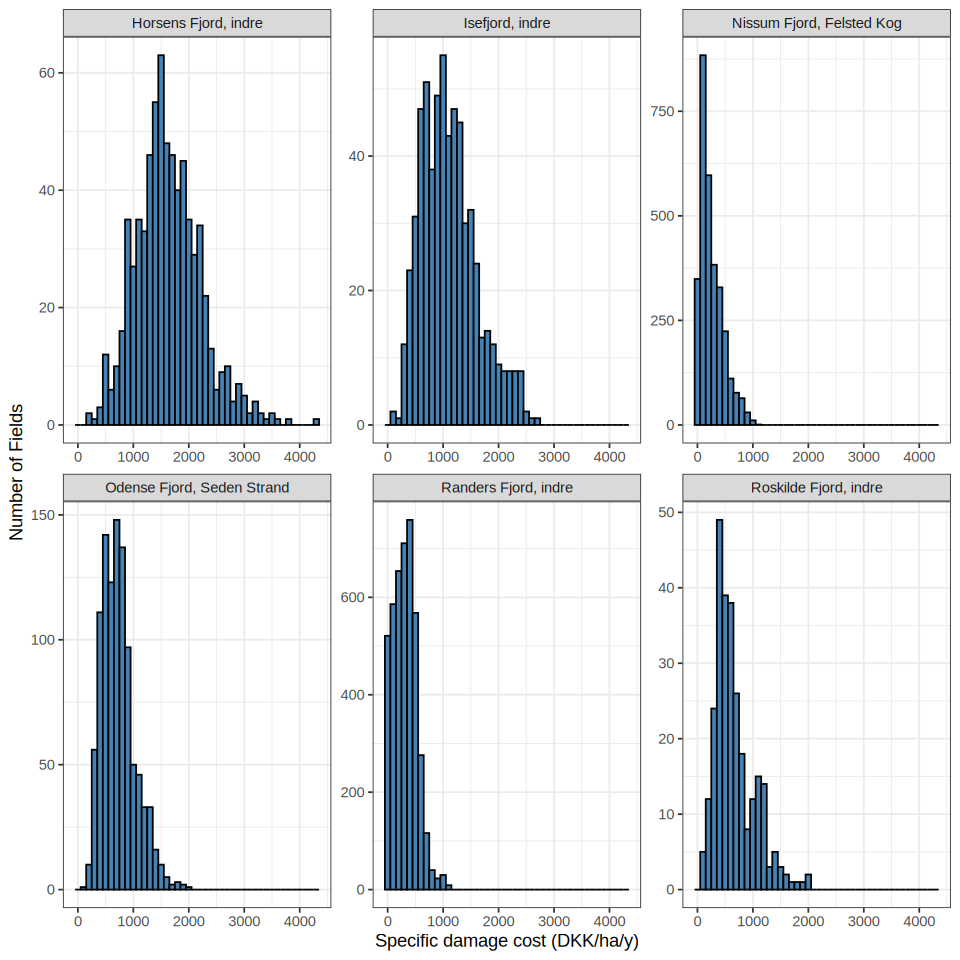
\includegraphics[width=0.8\textwidth]{figures/hist_specific_dcost_hvede.png}
\caption{Distribution of Specific Damage Cost (DKK/ha/y) - Winter wheat.}
\label{fig:hist_DC_spec_all}
\end{figure}

\begin{figure}[H]
\centering
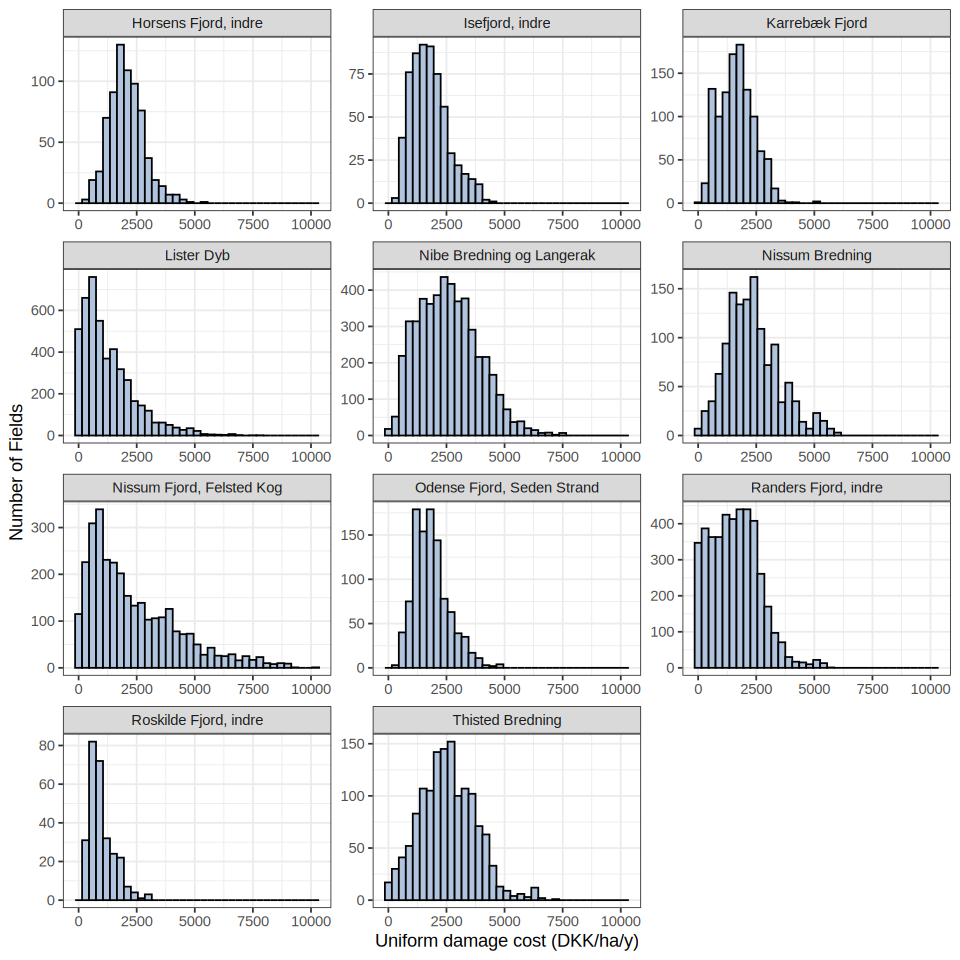
\includegraphics[width=1\textwidth]{figures/hist_uniform_dcost_hvede.png}
\caption{Distribution of Uniform Damage Cost (DKK/ha/y) - Winter wheat.}
\label{fig:hist_DC_uni_all}
\end{figure}


\subsection{Field-level Damage Costs}
\label{app:field-level-damage-costs}

\begin{table}[H]
\centering
\small
\caption{Area-weighted average uniform damage cost (DKK/ha/y) by crop type and catchment.}
\label{tab:uniform-full}
\resizebox{\textwidth}{!}{
\begin{threeparttable}
\begin{tabular}{lrrrrrrrrrrr}
\toprule
\textbf{Catchment} & \textbf{W. Wheat} & \textbf{S. Barley} & \textbf{Rapeseed} & \textbf{Maize} & \textbf{Rye/Trit.} & \textbf{Potatoes} & \textbf{Peas} & \textbf{Oats/Mix.} & \textbf{S. Beet} & \textbf{Seeds} & \textbf{Roughage} \\
\midrule
Lister Dyb                 & 1,263.4 & 1,292.8 & 1,102.2 & 1,320.9 & 1,284.8 & 1,245.3 & 1,060.1 & 1,060.4 &   983.0 & 2,129.6 & 1,328.2 \\
Nissum Bredning            & 2,237.3 & 2,376.7 & 2,213.5 & 3,117.8 & 2,267.6 & 1,948.4 &     ---  & 1,995.3 & 1,216.5 & 1,892.4 & 2,735.4 \\
Nissum Fjord, Felsted Kog  & 2,498.5 & 2,208.0 & 2,639.6 & 2,501.7 & 2,683.3 & 1,635.0 & 2,829.9 & 6,357.9 & 2,960.7 & 1,996.5 & 2,726.7 \\
Thisted Bredning           & 2,415.9 & 2,621.9 & 2,540.2 & 2,456.2 & 3,126.9 & 2,606.1 & 3,075.0 & 2,040.0 & 3,440.2 & 1,269.4 & 2,470.8 \\
Nibe Bredning og Langerak  & 2,806.9 & 2,591.0 & 2,456.3 & 2,496.5 & 2,513.9 & 2,153.8 & 2,479.3 & 3,008.0 & 1,197.2 & 2,621.4 & 2,566.2 \\
Randers Fjord, indre       & 1,742.5 & 1,661.4 & 1,649.0 & 1,216.6 & 1,560.7 & 1,239.2 & 1,478.1 & 1,624.3 & 1,673.8 & 1,392.5 & 1,360.9 \\
Horsens Fjord, indre       & 2,164.4 & 2,153.9 & 1,993.7 & 1,765.8 & 2,036.8 &     ---  & 1,676.5 & 1,962.5 &     ---  & 1,778.8 & 1,910.1 \\
Odense Fjord, Seden Strand & 1,899.4 & 1,746.7 & 1,772.2 & 1,929.5 & 1,814.8 &     ---  & 1,629.6 & 1,695.7 &     ---  & 2,045.0 & 2,266.1 \\
Isefjord, indre            & 1,637.5 & 2,015.9 & 1,746.8 & 2,155.6 & 1,416.5 & 2,149.7 & 1,930.5 & 1,614.0 &     ---  & 1,510.8 & 1,980.8 \\
Karrebæk Fjord             & 1,664.3 & 1,681.3 & 1,792.9 & 1,411.4 & 1,591.9 &     ---  & 1,379.0 & 1,692.2 & 1,766.0 & 1,563.9 & 1,697.3 \\
Roskilde Fjord, indre      &   979.6 & 1,031.7 & 1,027.4 &     ---  & 1,171.7 &     ---  & 1,321.6 & 1,136.9 &     ---  & 1,013.9 &   759.6 \\
\bottomrule
\end{tabular}
\begin{tablenotes}
\footnotesize
\item \textit{Notes:} All values are measured in DKK per hectare per year, weighted by
area. Uniform refers to the EU average damage cost of 130.76 DKK/kg N.
`---' indicates fewer than 20 fields and is therefore not reported.
W.~Wheat = Winter Wheat; S.~Barley = Spring Barley; Rye/Trit.\ = Rye/Triticale;
Oats/Mix.\ = Oats/Mixed Cereals; S.~Beet = Sugar Beet.
\end{tablenotes}
\end{threeparttable}
}
\end{table}

\subsection{Profitability from the Perspective of Society}

\subsubsection{Profitability from the perspective of society - Spring Barley Reference}
\label{Profitability from the perspective of society - Spring Barley Reference}

\begin{table}[H]
\centering
\small
\caption{Average profitability from society's perspective (DKK/ha/year) based on specific damage costs under the spring barley scenario.}
\label{tab:dbii-vaarbyg-specific}
\begin{threeparttable}
\begin{tabular}{lrrrrr}
\toprule
\textbf{Catchment} & \textbf{Fields} & \textbf{DBII} & \textbf{Fine} &
\textbf{Coarse} & \textbf{Loamy} \\
\midrule\addlinespace
Lister Dyb                 & 4,499 &     $-$  & $-$ (1,154)    & $-$ (763)      & $-$ (2,582)      \\
Nissum Bredning            & 1,241 &     $-$  & $-$ (313)      & $-$ (177)      & $-$ (751)        \\
Nissum Fjord, Felsted Kog  & 2,959 & $-$2,031 & $-$1,894 (749) & $-$2,541 (576) & $-$1,914 (1,634) \\
Thisted Bredning           & 1,289 &     $-$  & $-$ (349)      & $-$ (180)      & $-$ (760)        \\
Nibe Bredning og Langerak  & 4,579 &     $-$  & $-$ (1,526)    & $-$ (590)      & $-$ (2,463)      \\
Randers Fjord, indre       & 4,165 & $-$2,296 & $-$2,368 (1,045) & $-$2,863 (594) & $-$2,169 (2,526) \\
Horsens Fjord, indre       &   699 & $-$4,208 & $-$3,789 (177) & $-$4,351 (93)  & $-$4,344 (429)   \\
Odense Fjord, Seden Strand & 1,019 & $-$2,773 & $-$2,788 (228) & $-$2,979 (129) & $-$2,736 (662)   \\
Isefjord, indre            &   562 & $-$3,617 & $-$3,172 (133) & $-$ (53)       & $-$3,757 (376)   \\
Karrebæk Fjord             & 1,080 &     $-$  & $-$ (261)      & $-$ (138)      & $-$ (681)        \\
Roskilde Fjord, indre      &   278 & $-$4,472 & $-$ (58)       & $-$ (43)       & $-$4,472 (177)   \\
\addlinespace\bottomrule
\end{tabular}
\end{threeparttable}
\end{table}

\begin{table}[H]
\centering
\small
\caption{Average profitability from society's perspective (DKK/ha/year) based on uniform damage costs under the spring barley scenario.}
\label{tab:dbii-vaarbyg-uniform}
\begin{threeparttable}
\begin{tabular}{lrrrrr}
\toprule
\textbf{Catchment} & \textbf{Fields} & \textbf{DBII} & \textbf{Fine} &
\textbf{Coarse} & \textbf{Loamy} \\
\midrule\addlinespace
Lister Dyb                 & 4,499 & $-$3,254 & $-$3,160 (1,154) & $-$3,630 (763)  & $-$3,192 (2,582) \\
Nissum Bredning            & 1,241 & $-$4,097 & $-$3,834 (313)   & $-$4,477 (177)  & $-$4,140 (751)   \\
Nissum Fjord, Felsted Kog  & 2,959 & $-$3,042 & $-$2,908 (749)   & $-$3,466 (576)  & $-$2,952 (1,634) \\
Thisted Bredning           & 1,289 & $-$3,360 & $-$3,933 (349)   & $-$3,597 (180)  & $-$3,117 (760)   \\
Nibe Bredning og Langerak  & 4,579 & $-$3,191 & $-$2,753 (1,526) & $-$3,605 (590)  & $-$3,384 (2,463) \\
Randers Fjord, indre       & 4,165 & $-$2,917 & $-$2,983 (1,045) & $-$3,464 (594)  & $-$2,795 (2,526) \\
Horsens Fjord, indre       &   699 & $-$4,427 & $-$4,010 (177)   & $-$4,576 (93)   & $-$4,562 (429)   \\
Odense Fjord, Seden Strand & 1,019 & $-$3,367 & $-$3,382 (228)   & $-$3,582 (129)  & $-$3,328 (662)   \\
Isefjord, indre            &   562 & $-$4,003 & $-$3,567 (133)   & $-$ (53)        & $-$4,141 (376)   \\
Karrebæk Fjord             & 1,080 & $-$3,750 & $-$3,759 (261)   & $-$4,286 (138)  & $-$3,674 (681)   \\
Roskilde Fjord, indre      &   278 & $-$4,695 & $-$ (58)         & $-$ (43)        & $-$4,695 (177)   \\
\addlinespace\bottomrule
\end{tabular}
\end{threeparttable}
\end{table}


\begin{figure}[H]
\centering
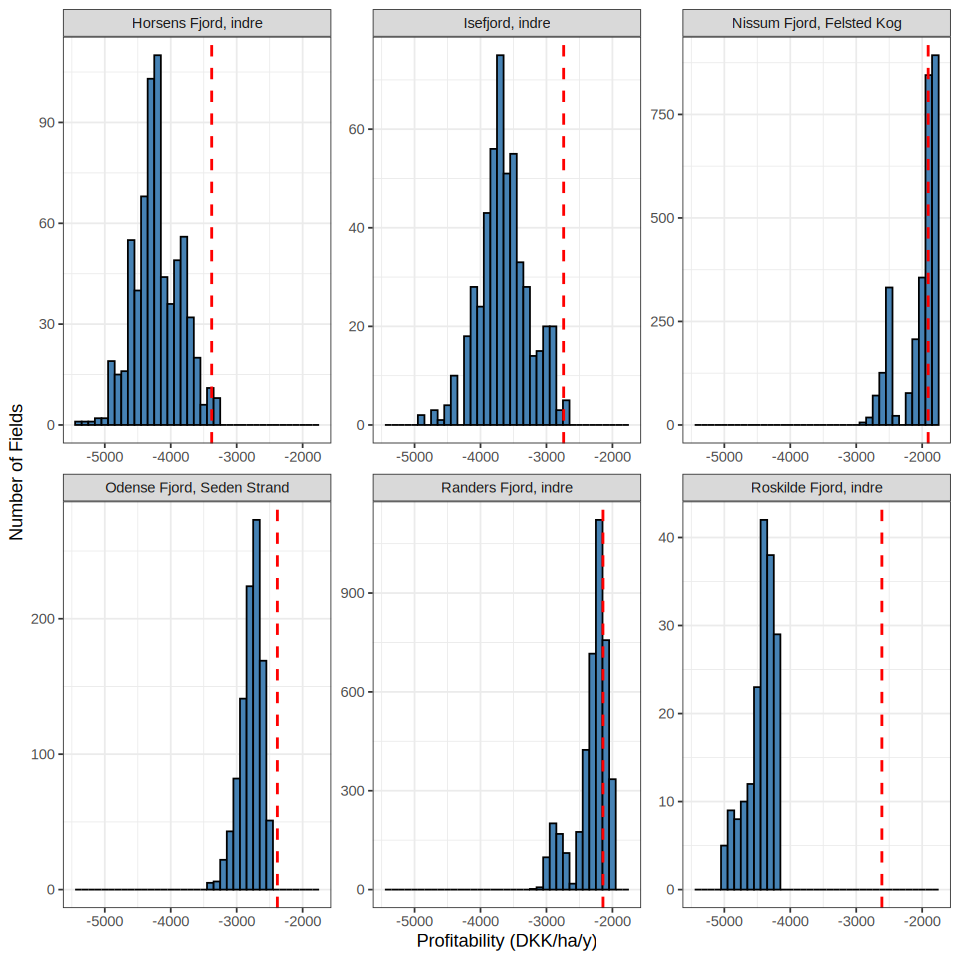
\includegraphics[width=0.9\textwidth]{figures/hist_specific_DBII_byg.png}
\caption{Distribution of (Specific) Profitability from Society's Perspective (DKK/ha/y). Red dashed line: catchment-level average private DBII (spring barley reference)}
\label{fig:social-dbii-specific-byg}
\end{figure} 

\begin{figure}[H]
\centering
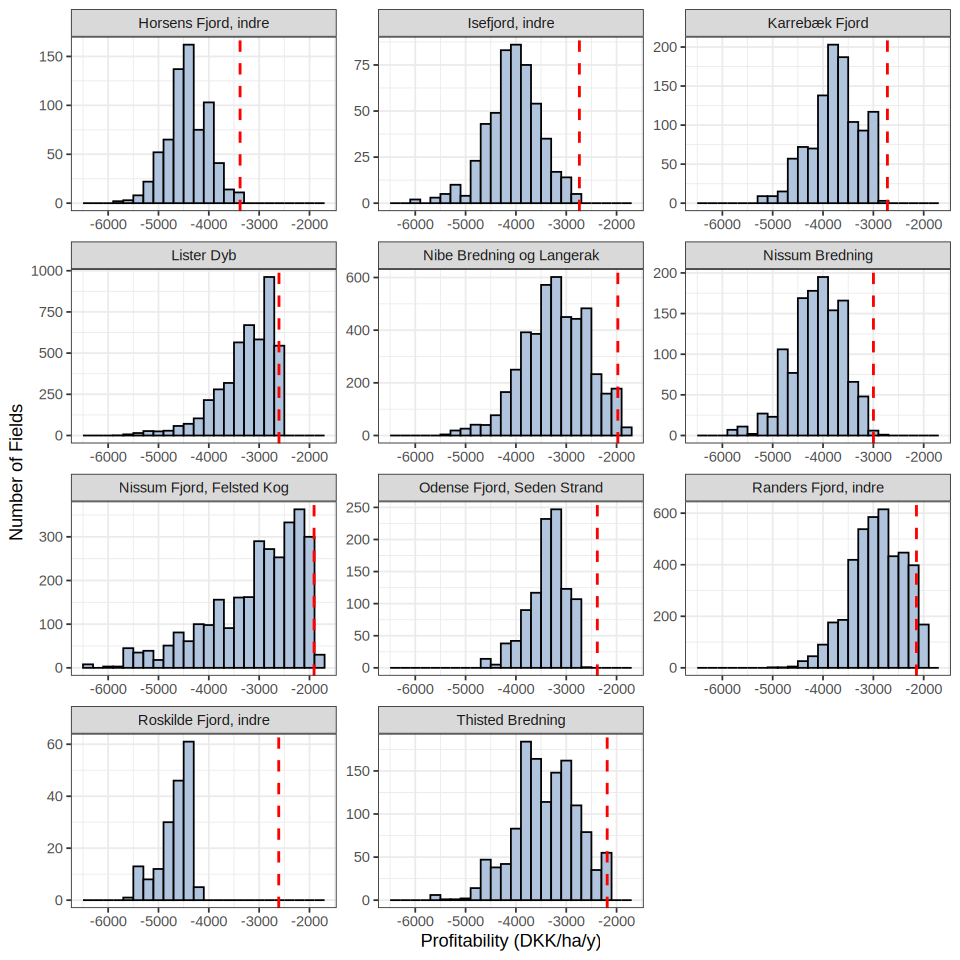
\includegraphics[width=0.9\textwidth]{figures/hist_uniform_DBII_byg.png}
\caption{Distribution of (Uniform) Profitability from Society's Perspective (DKK/ha/y). Red dashed line: catchment-level average private DBII (spring barley reference)}
\label{fig:social-dbii-uniform-byg}
\end{figure} 


\newpage


\section{Other}

\begin{figure}[H]
    \centering
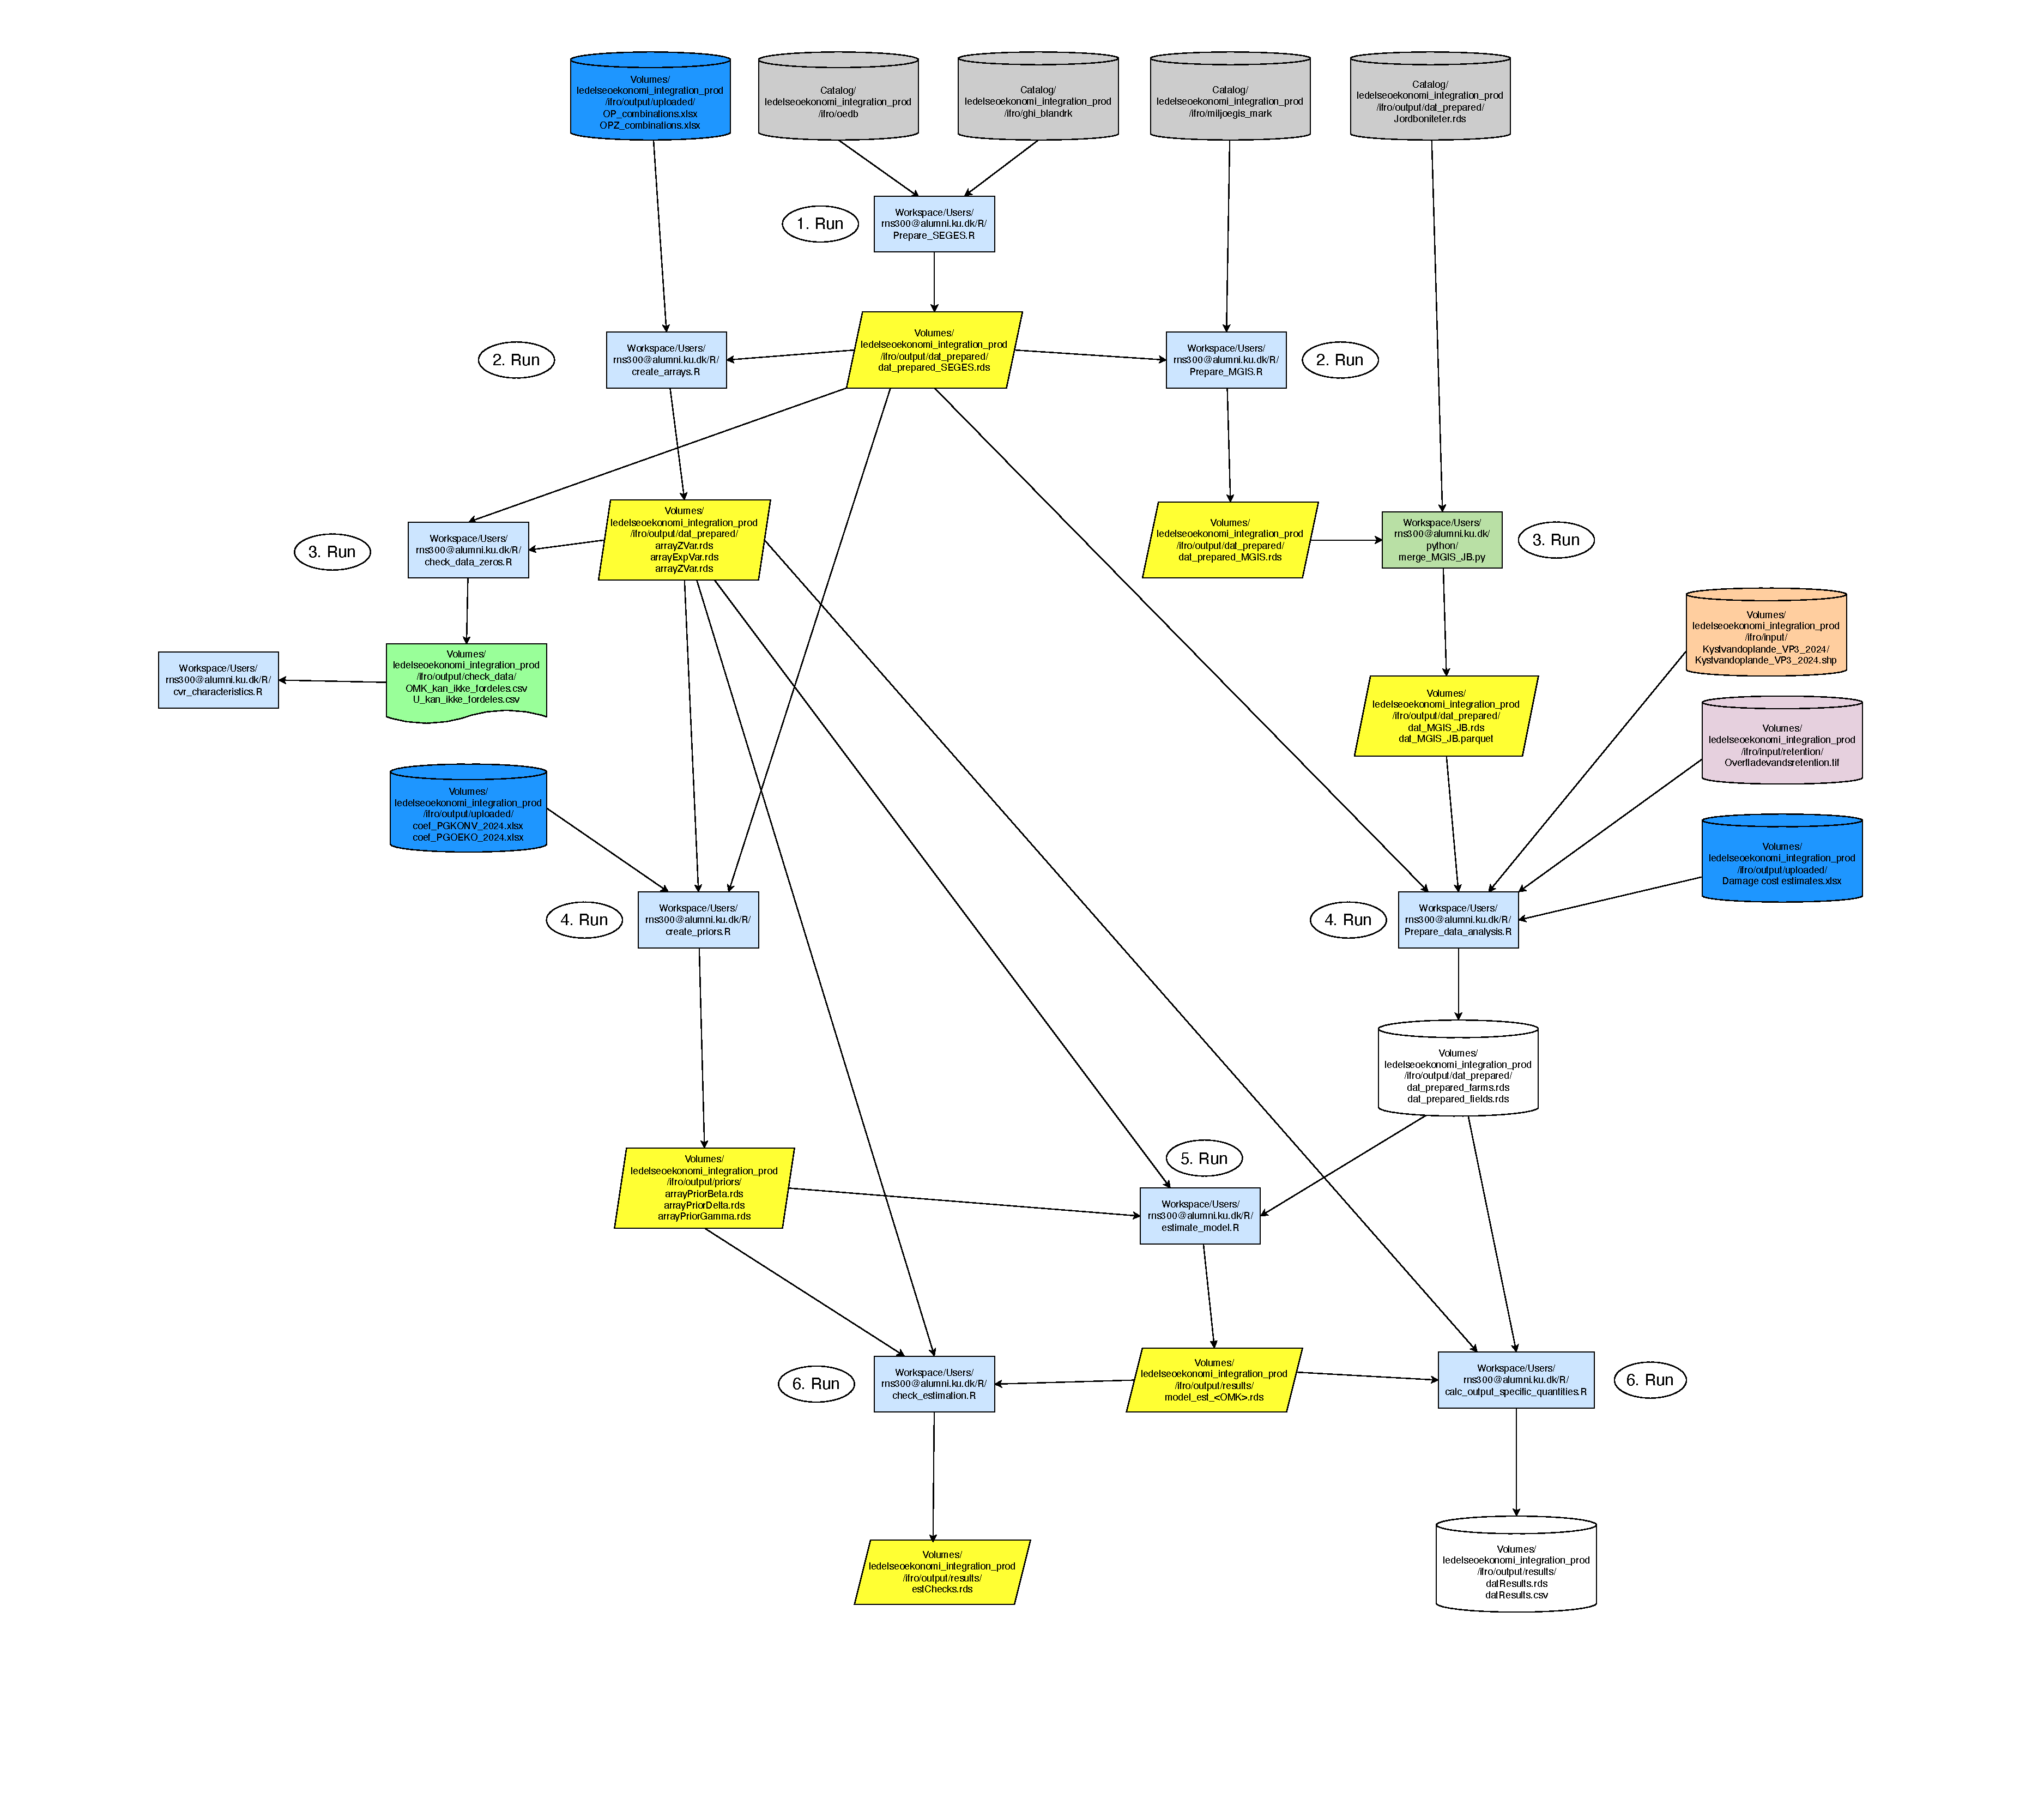
\includegraphics[width=1.1\textwidth]{figures/flowchart.pdf}
    \caption{Flowchart of notebooks and files used on Databricks. The figure is preliminary and should be updated with more connections.}
\end{figure}


\newpage


\bibliographystyle{apalike}
\bibliography{references}


\end{document}
